\documentclass[PhD]{iitmdiss}
%\documentclass[MS,twoside]{iitmdiss}
%\documentclass[MTech]{iitmdiss}
%\documentclass[BTech]{iitmdiss}
\usepackage{times}
 \usepackage{t1enc}
\usepackage{graphicx}
\usepackage{epstopdf}
\usepackage{hyperref} % hyperlinks for references.
\usepackage{amsmath} % easier math formulae, align, subequations \ldots
\usepackage{caption}
\usepackage[ruled,linesnumbered]{algorithm2e} % For algorithms
%\usepackage{subfig}
 \usepackage{subcaption}
 \usepackage{xfrac}
 \usepackage{nicefrac}
% \usepackage{footnote}
% \makesavenoteenv{tabular}
 \usepackage[font=small,labelfont=bf]{caption}
 \usepackage{booktabs}
 \usepackage{multirow}
 \usepackage[font={footnotesize}]{caption}
 \usepackage{amsthm}
\newtheorem{thm}{Theorem}[] % the main one
\newtheorem{lemma}[thm]{Lemma}
\theoremstyle{plain} % just in case the style had changed
 \newcommand{\thistheoremname}{}
 \newtheorem{genericthm}[thm]{\thistheoremname}
 \newenvironment{namedthm}[1]
   {\renewcommand{\thistheoremname}{#1}%
   \begin{genericthm}}
   {\end{genericthm}}
%%%%%%%%%%%%%%%%%%%%%%%%%%%%%%%
%\usepackage{ijcai17}
\SetKw{Continue}{continue}


\usepackage{macros}

\usepackage{latexsym} 



\newcommand{\clearemptydoublepage}{\newpage{\cleardoublepage}}


\begin{document}

%%%%%%%%%%%%%%%%%%%%%%%%%%%%%%%%%%%%%%%%%%%%%%%%%%%%%%%%%%%%%%%%%%%%%%
% Title page

\title{Gate sizing for energy efficient and secure digital designs.}

\author{Patanjali SLPSK}

\date{January 2018}
\department{COMPUTER SCIENCE AND ENGINEERING}

%\nocite{*}
\maketitle

%%%%%%%%%%%%%%%%%%%%%%%%%%%%%%%%%%%%%%%%%%%%%%%%%%%%%%%%%%%%%%%%%%%%%%
% Certificate

%\pagebreak
%\newpage
% \ 
%\thispagestyle{empty}
%\clearpage

\clearemptydoublepage
\certificate

\vspace*{0.5in}

\noindent This is to certify that the thesis titled {\bf Gate sizing for energy efficient and secure digital designs}, submitted by {\bf Patanjali SLPSK}, 
  to the Indian Institute of Technology, Madras, for
the award of the degree of {\bf Doctor of Philosophy}, is a bona fide
record of the research work done by him under our supervision.  The
contents of this thesis, in full or in parts, have not been submitted
to any other Institute or University for the award of any degree or
diploma.

\vspace*{1.5in}

\begin{singlespacing}
\hspace*{-0.25in}
\parbox{2.5in}{
\noindent {\bf Dr. Kamakoti Veezhinathan} \\
\noindent Research Guide \\ 
\noindent Professor \\
\noindent Dept. of Computer Science\\
\noindent IIT-Madras, 600 036 \\
} 

\end{singlespacing}
\vspace*{0.25in}
\noindent Place: Chennai\\
Date: January, 2018


%%%%%%%%%%%%%%%%%%%%%%%%%%%%%%%%%%%%%%%%%%%%%%%%%%%%%%%%%%%%%%%%%%%%%%
% Acknowledgements
\clearemptydoublepage
\acknowledgements
%To be written.
To be filled

% I am grateful to my primary thesis advisor Dr. Balaraman Ravindran from Computer Science and Engineering Department at IIT Madras. Without his constant guidance, motivation and perseverance with me, none of these works would have been completed. His courses of Introduction to Machine Learning and Introduction to Reinforcement Learning were my first step into the research world. Not only these courses carried a wealth of information on the current state of literature in the respective fields but they used to be hugely competitive which used to constantly motivate me to strive for excellence. Apart from our formal meetings every week, I used to catch him in his office or in the corridors or anywhere in the department whenever I had any doubts and we used to converse on them. One of his greatest influences on me is to inculcate the constant urge to collaborate with as many interested people as possible, both inside and outside of my immediate field of research. This became a huge contributing factor in the research that I conducted for this thesis.

% I am also grateful to my co-advisor Dr. Nandan Sudarsanam from Department of Management Studies at IIT Madras. It is from him that I first learned the most important factor of publication, how to properly write research papers in a concise and crisp manner. I fondly remember that how intensely he used to scrutinize my drafts for errors and incoherent ideas. His dedication and trust in my work are evident from this one incident during the ICML 2017 submission, when at 2 am in the night he called me up to correct portions of my draft. Also, his courses in Department of Management Studies are very enjoyable to attend and are very informative. Nobody can make you understand a complex idea in a simple way and yet retain all its subtleties as Nandan sir can and his courses used to reflect this idea.

% Another person who had a profound influence on me is Dr. K.P. Naveen from Electrical Engineering Department at IIT Tirupati who advised me on a significant portion of this thesis. I first attended one of his courses on Introduction to Probability Theory here at IIT Madras (when he was INSPIRE Faculty member here) and instantly liked the way he taught the complex idea of Probability theory in simple terms. Even though the area of Multi-armed bandits is not his core research area, yet we collaborated on this topic which led to multiple publications. I fondly remember his rigor and patience with me while correcting the theoretical portions of my draft, the most important section of any bandit research paper.

% I am also grateful to Dr. L.A. Prashanth from Computer Science and Engineering Department at IIT Madras in my initial days of research for advising me on a significant portion of stochastic multi-armed bandits. He is up-to-date with all the research work in this area and my interactions with him always led to new ideas and a broader way to look at a problem. All collaborations do not always lead to publications and I hope that our future interactions will lead to a more fruitful outcome.

% While writing this thesis I must also acknowledge the contributions of Dr. Odalric-Ambrym Maillard from INRIA, SequeL Lab at Lille, France where I went for winter internship from September to December 2017. He is one of the most inspiring researchers that I met in my foray into the research world. He was always available at his office, always working on interesting ideas and always interested to listen to any idea that I came up with. The best thing about him that I can fondly relate to is that he never rejected any idea even though they were initially outrageous, but used to guide me slowly towards the reason on why they would fail in the long run. Similarly, I must also thank Dr. Branislav Kveton from Adobe Research, San Jose, whom I met on the sidelines of IJCAI 2017 who gave me a lot of feedback on how to improve my work on Thresholding Bandits. 

% I am thankful to the other members of my committee for their constant support and guidance. I am especially thankful to Dr.  Sutanu Chakraborti for his trust on me. I fondly remember that whenever we used to meet we used to converse in Bengali and he used to constantly motivate me to work more. His course on Natural Language Processing is a very enjoyable course and the project on humor generation that I did under his supervision is one of most interesting projects I did in my IIT Madras coursework. I am also thankful to my Dr. Nirav P Bhatt and my committee chair Dr. P Sreenivasa Kumar for being always available for me.


% I am thankful towards a host of my colleagues in the RISE Lab at Computer Science and Engineering Department where I spent a significant time while conducting research at IIT Madras. Thanks Patanjali for creating such an environment in the lab, conducive to research. I also thank my first roommate Priyesh for making my first semester so livable on the campus. In the course of time, I made more friends who contributed in making my life at IIT Madras memorable; Shashank, Siddharth, Deepak, Varun, Tarun, Madhuri, Ditty, Ahana, without you people life at IIT Madras would have been boring. There are several members of IPCV lab to whom I am grateful for making my stay at IIT Madras very memorable especially I must thank Nimisha, Abhijith, and Karthik for being such wonderful friends. I am also grateful towards my father, mother, brother, and sister-in-law Sarah for providing me constant motivation in my research and personal life. 

% Last but not the least, I must thank Dr. A.P. Vijay Rengarajan from Electrical Engineering Department at IIT Madras. He was also conducting research for his doctoral studies in the IPCV lab and it his from him that I learned the true meaning of dedication towards research. This dedication of him, of course, showed up in all the publications he got but most of all he was always there, listening to all my concerns on a host of issues that I faced in my research and personal life. Vijay without you life at IIT Madras would not have been same.

% Finally, I must acknowledge the influence of Dr. Sven Koenig whom I met on the sidelines of IJCAI 2017 in the "Lunch with  A Fellow" event. That four-hour interaction with him is a memory I cherish because we talked about every possible aspect of a researcher's life and how to conduct good research. In the end, he said to me the three mantras of conducting good research; shed ego, collaborate and learn something new every day.

% %Every day from 9 am to 6 pm for 365 days a year he was available in the lab, sitting in front of his desktop and working tirelessly.


%%%%%%%%%%%%%%%%%%%%%%%%%%%%%%%%%%%%%%%%%%%%%%%%%%%%%%%%%%%%%%%%%%%%%%
% Abstract
\clearemptydoublepage
\abstract

%\noindent KEYWORDS: \hspace*{0.5em} \parbox[t]{4.4in}{Reinforcement Learning, Bandits, UCB, EUCBV, Thresholding Bandits,  AugUCB, changepoint detection, SECPD.}

%\noindent KEYWORDS: \hspace*{0.5em} \parbox[t]{4.4in}{Reinforcement Learning, Stochastic Bandits, UCB, UCBV, EUCBV, Thresholding Bandits, APT, AugUCB}

\vspace*{24pt}
\noindent Computers have evolved from being glorified calculators that occupied the space of a large building to small pervasive devices. This rapid growth, however, has increased the expectations that the end user places on today's digital devices which, in turn, has increased the number of constraints on the device. This thesis considers two such objectives viz, power and security and proposes design level techniques to address the same.

Today's devices are expected to be extremely performance efficient with both servers and mobile phones expected to run the same workload, e.g., statistical inference algorithms, smaller in size and have a lower energy footprint to enable ubiquity in deployment. This creates challenges for digital designers as these constraints are orthogonal causing designers to sacrifice one or more of these objectives. The exponential growth in the number of EDGE devices has also impacted the device manufacturing time which creates a unique challenge for the digital designer as the design is now expected to meet three orthogonal constraints in a short amount of time. Our proposed MLTimer solution presented in this thesis addresses this problem that uses a novel data-driven algorithm which lets the designer re-use solutions from previously optimized circuits to meet the power constraints for  a given design. We show that the proposed solution outperforms the state-of-the-art solutions by evaluating it on the ISPD2012, ISPD2013 benchmark circuits. We compare the results with a commercial EDA flow by evaluating the proposed solution to optimize a state-of-the-art embedded processor running Linux.

The recent Meltdown and Cambridge Analytica data leaks have sensitized the common man to the importance of a secure software and hardware computing platform. While software vulnerabilities can be fixed by implementing a patch with minimal overheads, hardware vulnerabilities, otherwise known as side-channels, are harder to detect and correct. In this thesis, we consider the problem of power side-channels on embedded devices and propose a gate-sizing based solution to reduce the risk of a digital device through the power side-channel. Our proposed solution, Karna, is the first design level solution. We quantify the effectiveness of Karna along with the area, delay and performance overheads by evaluating the proposed scheme on three different block ciphers.


%This thesis studies the following topics in the area of Reinforcement Learning: classic Multi-armed bandits in stationary distribution with the goal of cumulative regret minimization using variance estimates and Thresholding bandits in pure exploration fixed-budget setting with the goal of instantaneous regret minimization also using variance estimates. The common underlying theme is the study of bandit theory and its application in various types of environments. In the first part of the thesis, we study the classic multi-armed bandit problem with a stationary distribution, one of the first settings studied by the bandit community and which successively gave rise to several new directions in bandit theory. We propose a novel algorithm in this setting and compare both theoretically and empirically its performance against the available algorithms. Our proposed algorithm termed as Efficient-UCB-Variance (EUCBV) is the first arm-elimination algorithm which uses variance estimation to eliminate arms as well as achieve an order optimal regret bound. Empirically, we show that EUCBV outperforms most of the state-of-the-art algorithms in the considered environments. In the next part, we study a specific type of stochastic multi-armed bandit setup called the thresholding bandit problem and discuss its usage, available state-of-the-art algorithms on this setting and our solution to this problem. We propose the Augmented-UCB (AugUCB) algorithm which again uses variance and mean estimation along with arm elimination technique to conduct exploration. We give theoretical guarantees on the expected loss of our algorithm and also analyze its performance against state-of-the-art algorithms in numerical simulations in multiple synthetic environments. 

%The thesis studies the following topics in the area of Reinforcement Learning: Multi-armed Bandits, Multi-armed bandits in stationary distribution with the goal of cumulative regret minimization and Thresholding bandits in pure exploration setting. The common underlying theme is the study of bandit theory and its application in various types of environments. We start with a general introduction to Multi-armed bandits, its connection to the wider reinforcement learning theory and then we discuss the various types of bandits available in the literature. Then we delve deep into the classic multi-armed bandit problem in stationary distribution, one of the first setting studied by the bandit community and which successively gave rise to several new directions in bandit theory. We propose a novel algorithm in this setting and compare both theoretically and empirically its performance against the available algorithms in this setting. Subsequently, we study a very specific type of bandit setup called the thresholding bandit problem and discuss extensively on its usage, available state-of-the-art algorithms on this setting and our solution to this problem. We give theoretical guarantees on the expected loss of our algorithm and also analyze its performance against state-of-the-art algorithms in numerical simulations in multiple synthetic environments. 

%, and analysis of bandit theory in piece-wise stationary distributions

%Finally, we study the notion of piece-wise stationary distribution and how available bandit algorithms can be modified to perform well in this setting. We propose a set of algorithms for this setting with the goal of minimizing cumulative regret which uses various techniques ranging from changepoint detection mechanism to aggregation of experts.

%\pagebreak

%%%%%%%%%%%%%%%%%%%%%%%%%%%%%%%%%%%%%%%%%%%%%%%%%%%%%%%%%%%%%%%%%
% Table of contents etc.
\clearemptydoublepage
\begin{singlespace}
\tableofcontents
%\thispagestyle{empty}

\clearemptydoublepage
\listoftables
\addcontentsline{toc}{chapter}{LIST OF TABLES}


\clearemptydoublepage
\listoffigures
\addcontentsline{toc}{chapter}{LIST OF FIGURES}
\end{singlespace}


%%%%%%%%%%%%%%%%%%%%%%%%%%%%%%%%%%%%%%%%%%%%%%%%%%%%%%%%%%%%%%%%%%%%%%
% Abbreviations
\clearemptydoublepage
\abbreviations

\noindent 
\begin{tabbing}
xxxxxxxxxxx \= xxxxxxxxxxxxxxxxxxxxxxxxxxxxxxxxxxxxxxxxxxxxxxxx \kill
%\textbf{RL}   \> Reinforcement Learning \\
%\textbf{MAB} \> Multi-armed Bandit \\
%\textbf{SMAB} \> Stochastic Multi-armed Bandit \\
%\textbf{UCB} \> Upper Confidence Bound \\
%\textbf{MOSS} \> Minimax Optimal Strategy in the Stochastic case \\
%\textbf{UCBV} \> Upper Confidence Bound Variance \\
%\textbf{OCUCB} \> Optimally Confident Upper Confidence Bound \\
%\textbf{KLUCB} \> Kullback–Leibler Upper Confidence Bound \\
%\textbf{TS} \> Thompson Sampling \\
%\textbf{EUCBV} \> Efficient Upper Confidence Bound Variance \\
%\textbf{TBP} \> Thresholding Bandit Problem \\
%\textbf{UCBE} \> Upper Confidence Bound Exploration\\
%\textbf{UCBEV} \> Upper Confidence Bound Exploration Variance\\
%\textbf{UA} \> Uniform Allocation \\
%\textbf{SR} \> Successive Reject \\
%\textbf{CSAR} \> Combinatorial Successive Accept Reject \\
%\textbf{APT} \> Anytime Parameter-free Thresholding \\
%\textbf{AugUCB} \> Augmented Upper Confidence Bound \\
\textbf{APT} \> Anytime Parameter-free Thresholding \\
\textbf{AugUCB} \> Augmented Upper Confidence Bound \\
%BIB
\textbf{BU} \> Bayes-UCB \\
\textbf{CCB} \> Combined Confidence Bound \\
%CPD
%CPDI
\textbf{CSAR} \> Combinatorial Successive Accept Reject \\
%CUSUM
%DBLP
\textbf{DMED} \> Deterministic Minimum Empirical Divergence \\
\textbf{DTS} \> Discounted Thompson Sampling \\
\textbf{DUCB} \> Discounted UCB \\
%DVI
\textbf{EUCBV} \> Efficient Upper Confidence Bound Variance \\
%EVE
\textbf{EXP3} \> Exponential Exploration Exploitation \\
\textbf{EXP3IX} \> EXP3 Implicit Exploration \\
\textbf{GCTS} \> Global Change-ponit Thompson Sampling \\
%GK
%IITM
\textbf{KL} \> Kullback–Leibler \\
\textbf{KLUCB} \> Kullback–Leibler Upper Confidence Bound \\
%KT
%LHS
\textbf{LUCB} \> Lower Upper Confidence Bound \\
\textbf{MAB} \> Multi-armed Bandit \\
\textbf{MDP} \> Markov Decision Process \\
\textbf{MOSS} \> Minimax Optimal Strategy in the Stochastic case \\
%MS
\textbf{OCUCB} \> Optimally Confident Upper Confidence Bound \\
%\textbf{OTS} \> Oracle Thompson Sampling \\
%PDF
\textbf{RL}   \> Reinforcement Learning \\
\textbf{RExp3}   \> Restarting EXP3 \\
\textbf{SAR} \> Successive Accept Reject \\
%SECPD
\textbf{SMAB} \> Stochastic Multi-armed Bandit \\
\textbf{SR} \> Successive Reject \\
\textbf{SW-UCB} \> Switching Window UCB \\ 
\textbf{TBP} \> Thresholding Bandit Problem \\
\textbf{TS} \> Thompson Sampling \\
\textbf{UA} \> Uniform Allocation \\
\textbf{UCB} \> Upper Confidence Bound \\
\textbf{UCBE} \> Upper Confidence Bound Exploration\\
\textbf{UCBEV} \> Upper Confidence Bound Exploration Variance\\
\textbf{UCBV} \> Upper Confidence Bound Variance \\
%URL



\end{tabbing}

%\pagebreak

%%%%%%%%%%%%%%%%%%%%%%%%%%%%%%%%%%%%%%%%%%%%%%%%%%%%%%%%%%%%%%%%%%%%%%
% Notation

\clearemptydoublepage
\chapter*{\centerline{NOTATION}}
\addcontentsline{toc}{chapter}{NOTATION}

\begin{singlespace}
\begin{tabbing}
xxxxxxxxxxx \= xxxxxxxxxxxxxxxxxxxxxxxxxxxxxxxxxxxxxxxxxxxxxxxx \kill
\textbf{$T$} \> Time horizon\\
\textbf{$\A$} \> Set of arms\\
\textbf{$K$} \> Total number of arms\\
\textbf{$\pi$}   \> Policy of an agent \\
\textbf{$D_i$}  \> Reward distribution of $i$-th arm \\
\textbf{$r_i$}  \> Expected mean of $D_i$ for the $i$-th arm \\
\textbf{$\hat{r}_i$}  \> Sample mean of the $i$-th arm \\
\textbf{$X_{i,t}$} \> Reward obtained for the $i$-th arm at the $t$-th timestep\\
\textbf{$z_i$}  \> Number of times arm $i$ is pulled\\
\textbf{$\sigma_i$} \> Standard Deviation of the $i$-th arm\\
\textbf{$v_i$} \> Variance of the $i$-th arm\\
\textbf{$\Delta_i$} \> Gap of the $i$-th arm\\
\textbf{$\Delta$} \> Minimal gap amongst all arms\\
\textbf{$\tau$} \> Threshold\\
\textbf{$H_1$} \> Hardness with Mean-$1$\\
\textbf{$H_2$} \> Hardness with Mean-$2$\\
\textbf{$H_{\sigma,1}$} \> Hardness with Mean and Standard Deviation-$1$\\
\textbf{$H_{\sigma,2}$} \> Hardness with Mean and Standard Deviation-$2$\\
\textbf{$\rho$} \> Parameter for tuning length of of confidence interval\\
\textbf{$\psi$} \> Exploration parameter\\
\textbf{$m$} \> Round number\\
\textbf{$R_T$} \> Cumulative regret till horizon $T$\\
\textbf{$SR_t$} \> Simple regret at $t$-th timestep\\
\end{tabbing}
\end{singlespace}

%\pagebreak
%\clearpage

% The main text will follow from this point so set the page numbering
% to arabic from here on.



%%%%%%%%%%%%%%%%%%%%%%%%%%%%%%%%%%%%%%%%%%%%%%%%%%
% Introduction.
\clearemptydoublepage
\pagenumbering{arabic}
\chapter{Introduction}
\label{chap:intro}

\section{Reinforcement Learning}
\label{intro}
One of the significant moments that has shaped human history was the invention of the computer. What essentially started out as an attempt to replace and replicate simple arithmetic functions now surrounds us on a day-to-day basis taking care of our transport, health, finance and ingratiating itself into our daily lives more and more. 

This evolution has largely been made possible due to the invention of the transistor by Bell & Schokley in 1951 which caused computers to go from the size of an airplane hangar to tiny microscopic devices.  The invention of the transistors enabled chip designers to meet the ever increasing user requirements by halving the size of the transistors and thereby doubling the number of transistors that could be packed into the same area. This phenomenon also dubbed as Moore’s law has enabled chip designers meet the exponentially increasing functionality requirements.

In addition to increasing functionality, digital devices are also expected to meet additional constraints which can be enumerated using the tuple {Power, Area and Delay}. Depending on the platform in which it gets deployed, the chip designer might have to optimize the same design to meet  two orthogonal constraints. For example, when building a server, the processor is expected to be fast while the power and area requirements are relaxed but on the other hand if the same processor is to be used on a IoT device, the designer might have to optimise the design for low power, smaller area while the device might not be expected to perform at the same speed as the server. **{ Can we rewrite it with a better example?}

We now discuss the three key objectives that a given digital design is expected to meet. 
\begin{enumerate}
    \item \textbf{Delay} With each passing generation 
\end{enumerate}





%Computers have evolved from being simple calculators to devices that can perform complex operations that are employed in various aspects of our day-to-day lives.  
%This evolution has been 

%For the last 70 years, chip designers have been able to meet this expectation by leveraging Moore's law and adding more transistors.  

%Today digital devices can be broadly classified into three different classes \begin{enumerate}
 %   \item Embedded devices: These devices are expected to interact with various aspects of a user's environment such as temperature, motion etc. and make decisions on the fly. The emergence of Internet of Things as a popular networking paradigm in the last 3 years has led to an increase in the demand for such devices. These class of devices typically application specific and perform either "send and send" or lightweight computation at the
%\end{enumerate}

%In this evolution, the expectations of the end-user from each generation has been increasing. While initial generations were expected to merely speed-up arithmetic operations, the development of commercial compute devices starting with Intel's 4004 processor has led to these devices perform complex mathematical functions at a faster rate, on a smaller device by using a little energy as possible. 












% In today's world, artificial intelligence has proved to be a game-changer in designing agents that interact with an evolving environment and make decisions on the fly. The main goal of artificial intelligence is to design artificial agents that make dynamic decisions in an evolving environment. In pursuit of these, the agent can be thought of as making a series of sequential decisions by interacting with the dynamic environment which provides it with some sort of feedback after every decision which the agent incorporates into its decision-making strategy to formulate the next decision to be made. A large number of problems in science and engineering, robotics and game playing, resource management, financial portfolio management, medical treatment design, ad placement, website optimization and packet routing can be modeled as sequential decision-making under uncertainty. Many of these real-world interesting
% sequential decision-making problems can be formulated as reinforcement learning (RL) problems (\citep{bertsekas1996neuro}, \citep{sutton1998reinforcement}). In an RL problem, an agent interacts with a dynamic, stochastic, and unknown environment, with the goal of finding an action-selection strategy or policy that optimizes some long-term performance measure. Every time when the agent interacts with the environment it receives a signal/reward from the environment based on which it modifies its policy. The agent learns to optimize the choice of actions over several time steps which is learned from the sequences of data that it receives from the environment. This is the crux of online sequential learning. 

%     This is in contrast to supervised learning methods that deal with labeled data which are independently and identically distributed (i.i.d.) samples from the considered domain and train some classifier on the entire training dataset to learn the pattern of this distribution to predict the labels of future samples (test dataset) with the assumption that it is sampled from the same domain. In contrast to this, an RL agent learns from the samples that are collected from the trajectories generated by its sequential interaction with the system. For an RL agent, the trajectory consists of a series of sequential interactions whereby it transitions from one state to another following some dynamics intrinsic to the environment while collecting the reward till some stopping condition is reached. This is known as an episode. Here, for an action $i_t$ taken by the agent at the $t$-th timestep, the agent transitions from its current state denoted by $S_{i,t}$ to state $S_{i,t+1}$ and observes the reward $X_{i,t}$. An illustrative image depicting the reinforcement learning scenario is shown in Figure \ref{fig:rl}.

% \begin{figure}[!th]
% \includegraphics[scale=0.45]{Chapter1/img/RL1.png}
% \caption{Reinforcement Learning}
% \label{fig:rl}
% \end{figure}


    
    
% %To express an RL problem more formally, we have to define the idea of Markov Decision Process (MDP) which consists of states, actions, transition probabilities, and rewards which in turn helps in deciding the strategy to be followed by the agent. 

% %An MDP consists of states


\section{Connection between Reinforcement Learning and Bandits}
\label{conn:Bandits}
%\input{Chapter1/connBandits}

\section{Why study Bandits?}
\label{study}
%\input{Chapter1/studyBandit}

\section{Motivation}
\label{motivation}
%\section{Motivation for Integrating Security requirements into an EDA Flow}
\label{sec:motivation}

%In this section, we provide a concrete example that highlights the fact that existing EDA optimizations indeed have an effect on the security of the device. 
%need for a security-aware EDA flow that optimizes security along with the typical requirements. We take an AES-128 design and synthesize it to generate six different netlists each of which is optimized to meet a different objective such as low power, high performance \& smaller area, low power \& smaller area, and high performance \& low power. % as shown in Table~\ref{tab:design}. 
%The design configurations with their area, delay, and power numbers are shown in Table~\ref{tab:design}. We then analyze the side-channel resistance of each netlist using the Mean Traces to Leak (MTL) metric defined in Section~\ref{}. %The number of power traces needed to guess the key, called mean time for disclosure (MTD), is shown in the fourth column of Table~\ref{tab:design}. A higher MTD value indicates that the attacker needs to collect large number of samples in order to guess the AES key and a smaller MTD value indicates that the device can be easily exploited via the power side-channel.

% \todo[inline]{table 1 hardly makes sense! out of 6 designs on the 3rd one actually serves the purpose.}
\begin{table}[t!]
\scriptsize
\centering

\caption{Impact of design requirements on Area, Power, Delay and the magnitude of TVLA score at the end of 4000 traces for an AES design.  }
\begin{tabular}{|c|c|c|c|c|c|}

\hline

\textbf{\begin{tabular}[c]{@{}c@{}}Design \\ Choices\end{tabular}} & \textbf{Area} & \textbf{\begin{tabular}[c]{@{}c@{}}Delay \\ (ns)\end{tabular}} & \textbf{\begin{tabular}[c]{@{}c@{}}Static\\  Power ($\mu W$)\end{tabular}} & \textbf{TVLA}\\ \hline
I -- Area $\downarrow$ Power $\downarrow$ &       78883        &                  0.48                                              &                            492.4                                  & 11.077                                                                          \\ \hline
II  -- Area $\downarrow$        &        58439       &                 0.48                                               &    602.42             &  11.41                                                                                                            \\ \hline
III -- Area $\downarrow$ Delay $\downarrow$      &       82545        &               0.47                                                 &    513.40               & 8.22  \\ \hline
IV -- Power $\downarrow$ Delay $\downarrow$     &     102256          &             0.47                                                   &               683.41     & 10.65 \\ \hline
V --    Power $\downarrow$ &    79097           &             0.48                                                   &     482.80              &   9.95\\ \hline
VI -- Delay $\downarrow$    &        91822       &        0.32                                                        &     2105.8                  &  13.97       

\\ \hline

\end{tabular}
\label{tab:design}
\end{table}
\begin{figure}[t!]
\centering
  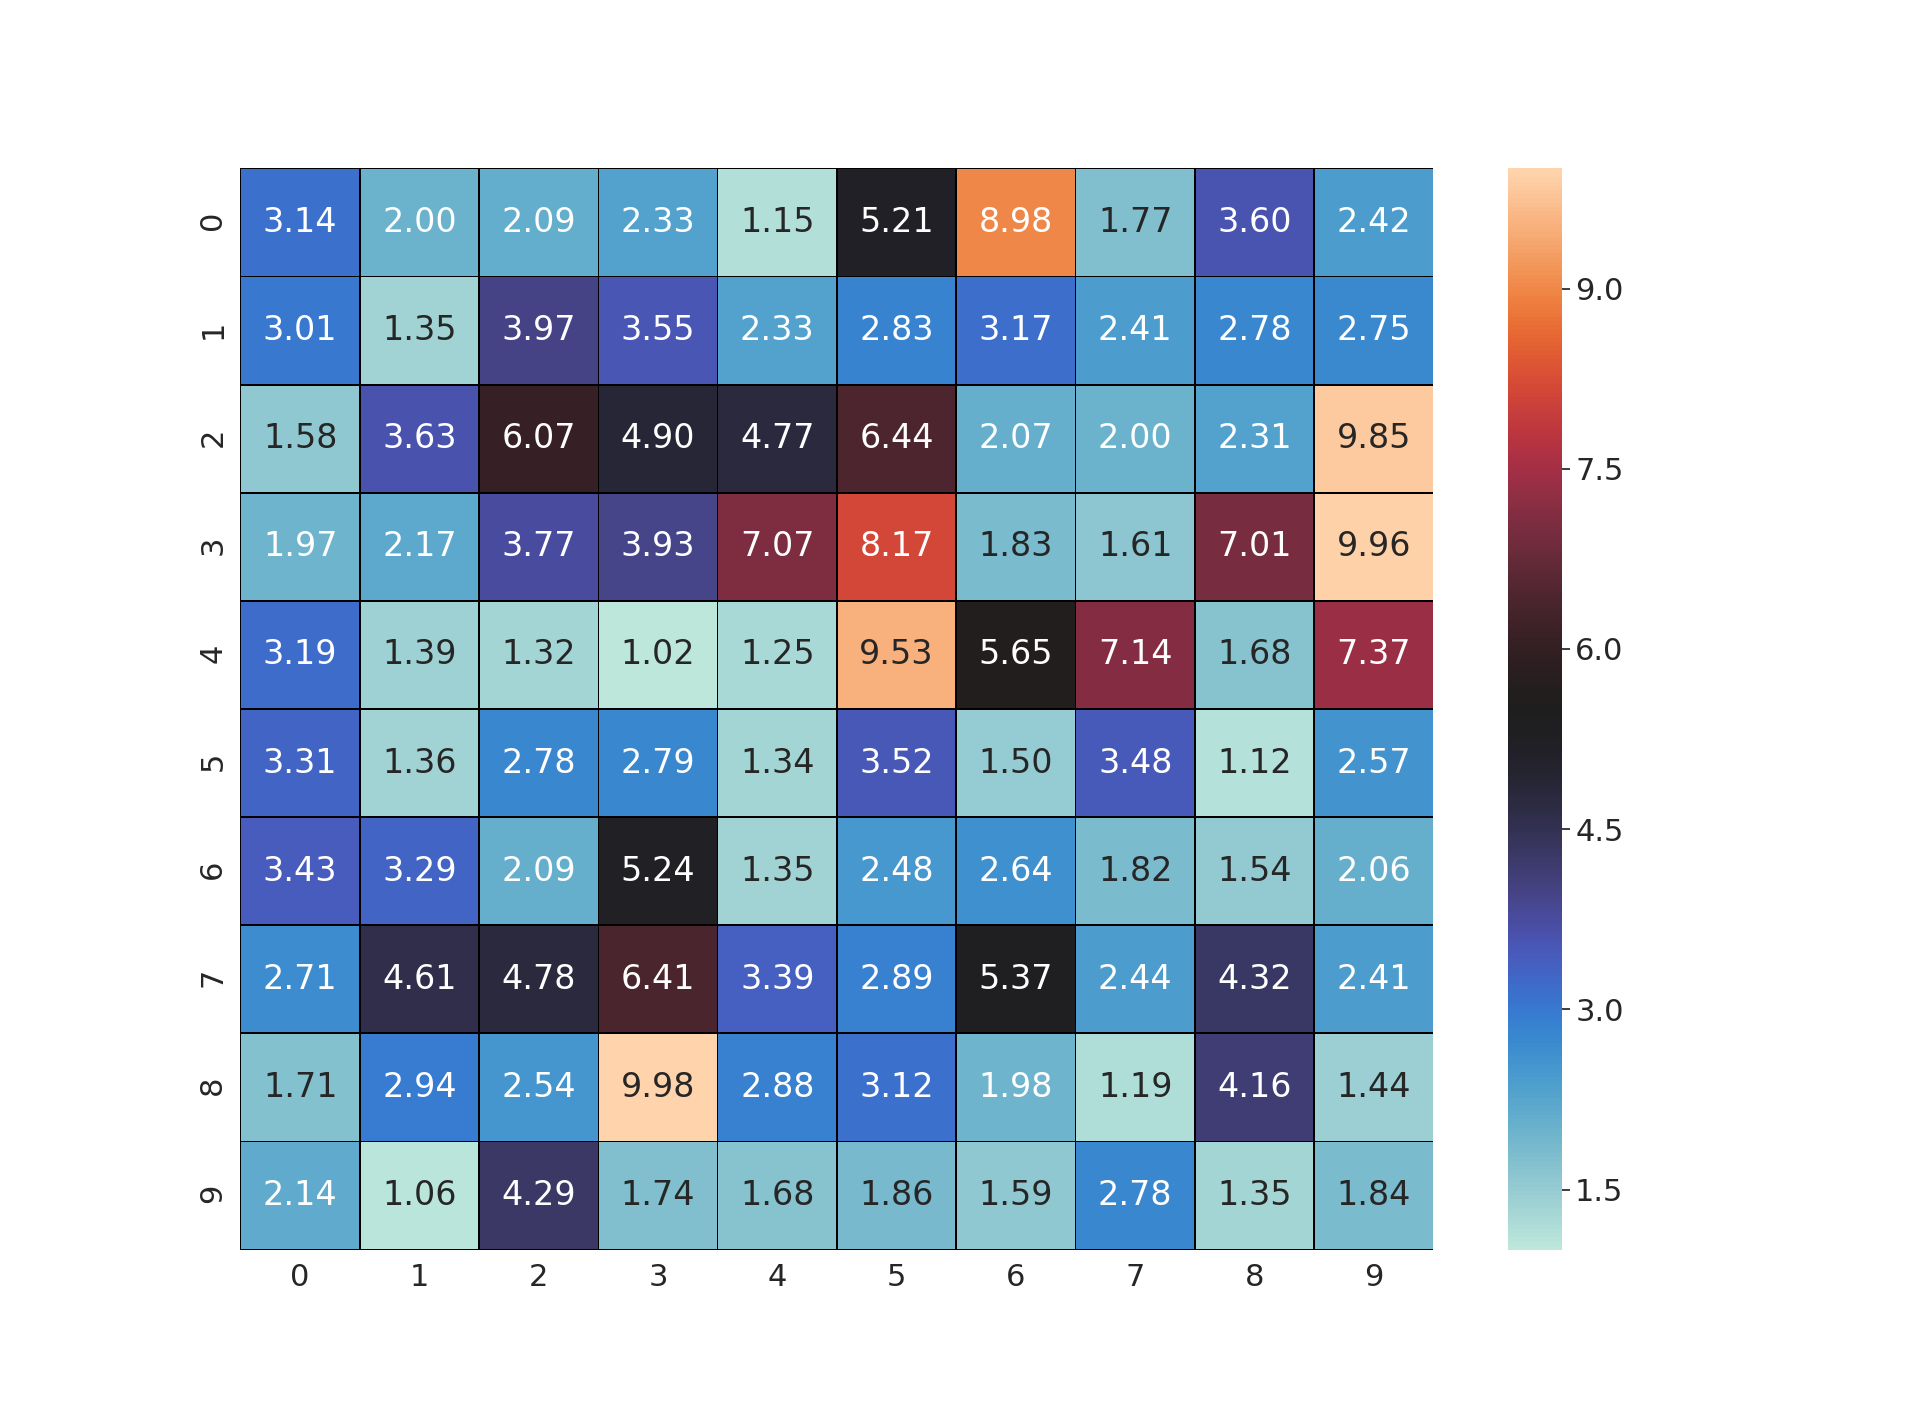
\includegraphics[scale=0.20]{Chapter4/fig/aes_before.png}  
\caption{The TVLA profile of the AES design, with the design divided into a $10\times 10$ grid and the TVLA score of each cell calculated independently. Of the 100 cells, 21 have a TVLA score greater than 4.5. The overall TVLA score of the netlist is 8.22. }
\label{fig:aesopt}
\end{figure}

In this section, we use three critical observations to motivate the use of EDA tools to achieve side-channel security.

\begin{namedthm}{Observation}
EDA algorithms influence the side-channel security of a design.
\end{namedthm}

{\flushleft We} synthesized an AES cipher to meet various design objectives. Table~\ref{tab:design} shows the area, delay, power, and security (TVLA score) of six (I to VI) different netlists. Each netlist was synthesized using the same AES design and used the same EDA tool (Synopsis Design Compiler). The EDA tool was configured with different design requirements for each synthesis. For example, netlist II was synthesized with the objective to reduce area, while netlist IV was synthesized to reduce both power and delay.
For each design, we computed the TVLA score from 4000 pairs of simulated power traces. As seen in the table, we obtain different TVLA scores for each netlist. We thus conclude that design requirements used by an EDA tool have an impact on the overall security of the final device. This experiment corroborates the observations made in~\cite{Verbauwhede:2005, danger:2017, yang:2005}. 
\begin{figure}[t!]
\centering
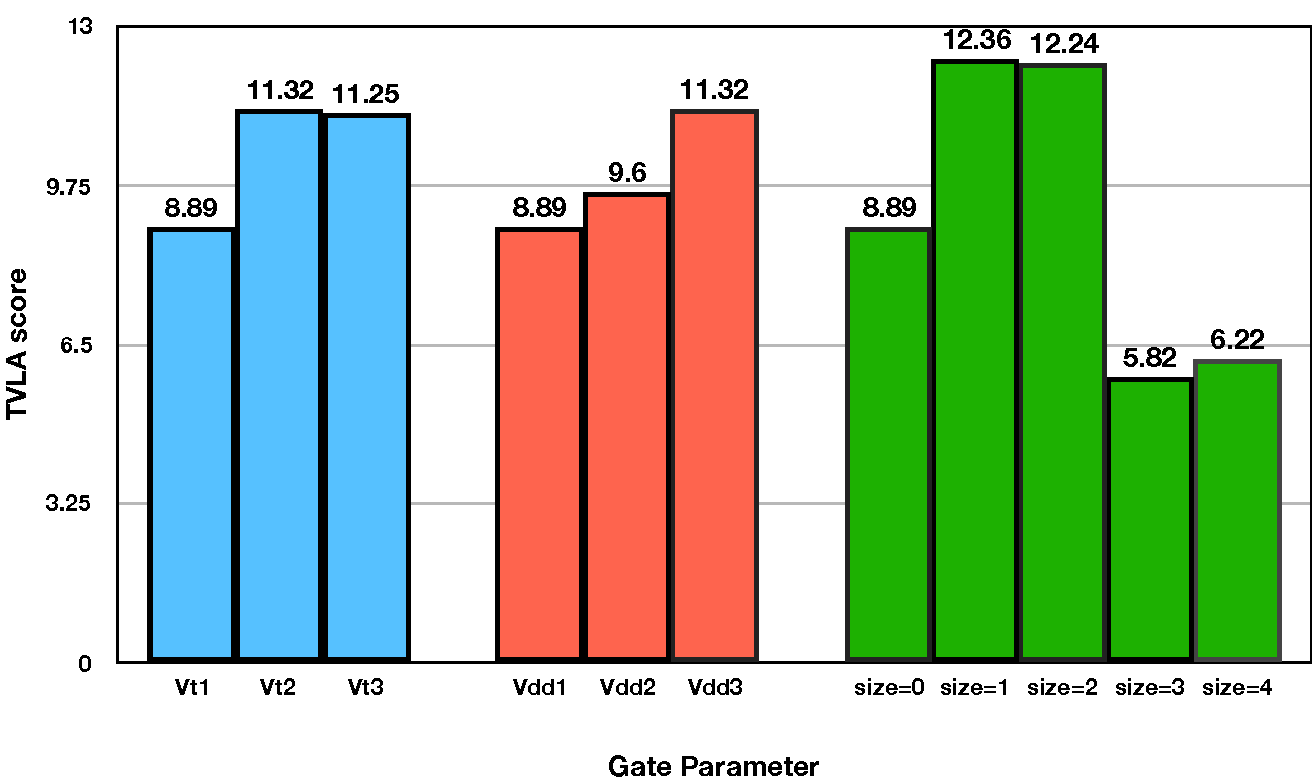
\includegraphics[scale=0.35]{Chapter4/fig/tvla_gate.pdf}
\caption{Variation of TVLA score with $V_{t}$,$V_{dd}$ and $size$ for an AND tree design.}
\label{fig:gateparam}
%\vspace{-15pt}
\end{figure}


% \begin{figure*}[ht!]
% \centering
% \begin{subfigure}{.5\textwidth}
%   \centering
%   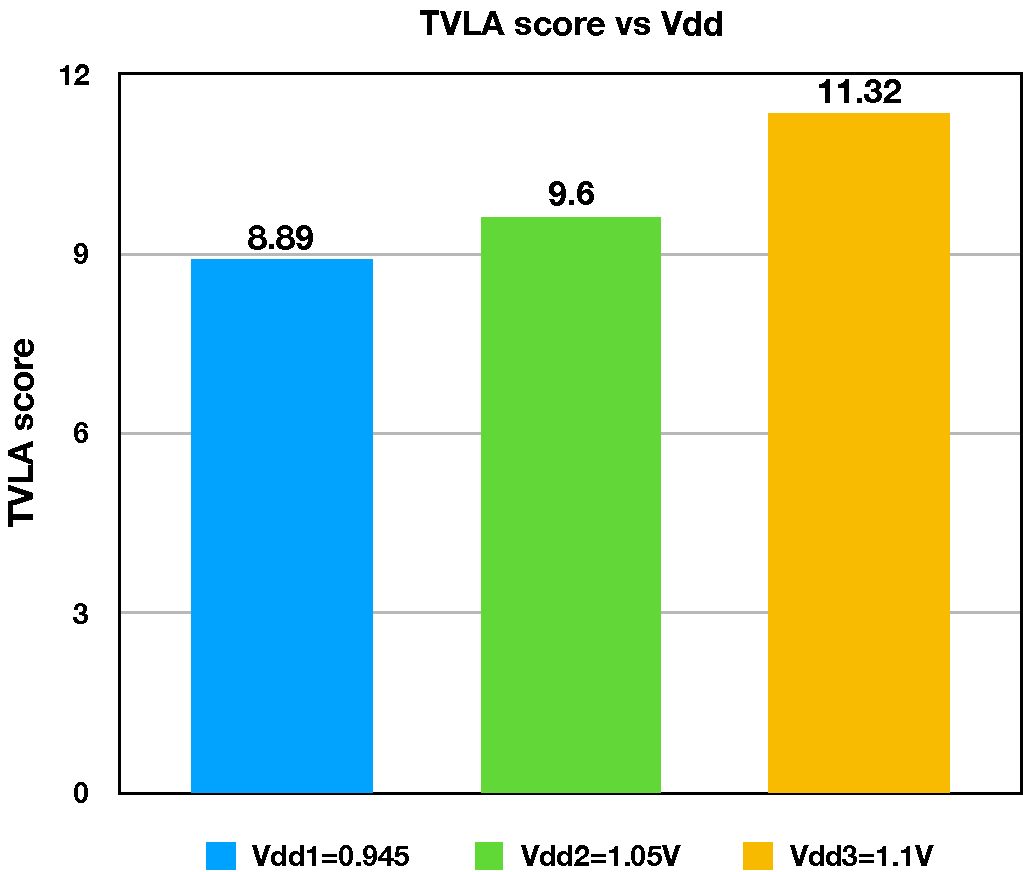
\includegraphics[width=10cm,height=5cm,keepaspectratio]{fig/tvla_vdd.pdf}
%   \caption{Variation of TVLA score with $V_{dd}$.}
%   \label{fig:sub1}
% \end{subfigure}%
% \begin{subfigure}{.55\textwidth}
%   \centering
%   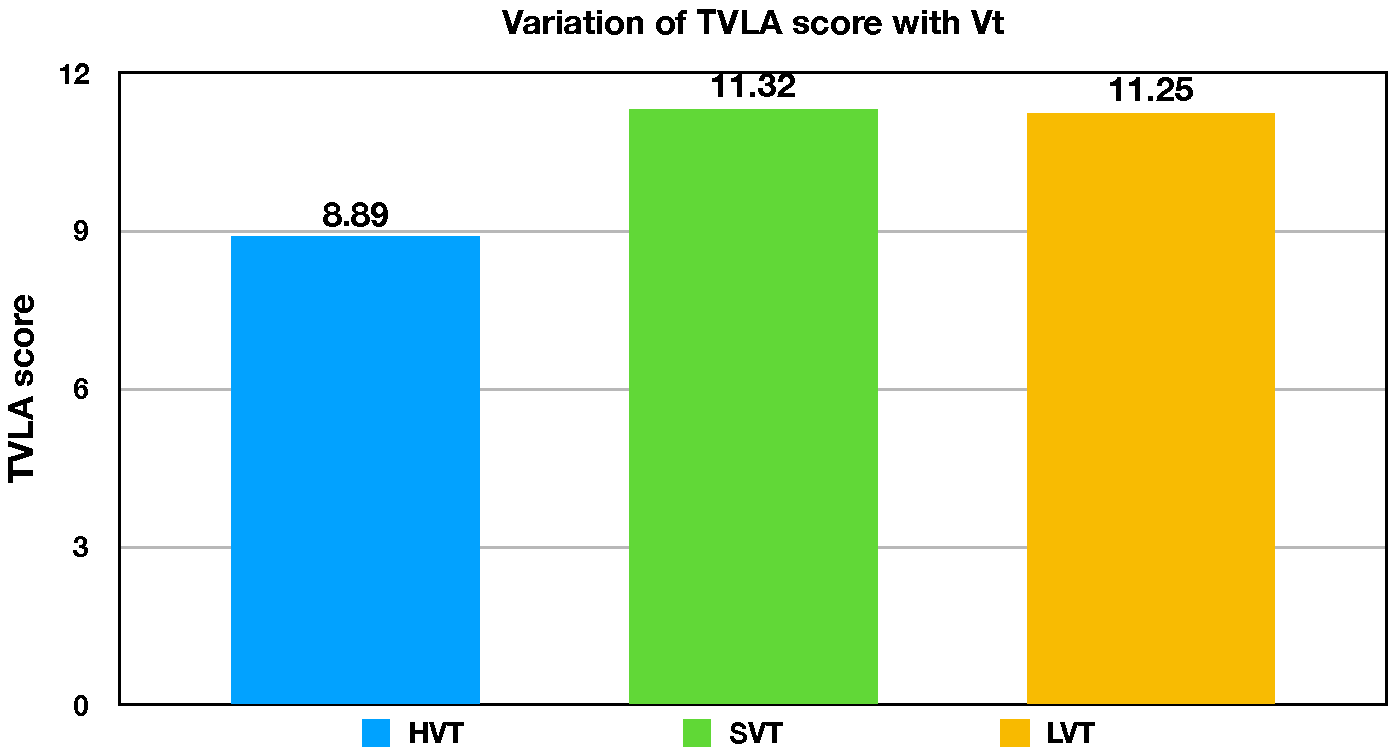
\includegraphics[width=8cm,height=5cm,keepaspectratio]{fig/tvla_vt.pdf}
%   \caption{Variation of TVLA score with $V_{t}$. }
%   \label{fig:sub2}
% \end{subfigure}
% \begin{subfigure}{.75\textwidth}
%   \centering
%   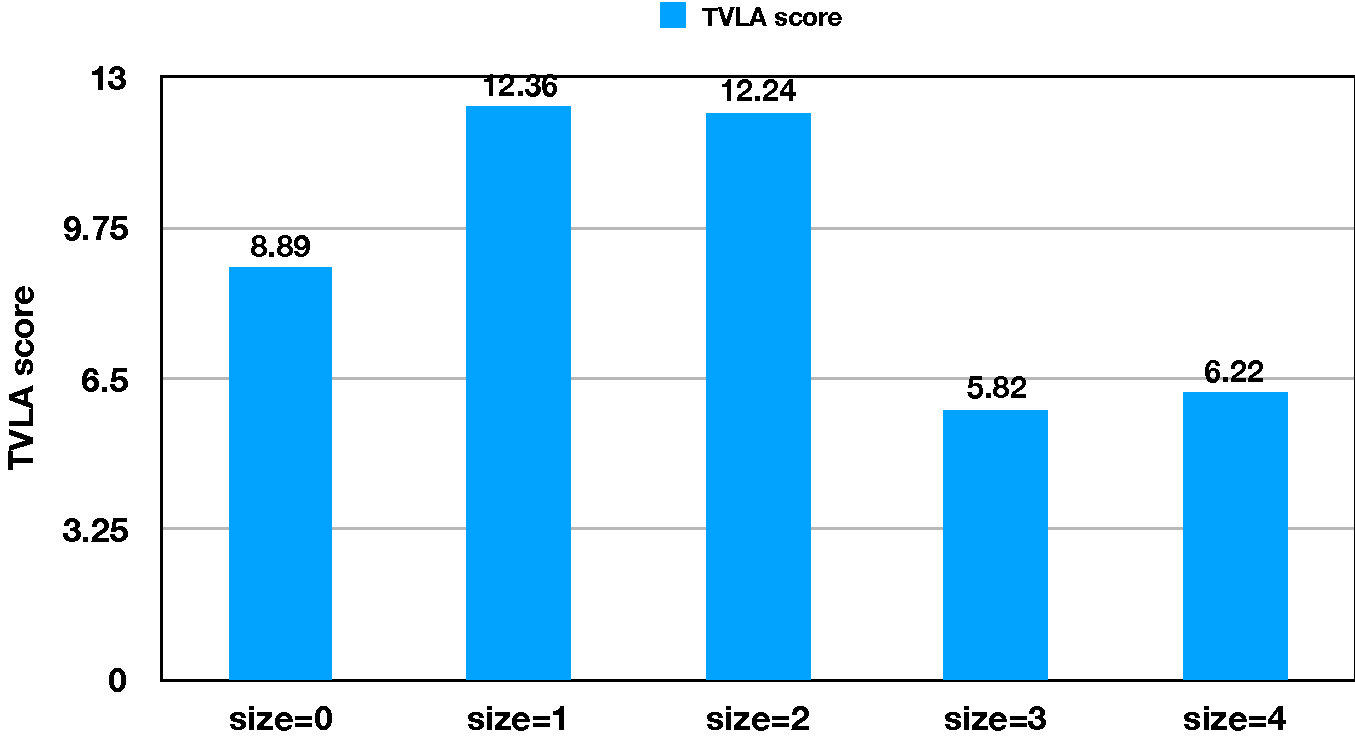
\includegraphics[width=8cm,height=5cm,keepaspectratio]{fig/tvla_size.pdf}
%   \caption{Variation of TVLA score with size. }
%   \label{fig:sub3}
% \end{subfigure}
% % \begin{subfigure}{.75\textwidth}
% %   \centering
% %   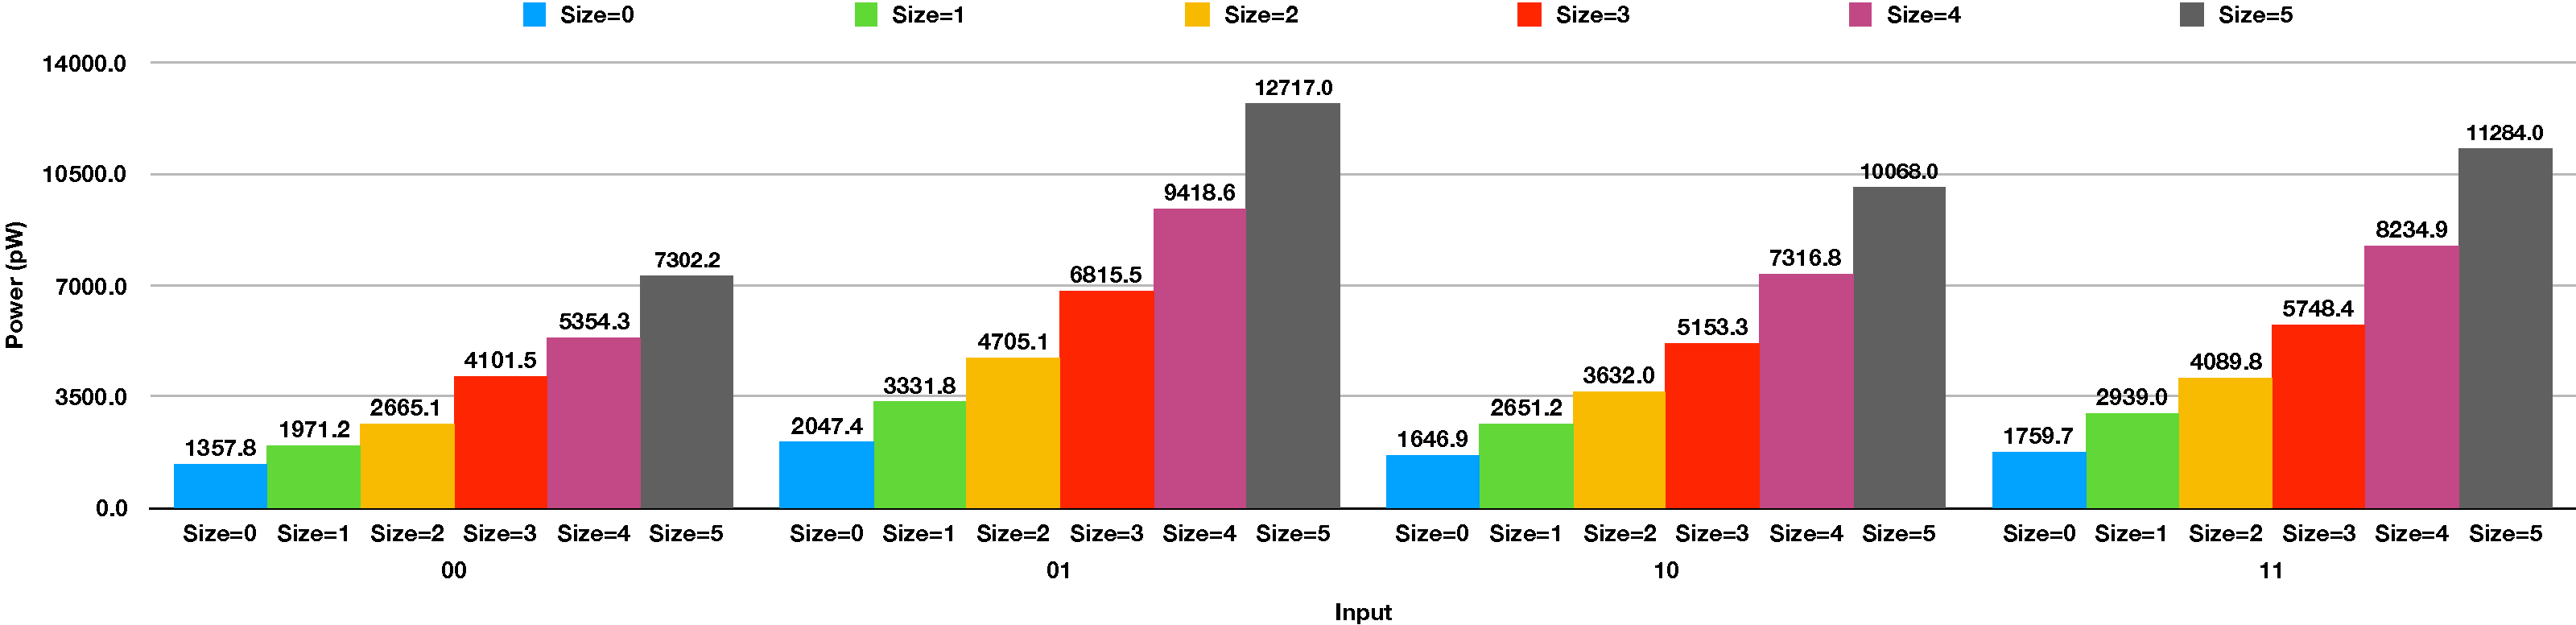
\includegraphics[width=14cm,height=5cm]{fig/sizevsinput.pdf}
% %   \caption{Variation of dynamic power of an AND gate with $size$ and logic level}
% %   \label{fig:sub3}
% % \end{subfigure}%
% % \caption{Figure showing variation of dynamic power of an AND gate with $V_{dd}$, $V_{t}$ and $size$.}
% \label{fig:power}
% \end{figure*}

% \begin{figure*}[ht!]
% \centering
% \begin{subfigure}{.5\textwidth}
%   \centering
%   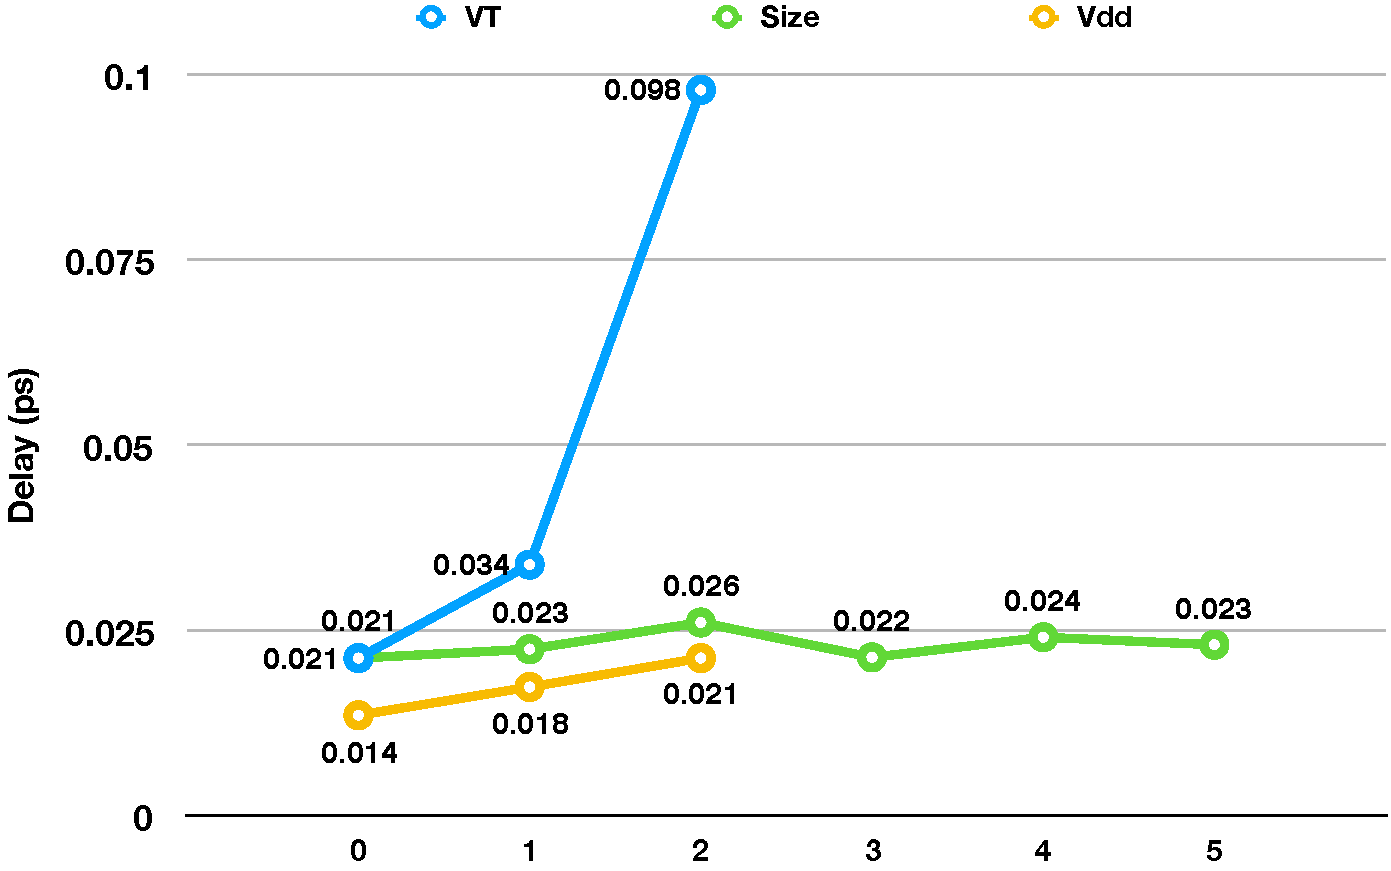
\includegraphics[width=10cm,height=5cm]{fig/delayvariation.pdf}
%   \caption{Variation of delay of an AND gate with $V_{dd}$,$V_{t}$ and $size$.}
%   \label{fig:delay1}
% \end{subfigure}%
% \begin{subfigure}{.55\textwidth}
%   \centering
%   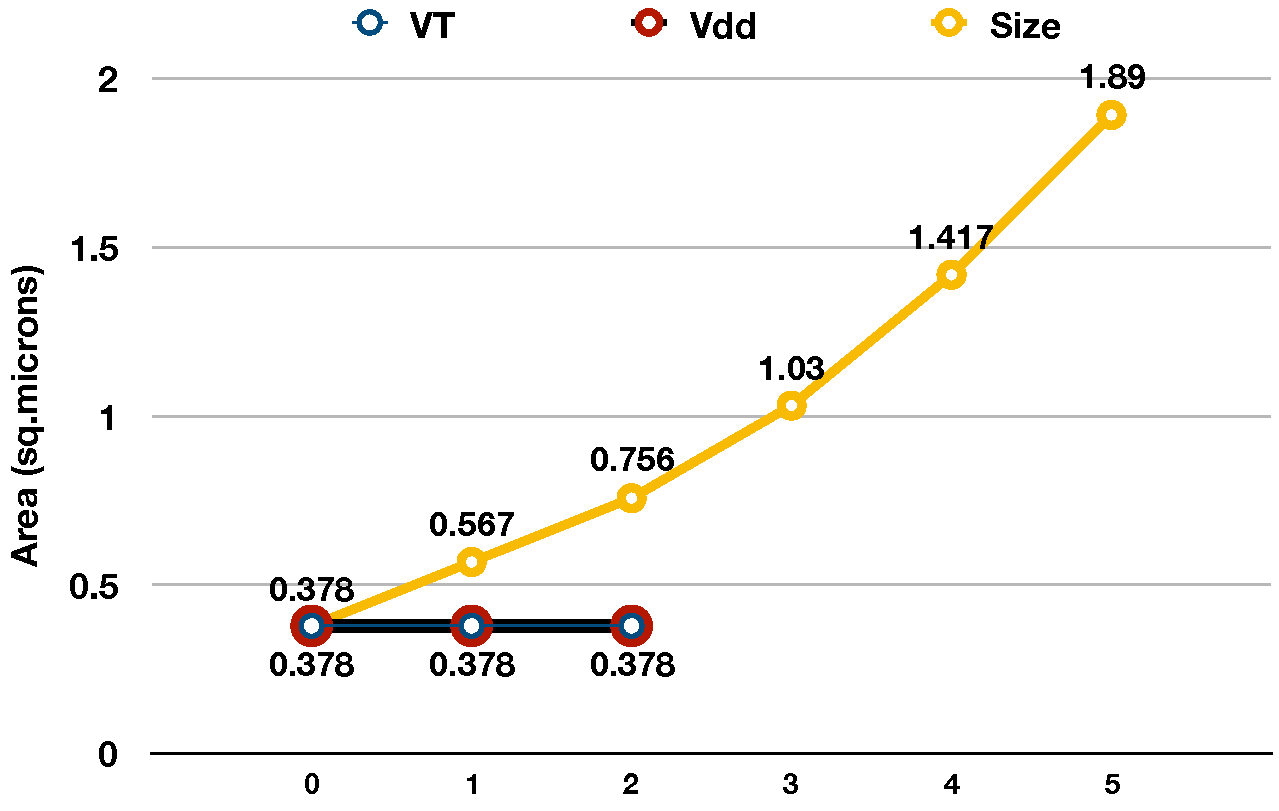
\includegraphics[width=8cm,height=5cm]{fig/areavariation.pdf}
%   \caption{Variation of area of an AND gate with $V_{dd}$, $V_{t}$ and $size$. }
%   \label{fig:delay2}
% \end{subfigure}
% \caption{Figure showing variation of delay and area of an AND with respect to $V_{dd}$, $V_{t}$ and $size$. It can be seen that delay increases with increase in $V_{dd}$, $V_{t}$ and size while area remains constant for $V_{dd}$ and $V_{t}$ scaling and increases with increase in size}
% \label{fig:delay}
% \end{figure*}


\begin{namedthm}{Observation }
Not all regions of the synthesized design contribute equally to the leakage.
\end{namedthm}
{\flushleft There} are certain areas in the design that have a higher leakage compared to other areas. In order to evaluate this, we divided the netlist into a $10 \times 10$ grid and computed the TVLA score for each region independently, thus obtaining 100 different TVLA scores corresponding to various regions in the  netlist. Figure~\ref{fig:aesopt} shows the variations in the TVLA score calculated for netlist III. 
{\sf Karna}, reconfigures the units where leakage is high, so as to reduce the overall side-channel leakage of the design without compromising the other design requirements. 


\begin{namedthm}{Observation }
The side-channel leakage from a gate depends on its  parameters.
\end{namedthm}
In order to observe the impact of each gate configuration on the side-channel leakage, we synthesized an AND-tree design with 16-bit input and 1-bit output, multiple times with different gate configurations. Each synthesis run was done with a different gate configuration. Figure~\ref{fig:gateparam} shows the TVLA scores obtained from 2000 pairs of simulated power traces for each run. It can be seen that changing 
$V_{dd}$, $V_t$ or $size$ options for a gate has an impact on the side-channel leakage of the design.

%Hence, it is important to select gate configurations that meet the design requirements but do not impact the security constraint.
%As mentioned earlier, the EDA tool optimizes the $V_{dd}$, $V_{t}$ and  size of each gate in the design in order to meet a given constraint.We now examine the impact of modifying the design choices by using an AND gate as an example. Figure~\ref{fig:power} shows the variation of dynamic power of an AND gate when the supply voltage $V_{dd}$ and threshold voltage $V_{t}$ are varied. It can be seen that increasing the supply voltage will cause the power consumed by the gate to increase by $\approx5\times-20\times$. We can also observe that the power consumed for different inputs (i.e, $00$, $01$, $10$, and $11$) is different. For example, the difference in the power consumed for inputs $11$ and $01$ at $V_{dd}=1.1V$ is $288$ pW, whereas the difference is $3.5$ pW at $V_{dd}=0.945V$. Such differences can be leveraged to distinguish between the inputs provided at the AND gate and may affect the overall security of the design. A similar observation can be made in figure~\ref{fig:sub2} for $V_{t}$ and figure~\ref{fig:sub3} for varying the gate size. 

A na\"ive approach to achieve security would be to choose gate configurations that provide highest security. However,  na\"ively choosing such gate configurations may violate other design requirements such as delay and power. 
Therefore, there is a need for a careful strategy to vary the gate parameters such that the overall security of the design improves while still meeting the desired design requirements.  
\vspace{-3pt}
% Motivation for post-placement
%It is important to note that the security countermeasures incorporated at any given stage should remain persistent throughout the other stages in the flow. For example, incorporating security at a post-synthesis stage might cause the design to violate area requirements in the placement stage thus requiring re-synthesis. Another consequence is that the tool could optimized out the proposed countermeasures thereby rendering them ineffective. 
%In this work, we therefore choose to introduce the {\sf Karna} module which selects the appropriate gate configuration for each after the design is placed. At this stage, a realistic estimation of the interconnect delay and power density is known. Thus, in this stage, we can accurately gauge the impact of the proposed security based modifications on the area, delay, and performance of the device. 

% a gate $g_{i}$ to be in the critical path of a design iff }




%The problem of securing devices against power side channel attacks has been explored since \cite{} and \cite{}. Techniques like \cite{} and \cite{} have explored software level and device level techniques to address this issue. However, software level techniques only alleviate the symptoms but fail to address the root cause of such vulnerabilities. Device level techniques rely on modifying the physical traits of the device either at gate level as in \cite{}. In this work we explore an alternative idea of mitigating power side-channels at the design level. We motivate the need for such a technique in this section. %This is what disconnected writing gets you, you idiot!

%\indent A power side-channel is said to occur when the device under test consumes drastically different power for a specific input vector than for other random inputs. Mitigating this problem would mean producing a configuration for the device such that it consumes constant or near constant amount of power for any input thereby reducing the statistical variation between the power signature for a fixed input. In device terms this would mean assigning each gate in the device a configuration such that the overall power consumption is fairly constant. 

%\indent In a typical VLSI design flow, the device typically undergoes several optimizations, each with its own objective. The primary of these requirements is performance. The recent power wall and the need for compact devices has led to the emergence of power and area as additional requirements. However, it should be noted that power and area are optimized only if the primary objective is satisfied. 

%\textbf{Observation 1: This drive for a performance optimized design cause the designers to pick gate configurations that, while making the design efficient, might make it compromise the security of the device.}

%It can be seen that while the various algorithms in the EDA flow optimize the design for one or more of performance,area or power, none of them consider the impact on the overall security of the device. This causes the algorithms to pick gate configurations that, while making the design optimal with respect to its requirements, lower the MTD of the device. 





% \indent When we observe the overall power consumption of the device, it can be divided into two components viz. static and dynamic power consumption. Static power is the power that the device consumes during the idle stage and is influenced by temperature, Threshold voltage ($V_t$) and the size of the gate ($g^i_s$). Dynamic power, is the power that is consumed when the device performs some computation, and is affected by the load capacitance ($C_i$), supply voltage $V_(dd)$, and the operating frequency ($F$). It is interesting to see the impact of modifying one or more of these device parameters on the power side-channel of the device.

% \indent Table~\ref{tab2} and~\ref{tab3} shows the leakage power and dynamic power of an inverter. It can be seen that varying $V_t$, $size$, $V_(dd)$ and load capacitance of a gate has an impact on the amount of power that the gate finally consumes. 
% \begin{table}[!ht]
% \begin{tabular}{|c|c|c|c|}
% \hline
% \textbf{Logic Level} & \textbf{$V_{(dd)_1}$} & \textbf{$V_{(dd)_2}$} & \textbf{$V_{(dd)_3}$} \\ \hline
% 00                   &               &               &               \\ \hline
% 01                   &               &               &               \\ \hline
% 10                   &               &               &               \\ \hline
% 11                   &               &               &               \\ \hline
% \end{tabular}
% \label{tab2}
% \caption{Table showing the impact of $V_(dd)$ on the power consumed.}
% \end{table}

% \begin{table}[!ht]
% \begin{tabular}{|c|c|c|c|}
% \hline
% \textbf{Logic Level} & \textbf{$V_{t_1}$} & \textbf{$V_{t_2}$} & \textbf{$V_{t_3}$} \\ \hline
% 00                   &               &               &               \\ \hline
% 01                   &               &               &               \\ \hline
% 10                   &               &               &               \\ \hline
% 11                   &               &               &               \\ \hline
% \end{tabular}
% \label{tab3}
% \caption{Table showing the impact of $V_t$ on the power consumed.}
% \end{table}
% It can be seen that varying $V_t$, $size$, $V_(dd)$ has an impact on the amount of power a gate consumes and thereby it also impacts the power side channel of the entire device. Hence there exists the need for a optimization scheme that takes into account the security of the device. In the next section we introduce Karna, a security aware power optimization scheme.




% %\indent Table~\ref{tab4} shows the various requirements that are addressed during the design manufacturing, it can be noted that security is never viewed as an objective during these stages. This is because quantifying the security or degree of "trust" in a chip is a hard problem to solve in itself. It is harder to quantify the "change" in the degree of trust due to an optimization. Figures~\ref{fig1} and ~\ref{fig2} represent two different optimization choices performed on the same design. It can be seen that 

% %\textbf{Observation 3: There exists a need to reliably quantify the impact of a design optimization on the security of the device.}

% %It can be seen that there exists a need for a design level solution that is able to quantify the impact of design optimizations on security. This will enable designers to explore security aware design optimizations such that performance goals can be achieved while minimizing the vulnerability of the device. In the next section, we will explore how existing metrics can be translated %find a better word
% %into design level requirements and a security aware power minimization scheme. 





\section{Types of Information Feedback}
\label{feed}
In an online sequential setting, the feedback that the learner receives from the environment can be characterized into three broad categories, full information feedback, partial information feedback and bandit feedback. 


    To illustrate the different types of feedback we will take help of the following example. Let a learner be given a set of finite actions $i\in\A$ such that $|\A|=K$. Let, the environment be such that each action has a probability distribution $D_i$ attached to it which is fixed throughout the time horizon $T$. The learning proceeds as follows, at every timestep the learner selects $m\in\A$ actions and observes some form of feedback vector $G^{obs}_{t}$ (which will be characterized later). Before the learner selects the set of arms the environment draws the feedback vector $F^{env}_t\in[0,1]^{K}$ of $K$ i.i.d random rewards for all actions $i\in\A$ from $D_i,\forall i\in\A$ which it decides to reveal in particular format depending on the form of feedback chosen for the game, that is full information, partial information or bandit feedback. This game is shown in algorithm \ref{alg:OSeqGame}. 

% \begin{algorithm}[!th]
% \caption{An online sequential game}
% \label{alg:OSeqGame}
% \begin{algorithmic}
% \State {\bf Input:} Time horizon $T$, $K$ number of arms with unknown parameters of reward distribution
% \State \For{ each timestep $t=1,2,\ldots, T$}
% \State The environment chooses a reward vector $F^{env}_{t}= \left[r_{i,t}\sim^{i.i.d} D_{i},\forall i\in\A\right]$.
% \State The learner chooses $m$ actions such that $m < K$ following some policy $\pi$, where $\A$ is the set of arms and $|\A|=K$.
% \State The learner observes the reward vector $G^{obs}_{t}\subseteq F^{env}_{t}$.
% \State \EndFor
% \end{algorithmic}
% \end{algorithm}

%Let $G(V, E)$ denote a graph where $V$ denotes the set of nodes in the graph and $E$ denotes the set of edges of the graph. Let there be a single starting node, denoted by $\mathcal{s}\in V$ from where the learner must start and try to reach the destination node denoted by $\mathcal{d}\in V$. Each edge has a delay associated with it which is unknown to the learner. This delay is an $i.i.d$ random variable from the distribution $D_{ij}$ associated with the edge $e_{ij}$ between the vertices $v_i$ and $v_j$. Whenever an edge is chosen the environment reveals to the learner  At every timestep the learner chooses a set of edges and receives some form of feedback from the environment. The goal of the learner is to find the path from $s$ to $d$ which has the minimum delay associated with it. 


\subsection{Full Information Feedback}
In full information feedback, when a learner selects $m$ actions then the environment reveals the rewards of all the actions $i\in \A$. Hence, in this form of feedback  the learner observes $G^{obs}_{t} = F^{env}_{t}=[r_{i,t},\forall i\in\A]$. This has been studied in many forms previously in \citet{takimoto2003path}, \citet{kalai2005efficient} or in online prediction with full information feedback in \citet{cesa2006prediction}.


\subsection{Partial Information Feedback}
In partial information feedback, when a learner selects $m$ actions then the environment reveals the rewards of only those $m$ actions for $m\in \A$. Hence, in this form of feedback  the learner observes $G^{obs}_{t} = [ r_{m,t},\forall m\in\A ]$. This is also sometimes called the semi-bandit feedback and has been studied in \citet{awerbuch2004adaptive},   \citet{mcmahan2004online} and \citet{gyorgy2007line}.


\subsection{Bandit Feedback}
In bandit feedback, when a learner selects $m$ actions then the environment reveals a cumulative reward of those $m$ actions for $m\in \A$. Hence, in this form of feedback  the learner observes $G^{obs}_{t} = \sum_{q=1}^{m} r_{q,t}$. Note, that when $m=1$, then the learner observes the reward of only that action that it has chosen out of $K$ actions. Bandit feedback for single action has been extensively studied in literature with many open problems and we focus on its various interpretations in this thesis.



\section{Different types of Bandits}
\label{types}
\input{Chapter1/types}


\section{Objectives of Thesis}
\label{objThesis}
The main objectives of the thesis are as follows:-
\begin{enumerate}
\item The first objective of this thesis is to study the impact of gate-sizing on leakage power minimization. Our problem formulation takes into account the delay constraints of a given design. We also address the issues of scalability and, runtime.

\item The second objective of this thesis is to study the impact of gate-sizing as a possible countermeasure for power side-channel attacks. We propose a gate-sizing algorithm whose objective is to minimize information leakage via the power side-channel. We analyze the effectiveness of this algorithm by employing three different cipher designs. We also discuss the various factors affecting the convergence of the 
%area of thresholding bandit problem (TBP) setting where the goal is to minimize the expected loss at the end of a fixed budget provided as input. We intend to provide strong guarantees with respect to expected loss and also propose the algorithm that does not require any problem complexity as an input. We also intend to provide strong empirical evaluations of the algorithm proposed for the TBP setting.

%\item The third objective of this thesis is to study the area of piecewise stochastic bandit where again the goal is to minimize the cumulative regret. We intend to provide strong algorithms that can adapt to this environment and performs well empirically.  
\end{enumerate}

\section{Contributions of Thesis}
\label{contriThesis}
The main contributions of the thesis are as follows:-
\begin{enumerate}
\item We propose the MLTimer alogrithm that uses gate-sizing for reducing the leakage power consumption of a digital design. We propose a smart one-pass tool that can leverage the right optimization technique at the appropriate stage of the flow thereby improving design productivity. A key observation reported in MLTimer is that there exists significant correlation between the timing slacks of gates in the current iteration to the gate replacements in successive iterations. MLTimer leverages this observation to reduce the number of STA runs thereby reducing the overall time taken for optimization.

\item We propose the Karna algorithm which uses gate-sizing for reducing the information leakage via the power side-channel of a digital design. We show that each region in a given design leaks information differently. Thus, it is sufficient to optimize gates in the highly sensitive regions to reduce information leakage. Karna leverages this observation and optimizes gates in these sensitive regions to reduce the power side-channel vulnerability. 

%\item We proposed a general framework of bandit algorithms that combines change-point detection algorithm with aggregation of expert strategies in order to define efficient pulling strategies in the context of the piecewise stochastic distributions. The algorithms that we proposed for the piecewise stochastic setting are actively adaptive algorithms which perform very similarly to the oracle algorithm which has access to the changepoints and suffers no additional delay in adapting to the changing environment. 
\end{enumerate}
 

\section{Outline of the Thesis}
\label{outline}
 In this chapter, we gave an overview of the power and security issues in digital designs. We also discussed the gate-sizing technique and its role in solving the above two problems. We now outline the general structure of this thesis. In the next chapter, we discuss MLTimer, a learning based lazy evaluation model that uses gate-sizing for solving the leakage power minimization problem in digital circuits. We discuss Karna, a gate-sizing algorithm for reducing the power side-channels in digital designs in Chapter 3. We compare these two schemes in Chapter 4. We conclude by briefly summarizing the problems covered in this thesis and highlight some interesting future directions that they could be further extended.


% various types of bandits available in the literature and also discussed about the main objectives of the thesis and our contributions. In this section, we give a general outline of the thesis that is to follow. In Chapter \ref{chap:SMAB} we give a detailed overview of the stochastic multi-armed bandit model and the latest available algorithms in this setting. In the next Chapter \ref{chap:EUCBV} we introduce our algorithm Efficient UCB Variance (EUCBV) for the stochastic multi-armed bandit model. We give theoretical guarantees on the performance of EUCBV and also show in numerical simulations that it indeed performs very well as compared to the state-of-the-art algorithms. In the subsequent Chapter \ref{chap:tbandit1} we introduce a new variant of pure exploration multi-armed stochastic bandit called the thresholding bandit problem. We analyze the connections between thresholding bandit problem and pure exploration problem and also discuss several existing algorithms in both the settings that are relevant to carefully analyze the thresholding bandit problem. Then in Chapter \ref{chap:tbandit2} we introduce our solution for the thresholding bandit problem, called the Augmented UCB (AugUCB) algorithm. We analyze our algorithm AugUCB and derive theoretical guarantees for it as well as show in numerical experiments that it indeed outperforms several state-of-the-art algorithms in the thresholding bandit setting. Finally, in Chapter \ref{ThesisConc} we conclude by briefly summarizing all the problems covered in the thesis and discussing some future directions in which the stated problems can be further extended.


%Finally, in chapter \ref{chap:psbandit} we introduce the piecewise-stochastic bandit model which is a new variant that strides between the stochastic and adversarial setting. We discuss extensively on this setting and also provide our solution to this setting and show in numerical simulations that our solution is very close to the optimal solution. 


%%%%%%%%%%%%%%%%%%%%%%%%%%%%%%%%%%%%%%%%%%%%%%%%%%%%%%%%%%%%

%%%%%%%%%%%%%%%%%%%%%%%%%%%%%%%%%%%%%%%%%%%%%%%%%%%%%%%%%%%%
\clearemptydoublepage
% \chapter{Stochastic Multi-armed Bandits}
% \label{chap:SMAB}

% \section{Introduction to SMAB}
% \label{sec:intro}
% One of the significant moments that has shaped human history was the invention of the computer. What essentially started out as an attempt to replace and replicate simple arithmetic functions now surrounds us on a day-to-day basis taking care of our transport, health, finance and ingratiating itself into our daily lives more and more. 

This evolution has largely been made possible due to the invention of the transistor by Bell & Schokley in 1951 which caused computers to go from the size of an airplane hangar to tiny microscopic devices.  The invention of the transistors enabled chip designers to meet the ever increasing user requirements by halving the size of the transistors and thereby doubling the number of transistors that could be packed into the same area. This phenomenon also dubbed as Moore’s law has enabled chip designers meet the exponentially increasing functionality requirements.

In addition to increasing functionality, digital devices are also expected to meet additional constraints which can be enumerated using the tuple {Power, Area and Delay}. Depending on the platform in which it gets deployed, the chip designer might have to optimize the same design to meet  two orthogonal constraints. For example, when building a server, the processor is expected to be fast while the power and area requirements are relaxed but on the other hand if the same processor is to be used on a IoT device, the designer might have to optimise the design for low power, smaller area while the device might not be expected to perform at the same speed as the server. **{ Can we rewrite it with a better example?}

We now discuss the three key objectives that a given digital design is expected to meet. 
\begin{enumerate}
    \item \textbf{Delay} With each passing generation 
\end{enumerate}





%Computers have evolved from being simple calculators to devices that can perform complex operations that are employed in various aspects of our day-to-day lives.  
%This evolution has been 

%For the last 70 years, chip designers have been able to meet this expectation by leveraging Moore's law and adding more transistors.  

%Today digital devices can be broadly classified into three different classes \begin{enumerate}
 %   \item Embedded devices: These devices are expected to interact with various aspects of a user's environment such as temperature, motion etc. and make decisions on the fly. The emergence of Internet of Things as a popular networking paradigm in the last 3 years has led to an increase in the demand for such devices. These class of devices typically application specific and perform either "send and send" or lightweight computation at the
%\end{enumerate}

%In this evolution, the expectations of the end-user from each generation has been increasing. While initial generations were expected to merely speed-up arithmetic operations, the development of commercial compute devices starting with Intel's 4004 processor has led to these devices perform complex mathematical functions at a faster rate, on a smaller device by using a little energy as possible. 












% In today's world, artificial intelligence has proved to be a game-changer in designing agents that interact with an evolving environment and make decisions on the fly. The main goal of artificial intelligence is to design artificial agents that make dynamic decisions in an evolving environment. In pursuit of these, the agent can be thought of as making a series of sequential decisions by interacting with the dynamic environment which provides it with some sort of feedback after every decision which the agent incorporates into its decision-making strategy to formulate the next decision to be made. A large number of problems in science and engineering, robotics and game playing, resource management, financial portfolio management, medical treatment design, ad placement, website optimization and packet routing can be modeled as sequential decision-making under uncertainty. Many of these real-world interesting
% sequential decision-making problems can be formulated as reinforcement learning (RL) problems (\citep{bertsekas1996neuro}, \citep{sutton1998reinforcement}). In an RL problem, an agent interacts with a dynamic, stochastic, and unknown environment, with the goal of finding an action-selection strategy or policy that optimizes some long-term performance measure. Every time when the agent interacts with the environment it receives a signal/reward from the environment based on which it modifies its policy. The agent learns to optimize the choice of actions over several time steps which is learned from the sequences of data that it receives from the environment. This is the crux of online sequential learning. 

%     This is in contrast to supervised learning methods that deal with labeled data which are independently and identically distributed (i.i.d.) samples from the considered domain and train some classifier on the entire training dataset to learn the pattern of this distribution to predict the labels of future samples (test dataset) with the assumption that it is sampled from the same domain. In contrast to this, an RL agent learns from the samples that are collected from the trajectories generated by its sequential interaction with the system. For an RL agent, the trajectory consists of a series of sequential interactions whereby it transitions from one state to another following some dynamics intrinsic to the environment while collecting the reward till some stopping condition is reached. This is known as an episode. Here, for an action $i_t$ taken by the agent at the $t$-th timestep, the agent transitions from its current state denoted by $S_{i,t}$ to state $S_{i,t+1}$ and observes the reward $X_{i,t}$. An illustrative image depicting the reinforcement learning scenario is shown in Figure \ref{fig:rl}.

% \begin{figure}[!th]
% \includegraphics[scale=0.45]{Chapter1/img/RL1.png}
% \caption{Reinforcement Learning}
% \label{fig:rl}
% \end{figure}


    
    
% %To express an RL problem more formally, we have to define the idea of Markov Decision Process (MDP) which consists of states, actions, transition probabilities, and rewards which in turn helps in deciding the strategy to be followed by the agent. 

% %An MDP consists of states


% \section{Notations and assumptions}
% \label{sec:notations}
% \input{Chapter2/notation}

% \section{Problem Definition}
% \label{sec:probDef}
% \input{Chapter2/probDef}

% \section{Motivation}
% \label{sec:motivation}
% \section{Motivation for Integrating Security requirements into an EDA Flow}
\label{sec:motivation}

%In this section, we provide a concrete example that highlights the fact that existing EDA optimizations indeed have an effect on the security of the device. 
%need for a security-aware EDA flow that optimizes security along with the typical requirements. We take an AES-128 design and synthesize it to generate six different netlists each of which is optimized to meet a different objective such as low power, high performance \& smaller area, low power \& smaller area, and high performance \& low power. % as shown in Table~\ref{tab:design}. 
%The design configurations with their area, delay, and power numbers are shown in Table~\ref{tab:design}. We then analyze the side-channel resistance of each netlist using the Mean Traces to Leak (MTL) metric defined in Section~\ref{}. %The number of power traces needed to guess the key, called mean time for disclosure (MTD), is shown in the fourth column of Table~\ref{tab:design}. A higher MTD value indicates that the attacker needs to collect large number of samples in order to guess the AES key and a smaller MTD value indicates that the device can be easily exploited via the power side-channel.

% \todo[inline]{table 1 hardly makes sense! out of 6 designs on the 3rd one actually serves the purpose.}
\begin{table}[t!]
\scriptsize
\centering

\caption{Impact of design requirements on Area, Power, Delay and the magnitude of TVLA score at the end of 4000 traces for an AES design.  }
\begin{tabular}{|c|c|c|c|c|c|}

\hline

\textbf{\begin{tabular}[c]{@{}c@{}}Design \\ Choices\end{tabular}} & \textbf{Area} & \textbf{\begin{tabular}[c]{@{}c@{}}Delay \\ (ns)\end{tabular}} & \textbf{\begin{tabular}[c]{@{}c@{}}Static\\  Power ($\mu W$)\end{tabular}} & \textbf{TVLA}\\ \hline
I -- Area $\downarrow$ Power $\downarrow$ &       78883        &                  0.48                                              &                            492.4                                  & 11.077                                                                          \\ \hline
II  -- Area $\downarrow$        &        58439       &                 0.48                                               &    602.42             &  11.41                                                                                                            \\ \hline
III -- Area $\downarrow$ Delay $\downarrow$      &       82545        &               0.47                                                 &    513.40               & 8.22  \\ \hline
IV -- Power $\downarrow$ Delay $\downarrow$     &     102256          &             0.47                                                   &               683.41     & 10.65 \\ \hline
V --    Power $\downarrow$ &    79097           &             0.48                                                   &     482.80              &   9.95\\ \hline
VI -- Delay $\downarrow$    &        91822       &        0.32                                                        &     2105.8                  &  13.97       

\\ \hline

\end{tabular}
\label{tab:design}
\end{table}
\begin{figure}[t!]
\centering
  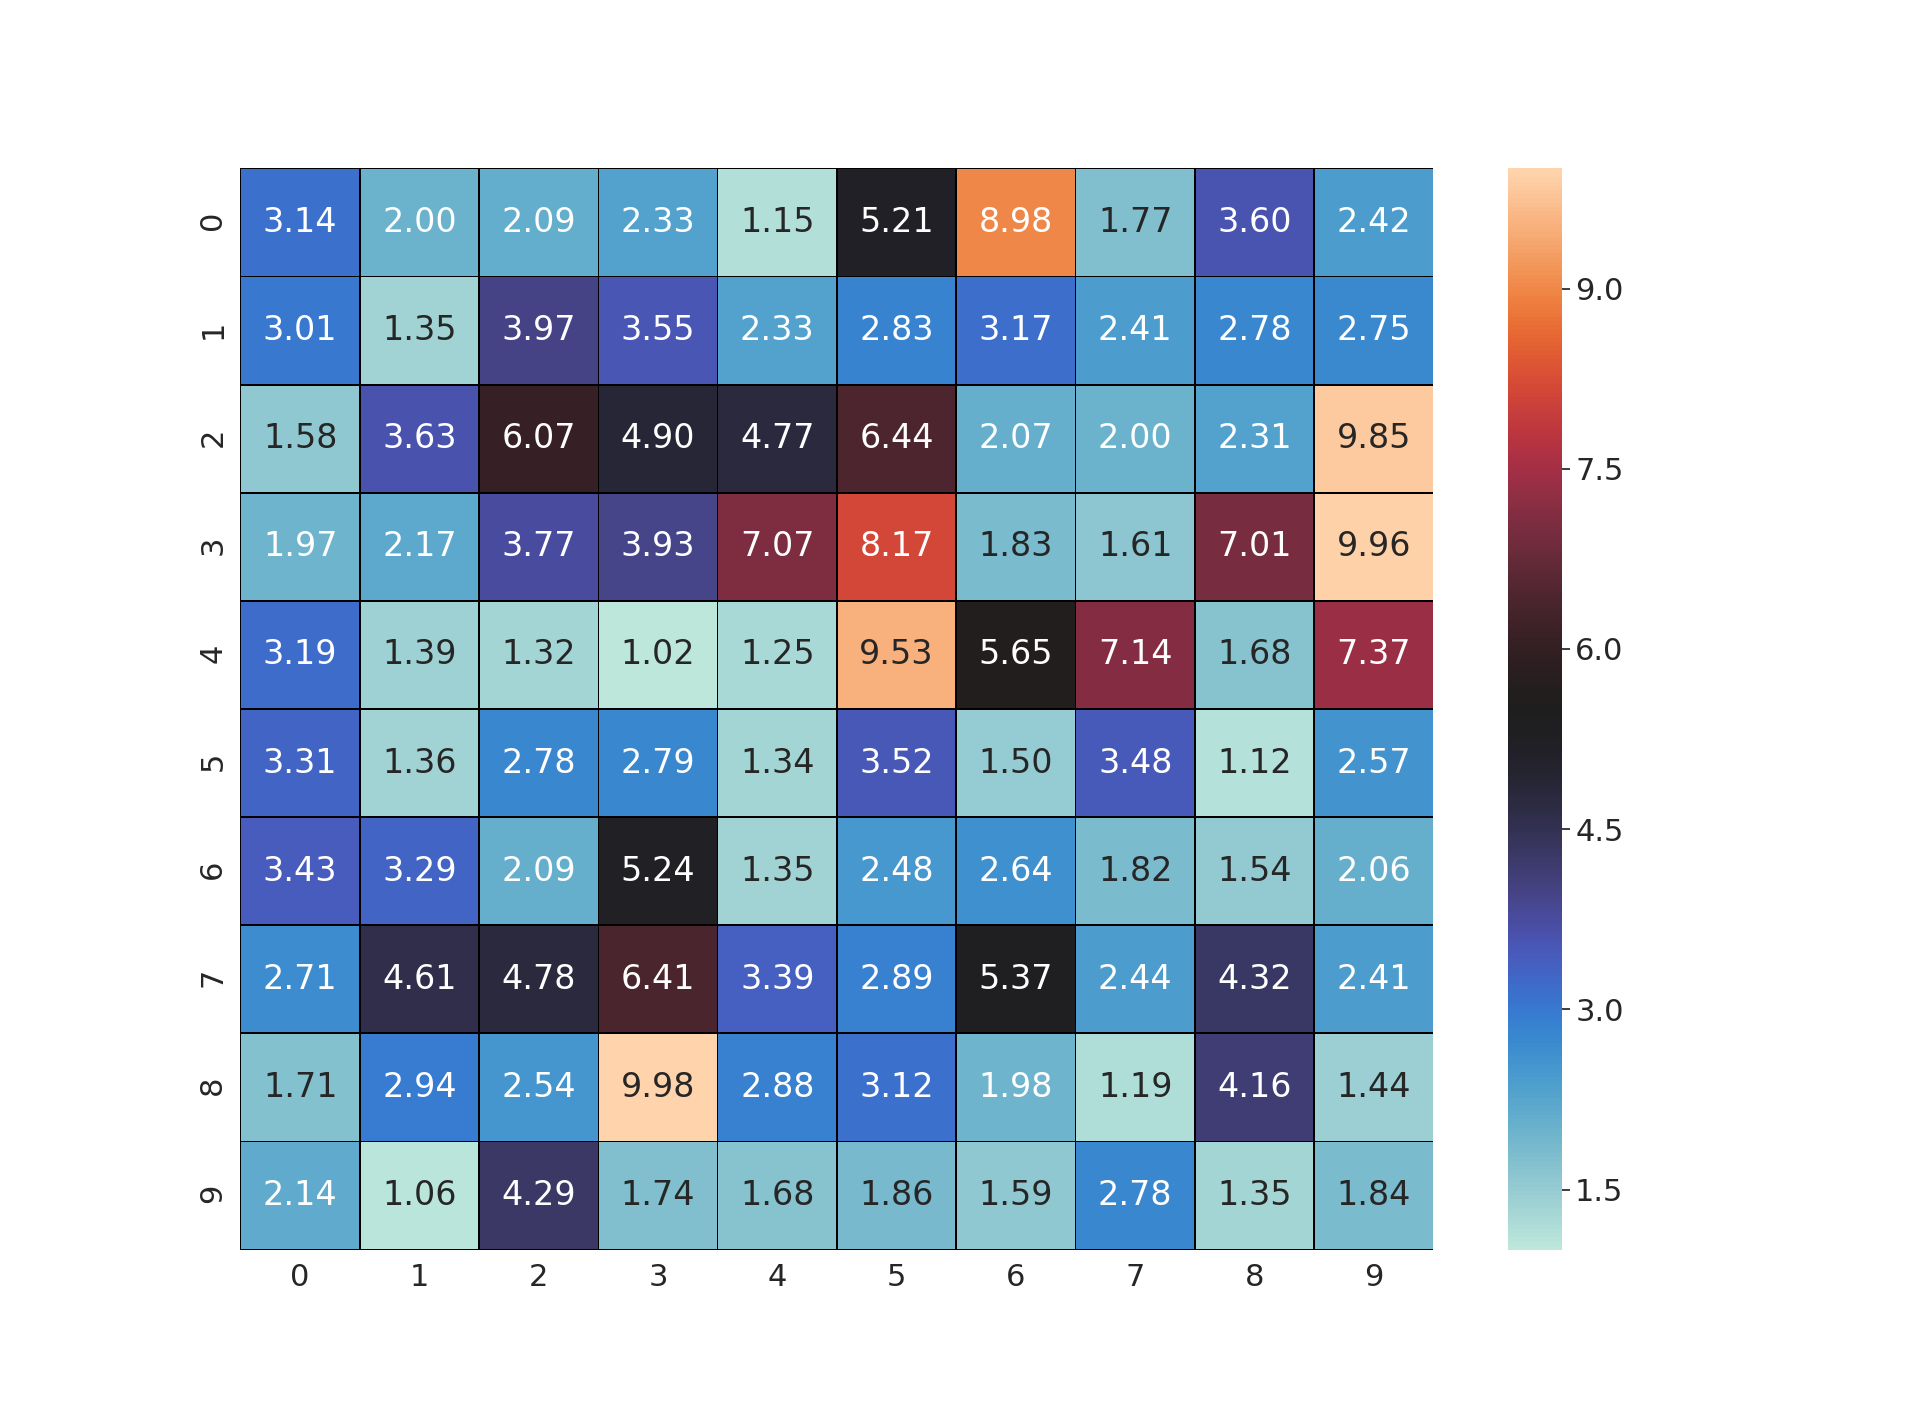
\includegraphics[scale=0.20]{Chapter4/fig/aes_before.png}  
\caption{The TVLA profile of the AES design, with the design divided into a $10\times 10$ grid and the TVLA score of each cell calculated independently. Of the 100 cells, 21 have a TVLA score greater than 4.5. The overall TVLA score of the netlist is 8.22. }
\label{fig:aesopt}
\end{figure}

In this section, we use three critical observations to motivate the use of EDA tools to achieve side-channel security.

\begin{namedthm}{Observation}
EDA algorithms influence the side-channel security of a design.
\end{namedthm}

{\flushleft We} synthesized an AES cipher to meet various design objectives. Table~\ref{tab:design} shows the area, delay, power, and security (TVLA score) of six (I to VI) different netlists. Each netlist was synthesized using the same AES design and used the same EDA tool (Synopsis Design Compiler). The EDA tool was configured with different design requirements for each synthesis. For example, netlist II was synthesized with the objective to reduce area, while netlist IV was synthesized to reduce both power and delay.
For each design, we computed the TVLA score from 4000 pairs of simulated power traces. As seen in the table, we obtain different TVLA scores for each netlist. We thus conclude that design requirements used by an EDA tool have an impact on the overall security of the final device. This experiment corroborates the observations made in~\cite{Verbauwhede:2005, danger:2017, yang:2005}. 
\begin{figure}[t!]
\centering
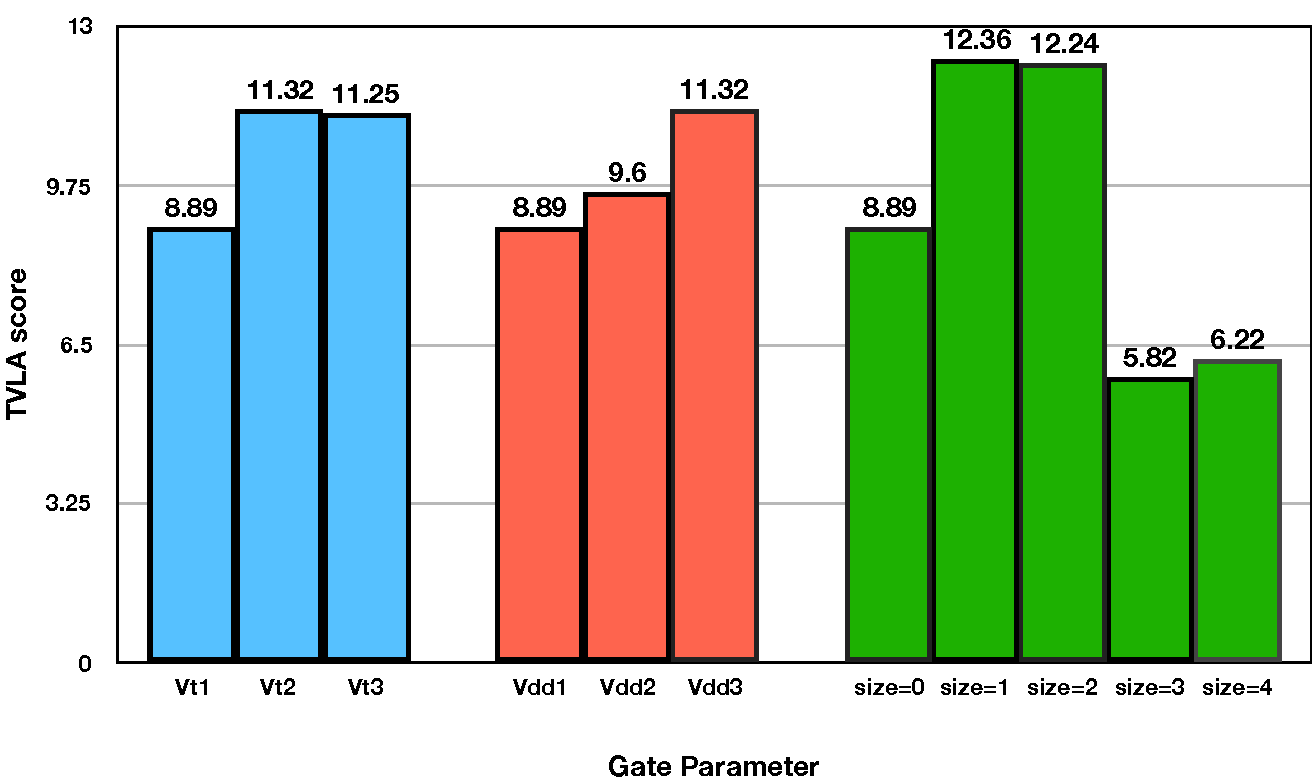
\includegraphics[scale=0.35]{Chapter4/fig/tvla_gate.pdf}
\caption{Variation of TVLA score with $V_{t}$,$V_{dd}$ and $size$ for an AND tree design.}
\label{fig:gateparam}
%\vspace{-15pt}
\end{figure}


% \begin{figure*}[ht!]
% \centering
% \begin{subfigure}{.5\textwidth}
%   \centering
%   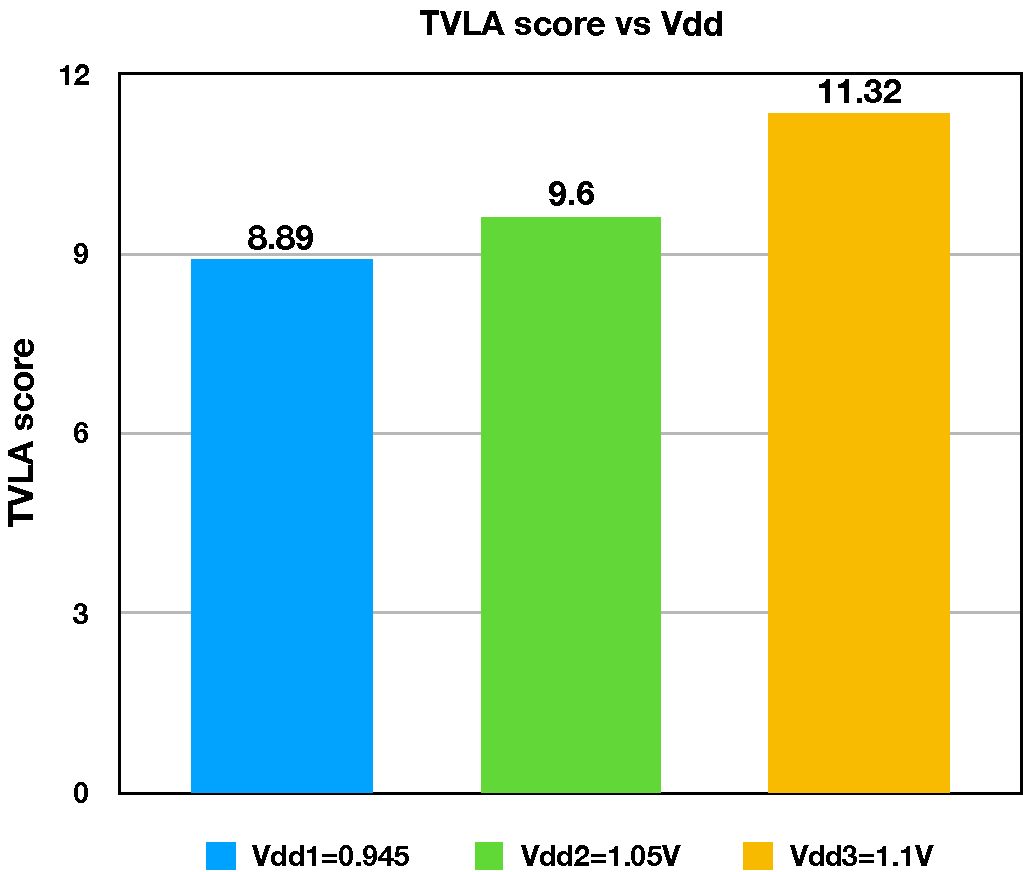
\includegraphics[width=10cm,height=5cm,keepaspectratio]{fig/tvla_vdd.pdf}
%   \caption{Variation of TVLA score with $V_{dd}$.}
%   \label{fig:sub1}
% \end{subfigure}%
% \begin{subfigure}{.55\textwidth}
%   \centering
%   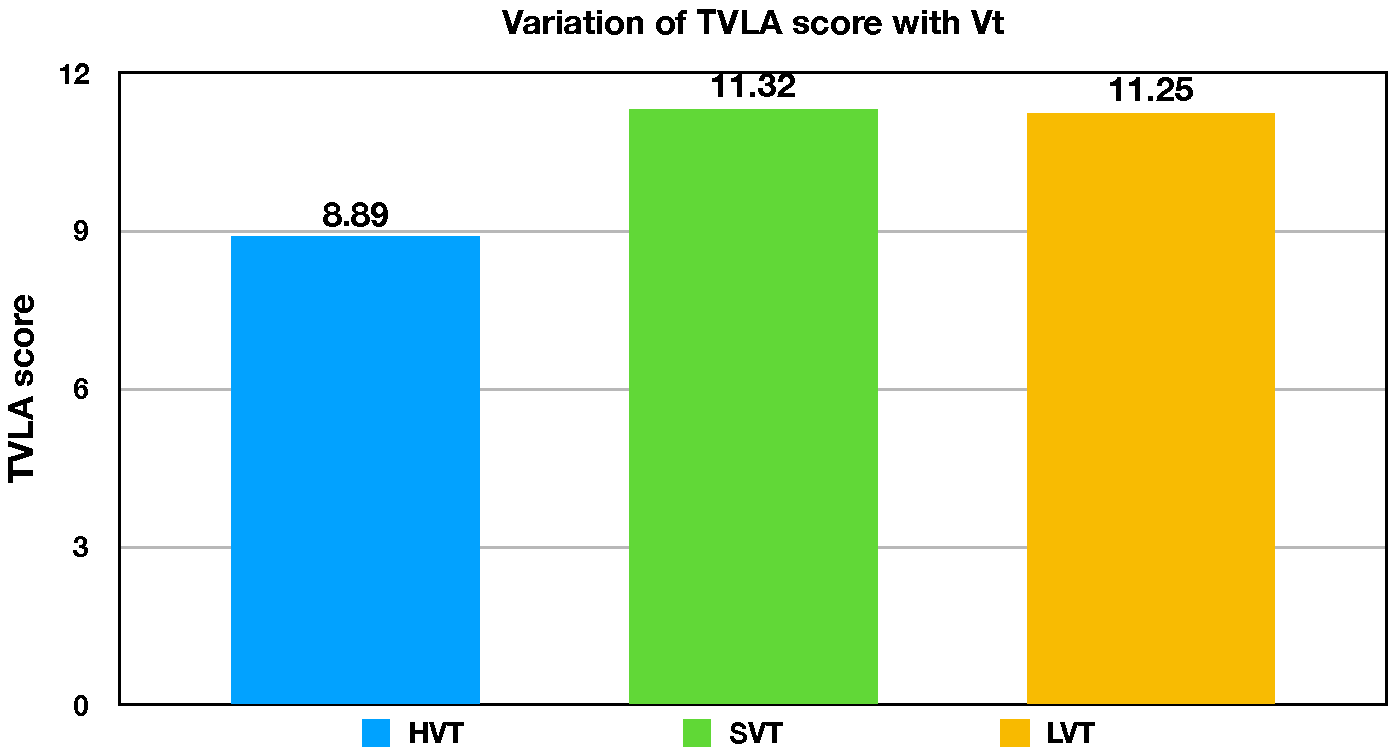
\includegraphics[width=8cm,height=5cm,keepaspectratio]{fig/tvla_vt.pdf}
%   \caption{Variation of TVLA score with $V_{t}$. }
%   \label{fig:sub2}
% \end{subfigure}
% \begin{subfigure}{.75\textwidth}
%   \centering
%   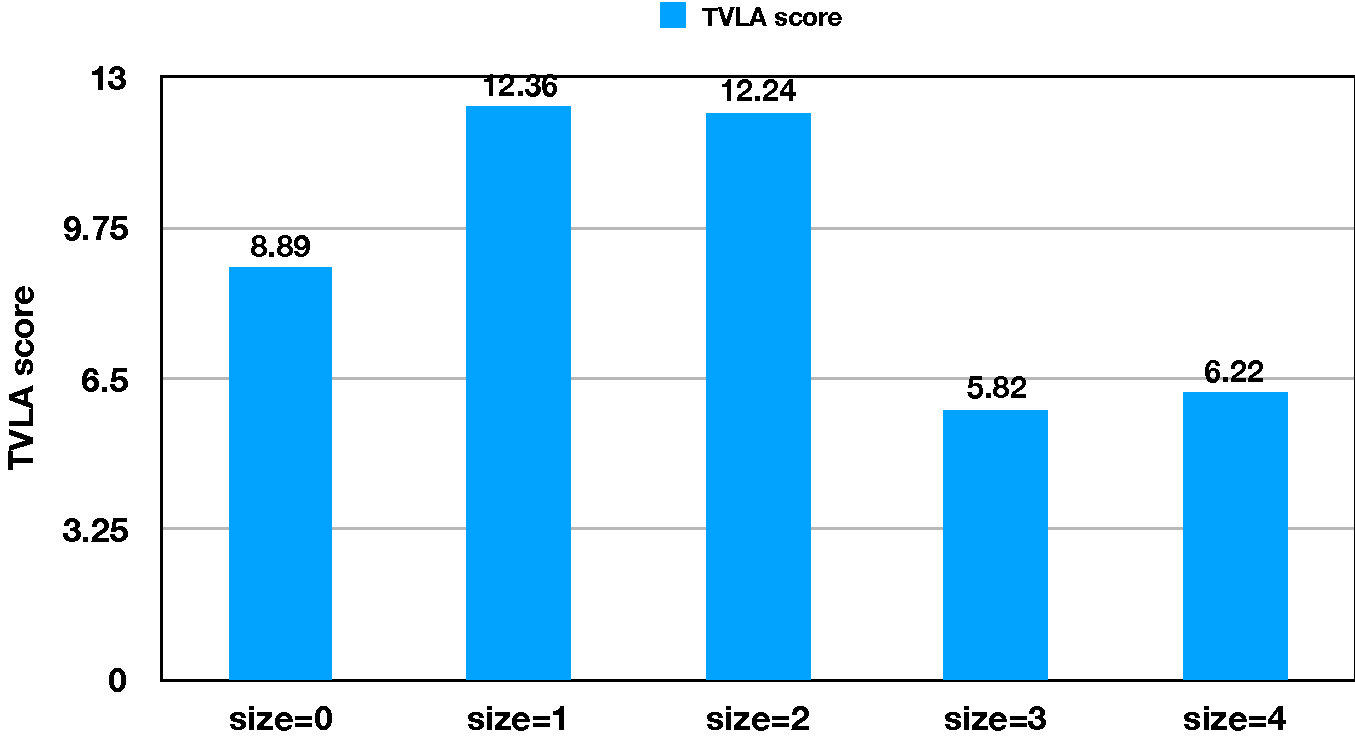
\includegraphics[width=8cm,height=5cm,keepaspectratio]{fig/tvla_size.pdf}
%   \caption{Variation of TVLA score with size. }
%   \label{fig:sub3}
% \end{subfigure}
% % \begin{subfigure}{.75\textwidth}
% %   \centering
% %   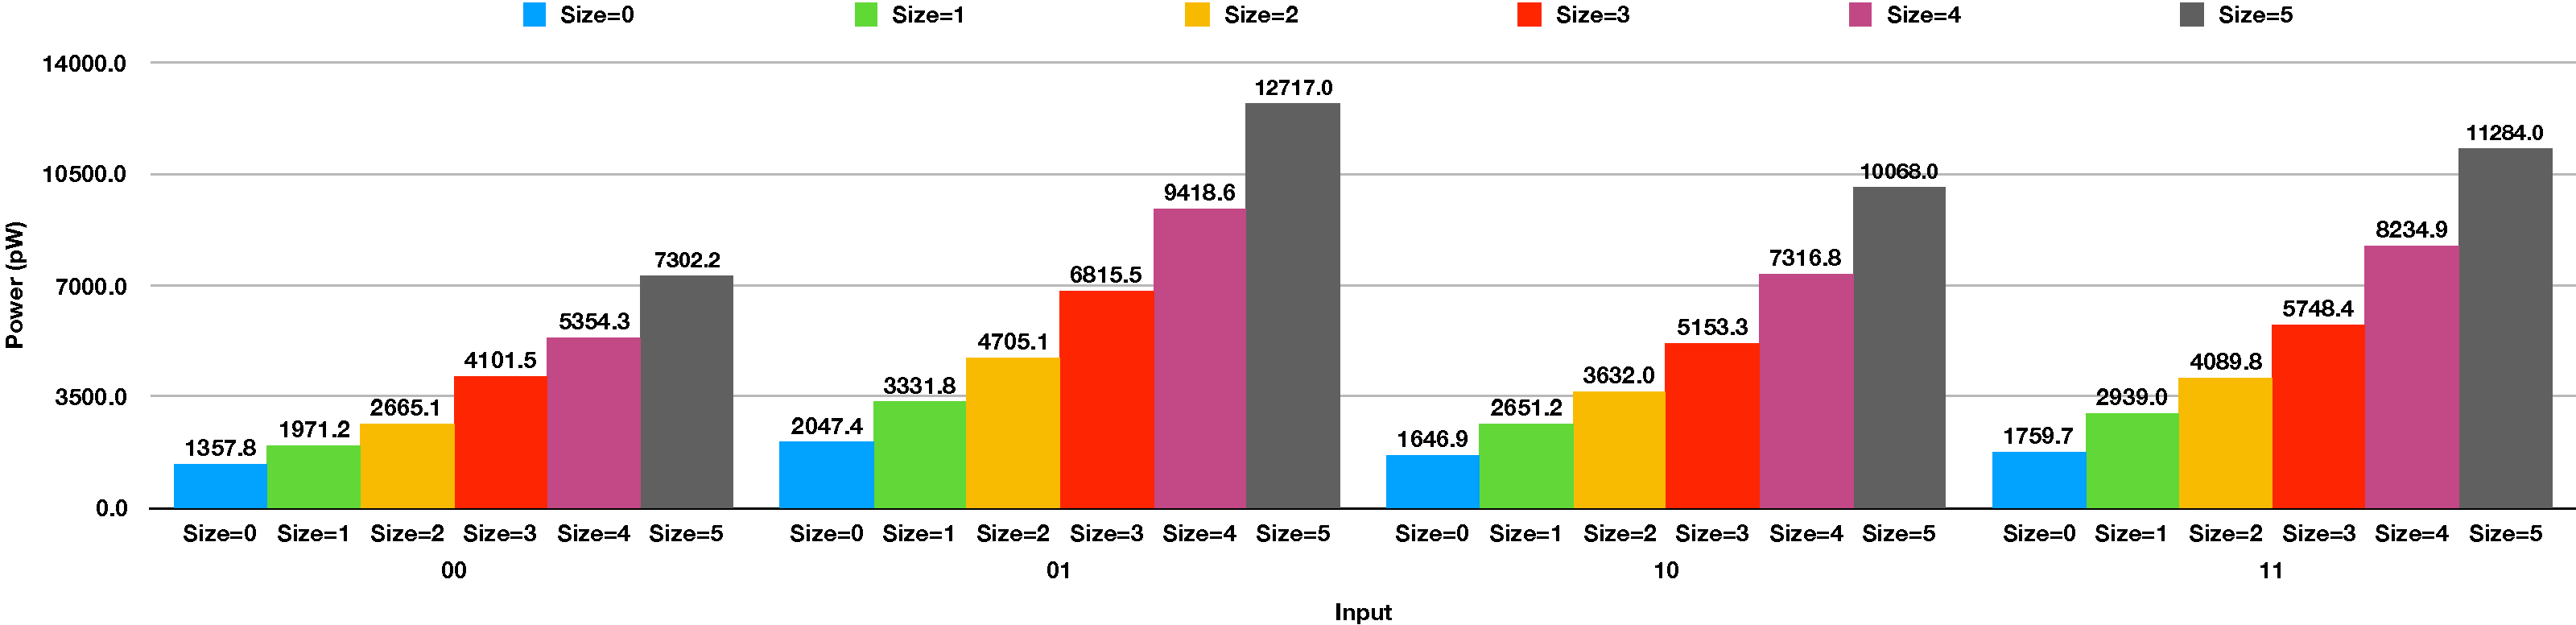
\includegraphics[width=14cm,height=5cm]{fig/sizevsinput.pdf}
% %   \caption{Variation of dynamic power of an AND gate with $size$ and logic level}
% %   \label{fig:sub3}
% % \end{subfigure}%
% % \caption{Figure showing variation of dynamic power of an AND gate with $V_{dd}$, $V_{t}$ and $size$.}
% \label{fig:power}
% \end{figure*}

% \begin{figure*}[ht!]
% \centering
% \begin{subfigure}{.5\textwidth}
%   \centering
%   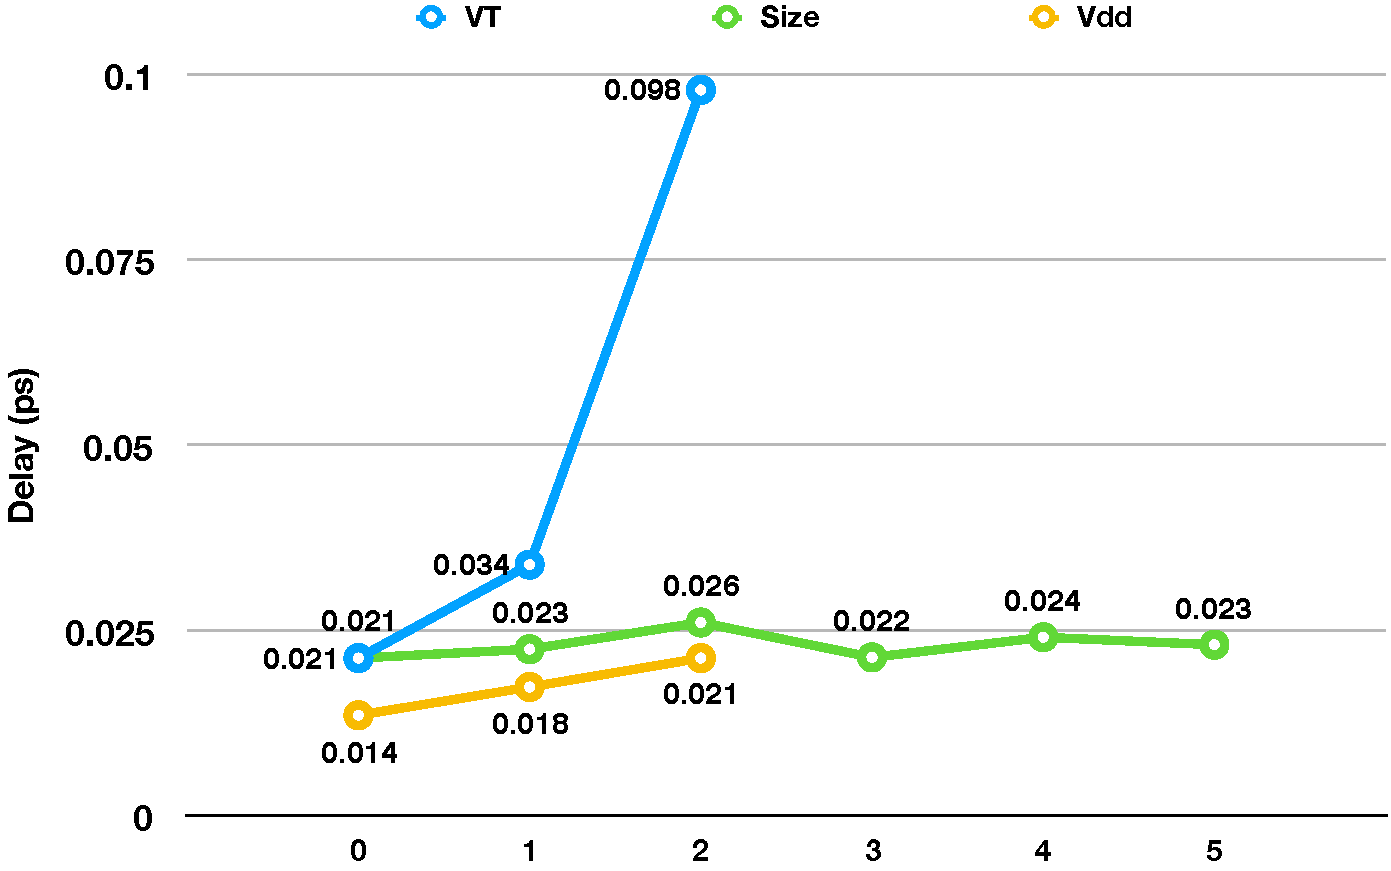
\includegraphics[width=10cm,height=5cm]{fig/delayvariation.pdf}
%   \caption{Variation of delay of an AND gate with $V_{dd}$,$V_{t}$ and $size$.}
%   \label{fig:delay1}
% \end{subfigure}%
% \begin{subfigure}{.55\textwidth}
%   \centering
%   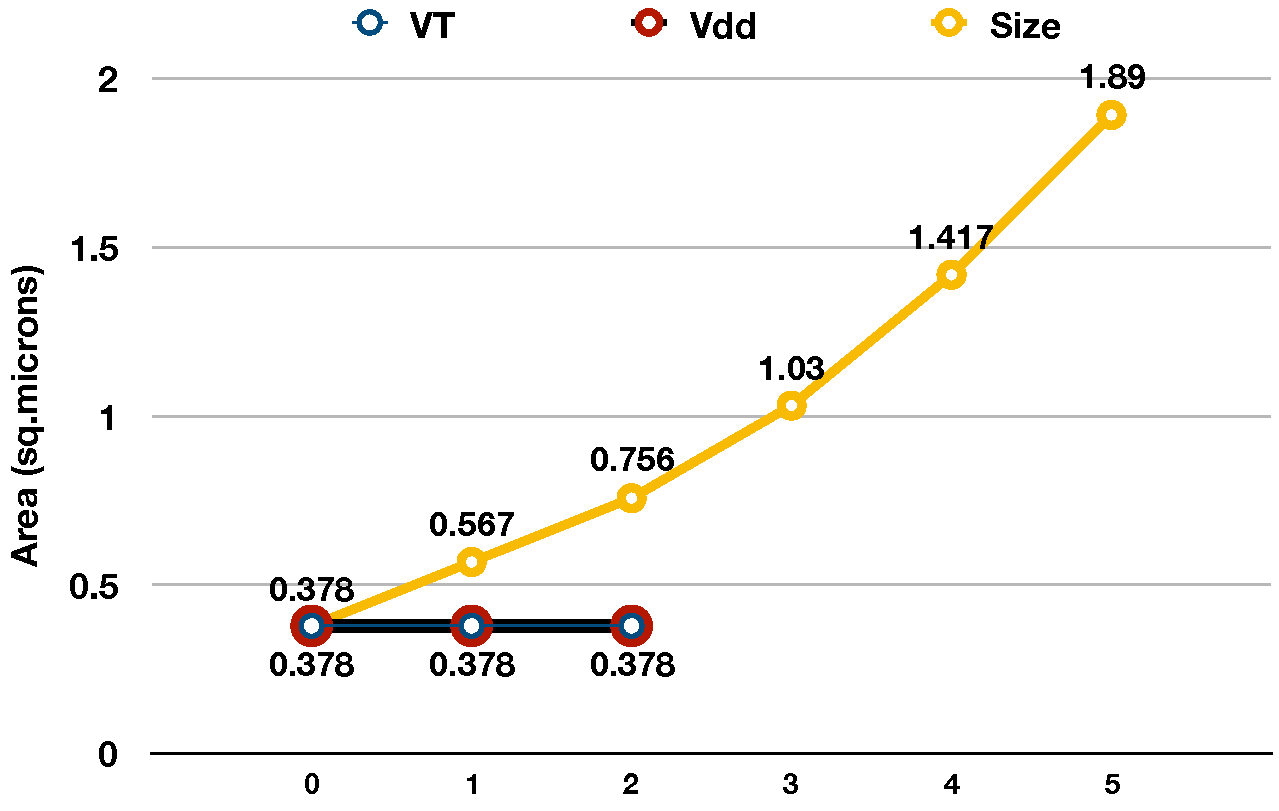
\includegraphics[width=8cm,height=5cm]{fig/areavariation.pdf}
%   \caption{Variation of area of an AND gate with $V_{dd}$, $V_{t}$ and $size$. }
%   \label{fig:delay2}
% \end{subfigure}
% \caption{Figure showing variation of delay and area of an AND with respect to $V_{dd}$, $V_{t}$ and $size$. It can be seen that delay increases with increase in $V_{dd}$, $V_{t}$ and size while area remains constant for $V_{dd}$ and $V_{t}$ scaling and increases with increase in size}
% \label{fig:delay}
% \end{figure*}


\begin{namedthm}{Observation }
Not all regions of the synthesized design contribute equally to the leakage.
\end{namedthm}
{\flushleft There} are certain areas in the design that have a higher leakage compared to other areas. In order to evaluate this, we divided the netlist into a $10 \times 10$ grid and computed the TVLA score for each region independently, thus obtaining 100 different TVLA scores corresponding to various regions in the  netlist. Figure~\ref{fig:aesopt} shows the variations in the TVLA score calculated for netlist III. 
{\sf Karna}, reconfigures the units where leakage is high, so as to reduce the overall side-channel leakage of the design without compromising the other design requirements. 


\begin{namedthm}{Observation }
The side-channel leakage from a gate depends on its  parameters.
\end{namedthm}
In order to observe the impact of each gate configuration on the side-channel leakage, we synthesized an AND-tree design with 16-bit input and 1-bit output, multiple times with different gate configurations. Each synthesis run was done with a different gate configuration. Figure~\ref{fig:gateparam} shows the TVLA scores obtained from 2000 pairs of simulated power traces for each run. It can be seen that changing 
$V_{dd}$, $V_t$ or $size$ options for a gate has an impact on the side-channel leakage of the design.

%Hence, it is important to select gate configurations that meet the design requirements but do not impact the security constraint.
%As mentioned earlier, the EDA tool optimizes the $V_{dd}$, $V_{t}$ and  size of each gate in the design in order to meet a given constraint.We now examine the impact of modifying the design choices by using an AND gate as an example. Figure~\ref{fig:power} shows the variation of dynamic power of an AND gate when the supply voltage $V_{dd}$ and threshold voltage $V_{t}$ are varied. It can be seen that increasing the supply voltage will cause the power consumed by the gate to increase by $\approx5\times-20\times$. We can also observe that the power consumed for different inputs (i.e, $00$, $01$, $10$, and $11$) is different. For example, the difference in the power consumed for inputs $11$ and $01$ at $V_{dd}=1.1V$ is $288$ pW, whereas the difference is $3.5$ pW at $V_{dd}=0.945V$. Such differences can be leveraged to distinguish between the inputs provided at the AND gate and may affect the overall security of the design. A similar observation can be made in figure~\ref{fig:sub2} for $V_{t}$ and figure~\ref{fig:sub3} for varying the gate size. 

A na\"ive approach to achieve security would be to choose gate configurations that provide highest security. However,  na\"ively choosing such gate configurations may violate other design requirements such as delay and power. 
Therefore, there is a need for a careful strategy to vary the gate parameters such that the overall security of the design improves while still meeting the desired design requirements.  
\vspace{-3pt}
% Motivation for post-placement
%It is important to note that the security countermeasures incorporated at any given stage should remain persistent throughout the other stages in the flow. For example, incorporating security at a post-synthesis stage might cause the design to violate area requirements in the placement stage thus requiring re-synthesis. Another consequence is that the tool could optimized out the proposed countermeasures thereby rendering them ineffective. 
%In this work, we therefore choose to introduce the {\sf Karna} module which selects the appropriate gate configuration for each after the design is placed. At this stage, a realistic estimation of the interconnect delay and power density is known. Thus, in this stage, we can accurately gauge the impact of the proposed security based modifications on the area, delay, and performance of the device. 

% a gate $g_{i}$ to be in the critical path of a design iff }




%The problem of securing devices against power side channel attacks has been explored since \cite{} and \cite{}. Techniques like \cite{} and \cite{} have explored software level and device level techniques to address this issue. However, software level techniques only alleviate the symptoms but fail to address the root cause of such vulnerabilities. Device level techniques rely on modifying the physical traits of the device either at gate level as in \cite{}. In this work we explore an alternative idea of mitigating power side-channels at the design level. We motivate the need for such a technique in this section. %This is what disconnected writing gets you, you idiot!

%\indent A power side-channel is said to occur when the device under test consumes drastically different power for a specific input vector than for other random inputs. Mitigating this problem would mean producing a configuration for the device such that it consumes constant or near constant amount of power for any input thereby reducing the statistical variation between the power signature for a fixed input. In device terms this would mean assigning each gate in the device a configuration such that the overall power consumption is fairly constant. 

%\indent In a typical VLSI design flow, the device typically undergoes several optimizations, each with its own objective. The primary of these requirements is performance. The recent power wall and the need for compact devices has led to the emergence of power and area as additional requirements. However, it should be noted that power and area are optimized only if the primary objective is satisfied. 

%\textbf{Observation 1: This drive for a performance optimized design cause the designers to pick gate configurations that, while making the design efficient, might make it compromise the security of the device.}

%It can be seen that while the various algorithms in the EDA flow optimize the design for one or more of performance,area or power, none of them consider the impact on the overall security of the device. This causes the algorithms to pick gate configurations that, while making the design optimal with respect to its requirements, lower the MTD of the device. 





% \indent When we observe the overall power consumption of the device, it can be divided into two components viz. static and dynamic power consumption. Static power is the power that the device consumes during the idle stage and is influenced by temperature, Threshold voltage ($V_t$) and the size of the gate ($g^i_s$). Dynamic power, is the power that is consumed when the device performs some computation, and is affected by the load capacitance ($C_i$), supply voltage $V_(dd)$, and the operating frequency ($F$). It is interesting to see the impact of modifying one or more of these device parameters on the power side-channel of the device.

% \indent Table~\ref{tab2} and~\ref{tab3} shows the leakage power and dynamic power of an inverter. It can be seen that varying $V_t$, $size$, $V_(dd)$ and load capacitance of a gate has an impact on the amount of power that the gate finally consumes. 
% \begin{table}[!ht]
% \begin{tabular}{|c|c|c|c|}
% \hline
% \textbf{Logic Level} & \textbf{$V_{(dd)_1}$} & \textbf{$V_{(dd)_2}$} & \textbf{$V_{(dd)_3}$} \\ \hline
% 00                   &               &               &               \\ \hline
% 01                   &               &               &               \\ \hline
% 10                   &               &               &               \\ \hline
% 11                   &               &               &               \\ \hline
% \end{tabular}
% \label{tab2}
% \caption{Table showing the impact of $V_(dd)$ on the power consumed.}
% \end{table}

% \begin{table}[!ht]
% \begin{tabular}{|c|c|c|c|}
% \hline
% \textbf{Logic Level} & \textbf{$V_{t_1}$} & \textbf{$V_{t_2}$} & \textbf{$V_{t_3}$} \\ \hline
% 00                   &               &               &               \\ \hline
% 01                   &               &               &               \\ \hline
% 10                   &               &               &               \\ \hline
% 11                   &               &               &               \\ \hline
% \end{tabular}
% \label{tab3}
% \caption{Table showing the impact of $V_t$ on the power consumed.}
% \end{table}
% It can be seen that varying $V_t$, $size$, $V_(dd)$ has an impact on the amount of power a gate consumes and thereby it also impacts the power side channel of the entire device. Hence there exists the need for a optimization scheme that takes into account the security of the device. In the next section we introduce Karna, a security aware power optimization scheme.




% %\indent Table~\ref{tab4} shows the various requirements that are addressed during the design manufacturing, it can be noted that security is never viewed as an objective during these stages. This is because quantifying the security or degree of "trust" in a chip is a hard problem to solve in itself. It is harder to quantify the "change" in the degree of trust due to an optimization. Figures~\ref{fig1} and ~\ref{fig2} represent two different optimization choices performed on the same design. It can be seen that 

% %\textbf{Observation 3: There exists a need to reliably quantify the impact of a design optimization on the security of the device.}

% %It can be seen that there exists a need for a design level solution that is able to quantify the impact of design optimizations on security. This will enable designers to explore security aware design optimizations such that performance goals can be achieved while minimizing the vulnerability of the device. In the next section, we will explore how existing metrics can be translated %find a better word
% %into design level requirements and a security aware power minimization scheme. 




% \section{Related Work in SMAB}
% \label{sec:related}
% \section{Related Work}
\label{sec:related}
% \todo[inline]{
% Organize related work as follows:

% Side-channel countermeasures can be applied at either the algorithm level, system level, or device level.

% Algorithm level countermeasures include masking, threshold implementations, rekeying.

% System level countermeasures include all the power noise aspects.

% Ours is most close to 
% Device level include WDDL, SABL, etc.
% }
%\subsection{Related Work:}
Side-channel attack countermeasures can be categorized as algorithmic, physical, or system-level. Algorithmic countermeasures insert additional operations that mask~\cite{akkar:2001} or split~\cite{Bilgin:2014} the sensitive computation. System-level countermeasures, such as~\cite{Wang:2013,tokunaga:2009,singh:2015,mathew:2018}, use the device's power supply to  normalize or randomize the overall power consumption. Physical countermeasures like ~\cite{Kim2017,Tiri:2004} use custom gates that consume power independent of the gate's switching. While  algorithmic and system-level countermeasures require additional circuitry, {physical countermeasures} use custom logic design methodologies to tackle the leakage. {\sf Karna} on the other hand requires no additional circuitry nor custom logic therefore has much lower overheads.  
{\sf Karna} in principle, is similar to ~\cite{Tiri:2004}, where side-channel resistant gates are realized by combining multiple standard cell gates. However, the size of each compound gate is considerably larger, resulting in a 4$\times$ increase in area. {\sf Karna} on the other hand, simply reconfigures gates in the design. Thus the area is not affected. Gate reconfigurations during the EDA flow have been used in the past to ensure low-power design~\cite{hu:12,flach:2014} and high-performance~\cite{ozdal:2012}. To the best of our knowledge, {\sf Karna} is the first to use gate reconfiguration to address side-channel leakage.

%The EDA flow is responsible for translating the design specified in a high level language like Verilog into actual hardware. Gate sizing algorithms attempt to select the best possible configuration of the gate such that the objectives at the corresponding stage are achieved. Works like~\cite{hu:12, ozdal:2012,reimann:13,li:2012,flach:2014} propose a sizing algorithm that focuses on varying the threshold voltage $V_t$ and the size of the gate in order to reduce the power consumption of the design.  While~\cite{hu:12,reimann:13} use heuristics like simulated annealing to reconfigure the gates, \cite{ozdal:2012,li:2012,flach:2014} use analytical techniques to solve the problem. However, none of the prior works attempt to leverage the EDA flow in order to counter the power side-channel. To the best of our knowledge ours is the first work try and use the gate sizing techniques to mitigate power side-channels.
%\vspace{-3pt}
\section{Conclusion and Future Work}
\label{sec:conclusion}
{\sf Karna} demonstrates that side-channel security of a device can be improved by reconfiguring the vulnerable gates in the design. This allows security constraints to be elegantly integrated into any EDA flow permitting designers to achieve design security with minimal overheads. {\sf Karna} works on a post placed netlist and is tested successfully on three popular cipher implementations and meets the desired security level (4.5) with minimal impact on area,power and delay. Our current results show drastic increase in EDA design time, mainly due to power trace collection needed for TVLA computation. In the future we plan to optimize this step by parallelization and with better side-channel metrics. Another direction of work is to evaluate {\sf Karna} to address other side-channel attacks like fault injection and timing. 


%In our proposed flow, we investigate the impact of various design optimizations on the security of the device using the metric proposed in~\cite{becker:2013}. We identify potential regions in the netlist that are vulnerable and use a gate sizing scheme to reconfigure the $V_{dd}$, $V_t$ and $size$ values in the netlist such that the overall t-score of the netlist falls under the prescribed limits. 



% \begin{itemize}
% \item \textbf{Prior Survey}: \cite{Yang2017}:Hardware Designs for Security in Ultra-Low-Power IoT Systems: An Overview and Survey; \cite{Duarte2009}: A note on the security of M ST 3; \cite{Diehl2018}: Comparing the cost of protecting selected lightweight block ciphers against differential power analysis in low-cost FPGAs; 

% \item \textbf{Attacks}: \cite{Moradi2014}:Side channel attack using static power;\cite{Alioto2010}: Leakage Power attacks; \cite{Wei2018}: I Know What You See: Power Side-Channel Attack on Convolutional Neural Network Accelerators
% \cite{Singh2017}: Improved power side channel attack resistance of a 128-bit AES engine with random fast voltage dithering.
% \item \textbf{Analysis on SideChannel Attacks}: \cite{Moos}:Static Power Side-Channel Analysis of a Threshold Implementation Prototype Chip;  \cite{Reparaz2017}: Dude, is my code constant time?; \cite{Goodwill2011}: A Testing Methodology for Side-Channel Resistance Validation;  \cite{Roy2015}:From theory to practice of private circuit: A cautionary note (This paper talks about leakage detection tests, more of an analysis than a metric, could be a section after discussing attacks); \cite{Moosa}: Glitch-Resistant Masking Revisited or Why Proofs in the Robust Probing Model are Needed; \cite{Zoni2018}: A Comprehensive Side-Channel Information Leakage Analysis of an In-Order RISC CPU Microarchitecture; \cite{Brier2004}: Correlation Power Analysis with a Leakage Model; \cite{Bache2018}: Confident Leakage Assessment -A Side-Channel Evaluation Framework based on Confidence Intervals

% \item \textbf{Metric}: \cite{Veyrat-charvillon2013}: Certify leakage of a chip; \cite{Schneider2016}:Leakage assessment methodology; \cite{Federal2017}: A Platform to Evaluate the Fault Sensitivity of Superscalar Processors; \cite{Standaert2017}: How (not) to Use Welch's T-test in Side-Channel Security Evaluations; \cite{Corre}: Micro-Architectural Power Simulator for Leakage Assessment of Cryptographic Software on ARM Cortex-M3 Processors
% \cite{Mather}: Does My Device Leak Information? An a priori Statistical Power Analysis of Leakage Detection Tests; \cite{Zhang}: Towards Sound and Optimal Leakage Detection Procedure; \cite{Reparaz}:Fast Leakage Assessment; \cite{Sadhukhan2017}: An Evaluation of Lightweight Block Ciphers for Resource-Constrained Applications: Area, Performance, and Security; \cite{Barenghi2018}: Side-channel security of superscalar CPUs Evaluating the Impact of Micro-architectural Features;

% \item \textbf{Model Using some metric to avoid attacks}: \cite{Leiserson2014}: Gate-Level Masking under a Path-Based Leakage Metric; 

% \item \textbf{Models to provide security against attacks}: \cite{DeCnudde2016}: Masking AES with $d + 1$ shares in hardware; \cite{Ghoshal2017}: Several masked implementations of the boyar-peralta AES S-Box; \cite{DeCnudde2017}: Securing the PRESENT Block Cipher Against Combined Side-Channel Analysis and Fault Attacks; \cite{Kar2018}: Reducing Power Side-Channel Information Leakage of AES Engines Using Fully Integrated Inductive Voltage Regulator; \cite{Wegener}: A First-Order SCA Resistant AES without Fresh Randomness; \cite{DeCnudde2017}: Securing the PRESENT Block Cipher Against Combined Side-Channel Analysis and Fault Attacks; \cite{Seuschek2017}: Side-channel leakage aware instruction scheduling;  \cite{Kim2017}: STBC: Side Channel Attack Tolerant Balanced Circuit with Reduced Propagation Delay; \cite{Patranabis2016}: Shuffling across rounds: A lightweight strategy to counter side-channel attacks ; \cite{Judd2016}: Proteus; \cite{Gross2018}: Generic Low-Latency Masking in Hardware;\cite{Ghoshal2018}: Lightweight and Side-channel Secure 4 × 4 S-Boxes from 
% Cellular Automata Rules; \cite{Agosta2015}:The MEET Approach: Securing Cryptographic Embedded Software Against Side Channel Attacks; 

% \item \textbf{Miscellaneous}: \cite{Levi2017}CPA Secured Data-Dependent Delay- Assignment Methodology;  \cite{Profile2014}: Optimum Leakage Recovery using Synopsys Primetime ECO Leakage Recovery Flow; \cite{Gross2018a}: Generic Low-Latency Masking in Hardware; \cite{Gierlichs2008}: Mutual Information Analysis; \cite{Peng2018}: Framework for efficient SCA resistance verification of IoT devices

% \end{itemize}



% \newpage
% \section{Summary}
% \label{chap2:conc}
% \input{Chapter2/conclusion}

%%%%%%%%%%%%%%%%%%%%%%%%%%%%%%%%%%%%%%%%%%%%%%%%%%%%%%%%%%%%




%%%%%%%%%%%%%%%%%%%%%%%%%%%%%%%%%%%%%%%%%%%%%%%%%%%%%%%%%%%%
\clearemptydoublepage
\chapter{Efficient UCB Variance: An Almost Optimal Algorithm in SMAB Setting}
\label{chap:EUCBV}
\section{Introduction}
\label{sec:introduction}

\noindent Dennard's law~\cite{dennard:74} states that the power density would remain constant with technology scaling even with the increase in MOS-device density.  With modern deep nanometer devices, optimization of power consumption has become more complex than optimization for delay or area. This is primarily due to the dominance of leakage power in the sub-100$n$$m$ technology. Techniques like supply voltage scaling and threshold voltage scaling have been used in past to reduce dynamic power consumption while maintaining/improving timing of critical path. However, in sub-100$n$$m$ regime, the exponential increase in sub-threshold leakage due to  threshold voltage scaling has caused leakage power to dominate in microprocessors~\cite{borkar:99,kim:03}. It is also to be noted that leakage power dissipation during idle state does not contribute to any useful computation. In addition, excessive leakage power dissipation can also cause power wastage leading to a  potential {\em thermal runaway}\cite{virat}. This has led to an extensive research on leakage power optimizations at different levels of the VLSI design flow under aggressive timing constraints. 

\noindent Gate-sizing and threshold voltage ($V_t$)-sizing are two efficient techniques that are employed at the design stage for reduction of leakage power under timing constraints. In particular, gate-sizing has been very effective in the early and middle stages of the physical synthesis flow.
% * <sristisravan@gmail.com> 2017-06-28T07:45:15.739Z:
% 
% Cite some papers for these statements
% 
% ^.
However, in the post-route stage, gate sizing often necessitates 
incremental placement, which can result in increase of turn-around-time of chip production~\cite{feng:09}. On the other hand, $V_t$ sizing provides enough room for significant optimization in power/timing without any effect on placement. Though, increasing the threshold voltage for a gate (say $g$) by  $V_t$ sizing can result in reducing the leakage power, it can significantly increase the delay. Hence, either gate-sizing or $V_t$ sizing or a mix of both is used to make the optimal choice of each gate depending on the design stage that the chip is present\cite{virat}.

\noindent A standard cell library consists of different versions of the same cell, one for each threshold voltage. However, the number of versions for a given cell is finite and it is limited to the discrete values of the threshold voltages specified by the foundry. Thus, it is imperative to identify cells from the standard cell library that have appropriate gate-size/$V_t$ within the set of available values to minimize the overall leakage power of the circuit without violating the timing constraints.
This optimization problem is called the {\em Timing Constrained Discrete Sizing Problem} (TC-DSP). In this paper, we focus on the TC-DSP for leakage power minimization in digital circuits. 

\noindent In addition to the sizing problem, the rapidly shrinking fabrication technology has resulted in an increase in the design optimization effort due to various factors such as multiple process, voltage and temperature corners. This in turn has resulted in an increase in the design effort (design productivity) of chips to match the estimated parameter values at the design phase to what is desirable in the  post fabrication phase. Fast convergence to high quality solutions is thereby required so as to increase design productivity and meet the consumer demand. Practically, the problem of increasing design productivity becomes important during the optimization phase of the VLSI design; as the execution time of this phase spans over hours to days. %For example, reducing optimization time for a given parameter from 2 minutes to 1 second gives more than 2 orders of magnitude speed-up. But from a practical point of view, this reduction is not valuable as the actual reduction is only 119 seconds, which is comparatively very small in the overall design time, that spans several days or months. On the other hand, reducing optimization time from 5 days to 1 hour also gives a $2 \times$ speed-up as explained in the previous case. But in this case, the actual reduction in running time is 4 days and 23 hours, which can significantly improve the design productivity. 
% * <sristisravan@gmail.com> 2017-06-28T07:43:33.360Z:
% 
% 119 seconds
% 
% ^ <slpskp@cse.iitm.ac.in> 2017-06-28T14:34:53.507Z.

\indent ITRS 2011 \cite{itrs:2011} highlights the intensity of research carried out on low power design technology improvements. However, the designers are not able to effectively leverage all the optimization choices due to runtime constraints. For example, consider a design with three cells and a standard cell library with three $V_t$ and ten gate-size choices. If we just consider $V_t$ scaling for power optimization, the search space is $3^3$. Further, if the designer uses gate-sizing, the search space increases to $3^{10}$. Finally, if a mixed sizing technique is employed, the search space increases to $3^{30}$. Thus we can see that, design productivity heavily suffers due to a large exploration space available at each phase of optimization. The authors in  \cite{kahngtalk} list the following three hypothetical steps to improve design productivity without compromising power goals namely:  \begin{itemize}
    \item  \textbf{Optimized back-end:} mixed height library floorplan/placement, ultimate place/route, power/clock distribution;
    \item  \textbf{Modeling/sign-off criteria:} tightened Back End Of Line (BEOL) corners, reduced guardband and Adaptive Voltage Scaling (AVS) aware sign-off; and,
    \item  \textbf{Bespoke,design-specific-flow:} predictive one-pass flow, optimal tool usage.
 \end{itemize} 
 Consider the following pseudocode which represents the template for any iterative greedy gate-sizing optimization algorithm as seen in \cite{hu:12},\cite{hu:13},\cite{mok:12}, and \cite{reiman:13}. The algorithm takes as inputs: the Netlist $C$; containing $N$ gates, that needs to be optimized, a multi-$V_t$ standard cell library, the target frequency $F$ and a function $\alpha(C)$. The function $\alpha(C)$ takes as inputs the circuit C, the timing values for each logic element got by performing a Static Timing Analysis (STA), and other foundry specific parameters for the different logic elements in C, to compute a cost for every gate in C.
\begin{algorithm}
%\algsetup{linenosize=\tiny}
\scriptsize
\LinesNumbered
\title{Greedy Leakage optimization algorithm}
\caption{The template for an iterative greedy leakage optimization algorithm }
\label{alg:naive}
    \KwIn{1) Netlist of the given circuit $C$ containing $N$ gates represented as a Directed Acyclic Graph (DAG). 2) Target frequency $F$. 3) A multi-$V_t$ standard cell library containing multiple cells with different threshold voltages and sizes for every gate; and, 4) Cost function $\alpha(C)$ that computes a cost for every gate in $C$.}
    \KwOut{A leakage optimized netlist running at the target frequency $F$.}
 $N \leftarrow gate\ count$\; 

    \textit{Initial Configuration:} Assign to each of the $N$ gates a cell from the standard cell library matching its functionality. The $V_t$ and $size$ of each gate shall vary with different methods employing this template\;
Set iteration count to $1$\;
    Run Static Timing Analysis (STA) and compute $\alpha(C)$\; 
    A $\leftarrow$ list of gates sorted in decreasing order according to cost computed by $\alpha(C)$\;
   
    \While{A not empty } {
        \textit{Gate replacement:} Consider the first element of A (the gate g with the largest cost) and replace it with its unexplored slower choices (increase $V_t$ or decrease the $size$) so as to reduce the leakage power. Mark the choice as explored for gate g\;
        Estimate the new power and the new delay of the circuit $C$ by performing STA\;
        \If{delay violated} { 
        \textit{Backtrack procedure:} 
            Undo the gate replacement and delete it from A\;
        }
        \Else {
            Increment iteration count\;
            Compute $\alpha(C)$\;
	    If all the choices for gate g, available in the standard cell library, have been explored delete it from A\;
        }
        Sort the gates in A according to decreasing order of cost computed by $\alpha(C)$\;
    }
\end{algorithm}

\noindent It can be observed that the convergence of the above algorithm crucially depends on the initial configuration, the cost function $\alpha(C)$ which is used to determine the candidate gate for replacement and the number of STA calls.  Our proposed leakage optimization technique (\textit{MLTimer}) aims at resolving these bottlenecks. The main contributions of this work are as follows:
\begin{itemize} %check if ieee uses itemize or enumerate??
\item It has been empirically observed that there exists significant correlation between the timing slacks of gates in the current iteration to the gate replacements in the successive iterations. The outcome of this replacement is the fast convergence of the leakage optimization algorithm in lesser number of iterations;
     \item  It can also be seen that a smart one-pass tool that can leverage the right optimization technique at the appropriate stage of the flow can improve design productivity significantly. A novel Support Vector Machine (SVM) based classifier, which provides a good initial design configuration is used to generate a leakage optimal design at the end;
     \item The \textit{MLTimer} algorithm, which leverages the high iterative correlation between timing slacks in the current iteration and the gate replacements in the successive iterations, thereby enabling  {\em lazy timing analysis} to significantly improve the runtime; and, 
\item An {\em Adaptive Window sizing (AWS) scheme for decision making} to perform {\em multiple  replacements} between successive timing updates.

%\item A lazy adaptive heuristic,  that uses the solution provided by the learning algorithm to provide a leakage optimized solution while meeting the delay constraints.
%\item To the best of our knowledge, this is the first work to use learning to solve the leakage optimization problem.
%\item The solutions produced by our algorithm {\em Learntimer} are at least {\em an order of magnitude} faster while retaining the same solution quality as that of iterative greedy heuristics.
%\item We demonstrate the efficiency of our algorithm on the ISPD2012 benchmarks.
\end{itemize}
To the best of our knowledge, this is the first work that employs ML technique to solve the well known leakage optimization problem. We demonstrate the efficiency of our algorithm on both the ISPD2012 benchmarks and a homegrown RISC-V (SHAKTIC) processor that runs linux~\cite{riscv}. 


% \begin{figure*}[!ht]
%  \begin{center}
%  \includegraphics[scale=0.45]{fig/predict}
% \captionsetup{singlelinecheck=off}
% \caption [The figure shows the impact of the three hypothetical design steps on solution quality and design time. The proposed steps are Optimized back-end: $(mixed height library floorplan/placement, ultimate place/route, power/clock distribution)$ Modeling/sign-off criteria $(tightened BEOL corners, reduced guardband and AVS aware sign-off)$.\#1: Bespoke,design-specific-flow $(predictive one-pass flow, optimal tool usage)$ ]{The figure shows the impact of the three hypothetical design steps on solution quality (QoR) and design time. The proposed steps are 

%  \label{fig:kahng}
%  \end{center}
% \end{figure*}
 
The rest of the manuscript is organized as follows: Section~\ref{sec:background}  presents the problem along with the literature survey. Section \ref{sec:motivation} describes the need for a learning based leakage optimization technique. Section~\ref{sec:proposed} describes our proposed algorithm while the experimental setup is highlighted in Section~\ref{sec:experiment}. The results are presented in ~\ref{sec:results}. Section~\ref{sec:conclusion} concludes the paper.
% * <sristisravan@gmail.com> 2017-06-28T07:46:32.613Z:
% 
% What does STA mean?
% 
% ^.


In this chapter, we look at a novel variant of the UCB algorithm (referred to as Efficient-UCB-Variance (EUCBV)) for minimizing cumulative regret in the stochastic multi-armed bandit (SMAB) setting. EUCBV incorporates the arm elimination strategy proposed in UCB-Improved \citep{auer2010ucb} while taking into account the variance estimates to compute the arms' confidence bounds, similar to UCBV \citep{audibert2009exploration}. Through a theoretical analysis we establish that EUCBV incurs a \emph{gap-dependent} regret bound of {$O\left( \dfrac{K\sigma^2_{\max} \log (T\Delta^2 /K)}{\Delta}\right)$} after $T$ trials, where $\Delta$ is the minimal gap between optimal and sub-optimal arms; the above bound is an improvement over that of existing state-of-the-art UCB algorithms (such as UCB1, UCB-Improved, UCBV,  MOSS). Further, EUCBV incurs a \emph{gap-independent} regret bound of {$O\left(\sqrt{KT}\right)$}  which is an improvement over that of UCB1, UCBV and UCB-Improved, while being comparable with that of MOSS and OCUCB. Through an extensive numerical study, we show that EUCBV significantly outperforms the popular UCB variants (like MOSS, OCUCB, etc.) as well as Thompson sampling and Bayes-UCB algorithms. 

    The rest of the chapter is organized as follows. We elaborate our contributions in Section~\ref{sec:contri} and in Section~\ref{sec:eucbv} we present the  EUCBV algorithm. Our main theoretical results are stated in Section~\ref{sec:results}, while the proofs are established in Section~\ref{sec:proofTheorem}. Section~\ref{sec:expt} contains results and discussions from our numerical experiments and finally we summarize in Section \ref{sec:conc}.
    %and Appendix \ref{sec:app:EUCBV} contains the proofs of the lemmas that have been used for proving the main result.
    
%scriptsize
\section{Background on Discrete Sizing Problem}
\label{sec:background}
The TC-DSP problem has been studied extensively in the last 30 years and various optimization techniques have been proposed. In this section, we present a summary of the these efforts.



\subsection{The TC-DSP Problem}
%should check if this wording reflects the equation based formulation.

\noindent Consider a circuit $C$ containing $N$ gates. Let each of the gate be realizable using $m$ choices made available in the standard cell library provided by the standard cell library. Starting from the primary input(s), we define the instant that a signal reaches an input of a gate $g_i$ as the arrival time $A(i)$. Similarly, starting from the primary output(s), we define the maximum limit imposed for each arrival time to ensure operation of the  circuit at the target frequency as the required arrival time $R_{a}(i)$. Slack at the gate $g_i$ is defined as $R_{a}(i) - A(i)$. A positive slack implies that the timing constraint is satisfied, and a negative slack implies that the timing constraint at the particular gate is violated \cite{taucontest}.\\




%Let each of the gate $g_i$ be realizable using several choices of $V_t$ made available in the foundry provided standard-cell library.
 Let $x_{i}^{j}$ denote a discrete variable defined as follows:\\
  \begin{equation}
   {x_{i}^{j}} =
   \left\{
           \begin{array}{lllll}
                  1, \ {\bf if}\ i^{th} gate\  in\ the\ given\ circuit\ is\ realized\\
                  \  \  \ \ with\ j^{th}\ choice\ \ in\ the\ standard\\
                  \   \  \ \ cell\  library\\
                  0, \ {\bf otherwise}\\
          \end{array}
  \right.
  \end{equation}
 
 
 
%
\noindent The optimization problem is to find $x_{i}^{j}$ for lowest leakage power, without violating the critical path timing. Let $fanin(i)$ be the set of all gates driving the $i^{th}$ gate in the circuit. Let $p_{i}^{j}$ and $d_{i}^{j}$ be the power and delay of the gate $g_{i}$ when realized with the $j^{th}$ choice in the standard cell library. $PO(C)$ and $PI(C)$ denote the set of  primary outputs and  primary inputs respectively of the given circuit $C$; and, $T$ denote the timing budget assigned to $C$. The leakage minimization problem for C can be formally stated as follows:
\begin{equation}\label{opt_eqn_1} {\Large{\underset{}{\operatorname{minimize}}\sum_{i=1}^{N} \sum_{j=1}^{m} x_{i}^{j} p_{i}^{j}}}  \end{equation}
\indent \indent \indent \indent \indent such that
\begin{equation}\label{opt_eqn_2} \sum_{j=1}^{m} x_{i}^{j} = 1, \forall i, 1 \leq i \leq N\end{equation}
%\begin{equation}\label{opt_eqn_3}  x_{g_{i,j}} \in \{0,1\}, \forall i, 1 \leq i \leq N_{gate}; \forall j, 1 \leq j \leq m \end{equation}
    \begin{equation}\label{opt_eqn_4} A(i) + \sum_{j=1}^{m} d_{i}^{j} x_{i}^{j} \le A(k), \forall k \in fanin(i)\end{equation}
\begin{equation}\label{opt_eqn_5} A(O) \le T, \forall O \in PO(C) \end{equation}
\begin{equation}\label{opt_eqn_6} A(I) \ge 0, \forall I \in PI(C)\end{equation}\\
\begin{equation} \label{opt_eqn_7} slew(x_{i}^{j}) < max slew(x_{i}^{j}), \forall i,1 \leq i \leq N  \end{equation}
\begin{equation} \label{opt_eqn_8} capacitance(x_{i}^{j})<max capacitance(x_{i}^{j}),  \forall i,1 \leq i \leq N \end{equation} \\

\noindent In the above equations~\ref{opt_eqn_5} and \ref{opt_eqn_6}, $A(O)$ and $A(I)$ denote the arrival-times at primary output wires and primary input wires of $C$ respectively. Equation~\ref{opt_eqn_1} presents the objective function that minimizes the leakage power of the given circuit.
Equation~\ref{opt_eqn_2} ensures that exactly one version of gate $i$ is used among its available $m$ choices.
Equations~\ref{opt_eqn_4}, \ref{opt_eqn_5} and \ref{opt_eqn_6} ensure that the arrival-time constraints are met for all the gates, primary inputs and primary outputs of $C$ respectively.

\noindent The delay of a gate is obtained by using the input slew and load capacitance values to index to an array in the standard cell library. The replacement of a gate with its higher $V_t$ or lower $size$ variants might violate the slew constraints in its fanout cone or capacitance constraints in its fanin cone. Equations ~\ref{opt_eqn_7} and~\ref{opt_eqn_8} ensure that the replacement does not cause such violations.
This formulation has been studied extensively in \cite{hu:12}, \cite{hu:13},\cite{reiman:13}, \cite{li:12}, \cite{ozdal:12},\cite{hu:13}, and \cite{rahman:12} .

\subsection{Prior Work}

Though, the above presented TC-DSP problem formulation has been studied extensively in the last 30 years, the works could not be compared as there was no standard framework to evaluate each proposed solution. Another challenge was that the solutions were largely academic and could not be extended to meet modern technologies. The various challenges faced during the circuit optimization phase in an industrial flow were formulated in \cite{ozdal:12}. The ISPD 2012\cite{ispd:12} contest framework was setup to address the above two challenges. 
It had 7 benchmark netlists. The netlist sizes ranged from $25,000$ gates to $9,50,000$ gates. Each netlist has i) a Verilog file representing the functionality of the circuit; ii) a SPEF file that had the capacitance and resistance value for each net in the design; and, iii) two delay constraint files which could be used to realize a fast and a slow version of the same design respectively.

The various solutions used to tackle the discrete sizing problem can be broadly classified as, i) Non analytical methods which use heuristic based techniques to solve the problem and ii) Analytical methods which try to solve it by posing the problem as a Lagrangian relaxation or as a Convex Optimization problem.

\begin{itemize}
\item \textbf{Non-Analytical Methods:}  Non-Analytical methods rely on greedy heuristics as shown in\cite{hu:12},\cite{mok:12},\cite{reiman:13} and  %dp formulation,
\cite{rahman:12}. %rahman and sachen
        A sensitivity guided heuristic to solve the TC-DSP was proposed by \cite{hu:12}. The authors use a \textit{go-with-the winners} approach. They also observe that evaluating the benchmarks using varying cost functions yields better results. Their proposed solution outperforms the winners of the ISPD2012 contest by a significant margin. A comprehensive survey of the existing leakage optimization techniques is presented in \cite{mok:12}. The authors in \cite{mok:12} also propose a peephole optimization based technique for gate sizing. A simulated annealing based approach to solve the TC-DSP was presented in \cite{reiman:13}. They use the \textit{fanout-of-4 rule} and \textit{logic effort} to initialize the netlist to a good initial configuration. However, their solution fails to achieve timing closure on all benchmark circuits. A $V_t$ optimization technique, that uses a new cost function  $\frac{\delta slack}{\delta leakage}$ where $ \delta slack$, $\delta leakage$ represent the slack variation and leakage variation due to the change in the $V_t$ of the cell respectively, is employed in \cite{rahman:12}. The gates are ranked in ascending order based on the above metric and swapped if there is no timing violation. 
        Dynamic programming based solutions were proposed by \cite{li:12}, \cite{Ketkar:09},\cite{Liu:09} while works like \cite{livramento:14}, \cite{ren:08} employed a network flow based solution. %\cite{Liu:09} use GPU to speedup their DP based solution.
% find the two references.


\item \textbf{Analytical Methods:} Analytical methods try to solve the problem by posing it as 
Convex Optimization Formulation or Lagrangian Formulation. Of these two, the Lagrangian relaxation problem has been shown to be more effective as seen in \cite{ozdal:12}, \cite{li:12},\cite{livramento:14},\cite{flach:13},\cite{livramento:13} and \cite{sharma:15}. The objective is to minimize the total leakage power in the circuit while penalizing any delay violations. A modified formulation that takes into account the capacitance and slew conditions is presented in \cite{li:12}. Their LR formulation improves both the solution quality and the runtime significantly. A multi-threaded approach to solve the problem is presented in \cite{sharma:15}. A new metric to identify the candidate gates that could be replaced with different $V_t$/$size$ choices is presented in \cite{reis:16}. 

\end{itemize}

Initial STA engines always processed an entire design, which is impractically expensive for evaluating every 
        replacement~\cite{papa:10}. It is to be noted that replacing the $V_t$/$size$ of a gate $g_i$, changes the arrival times of gates only in the fan-in and fan-out cones\footnote{Fan-in/Fan-out cone of a gate $g$ is defined as the sub-circuit that drives/is driven by the gate $g$\cite{abramovci}.} of $g_i$, while the arrival times of other gates remain unaffected. By performing STA for the entire design, we may end up computing known values repeatedly. 
        To improve the efficiency of the STA engine, several {\em incremental} STA techniques have been proposed in the past~\cite{lee:95},\cite{abato:96},\cite{sapatnekar:96},\cite{mondal:04},\cite{das:06}. In~\cite{lee:95}, {\em incremental} STA is performed by solving the {\em incremental longest path problem}, with a novel algorithm which is linear in the number of edges in the {\em dominance fan-out cone}. In~\cite{abato:96}, a frontier is established by recording the leftmost and rightmost gates in the fan-in and fan-out cone of each gate that gets affected by the change in relative timing values.
Based on a request, incremental timing analysis is performed on the modified design
employing the recorded frontiers of change to limit the timing analysis to 
the {\em affected} regions of the circuit alone. An input based path sensitization approach 
was used for incremental STA in~\cite{sapatnekar:96}.
On a similar note, in~\cite{coudert:97}, the incremental timer is accelerated by only updating a 
set of gates that are in the neighbourhood of the gate whose timing value has been updated. 
In~\cite{mondal:04}, timing queries were modeled using temporal logic and an efficient 
algorithm was proposed to answer those queries. Similarly, in~\cite{das:06}, a more 
efficient incremental STA algorithm which exploits the circuit structure was proposed. 
In all these works, path based algorithms were proposed to 
increase the performance of incremental STA, but none of them except~\cite{abato:96} looked 
at reducing the number of times the incremental STA needs to be performed. 
Even in~\cite{abato:96}, although incremental STA is not performed in every iteration, 
nonetheless some computation is performed in every iteration relating to the signal propagation. 
As a result, the running time complexity does not decrease significantly compared to the use of a normal STA. 
E.g., in~\cite{hu:12}, in spite of using a state-of-art incremental timer, the optimization 
        took greater than $20$ hours for the larger benchmarks $(\ge 540,000)$ in the ISPD 2012 suite. It can be seen from the above works that the STA engines reported so far consume a significant time. The number of times the STA needs to be performed (timing updates) grows linearly with the size of the circuit. Reducing the number of times such updates are performed results in a reduction in the overall running time of the algorithm. This reduction without compromising on the solution quality is the challenge that forms one of the central themes of this paper.



\noindent In the last four years, Machine Learning techniques have shown promise in solving complex optimization problems across various domains \cite{prowatch}. Learning based techniques have also been used to optimize specific bottlenecks in VLSI-CAD as shown in \cite{kahng:2} and \cite{kahng:3}. However to the best of our knowledge ours is the first work to employ Machine Learning for the problem of gate sizing.

%compare both non-analytical and analytical methods.

%~\cite{hu:12}, 



%The TC-DSP is presented as an instance of Lagrangian Relaxation (LR) problem in~\cite{Hu:11}. The objective is to minimize leakage and the algorithm places a penalty for any delay violations. The timing constraints are introduced in the LR formulation.  The netlist is modeled as a directed acyclic graph and the discrete gate version characteristics are based
%on timing tables provided by the gate library. A Dynamic Programming algorithm
%based on critical tree extraction is proposed to solve the LR optimization problem for discrete gates. An accurate timer is used for sign-off and slack computation.

%ideas that this section should contain: why do we need to take this approach.
%
%
%





\section{Motivation}
\label{sec:motivation}
 The ISPD gate-sizing contests aimed at producing robust solutions that could be easily integrated with an industrial flow. However, as pointed out in \cite{reis:16}, \cite{kahng:16} and \cite{kahng:14}, there still exists some significant challenges. As shown in \cite{kahng:14}, while the proposed solutions worked well in the framework of the contest, optimality was not guaranteed when technology nodes were changed. In this section we present an overview of the common bottlenecks that affect the robustness of the current solutions thus highlighting the need for the proposed \textit{MLTimer} solution. Our observations are as follows: 
\begin{itemize}
    \item \textbf{Initial configuration (line 2 of Algorithm~\ref{alg:naive})}: The algorithm needs to initially choose for every gate in their circuit, a cell of similar functionality from the multiple available cells specified in the standard cell library (typically three $V_t$ and ten $size$ options). Some of the recently proposed optimization techniques such as \cite{ozdal:12}, \cite{hu:12},\cite{li:12},\cite{flach:13}, and \cite{livramento:13} initialize all the gates in the netlist with a low power configuration using the largest $V_t$ and smallest $size$. However in an industrial flow this might not be possible as power optimization might be performed several times during each stage of the design flow. Initializing to a power optimal configuration  might create additional problems during the placement and routing stages as the final solution, while meeting the power constraints, might cause violations in the placement and routing constraints.    
  
    \item \textbf{Cost Function $\alpha(C)$}: Heuristic based solutions rely on cost functions to identify the candidate gate for optimization as seen in line 7 of Algorithm~\ref{alg:naive}.  However as seen in \cite{hu:12}, a single cost function for all designs might not be the best option. A poorly chosen cost function can lead to a sub-optimal solution and can increase the overall runtime of the algorithm. %elaborate talk about the impact of the cost function and 
    \item \textbf{Number of Static Timing Analysis (STA) calls (line $8$ of Algorithm~\ref{alg:naive})}: It can be seen from line $8$ of algorithm~\ref{alg:naive} that each replacement  necessitates an STA call to check whether the replacement has caused any timing violations. The number of STA calls made during the iterative process largely contributes to the overall runtime overheads. 

\end{itemize}

\noindent Thus, it is important to note that the quality of any leakage optimization heuristic is affected by the initial configuration, cost function and number of STA calls. We present a few empirical observations and inferences that can be leveraged to improve the above three factors.

\noindent {\bf Observation I}

\noindent Initializing each gate in the netlist  with random choices of both $size$ and $V_t$ (heterogeneous configuration) yielded better solutions in terms of  leakage power, delay and run time than the traditional approach. This is because, as we move to lower nanometer technologies, the delay and power do not scale linearly with $size$ and $V_{t}$. As a result, using a sub-optimal initial configuration might necessitate additional optimizations such as delay recovery, fixing slew and capacitance violations thereby resulting in a large running time. However the problem of finding the right initial configuration and the right cost function is impractical as it requires solving the entire TC-DSP in the initial stage. However as shown in Table~\ref{Tab:tab1}  several circuits can be seen to share \textit{structurally similar} sub-circuit patterns. Two sub-circuits are said to be \textit{structurally similar} if there exists an isomorphism (one-to-one mapping of vertices and edges) between them.  We leverage this observation to find the best possible initial configuration for one instance of the sub-circuit and  reuse the same for other occurrences of the sub-circuit. This has resulted in an initial configuration that causes significant reduction in both the overall execution time and the leakage power.
%A gate that has high negative slack could be subjected to delay optimization ($V_t$ downscaling or upsizing) whereas a gate with high positive slack could be subjected to power optimization. Hence, we need to identify the right operating conditions that affect the final configuration of the gate.

%if possible insert table to support the first point.

%\indent Consider the following example ~\ref{fig:example1}. Gate $G_1$ has same fanin and fanout gates but gets assigned different $V_t$ and $gate-size$ configurations. This is because the $G_1$ in ~\ref{fig:example1} has different slack than $G_1$ in ~\ref{fig:example2}. \textbf{It is not enough if the circuits share the same subcircuit pattern, they should also be under identical design conditions.}. This is illustrated in ~\ref{fig:example3} and ~\ref{fig:example4} where the same gate gets assigned same $V_t$ and $gate size$ even though they dont share a completely identical subcircuit pattern but because they share identical operating conditions.

%\indent From the examples and ~\ref{Tab:tab1} we see that different designs have several similarities which could be leveraged to predict a good initial configuration. While we might not be able to predict the exact final solution, the predicted solution can be used as a starting point for optimization. 



\begin{table*}[!t]
\centering
    \caption{Table showing the number of shared patterns across benchmarks. Each pattern is formed by using the gate along with its fanins and fanouts. The values highlighted in bold represent the total number of possible patterns for that particular benchmark. Element i,j represents the number of overlapping patterns of benchmark i in benchmark j.}
    \label{Tab:tab1}

    \begin{tabular}{ |p{2.2cm}| p{1cm}| p{1.2cm}| p{1.7cm} |p{1.4cm} | p{1.2cm}|p{1.4cm}|p{1.4cm}|p{1.4cm}|}
\hline
        \textbf{ Benchmark} & \texttt{DMA} & \texttt{pci} &\texttt{des\_perf} &\texttt{vga\_lcd} &\texttt{b19} &\texttt{leon3mp} &\texttt{netcard} & \texttt{ShaktiC} \\ \hline
    \texttt{DMA}       & \textbf{23,109} & 19,663          & 20,558           & 15,439           & 21,899           & 17,703           & 18,225           & 20,330           \\ \hline
\texttt{pci}       & 14,898          & \textbf{29,844} & 29,015           & 28,845           & 29,284           & 26,426           & 26,463           & 22,316           \\ \hline
\texttt{des\_perf} & 90,475          & 86,729          & \textbf{102,427} & 83,768           & 96,677           & 56,599           & 56,535           & 72,306           \\ \hline
\texttt{vga\_lcd}  & 15,439          & 25,316          & 27,339           & \textbf{147,812} & 41,068           & 69,696           & 58,099           & 100,034          \\ \hline
\texttt{b19}       & 182,984         & 166,217         & 181,228          & 166,372          & \textbf{212,674} & 141,619          & 139,733          & 156,877          \\ \hline
\texttt{leon3mp}   & 470,252         & 460,774         & 484,694          & 436,798          & 467,000          & \textbf{540,352} & 538,939          & 495,941          \\ \hline
\texttt{netcard}   & 813,634         & 809,793         & 834,303          & 785,423          & 796,790          & 860,397          & \textbf{860,949} & 777,582          \\ \hline
\texttt{ShaktiC}   & 120,422         & 86,762          & 72,306           & 100,034          & 134,521          & 94,361           & 115,425          & \textbf{174,756} \\ \hline
 \end{tabular}
    
\centering

\end{table*}



\begin{table*}[!t]
\centering
    \caption{Table showing the relative number of shared patterns across benchmarks. Each pattern is formed by using the gate along with its fanins and fanouts. The values highlighted in bold represent the total number of possible patterns for that particular benchmark.  Element i,j represents the percentage of overlapping patterns of benchmark i in benchmark j.}
    \label{Tab:tab13}

    \begin{tabular}{ |p{2.2cm}| p{1cm}| p{1.2cm}| p{1.7cm} |p{1.4cm} | p{1.2cm}|p{1.4cm}|p{1.4cm}|p{1.4cm}|}
\hline
        \textbf{ Benchmark} & \texttt{DMA} & \texttt{pci} &\texttt{des\_perf} &\texttt{vga\_lcd} &\texttt{b19} &\texttt{leon3mp} &\texttt{netcard} & \texttt{ShaktiC} \\ \hline
   \texttt{DMA}       & 100 & 85  & 89  & 67  & 95  & 77  & 79  & 88  \\ \hline
\texttt{pci}       & 50  & 100 & 97  & 97  & 98  & 89  & 89  & 75  \\ \hline
\texttt{des\_perf} & 88  & 85  & 100 & 82  & 94  & 55  & 55  & 71  \\ \hline
\texttt{vga\_lcd}  & 10  & 17  & 19  & 100 & 28  & 47  & 39  & 68  \\ \hline
\texttt{b19}       & 86  & 78  & 85  & 78  & 100 & 67  & 66  & 74  \\ \hline
\texttt{leon3mp}   & 87  & 85  & 90  & 81  & 86  & 100 & 100 & 92  \\ \hline
\texttt{netcard}   & 95  & 94  & 97  & 91  & 93  & 100 & 100 & 90  \\ \hline
\texttt{ShaktiC}   & 69  & 50  & 41  & 57  & 77  & 54  & 66  & 100 \\ \hline 
 \end{tabular}
    
\centering

\end{table*}


% \begin{figure} [!h]
% \begin{circuitikz} \draw %[scale=0.5\textwidth]
% %\begin{minipage}{0.5\textwidth}
% (0,2) node[and port] (myand1) {\footnotesize$G_1$ ($SV_t$)}
% (0,0) node[and port] (myand2) {$G_2$($SV_t$)}
% (2,1) node[or port] (myor) {$G_3$($SV_t$)}
% (4,2) node[and port] (myand3){$G_4$($SV_t$)}
% (4,0) node [and port] (myand4){$G_5$($SV_t$)}
% (myand1.out) -- (myor.in 1)
% (myand2.out) -- (myor.in 2)
% (myor.out)--(myand3.in 1)
% (myor.out)--(myand4.in 1);

% \end{circuitikz}
% \qquad
% \begin{circuitikz} \draw %[scale=0.5\textwidth]
% (0,2) node[and port] (myand1) {$G_1$}
% (0,0) node[and port] (myand2) {$G_2$}
% (2,1) node[or port] (myor) {$G_3$}
% (4,2) node[and port] (myand3){$G_4$}
% (4,0) node [and port] (myand4){$G_5$}
% (myand1.out) -- (myor.in 1)
% (myand2.out) -- (myor.in 2)
% (myor.out)--(myand3.in 1)
% (myor.out)--(myand4.in 1);
% %\end{minipage}
% \end{circuitikz}
% \caption{Consider Gate $G_1$ in both the circuits. $G_1$ has the same fanin and fanout gates but gets assigned different $V_t$ and $gate size$}
% \label{fig:example1}

% \end{figure}






% \begin{circuitikz} \draw
% (0,2) node[and port] (myand1) {}
% (0,0) node[and port] (myand2) {}
% (2,1) node[xnor port] (myxnor) {}
% (myand1.out) -- (myxnor.in 1)
% (myand2.out) -- (myxnor.in 2);
% \end{circuitikz}
% \caption{Consider Gate $G_1$ in both the circuits. $G_1$ has the same fanin and fanout gates but gets assigned different $V_t$ and $gate size$}
% \label{fig:example3}

% \begin{circuitikz} \draw
% (0,2) node[and port] (myand1) {}
% (0,0) node[and port] (myand2) {}
% (2,1) node[xnor port] (myxnor) {}
% (myand1.out) -- (myxnor.in 1)
% (myand2.out) -- (myxnor.in 2);
% \end{circuitikz}
% \caption{Consider Gate $G_1$ in both the circuits. $G_1$ has the same fanin and fanout gates but gets assigned different $V_t$ and $gate size$}
% \label{fig:example4}

\noindent {\bf Observation II:}

\noindent A traditional greedy heuristic for the TC-DSP involves the following two stage validation process for every replacement,
\begin{itemize}
\item {\it Local validation stage:} In this stage a gate ($g$) with the highest slack is assigned the next slower version ($V_t$ upscaled or $size$ reduced) to reduce the leakage power, without violating the timing constraint of $g$.
\item {\it Global validation stage:} The assignment of the entire circuit is validated by performing an incremental STA  and the arrival times/slacks are updated for all gates\footnote{Usually arrival times are associated with a net. 
In this paper, we represent the arrival time of a gate as the arrival time at the output of the gate}.
\end{itemize} 

\noindent It is interesting to note that in a slack-based greedy heuristic algorithm as described in~\cite{mok:12}, the gates that are higher in the ordering in the current iteration are successively replaced {\it with a high probability} in the next few iterations. We call this correlation between iterations as {\it iterative correlation}. Applying the greedy heuristic on the \texttt{c432} benchmark circuit from the ISCAS benchmark suite, where the gates were ordered in the decreasing order of slack at the end of each iteration, we see that the gates $51, 59, 70$ and $67$ that were in the top $5$ before iteration $1$, got replaced in successive iterations in the same order as given below. Here $\pi_i$ denotes the ordering of gates at the end of iteration $i$. The integers in the lists below denote the gate IDs. The gates that are {\it underlined} are the ones which get replaced in the respective iterations. It was also observed that the algorithms spend a majority of their running time in the global validation stage.\footnote{It can be noted that Gate $51$ is at the top of the list for both $\pi_1$ and $\pi_2$, as it had large amount of positive slack even after replacement in iteration $1$ and that the standard cell library used has more than two $V_t$ versions.} 
\vspace{0.1cm}
% * <sristisravan@gmail.com> 2017-06-28T07:47:57.575Z:
% 
% explain a bit on c432 and b14, maybe in footnote.. i didn't understand this terminology
% 
% ^.
\\
\noindent $\pi_1$: $\underline{51}$  $52$  $59$ $70$ $67$ $72$ $71$ $58$ $74$ $65$ $56$\ldots\\
$\pi_2$: $\underline{51}$ $52$ $59$ $70$ $67$ $72$ $71$ $58$ $74$ $65$ $56$\ldots\\
$\pi_3$: $\underline{59}$ $70$ $67$ $72$ $71$ $58$ $74$ $65$ $56$ $52$ \ldots\\
$\pi_4$: $\underline{70}$ $67$ $59$ $72$ $71$ $58$ $74$ $65$ $56$ $52$\ldots\\
$\pi_5$: $\underline{67}$ $59$ $72$ $71$ $58$ $70$ $74$ $65$ $56$ $52$\ldots

\vspace{0.1cm}

\noindent \noindent{\textbf{ Inference}}: One of the inferences from the above observation is that there exists a scope for reducing the run-time of the algorithm by exploiting the iterative correlation to postpone the global validation. In other words, the STA can be performed  after {\it multiple} gate replacements ({\it lazy timing evaluation}) in contrast to performing the same after every single gate replacement. This in turn,  significantly reduces the number of STA runs and thereby, the running time of the entire algorithm. To empirically justify the above inference, the following experiment was conducted. The greedy heuristics in~\cite{mok:12} was employed on the \texttt{c432} circuit with one gate being replaced in each iteration. We define $\pi^{'}_i = (gr_1, gr_2, gr_{i-1}, g_i, g_{i+1} ....)$, where 
$gr_j$, $1 \leq j < i$, denote the gate replaced in iteration $j$, and $g_k$, $k \geq i$ are the gates in decreasing slack values at iteration $i$.  
We then construct the matrix $\pi^{'} = \{\pi_1^{'}; \pi_2^{'}; \dots\}$. The {\it autocor} command in {\it GNU Octave} software is used to find the correlations between the rows in $\pi_i^{'}$. The autocorrelation function used in this experiment is shown in Equation~\ref{eqn:autocor}, 
where $i$ stands for the iteration number and $r$ for number of gates being replaced in each iteration.
\begin{equation} \label{eqn:autocor} \rho_{i}^{r} = corr(\pi_i,\pi_{i+r}) \end{equation}

\begin{figure}[!t]
\begin{center}
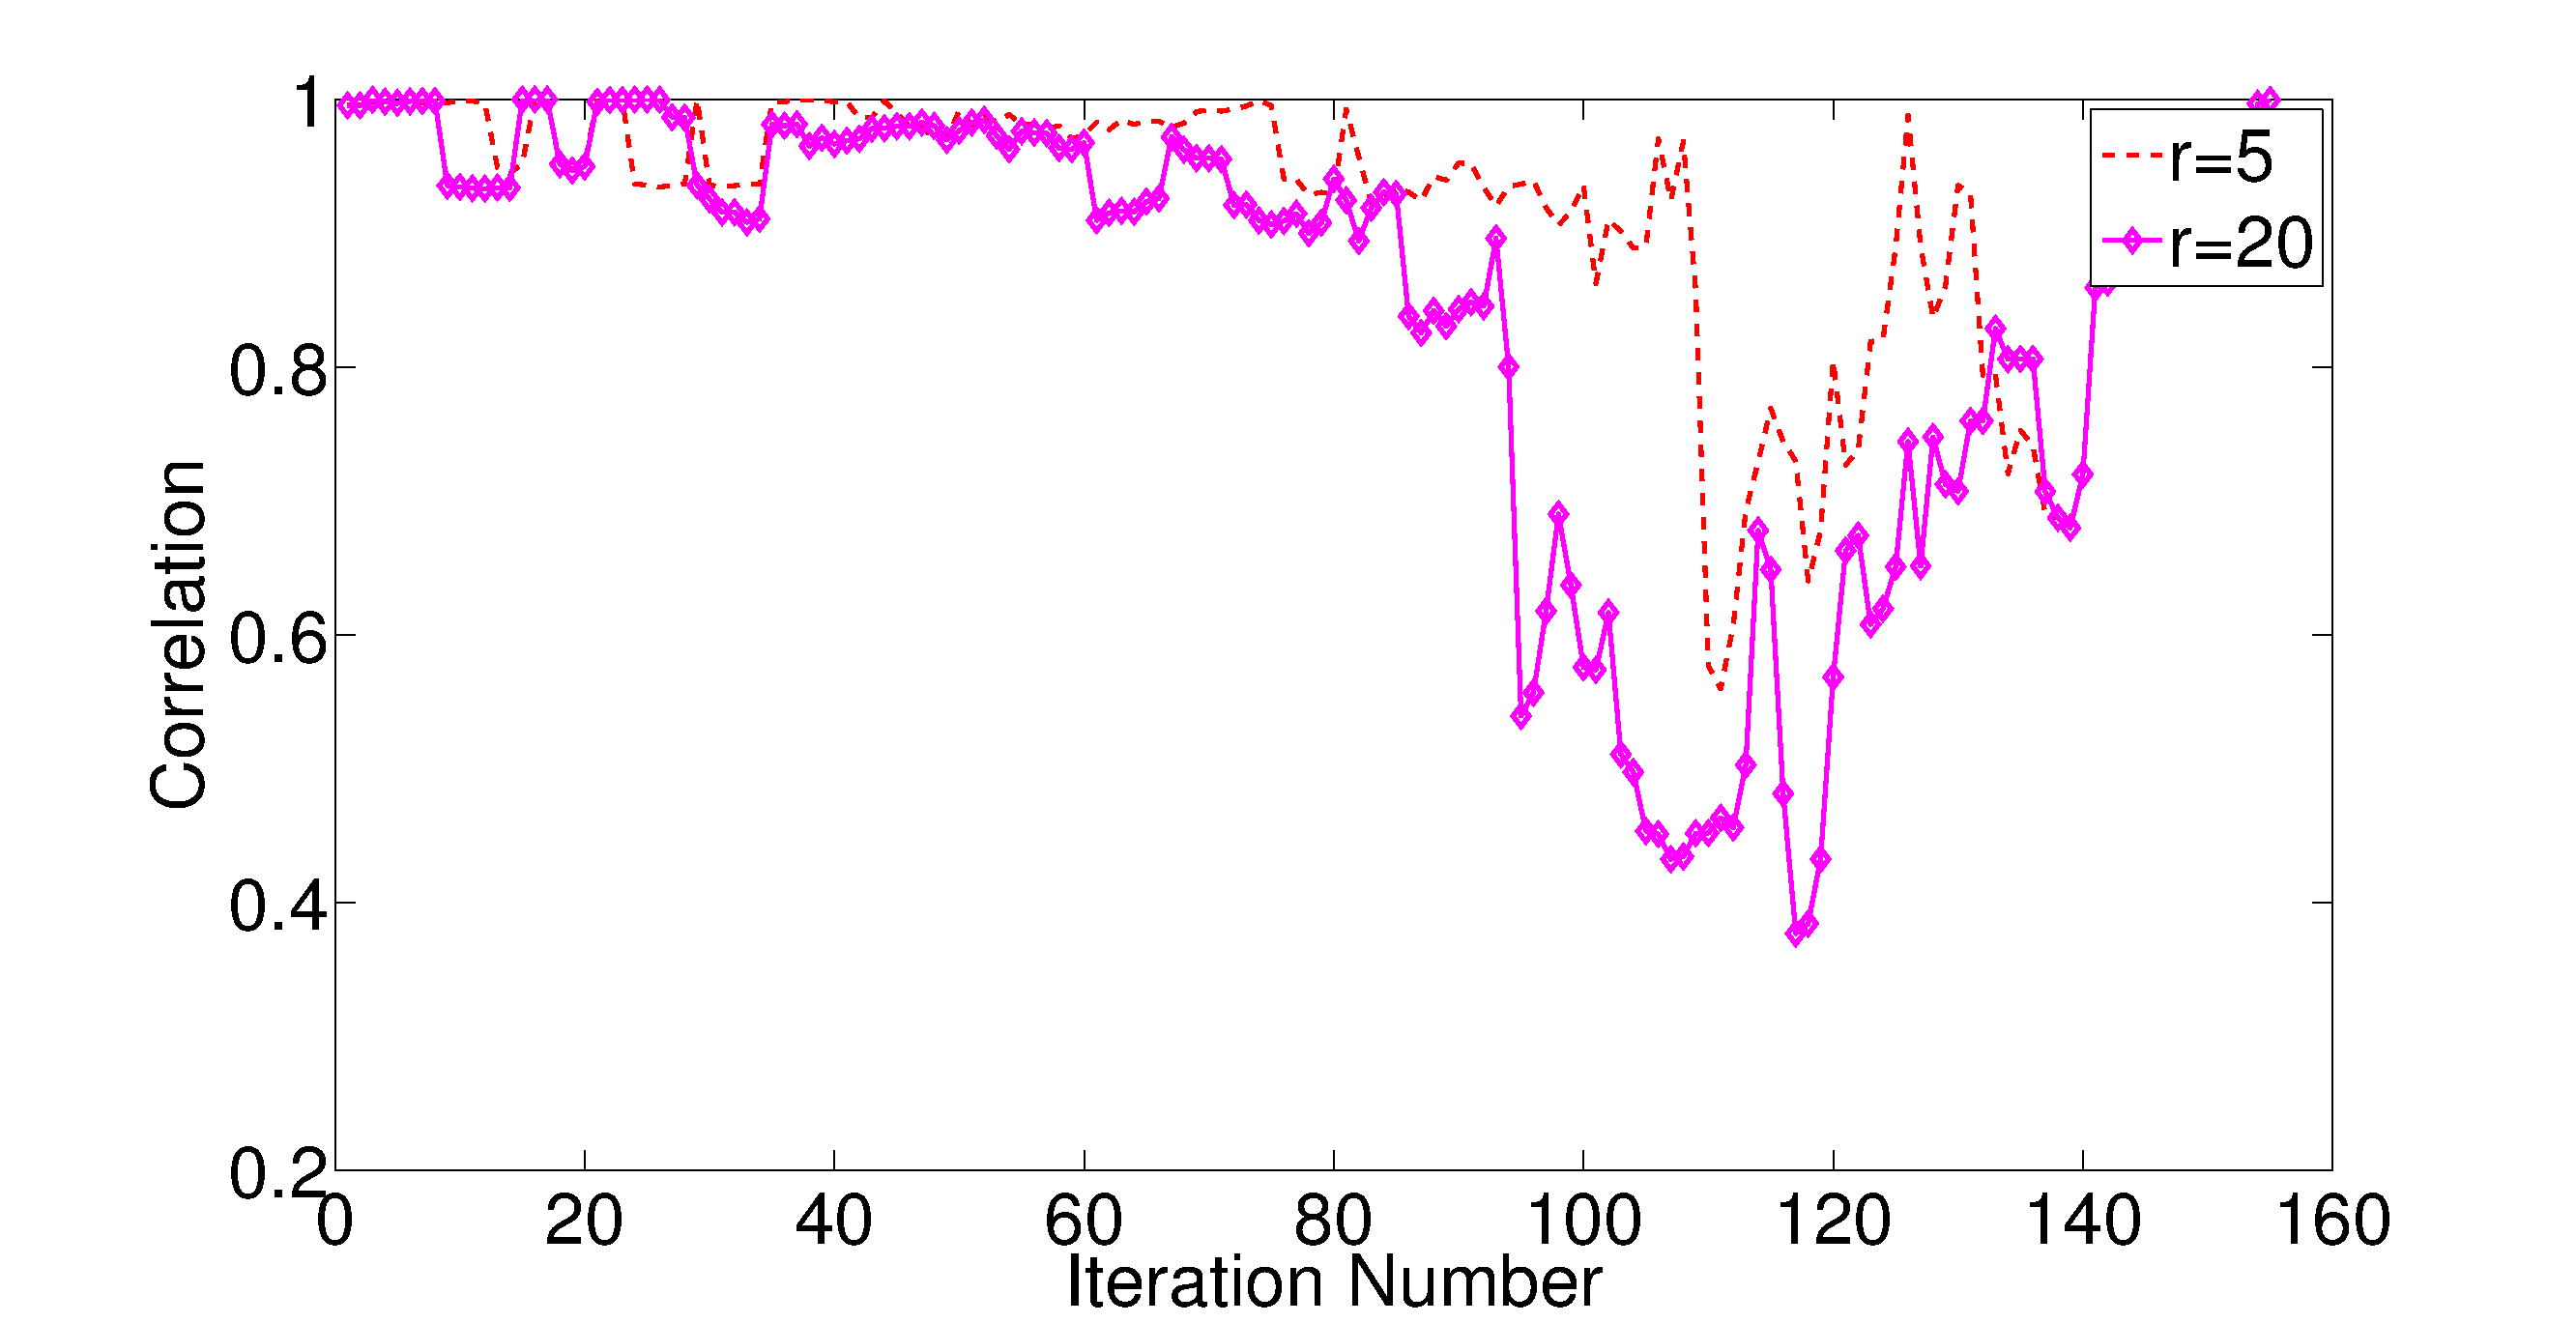
\includegraphics[scale=0.2]{Chapter3/fig/c432_correlation_between_ordering_replacements_with_throwngates.pdf}
\caption{X axis: $i$, Y axis: $\rho(i,i+r)$, where $i$: iteration number and $r$ : number of gate replacements per each iteration for 
\texttt{c432} circuit}
\label{fig:c432-corr}
\end{center}
\end{figure}
\noindent Figure~\ref{fig:c432-corr}
shows the autocorrelation plot of rows of $\pi^{'}$.
The Y-axis shows the correlation and X-axis the iteration number.
Each waveform on this plot shows how the correlation changes in successive iterations.

\noindent From figure~\ref{fig:c432-corr} we see that though there is scope for reducing the runtime by replacing several gates in each iteration, the optimal number of gates $r_{i}^{opt}$ to be replaced in each iteration varies and is not known beforehand. Hence there is a need to define metrics to compute the value of $r_{i}^{opt}$ effectively.\\
\noindent {\bf Observation III:} \\
It is important to note the impact of replacing multiple gates in a single iteration. In order to quantify the impact of replacing multiple gates in a single iteration we define two metrics:

\begin{itemize}
    \item {\it Backtrack (line number $10$ of Algorithm~\ref{alg:naive}) }: In case of a timing violation during a replacement the current replacement needs to be undone and the arrival/required arrival times of all wires in the circuit have to be updated to the old values which it had before the lazy timing update at the end of last iteration. This procedure is referred to as \textit{backtrack}. A large number of backtracks essentially degrades the running time of the TC-DSP optimization algorithm. 

    \item {\it Gate replacement window ($r$) }: In Algorithm~\ref{alg:naive}, only one gate is replaced  with a different $V_t$/$size$ per iteration as seen in line $7$ of the algorithm. This can be increased to $r$ gates. Figure~\ref{fig:saturation-of-running-time} shows the plot of running time versus varying $r$. 
It can be seen here that the running time decreases with an increase in $r$. 
After certain value of $r$ ($r_{opt}$), it saturates and does not improve further. 
        This is because, a very high value of $r$ causes too many backtrack operations thereby saturating the running time of the algorithm. This behavior was observed for other circuits also, although the value of $r_{opt}$ was different 
in each case. In general, the value of $r_{opt}$ increases with the size of the circuit as shown 
in Figure~\ref{fig:ropt}. 
\end{itemize}
\begin{figure}[t]
\begin{center}
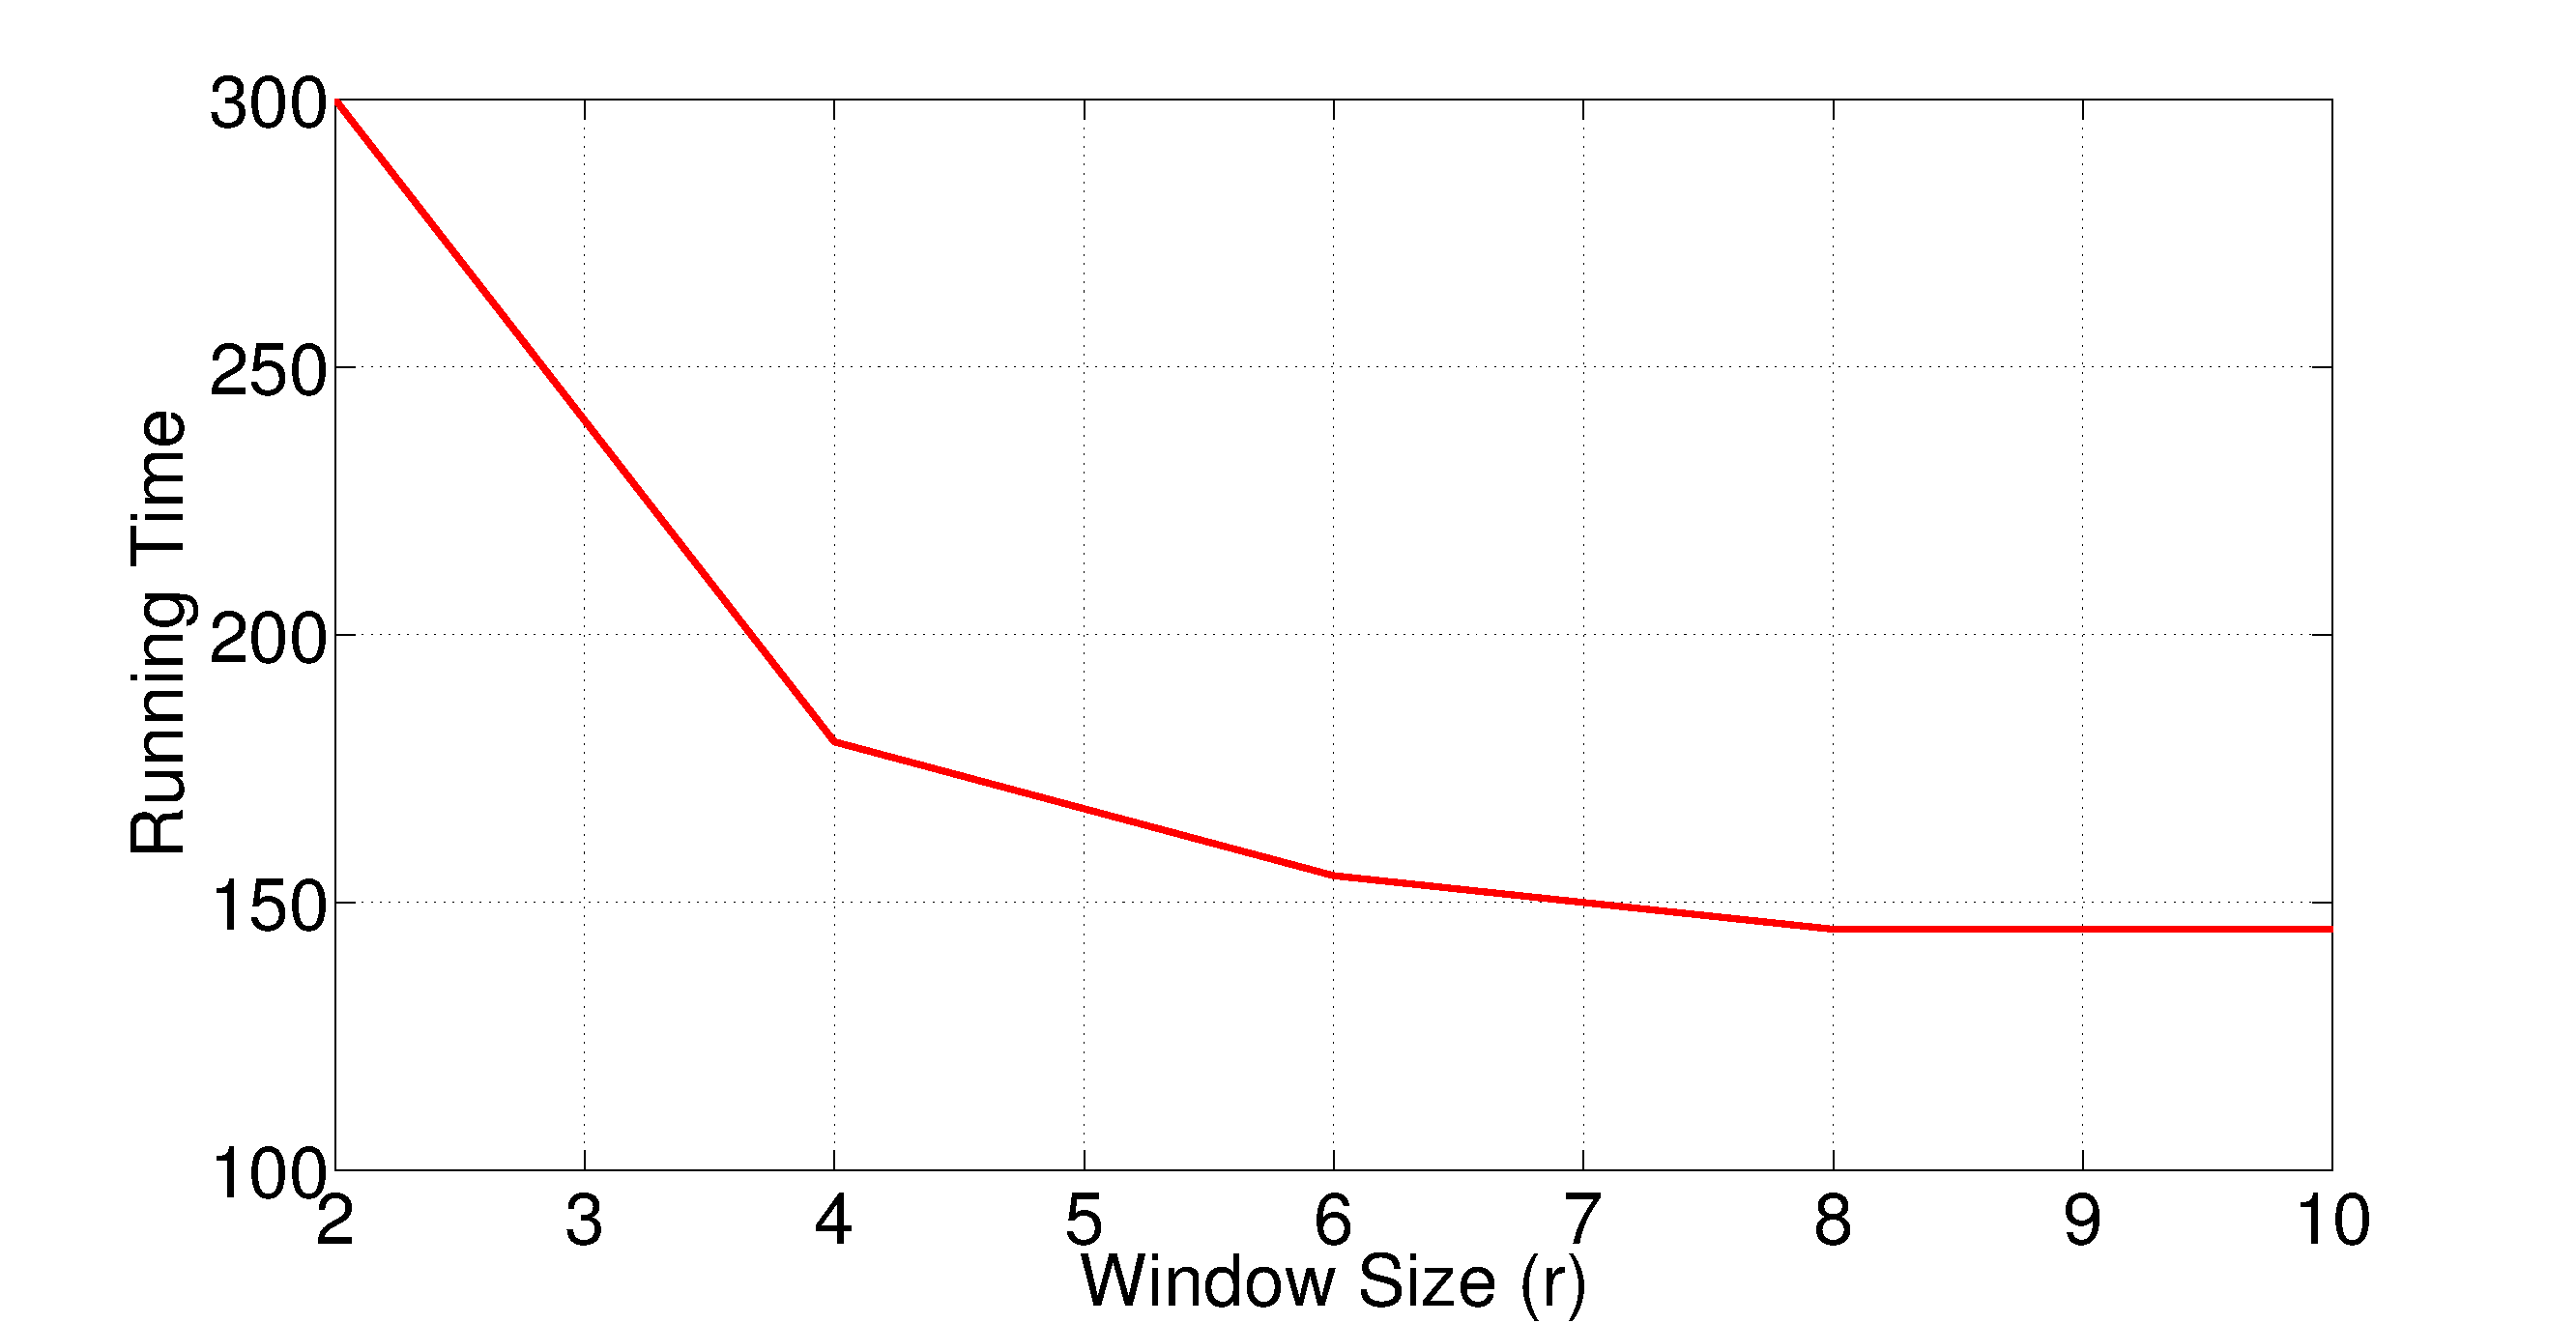
\includegraphics[scale=0.2]{Chapter3/fig/b14_running_time_vs_window_size.pdf}
\end{center}
\caption{Saturation of Running time (in s) with window size for \texttt{b14}}
\label{fig:saturation-of-running-time}
\end{figure}
\begin{figure}[t]
\begin{center}
\vspace{-0.2in}
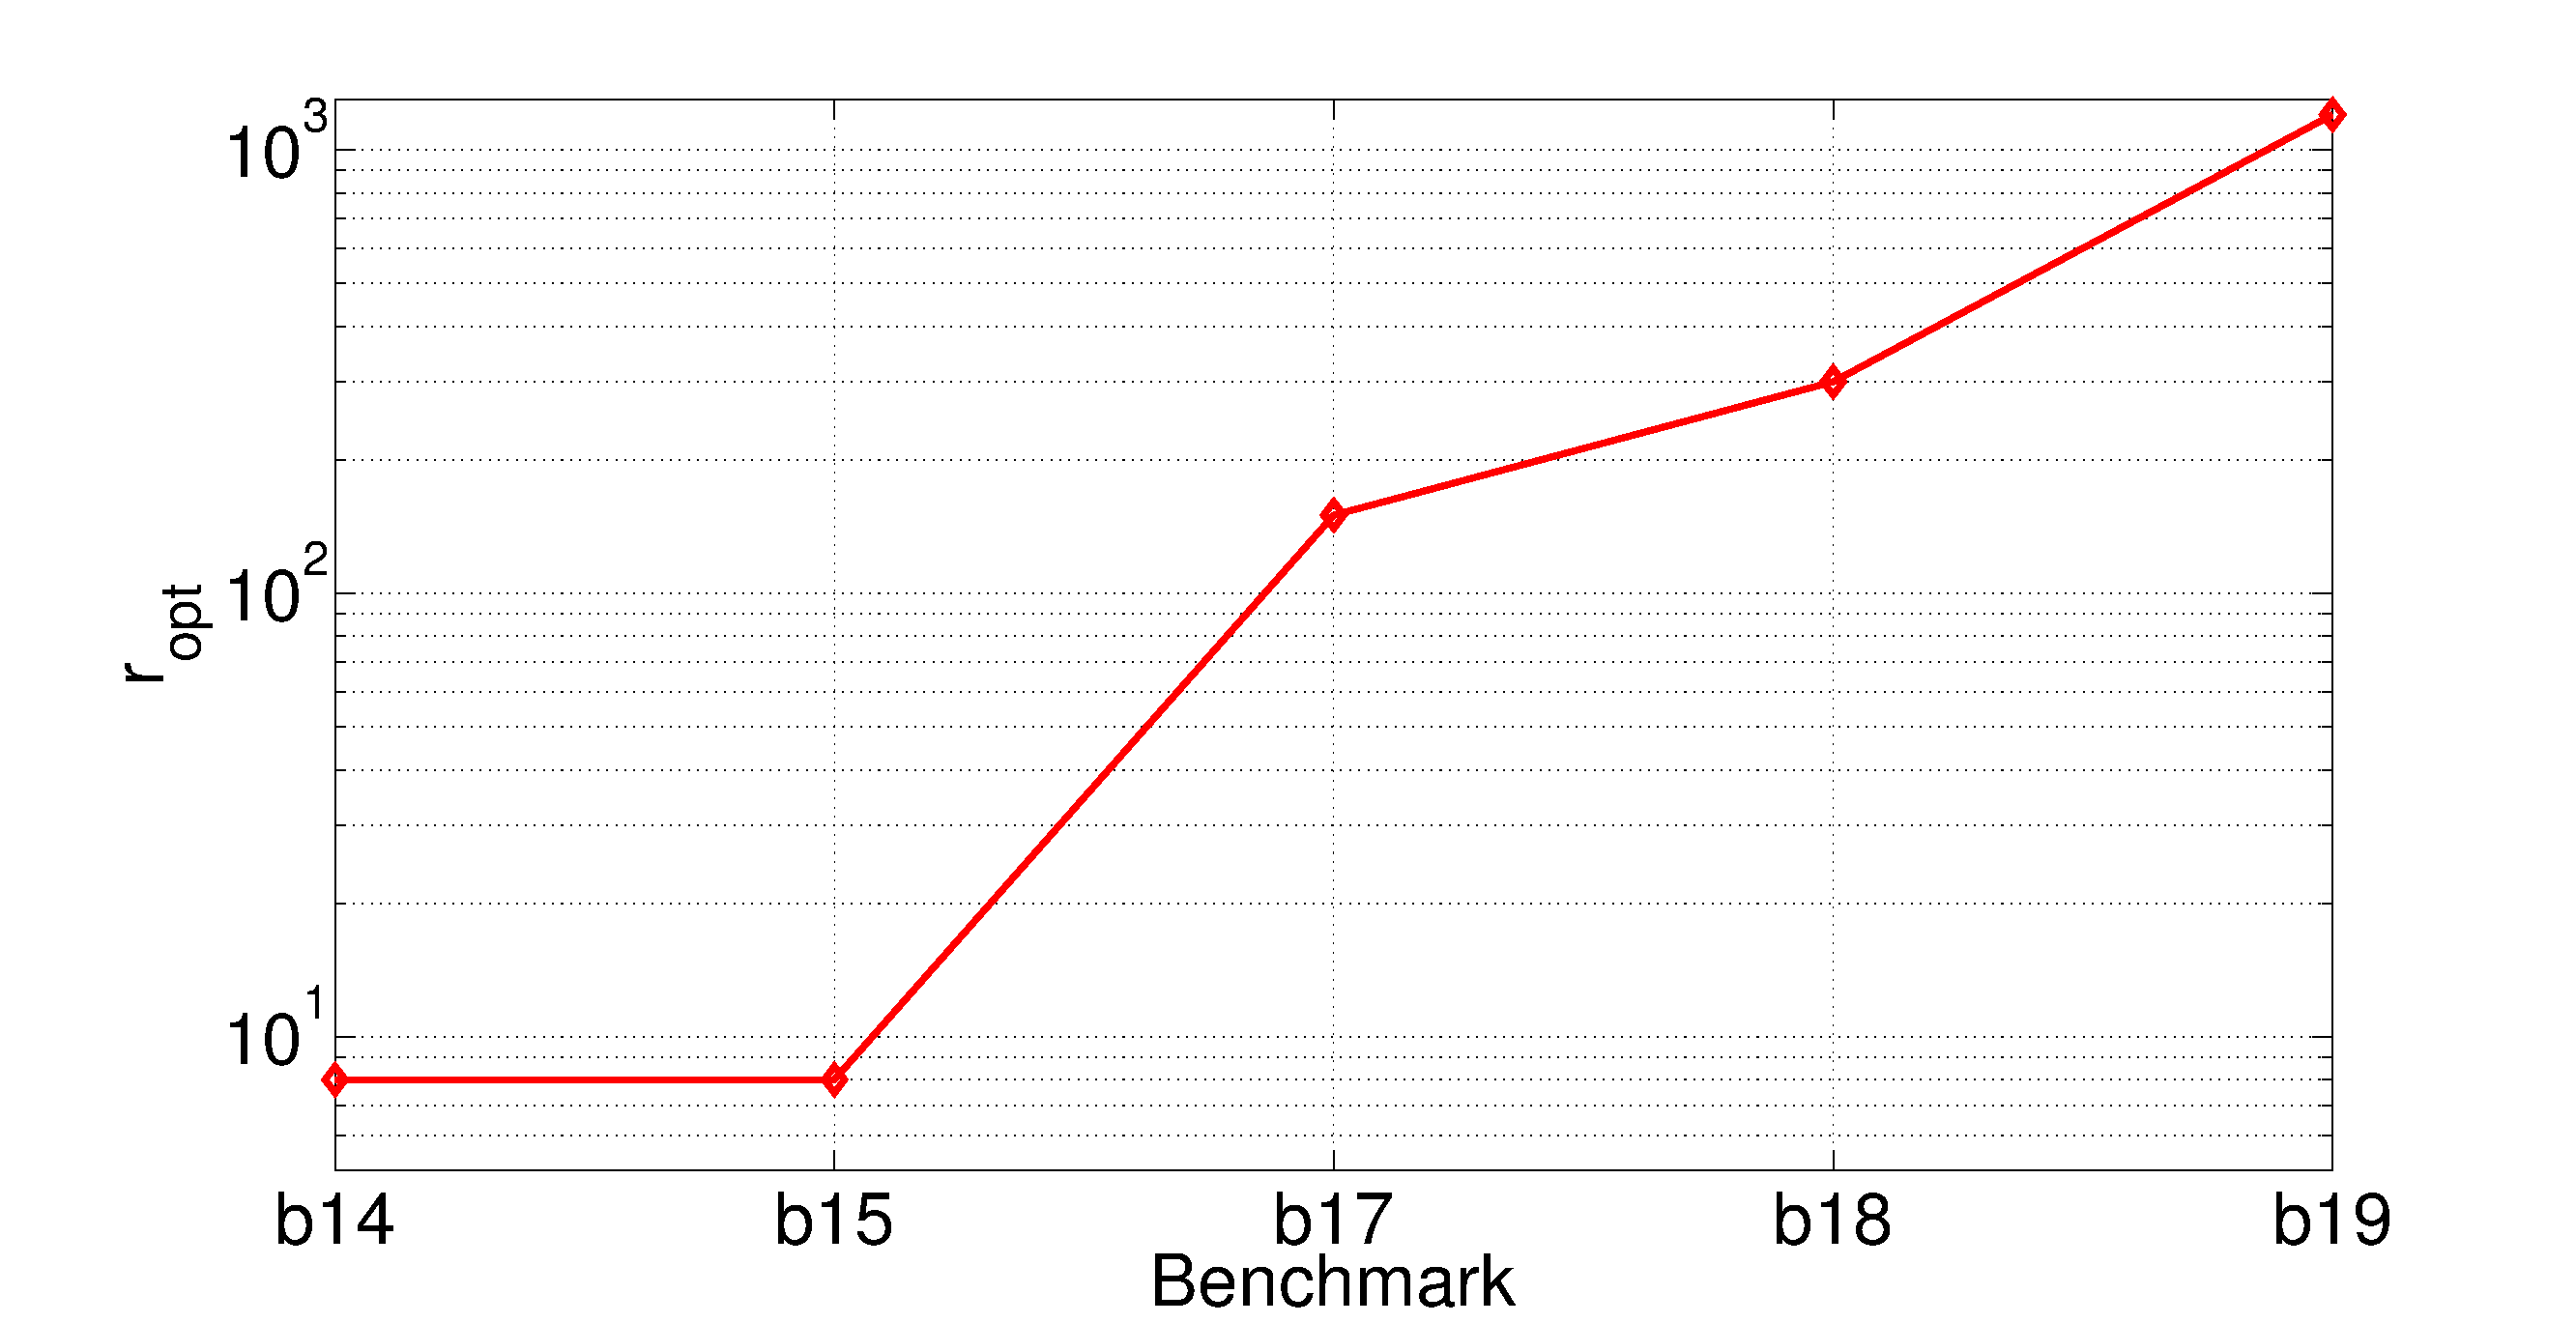
\includegraphics[scale=0.2]{Chapter3/fig/ropt.pdf}
\end{center}
\caption{$r_{opt}$ for different benchmarks}
\label{fig:ropt}
  %}
\caption{Figure showing the impact of varying $r$ over different benchmarks.}
\end{figure}


\noindent Figure~\ref{fig:c432-corr} shows that even for $r=20$, the correlation is very good, providing the opportunity for performing {\it lazy timing updates} between gate replacement iterations. If correlation is good for a certain value of $r$, it indicates that we can replace $r$ gates at a time, without violating timing. However, it impacts the run-time significantly if the iterative correlation is less. Further, it can also be observed in Figure~\ref{fig:c432-corr} that the correlation is not uniform across all iterations. Gates higher up in the ordering considered in the first few iterations have a high degree of correlation, whereas gates considered in the middle exhibit lower correlation. Hence replacing a fixed number of gates for each iteration may not effectively 
exploit the iterative correlation, leading to sub-optimal results. 


\noindent It can also be observed that while performing {\em lazy timing analysis}, an incremental-STA based update needs multiple {\em incremental STA runs}, one for each replacement. For a large $r$ , running one full blown STA (FSTA) run is much more efficient than running $r$ incremental-STA (ISTA) runs, 
to make the lazy timing update. For this reason, FSTA is employed for making the lazy timing updates during the  optimization.

\noindent \textbf{Inference}: The above observations can lead to the following inferences:

\begin{itemize}
\item Multiple gates can be replaced in a single iteration using {\it lazy timing analysis}.
\item It would be desirable to change the number of gates being replaced  in successive iterations, by exploiting the iterative correlation to 
effectively improve the algorithm running time, without compromising the solution quality.
\end{itemize}





\noindent From the above observations and inferences, we understand that a) multiple gates can be replaced 
in a single iteration using {\em lazy timing analysis} and that the optimal window size ($r$) for best 
savings in running time depends on the iteration. The next section explains how to adaptively vary $r$ to obtain the best savings in running time, without impacting solution quality. As seen in Table~\ref{Tab:tab1} we also see that two different circuits, irrespective of their sizes, can have many sub-circuits in common. This indicates that some of the solutions for smaller benchmarks can be reused for the larger benchmarks. However, the final $V_t$ and $size$ choice is dependent on several other factors apart from identical sub-circuits. Hence appropriate features need to be chosen so that the solutions for a benchmark can be leveraged while solving for others. To this end, we propose \textit{MLTimer} which uses the above observations to speed-up the leakage power optimization algorithm while improving the solution quality.

\section{Problem}

\label{sec:problem}

\noindent Consider a circuit $C$ formed using  $N$ gates. Let each of the gate be realizable using $m$ choices made available in the foundry provided standard cell library.\\
Let $p_{i}$ denote the power of the $i^{th}$ cell in the netlist.\\
Let $d_{i}$ denote the delay of the $i^{th}$ cell in the netlist.\\
Let $A_{i}$ denote the input arrival time at the $i^{th}$ cell in the netlist.\\





%Let each of the gate $g_i$ be realizable using several choices of $V_t$ made available in the foundry provided standard-cell library.
 Let $x_{i}^{j}$ denote a discrete variable defined as follows:\\
  \begin{equation}
   {x_{i}^{j}} =
   \left\{
           \begin{array}{lllll}
                  1, \ {\bf if}\ i^{th} gate\  in\ the\ given\ circuit\ is\ realized\\
                  \  \  \ \ with\ j^{th}\ choice\ of\ cell\ in\ the\ standard\ cell\  library\\
                  0, \ {\bf otherwise}\\
          \end{array}
  \right.
  \end{equation}
 
 
 
%
The optimization problem is to find $x_{i}^{j}$ for lowest leakage power, without violating the critical path timing. Let $fanin(i)$ be the set of all gates driving the $i^{th}$ gate.\\
$PO(C)$ and $PI(C)$ denote the set of  primary outputs and  primary inputs respectively of the given circuit $C$; and, $T$ denote the timing budget assigned to $C$.\\
The leakage minimization problem for C can be formally stated as follows:
\begin{equation}\label{opt_eqn_1} {\Large{\underset{}{\operatorname{Minimize}}\sum_{i=1}^{N_{gate}} \sum_{j=1}^{m} x_{i}^{j} p_{i}}}  \end{equation}
\indent \indent \indent \indent \indent such that
\begin{equation}\label{opt_eqn_2} \sum_{j=1}^{m} x_{i}^{j} = 1, \forall i, 1 \leq i \leq N\end{equation}
%\begin{equation}\label{opt_eqn_3}  x_{g_{i,j}} \in \{0,1\}, \forall i, 1 \leq i \leq N_{gate}; \forall j, 1 \leq j \leq m \end{equation}
\begin{equation}\label{opt_eqn_4} A(i) + \sum_{j=1}^{m} d_{i} x_{i}^{j} \le A(k), \forall k \in fanin(i)\end{equation}
\begin{equation}\label{opt_eqn_5} A(O) \le T, \forall O \in PO(C) \end{equation}
\begin{equation}\label{opt_eqn_6} A(I) \ge 0, \forall I \in PI(C)\end{equation}\\



\noindent In the above equations~\ref{opt_eqn_5} and \ref{opt_eqn_6}, $A(O)$ and $A(I)$ denote the arrival-times at primary output wires and primary input wires of C respectively. Equation~\ref{opt_eqn_1} presents the objective function that minimizes the leakage power of the given circuit.
Equation~\ref{opt_eqn_2} ensures that exactly one version of gate $i$ is used among its available $m$ choices.
Equations~\ref{opt_eqn_4}, \ref{opt_eqn_5} and \ref{opt_eqn_6} ensure that the arrival-time constraints are met for all the gates, primary inputs and primary outputs of C respectively. In the next section, we give a detailed account of the related work on the leakage power minimization problem.

\section{The Proposed Algorithm}
\label{sec:proposed}
In this section we detail the working of our proposed \textit{MLTimer} algorithm. The \textit{MLTimer} algorithm consists of the following modules as shown in Figure~\ref{fig:algo}:
\begin{itemize}
    \item \textbf{Learning Module:} This module employs Support Vector Machines (SVM) to predict an initial configuration ($V_t$ and $size$ values) for each gate in the netlist that could ultimately lead to a power and delay optimal solution.
    \item \textbf{Delay Recovery Module:} This module takes the output configuration provided by the learning module and the target delay as inputs. The module then checks the design for any timing violations and fixes them iteratively using Algorithm~\ref{alg:delay}.
    \item \textbf{Leakage Power Recovery Module:} This module uses the solution provided by the delay recovery module to perform leakage optimization.
\end{itemize}

\noindent We now describe the working of each module in detail.

\begin{figure}[!t]
\begin{center}
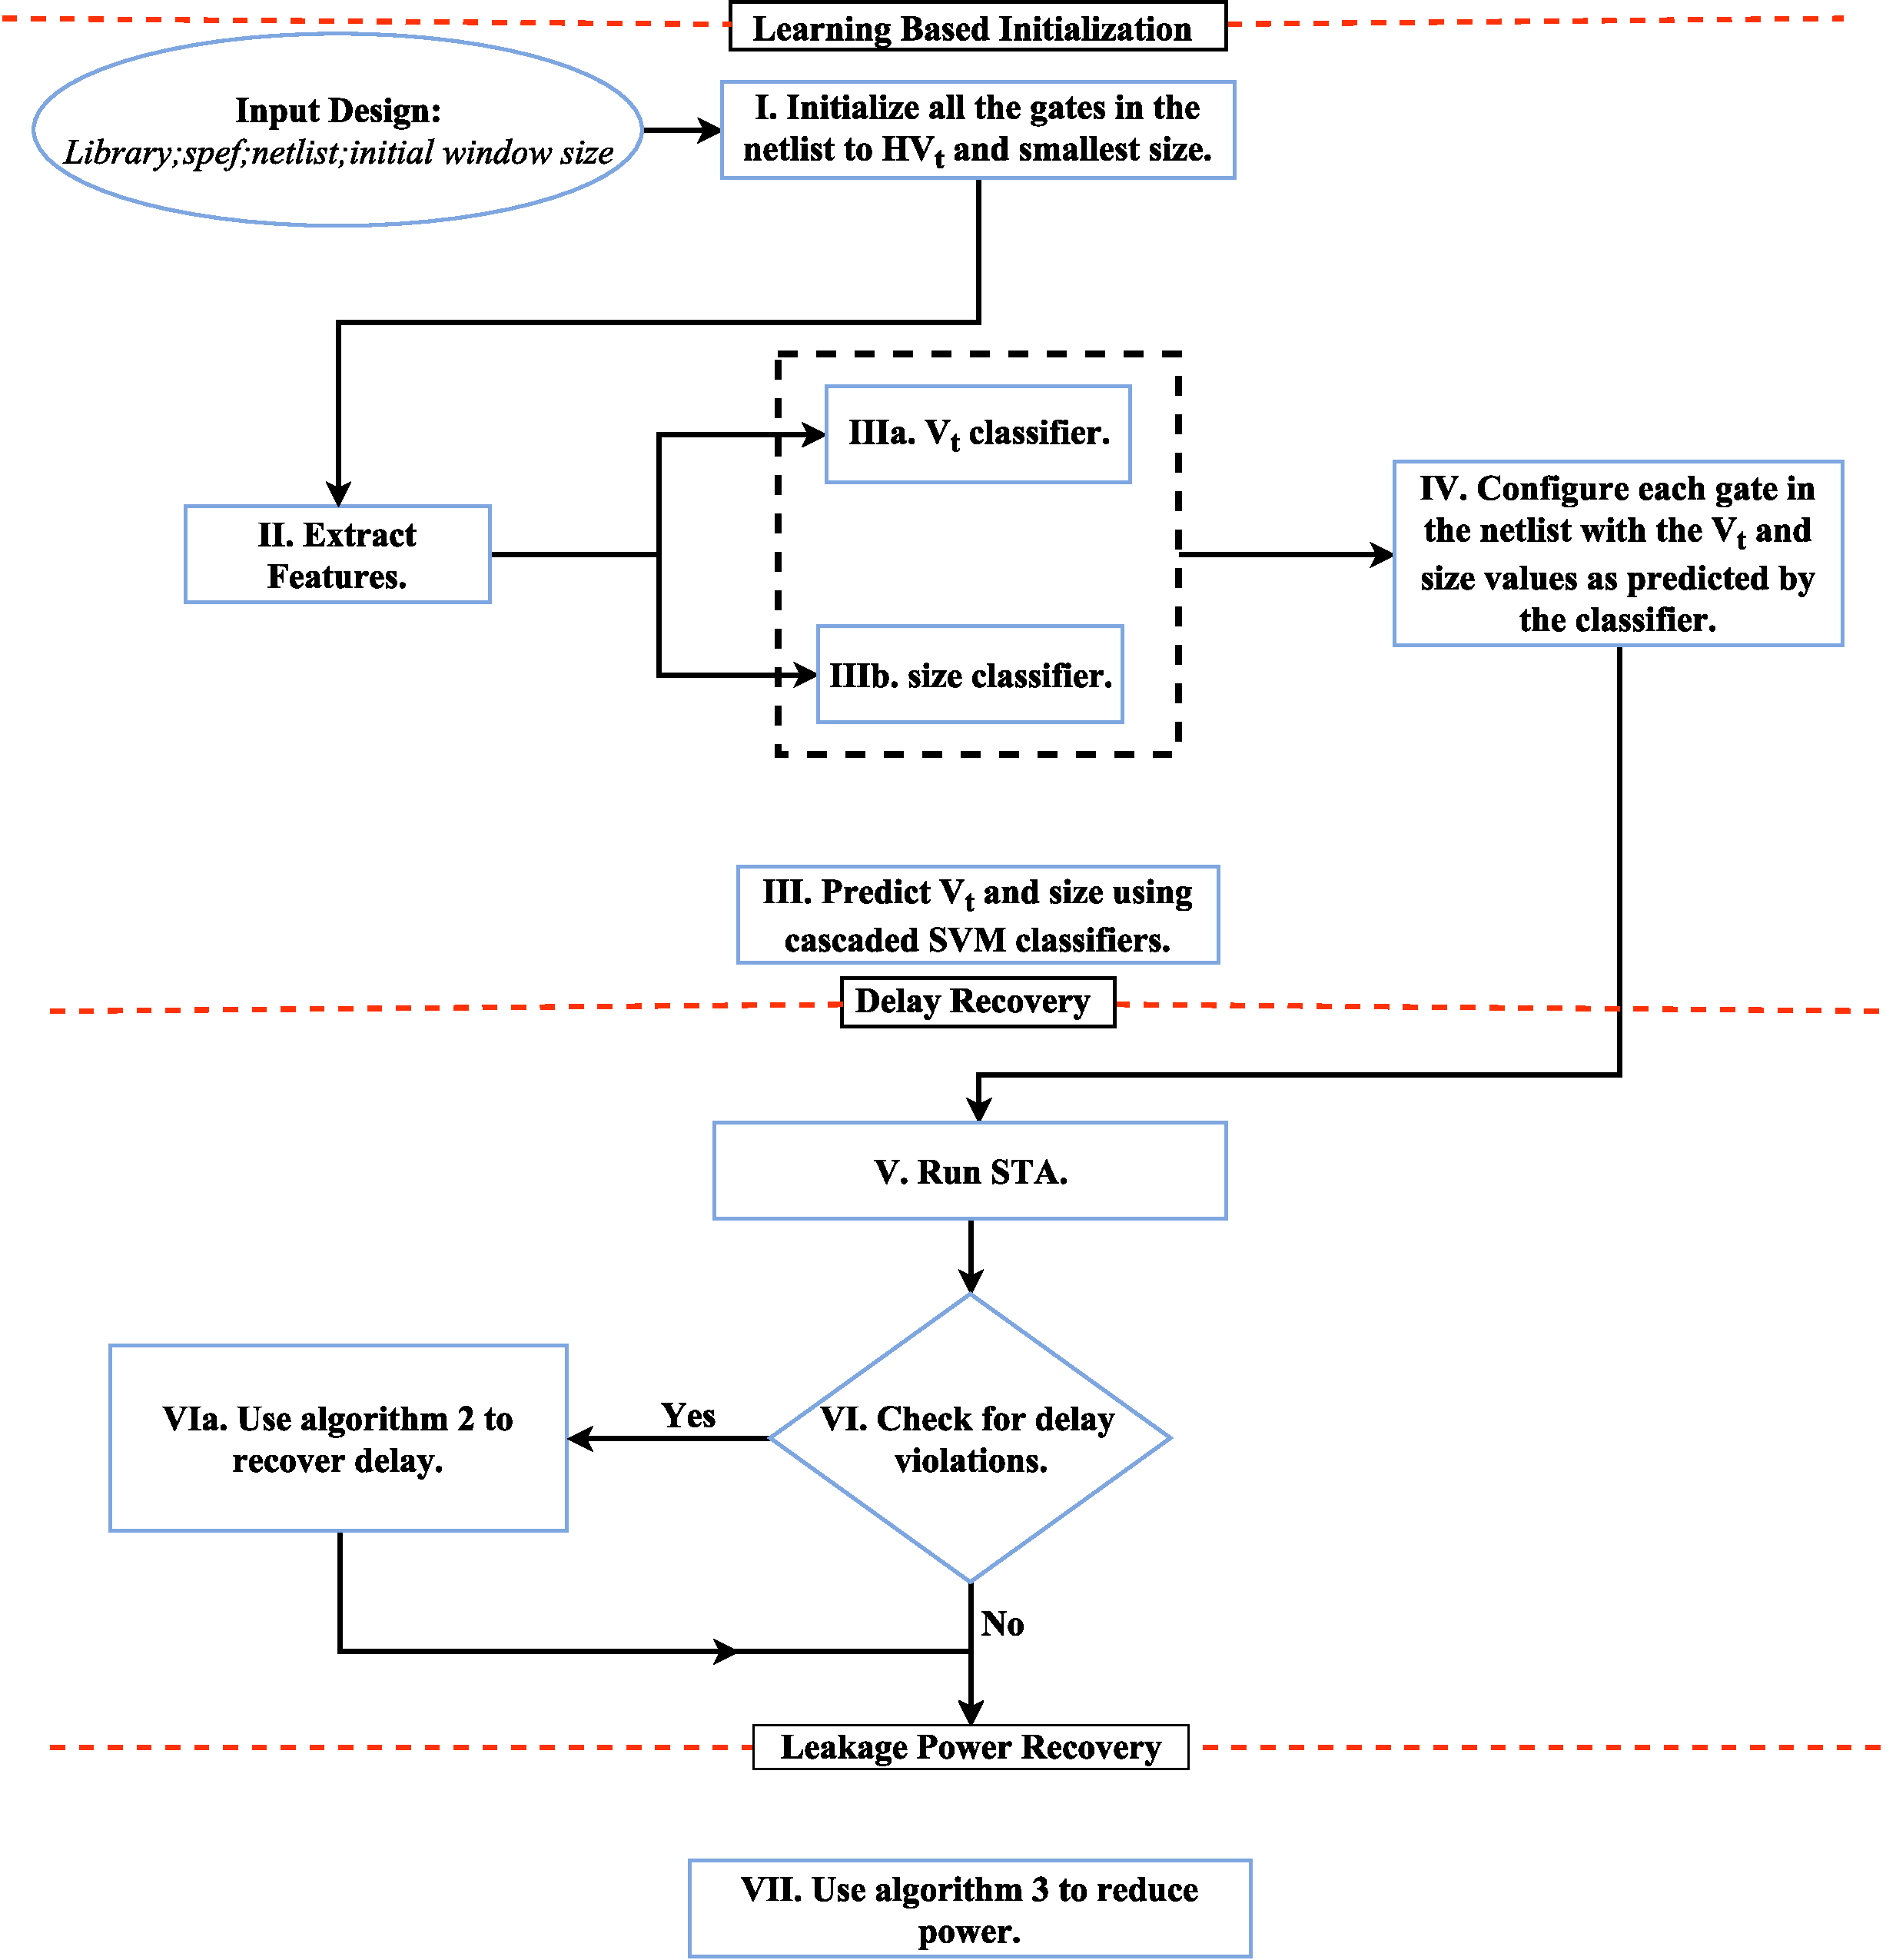
\includegraphics[scale=0.35]{Chapter3/fig/learntimer.pdf}
\caption{The flowchart describes the various steps of our \textit{MLTimer} algorithm.}
\label{fig:algo}
\end{center}
\end{figure}


\subsection{The Learning Module}
\label{sec:feature}
\noindent As seen in Figure~\ref{fig:algo}, the Learning Module takes the netlist initialized to $HV_t$%\footnote{The standard cell library has three available $V_t$ choices. We designate the largest $V_t$ choice as $HV_t$ $(V_t=2)$, the second as $SV_t$ $(V_t=1)$ and the third and smallest choice as $LV_t$ $(V_t=0)$. The largest $V_t$ choice ($V_t=2$) is slower but better in terms of leakage power whereas the smallest ($V_t=0$) is faster but consumes more leakage power. Similarly the library has ten available $size$ choices which we designate as $size=0$, $size=1$ and so on. The gate with the smallest $size$ ($size=0$) is slower but is power efficient and the gate with the largest $size$ ($size=9$) is faster but consumes more power. }
and smallest size as input and predicts a $V_t$ and $size$ value for every gate in the netlist in order to reduce the delay and power. We saw in the previous section that though two netlists are functionally different they might share several common sub-circuits as show in Table~\ref{Tab:tab1}. However, two matching gates belonging to different structurally similar sub-circuits might differ in other aspects. For example, the second circuit might have a tighter timing constraint because of which using the $V_t$ and $size$ values of the first circuit might not improve the delay or the power. Instead it might worsen the power and the delay of the second instance thereby requiring additional iterations of optimization. Enumerating all the features that affect two matching gates and comparing them is prohibitively time consuming. Machine Learning (ML) techniques help in this regard. 
\noindent The initial configuration for each gate in the netlist is predicted using the Support Vector Machines.  Support Vector Machine \cite{SVM} is a highly memory efficient supervised learning technique that is primarily used for classification and outliers detection. An SVM engine takes in the labeled training data and tries to find a separation boundary that correctly separates each data point across dimensions. Figure~\ref{fig:SVM} shows an example of the hyperplane that a typical SVM engine computes. 

\begin{figure}[!t]
 \begin{center}

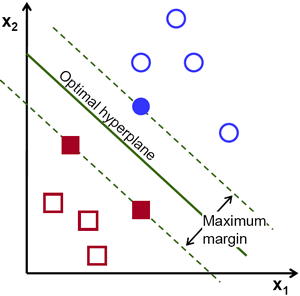
\includegraphics[scale=2]{Chapter3/fig/optimal-hyperplane}
 \caption{An example of the hyperplane/decision boundary that an SVM engine would compute. The SVM engine will take in the data-points (labeled in red and blue) $\times$ features $(X1,X2)$ and try to find the boundary between the data-points across the dimensions. Every feature accounts for one dimension.}
 \label{fig:SVM}
 \end{center}
 \end{figure}
 

 
Since SVM is a supervised learning technique, it needs to be initially trained with a labeled training data. In the first stage, we train two SVM classifiers to predict the $V_t$ and $size$ for each gate in the netlist, respectively. 
 %\subsubsection{Feature selection}
 %
\noindent We saw in Section~\ref{sec:motivation} that the final choice of $V_t$ and $size$ for a gate is not just dependent on its neighbours but on a variety of other design conditions. Hence, we identify seven such design parameters and use them as features for our technique. These features are described below:.
\begin{itemize}
    \item\textbf{  Gate Type}: This represents the functionality of the gate. Each standard cell library has a collection of low-level Boolean functions. For our experiments we use the ISPD contest library which has $13$ gate types. The gate type distribution across the benchmark circuits is shown in Table~\ref{tab:tab2}. 
 \item\textbf{ Sub-circuit}: A sub-circuit $S_i$ of a gate $g_i$ is the set of gates whose timing values are drastically affected by any change in $V_t$/$size$ of gate $g_i$.  For our experiments $S_i$ comprises the immediate fanins and fanouts of $g_i$.
 \item\textbf{ Local Negative Slack (LNS)}: We define LNS of gate $g_i$ ($LNS_i$) as the sum of all the negative slack paths that pass through $g_i$.
 \item\textbf{ Number of Fanins}: This is the number of inputs to the gate $g_i$. It accounts for the impact of modifying the $size$ of a gate $g_i$. Resizing gate $g_i$ might impact all the gates in the fanin cone of $g_i$.
 \item\textbf{ Number of Fanouts}: This is the number of gates driven by $g_i$. A gate with a large number of fanouts cannot be downscaled as it might introduce c.
 \item\textbf{  Number of Negative Slack Paths}: A high value of LNS could be because of i) a large number of negative slack paths passing through the gate $g_i$; or, ii) a small number of paths with extremely negative slack values. This feature helps to distinguish the former from the latter. 
 \item\textbf{ Slack of the Node}: As pointed out in the previous section, the amount of positive slack determines the degree to which the $V_t$ of the gate can be scaled.

\end{itemize}

 \begin{table*}[!ht]
     \caption{The Table shows the distribution of gates across the ISPD2012 benchmark suite and ShaktiC core. We use the gates from \texttt{pci} for training. In column 1, A$\times$B indicates that a gate has $A$ inputs and $B$ outputs.}
\label{tab:tab2}

     %\centering
     \begin{tabular}{|p{2cm}|p{1cm}|p{1.2cm}|p{1.8cm}|p{1cm}|p{1.6cm}|p{1.4cm}|p{1.4cm}|p{1.4cm}|}
\hline
         \textbf{Gate type}   &\texttt{pci}&\texttt{b19}&\texttt{des\_perf}&\texttt{DMA}&\texttt{leon3mp}&\texttt{netcard}&\texttt{vga\_lcd} & \texttt{ShaktiC}\\ \hline
    \texttt{NOT     }& 10,280                & 46,757        & 39,297              & 5,628         & 163,333           & 184,317           & 48,277     & 40,794        \\ \hline
    \texttt{NAND 2$\times$1}& 15,877                & 59,460        & 29,459              & 10,722        & 163,921           & 583,704           & 80,571 & 52,506            \\ \hline
    \texttt{NAND 3$\times$1}& 208                  & 6,267         & 3,930               & 372          & 8,890             & 912              & 192   & 1,387           \\ \hline
    \texttt{NAND 4$\times$1}& 295                  & 8,534         & 3,552               & 547          & 15,454            & 13,836            & 2,278 & 2,368            \\ \hline
    \texttt{NOR 2$\times$1}  & 1,403                 & 37,942        & 16,641              & 2,146         & 29,599            & 24,025            & 2,498   & 31,048           \\ \hline
    \texttt{NOR 3$\times$1}  & 14                   & 89           & 521                & 20           & 26               & 64               & 11          & 855     \\ \hline
    \texttt{NOR 4$\times$1}  & 3                    & 117          & 12                 & 1            & 1                & 6                & 2            & 1,264     \\ \hline
    \texttt{AOI21$\times$1}     & 734                  & 28,821        & 4,610               & 1,228         & 18,875            & 3,850             & 5,296   & 6,260           \\ \hline
    \texttt{AOI22$\times$1}     & 720                  & 14,921        & 919                & 1,886         & 69,817            & 48,792            & 8,449   & 14,447           \\ \hline
    \texttt{OAI21$\times$1}      & 304                  & 8,647         & 3,450               & 471          & 52,855            & 1,384             & 186    & 13,432           \\ \hline
    \texttt{OAI22$\times$1}      & 6                    & 1,119         & 36                 & 88           & 17,581            & 59               & 52       & 10,395         \\ \hline
\texttt{Total gates} & 29,844 &	212,674	& 102,427	& 23,109	& 540,352	& 860,949 &	147,812 & 174,756 \\ \hline
\end{tabular}
\end{table*}


\begin{table}[!ht]
\centering
\caption{The Table shows the percentage distribution of gates across the ISPD2012 benchmark suite and ShaktiC core. We use the gates from \texttt{pci} for training. In column 1, A$\times$B indicates that a gate has $A$ inputs and $B$ outputs.}
\label{tab:tab23}
\begin{tabular}{|l|l|l|l|l|l|l|l|l|}
\hline
Gate type ( percentage) & pci\_bridge & b19   & des\_perf & DMA   & leon3mp & netcard & vga\_lcd  & ShaktiC\\ \hline
    \texttt{NOT     }    & 34.45       & 21.99 & 38.37     & 24.35 & 30.23   & 21.41   & 32.66   & 23.66 \\ \hline
    \texttt{NAND 2$\times$1     }            & 53.2        & 27.96 & 28.76     & 46.4  & 30.34   & 67.8    & 54.51 & 30.04    \\ \hline
    \texttt{NAND 3$\times$1     }   & 0.7         & 2.95  & 3.84      & 1.61  & 1.65    & 0.11    & 0.13  & 0.7   \\ \hline
    \texttt{NAND 4$\times$1     }   & 0.99        & 4.01  & 3.47      & 2.37  & 2.86    & 1.61    & 1.54  & 1.3   \\ \hline
    \texttt{NOR 2$\times$1    }   & 4.7         & 17.84 & 16.25     & 9.29  & 5.48    & 2.79    & 1.69   & 17.77  \\ \hline
    \texttt{NOR  3$\times$1   }   & 0.05        & 0.04  & 0.51      & 0.09  & 0       & 0.01    & 0.01  & 0.49   \\ \hline
    \texttt{NOR  4$\times$1   }   & 0.01        & 0.06  & 0.01      & 0     & 0       & 0       & 0    &  0.72   \\ \hline
    \texttt{AOI  21$\times$1   }   & 2.46        & 13.55 & 4.5       & 5.31  & 3.49    & 0.45    & 3.58  & 3.58   \\ \hline
    \texttt{AOI   22$\times$1  }   & 2.41        & 7.02  & 0.9       & 8.16  & 12.92   & 5.67    & 5.72   & 8.27  \\ \hline
    \texttt{OAI 21$\times$1    }   & 1.02        & 4.07  & 3.37      & 2.04  & 9.78    & 0.16    & 0.13  & 7.69 \\ \hline
    \texttt{OAI  22$\times$1   }   & 0.02        & 0.53  & 0.04      & 0.38  & 3.25    & 0.01    & 0.04  & 5.95   \\ \hline
\end{tabular}
\end{table}

 
 \begin{table}[!ht]
     \caption{These Tables show the number of gates for each $V_t$ and $size$ in the training dataset obtained from the \texttt{pci} benchmark. It can be seen that the number of gates at $LV_t$ and $SV_t$ are much less compared to the number of $HV_t$ gates. This problem is commonly referred to as class imbalance in Machine Learning. From the fifth and sixth rows of the Table we can see that this problem exists for $size$ also.}
\label{tab:dist}

     \centering

\begin{tabular}{ll}
\begin{tabular}{|l|l|l|l|}
\hline
\multicolumn{2}{|l|}{$V_t$}              & \multicolumn{2}{l|}{Percentage of gates} \\ \hline
\multicolumn{2}{|l|}{$V_t = 0$ $(LV_t)$} & \multicolumn{2}{l|}{8.47}                \\ \hline
\multicolumn{2}{|l|}{$V_t=1$ $(SV_t)$}   & \multicolumn{2}{l|}{1.86}                \\ \hline
\multicolumn{2}{|l|}{$V_t=2$ $(HV_t)$}   & \multicolumn{2}{l|}{89.97}               \\ \hline
\end{tabular}
&
\begin{tabular}{|l|l|l|l|}
\hline
\multicolumn{2}{|l|}{$size$}              & \multicolumn{2}{l|}{Percentage of gates} \\ \hline
\multicolumn{2}{|l|}{0} & \multicolumn{2}{l|}{84.40}                \\ \hline
\multicolumn{2}{|l|}{1}   & \multicolumn{2}{l|}{13.75}                \\ \hline
\multicolumn{2}{|l|}{2}   & \multicolumn{2}{l|}{0.7}               \\ \hline
\multicolumn{2}{|l|}{3}   & \multicolumn{2}{l|}{0.7}               \\ \hline
\multicolumn{2}{|l|}{4}   & \multicolumn{2}{l|}{0.2}               \\ \hline
\multicolumn{2}{|l|}{$> 5$}   & \multicolumn{2}{l|}{0.25}               \\ \hline
\end{tabular}
\end{tabular}
\end{table}

\noindent There is no empirical/analytical technique to prove that the above features are comprehensive but they are good indicators as to what might happen to the chosen gate. For example, a gate with extremely high fanout count is highly unlikely to be downsized though it might have high positive slack because the downsizing may lead to capacitance violations. We extract these features for every gate in the netlist. We represent each gate in the netlist along with its associated features  as a matrix. In the training phase, each row in the matrix is associated with a $V_t$ and $size$ label. In the testing phase, the matrix is provided as the input to the trained SVMs that predict a $V_t$ and $size$ value for each gate in the netlist. 


% Please add the following required packages to your document preamble:
% \usepackage{booktabs}
% \usepackage{multirow}
% \begin{figure*}[!t]
%  \begin{center}

% 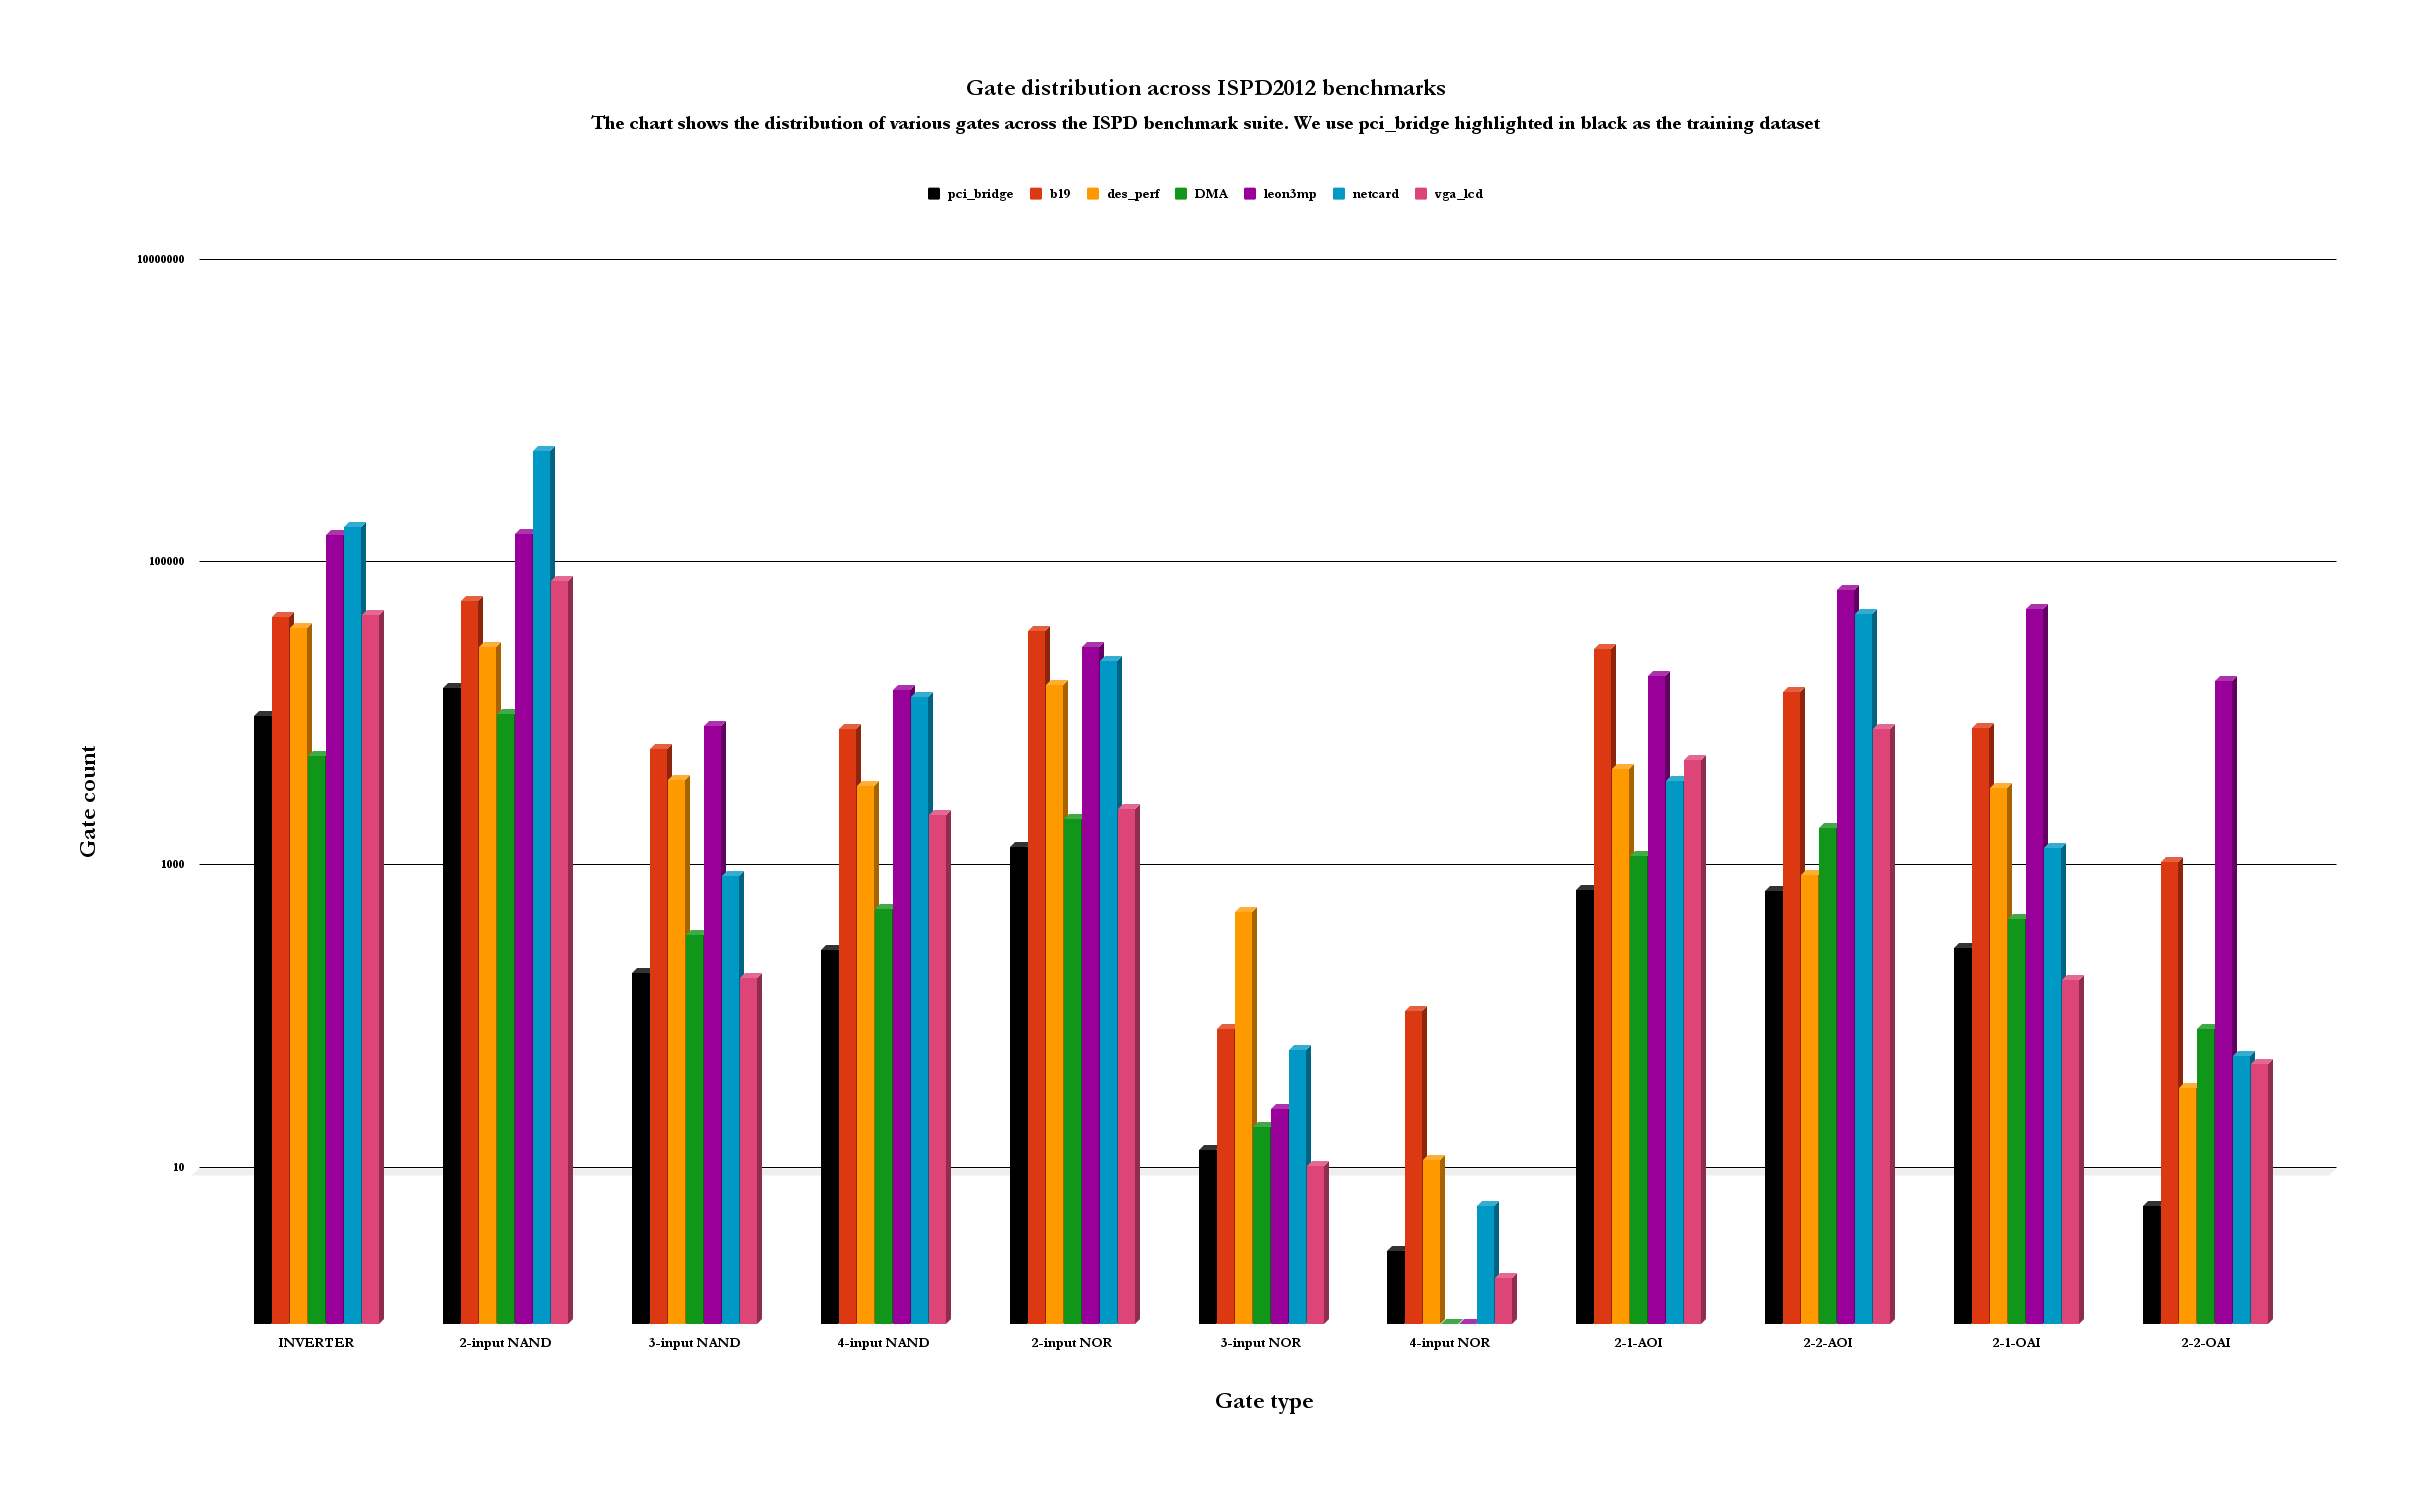
\includegraphics[scale=0.2]{fig/chart1}
%  \caption{An example of the hyperplane/decision boundary that an SVM engine would compute. The SVM engine will take in the data-points(labeled in red and blue) $\times$ features (X1,X2) and try to find the boundary between the data-points across the dimensions (one feature==one dimension).}
%  \label{fig:dist2}
%  \end{center}
%  \end{figure*}
 

% \begin{table*}[!t]
% \begin{minipage}{0.1\linewidth}
% \centering

% \begin{tabular}{|l|l|l|l|l|l|l|l|l|l|l|l|l|}
% \hline
% Gate type   & NOT & \begin{tabular}[c]{@{}l@{}}2-input\\ NAND\end{tabular} & \begin{tabular}[c]{@{}l@{}}3-input\\ NAND\end{tabular} & \begin{tabular}[c]{@{}l@{}}4-input\\ NAND\end{tabular} & \begin{tabular}[c]{@{}l@{}}2-input\\ NOR\end{tabular} & \begin{tabular}[c]{@{}l@{}}3-input\\ NOR\end{tabular} & \begin{tabular}[c]{@{}l@{}}4-input\\ NOR\end{tabular} & \begin{tabular}[c]{@{}l@{}}2-1-AOI\end{tabular} & \begin{tabular}[c]{@{}l@{}}2-2-AOI\end{tabular} & \begin{tabular}[c]{@{}l@{}}2-1-OAI\end{tabular} & \begin{tabular}[c]{@{}l@{}}2-2-OAI\end{tabular} & Total  \\ \hline
% b19         & 46757    & 59460                                                  & 6267                                                   & 8534                                                   & 37942                                                 & 89                                                    & 117                                                   & 28821                                                         & 14921                                                         & 8647                                                          & 1119                                                          & 212674      \\ \hline
% des\_perf   & 39297    & 29459                                                  & 3930                                                   & 3552                                                   & 16641                                                 & 521                                                   & 12                                                    & 4610                                                          & 919                                                           & 3450                                                          & 36                                                            & 102427      \\ \hline
% DMA         & 5628     & 10722                                                  & 372                                                    & 547                                                    & 2146                                                  & 20                                                    & 1                                                     & 1228                                                          & 1886                                                          & 471                                                           & 88                                                            & 23109       \\ \hline
% leon3mp     & 163333   & 163921                                                 & 8890                                                   & 15454                                                  & 29599                                                 & 26                                                    & 1                                                     & 18875                                                         & 69817                                                         & 52855                                                         & 17581                                                         & 540352      \\ \hline
% netcard     & 184317   & 583704                                                 & 912                                                    & 13836                                                  & 24025                                                 & 64                                                    & 6                                                     & 3850                                                          & 48792                                                         & 1384                                                          & 59                                                            & 860949      \\ \hline
% pci\_bridge & 10280    & 15877                                                  & 208                                                    & 295                                                    & 1403                                                  & 14                                                    & 3                                                     & 734                                                           & 720                                                           & 304                                                           & 6                                                             & 29844       \\ \hline
% vga\_lcd    & 48277    & 80571                                                  & 192                                                    & 2278                                                   & 2498                                                  & 11                                                    & 2                                                     & 5296                                                          & 8449                                                          & 186                                                           & 52                                                            & 147812      \\ \hline
% \end{tabular}
% \caption{This table shows the distribution of gates in each ISPD benchmark. We chose pci as it has a uniform distribution of gates. }
% \label{tab:dist2}
% \end{minipage}
% \end{table*}

We use the \texttt{pci} benchmark for generating the training data. It has approximately $30,000$ gates. We use both the slow and fast variants to generate around $60,000$ samples for training the two classifiers. We implemented a greedy replacement heuristic and used it to generate the $V_t$ and $size$ for each gate of all the benchmarks used for training and validating the classifiers. Table~\ref{tab:dist} shows the distribution of the training data-points across $V_t$ and $size$. The aim of the classifier is to predict a good initial configuration which the leakage and delay  steps can use to reach an optimal solution quickly. It is crucial to identify the right set of gates that need to be swapped in order to reach the target solution. 

Since SVM is a supervised learning process, the efficiency of the classifier is highly dependent on the number and nature of training examples. Interestingly we see from Table~\ref{tab:dist} that though the total number of examples available is quite high, the number of gates that need to be swapped from their initial configuration are few in number. These are the gates that are of interest to us as they help in identifying the conditions to swap the $V_t$/$size$ of a gate. It can be seen in Table~\ref{tab:dist} that  we only need to swap very few gates $(\approx20\%)$ to reach an optimal configuration for \texttt{pci} benchmark from which we gather our training data. As a result there are less number of datapoints belonging to $LV_t (V_t=0)$ and $SV_t (V_t=1)$ and a similar observation is also true for $size\geq1$. Thus we see that there is a skew in the nature of datapoints available for training. This skew in the dataset is referred to as \textit{class imbalance}. We resolve the class imbalance by the following two techniques:



\begin{itemize}
    \item\textbf{ Use a cascaded classifier}: Cascaded classification is an ensemble learning technique, wherein multiple instances of the classifiers are used to predict the final class label. Instead of treating the problem as a multi-class classification problem we reduce it to a binary classification problem. We construct a series of classifiers for both $V_t$ and $size$. The cascaded classifier architecture is shown in Figure~\ref{fig:vtsvm}. The cascaded classifier setup works as follows: The first stage of the classifier is trained to classify a given datapoint as $HV_t (V_t=2)$ or not $HV_t (V_t< 2)$. If a gate is classified as not $HV_t (V_t<2)$ then it is given as an input to the subsequent stage which determine if the gate is $LV_t (V_t=0)$ or $SV_t (V_t=1)$. We follow a similar procedure for building the SVM that predicts the ${size}$. The  advantage in using a cascaded setup is that the features in each stage can be fine-tuned to perform well for only a specific $V_t$/$size$ which is easier than fine-tuning the features for all the $V_t$s or $sizes$. 
    In order to determine the accuracy of the output class we use a thresholding function. The thresholding function is based on the class probability of the classifier. If the classifier assigns a class-label at random then the class probability will be approximately equal to $0.5$. A value greater than $0.5$ indicates that the predicted $V_t$/$size$ was not randomly assigned. Thus, the class probability is a good metric to determine the accuracy of the classifier. The thresholding function is a hyper-parameter that can be individually tuned for each stage in the cascaded setup. 
\begin{figure*}[!t]
 \begin{center}
 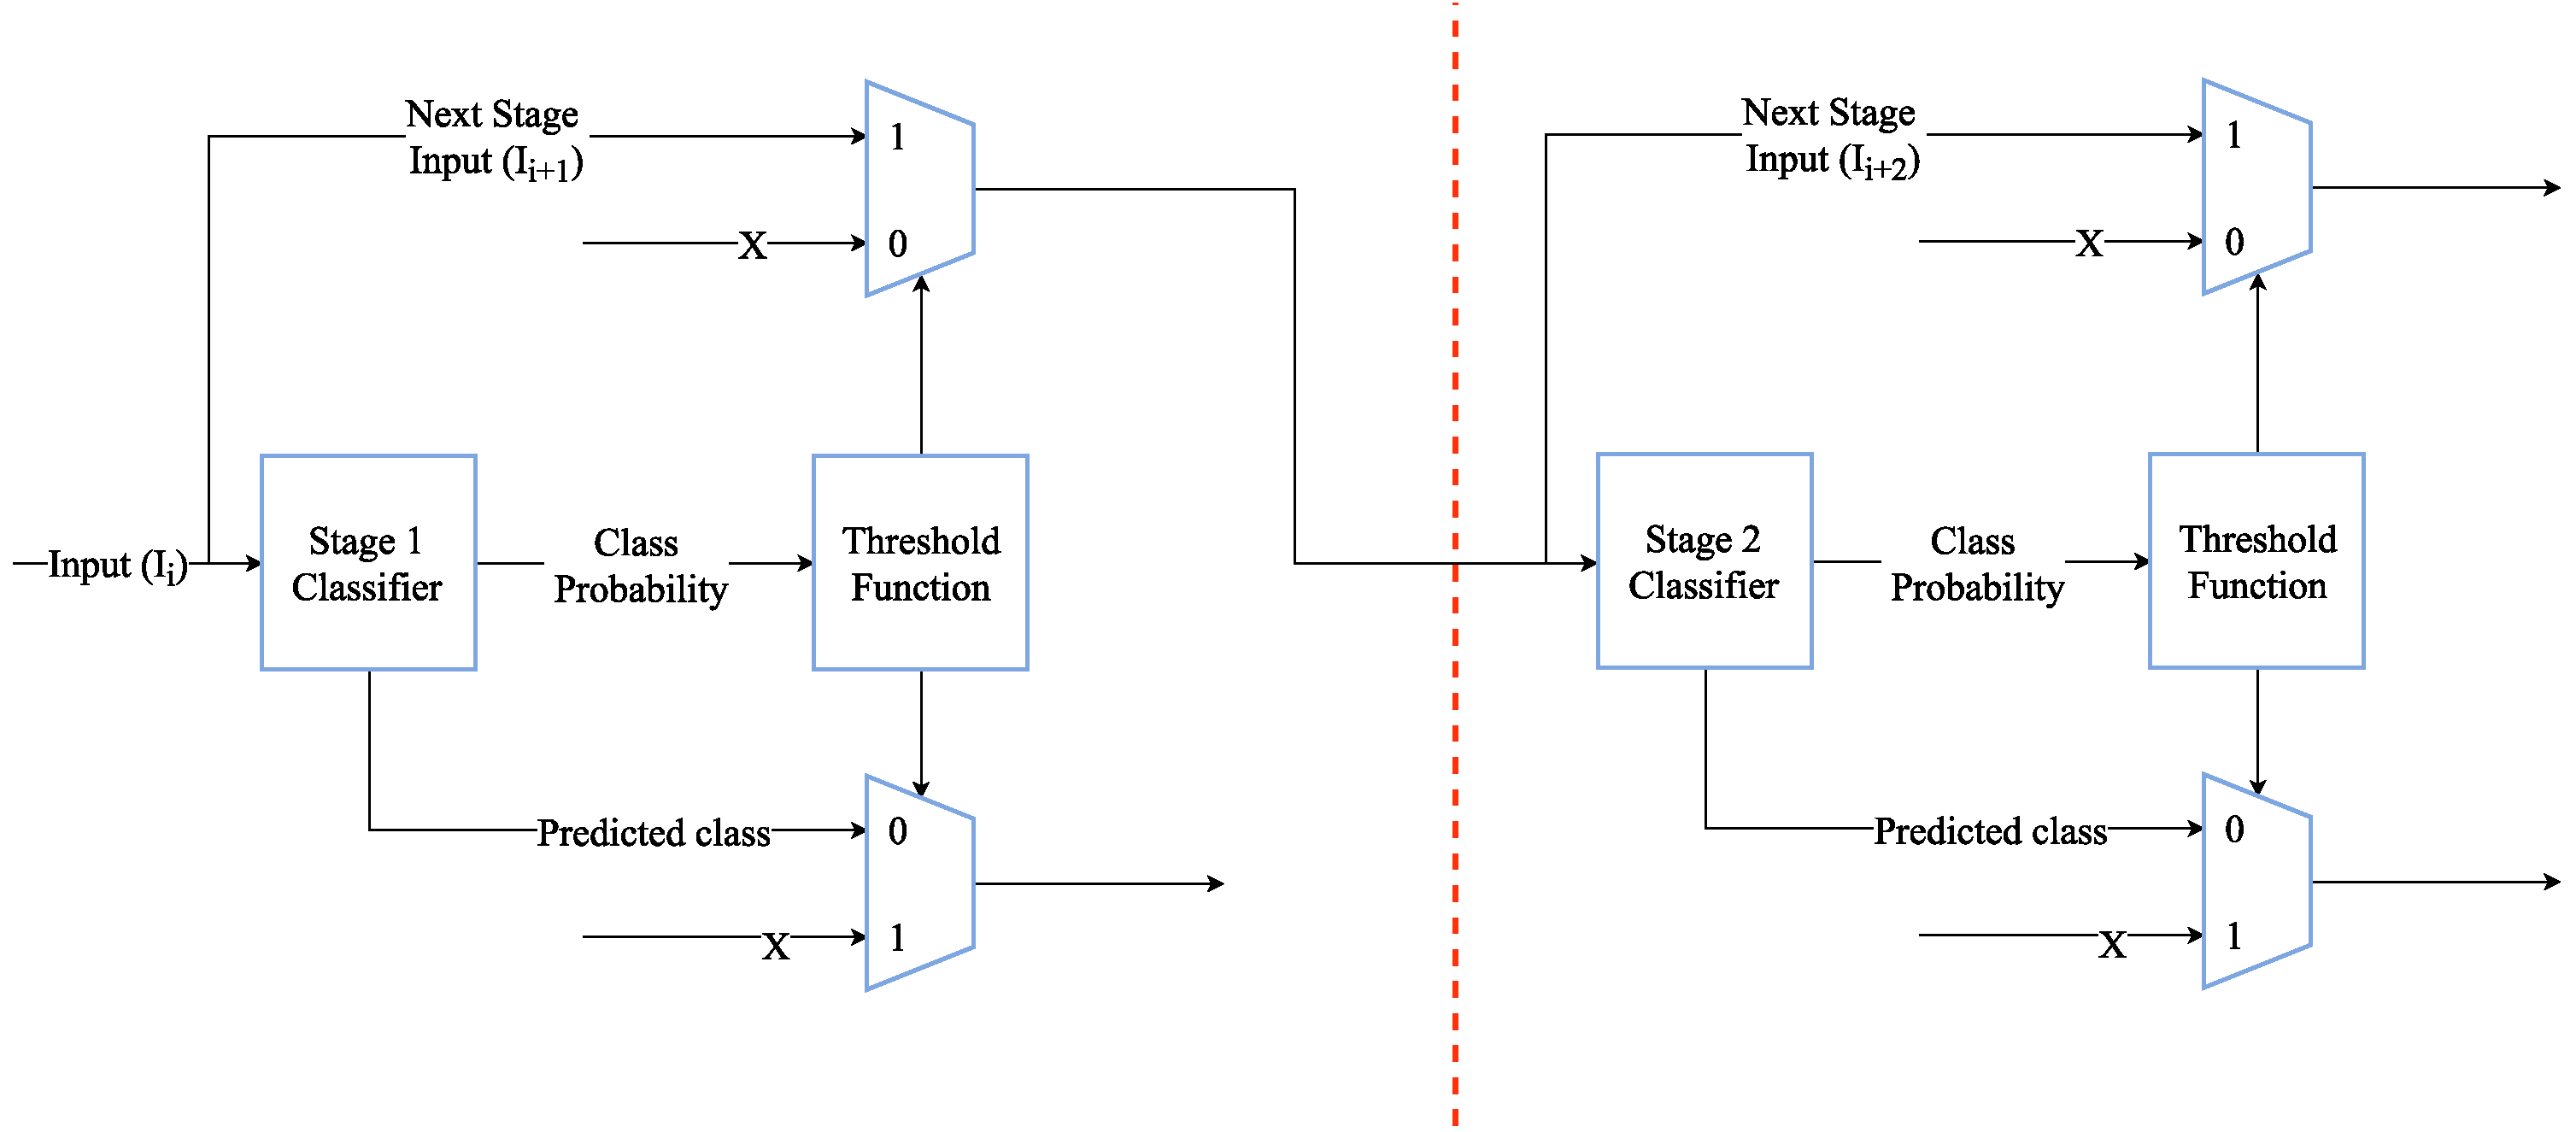
\includegraphics[scale=0.3]{Chapter3/fig/flowchart.pdf}
 \caption{Hierarchical SVM $V_t$ classifier. The first stage $V_t$ classifier classifies the points as $HV_t$ ($V_t = 2 $) or not $HV_t$ ($V_t < 2$) using the thresholding function $T_1$. If the data-point is predicted as not $HV_t$ then it is forwarded to the second stage classifier which uses the thresholding function $T_2$ to classify them as $SV_t$ ($V_t = 1$) and $LV_t$ ($V_t = 0$). The hierarchical $size$ classifier has $5$ -stages.}
 \label{fig:vtsvm}
 \end{center}
 \end{figure*}
%\begin{figure}[!t]
% \begin{center}
% 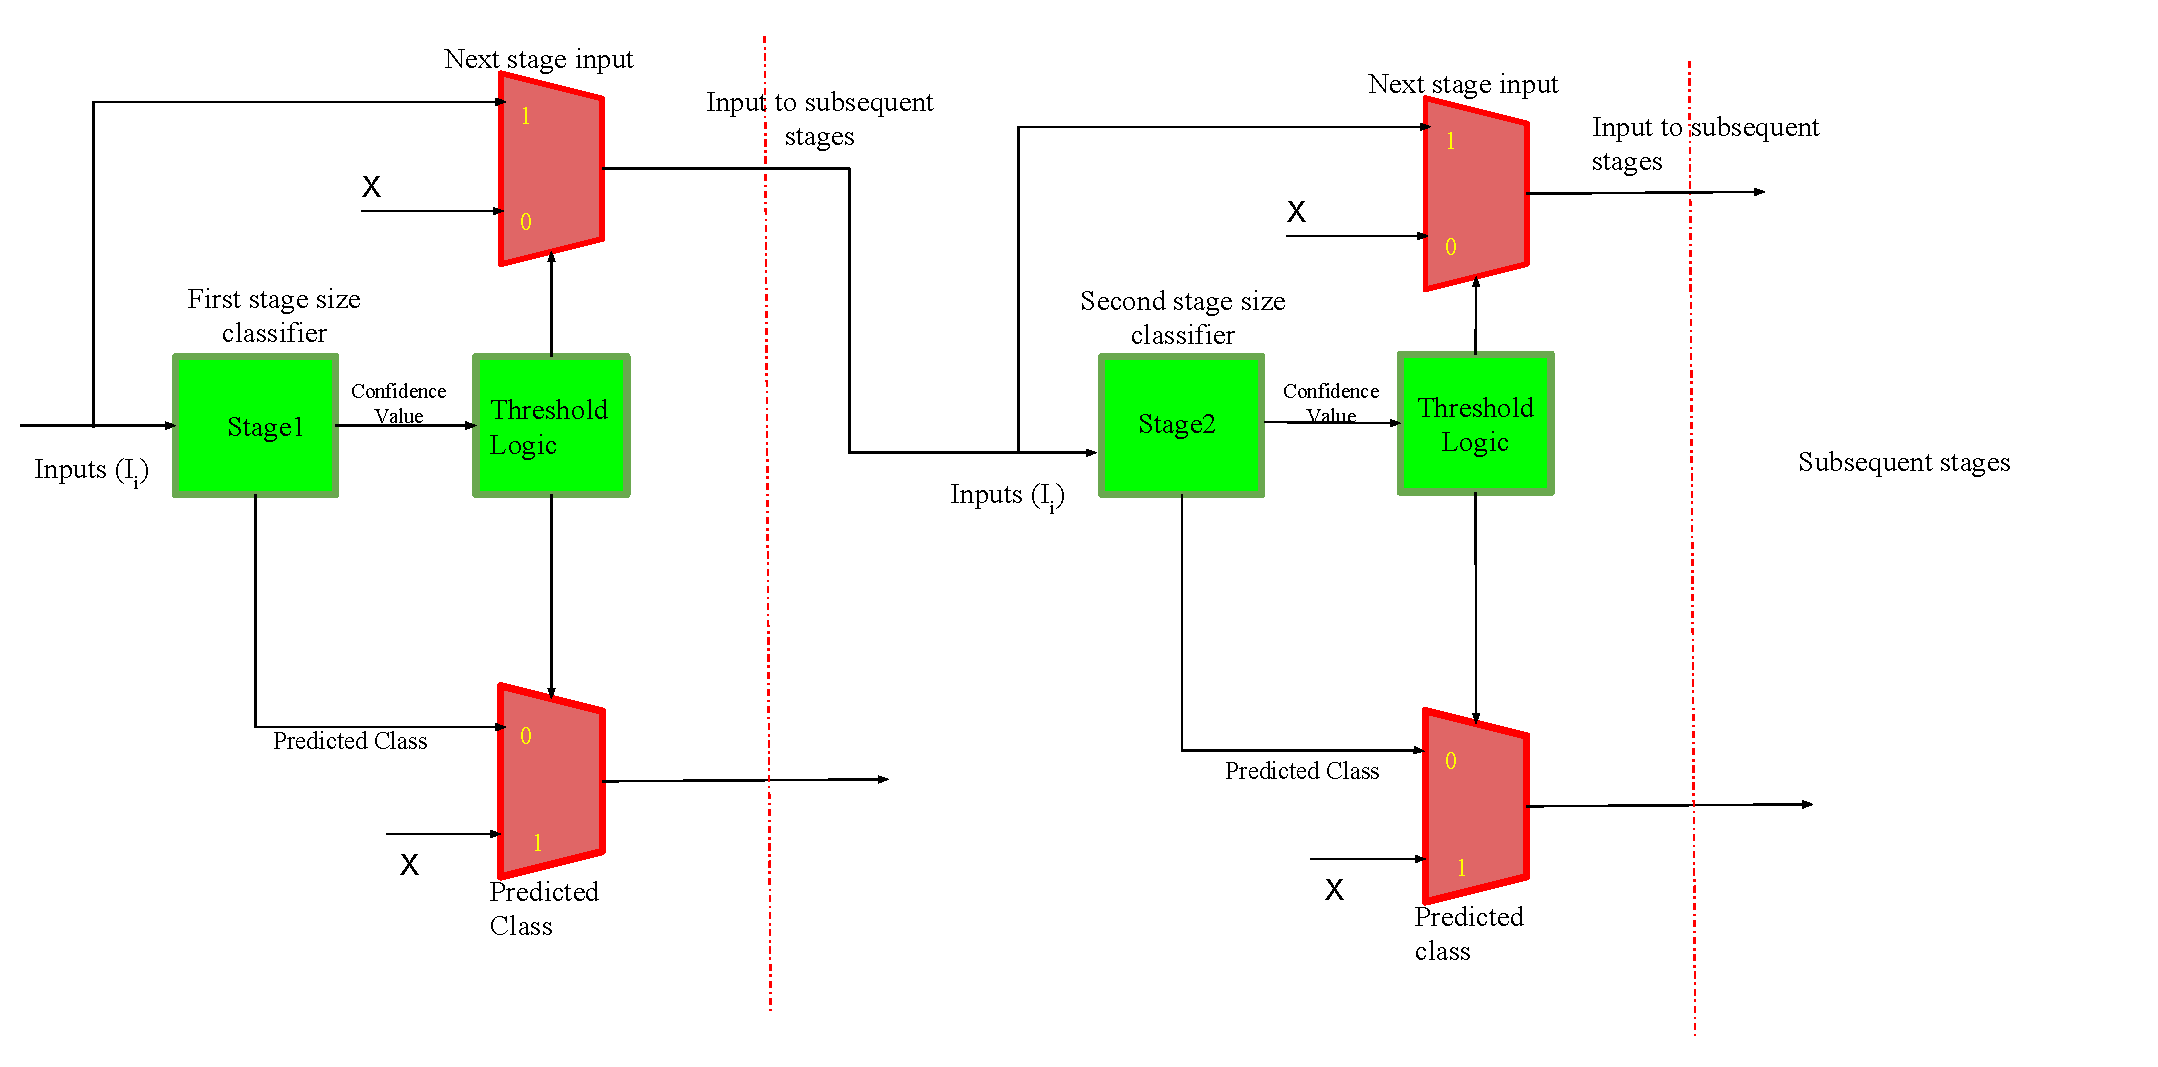
\includegraphics[scale=0.5]{fig/cascaded_size.pdf}
% \caption{Hierarchical SVM $size$ classifier. The first stage $size$ classifier classifies the points as $size = 0$ or $size > 0$ using the thresholding function. The second stage classifier takes the points labelled as $size > 0$ as inputs and uses the thresholding function to classify them as $size = 1$ and $size > 1$. The subsequent \emph{i} stages attempt to classify the input as $size=\emph{i}$ and $size > \emph{i}$.}
% \label{fig:sizesvm}
% \end{center}
% \end{figure}
    \item\textbf{ Boosting the weights of the minority classes}: While the cascaded setup solves the class imbalance problem in the $V_t$ classification, it does not completely resolve the problem in ${size}$ classification. This is because the number of sample points available for the larger sizes is extremely small as can be seen in Table~\ref{tab:dist}. It can be observed from the table that the number of sample points available for $size \geq 2$ is less than $1\%$ which is insufficient for training. This problem is resolved by boosting the weights of the features that belong to the minority classes. During training we manually increase the weights associated with the minority class to improve the performance of each classifier. 
    
  
\end{itemize}



% Please add the following required packages to your document preamble:
% \usepackage{multirow}





% \begin{table}[!t]
% \parbox{.45\linewidth}{

%    \centering

% \begin{tabular}{cc}
% \hline
% $\mathbf{V_t}$ & \textbf{\begin{tabular}[c]{@{}c@{}}Percentage \\  of gates\end{tabular}} \\ \hline \hline
% 0             & 8.47                                                                     \\ \hline
% 1             & 1.86                                                                     \\ \hline
% 2             & 89.67                                                                    \\ \hline
% \end{tabular}
%  \caption{This table shows the number of cells for each $V_t$ in the training dataset. We number the $V_t$ choices and the $size$ choices. A $V_t$ value of 0 indicates that the cell is an $LV_t$ cell while a $V_t$ value of 2 indicates that it is an $HV_t$ cell.}\label{tab:Vt}
   
% %\end{table}
% }
% \hfill
% \parbox{.45\linewidth}{
% %\begin{table}[!t]
%     \centering
%     \begin{tabular}{|c|c|}
%     \hline
%         $size$ & percentage of cells \\ \hline
%         0 & 84.40\\ \hline
%         1 & 13.75\\ \hline
%         2 & 0.7\\ \hline
%         3 & 0.7\\ \hline
%         4 & 0.2\\ \hline
%         $\geq 5$ & 0.25 \\ \hline
        
%         \end{tabular}
%     \caption{This table shows the number of cells for each $size$ in the training dataset. A cell with a $size$ value of 0 indicates that it has the smallest size possible while a cell with a $size$ value of 9 indicates that it has the largest size possible in the standard cell library.}
%     \label{tab:size}
% }
% \end{table}


% \begin{algorithm}[ht]
% %\algsetup{linenosize=\tiny}
%  \LinesNumbered`' 
% %\linesnumbered
% \title{Gateid algorithm}
% \caption{The algorithm that initializes all cells with its respective gateid}
% \label{gateid-algo}
% \KwIn{Netlist of the given circuit C containing N gates represented as a Directed Acyclic Graph (DAG) with each gate initialized to a unique prime number\footnote{The product of prime numbers is always unique and this product can be used to identify recurring sub-circuit patterns} based on gate type. }

% \For {each gate $g$ in $C$}{
%    initialize $gateid.g$ with the prime number corresponding to the gate type of g\;
%    }
%  \For {each gate $g$ in $C$}{  
%    \For{each gate $i$ in $fanins(g)$}{
%         $gateid.g = gateid.g \times gateid.i$\;
        
%         }
        
%    \For{each gate $i$ in $fanouts(g)$}{
%        $ gateid.g = gateid.g \times gateid.i$\;
        
%         }
%     }
% \KwResult{gateid is assigned to each gate}
% \end{algorithm}


%Talking points: No. of datapoints, configuration of the classifier, feature selection, 




%~\ref{learnalgo}. The algorithm has two stages \- lines ~\ref{alg:svmbegin} to ~\ref{alg:svmend} generate a good initial configuration for the netlist by using two hierarchical SVM classifiers one for $V_t$ and one for $size$. lines ~\ref{alg:delay} and lines ~\ref{alg:power} perform delay and power recovery to obtain  a leakage and power optimal configuration. 


\begin{table}[!t]
 \begin{minipage}{0.45\textwidth}
 \caption{The 2-bit prediction-based window sizing strategy adopted by {\it MLTimer}. \textsuperscript{*} The window size is incremented by a constant factor, denoted using $\alpha$.}
 \label{tab:window-sizing-strategy}

 %\begin{center}
 \centering

 %\scalebox{0.9}{

 \begin{tabular}{|c|c|c|p{4cm}|c|}
 \hline
 State & $v_{i-1}$ &$v_i$ &Description &$r(i+1)$ \\
 \hline
 $S_{00}$ &0 &0 &Timing violation in the last two iterations& $1$ \\
 \hline
 $S_{01}$ &0 &1 &Timing violation in $(i-1)^{th}$ iteration and no timing violation in $i^{th}$ iteration& $(r(i))*2$ \\
 \hline
 $S_{10}$ &1 &0 &No timing violation in $(i-1)^{th}$ iteration and timing violation in $i^{th}$ iteration& $r(i) + \alpha$ \textsuperscript{*} \\
 \hline
 $S_{11}$ &1 &1 &No timing violation in the last two iterations& $r(i)^2$ \\
 %\scalebox{0.9}{

 \hline

 \end{tabular}%}
 %\end{center}
 \end{minipage}\hfill
%\begin{figure}[!ht]
\begin{minipage}{0.35\textwidth}
 \begin{center}
 \includegraphics[scale=0.4]{Chapter3/fig/state_machine_window_sizing}
 \captionof{figure}{Transition diagram for the 2-bit prediction scheme adopted by {\it MLTimer}}
 \label{fig:state-machine-window-sizing}
 \end{center}
\end{minipage}
\end{table}


\begin{algorithm}
%\algsetup{linenosize=\tiny}
  \scriptsize
\LinesNumbered
\title{Delay Recovery Algorithm}
\caption{Delay Recovery Algorithm }
\label{alg:delay}
\KwIn{1. Netlist of the given circuit C containing N gates represented as a Directed Acyclic Graph (DAG),2. $V_t$ and $size$ values predicted by the Learning module,3. the multi-$V_t$ standard cell library and 4. the target frequency $F$.}
    \KwOut{Netlist running at the target frequency $F$.}
 $r = r_{init}$\; 
  $state\leftarrow S_{11}$\;
 $N \leftarrow gate\ count$\; 
    Initialize all the gates in $C$ with the corresponding $V_t$ and $size$ values predicted by the SVM engine. If the learning module is not able to predict a $V_t$/$size$ for a gate initialize them to a power optimal configuration $(V_t=2/size=0)$\; 
  Run STA and compute slack for each gate\; 
    \textit{cost function } $=\frac{\delta delay \times slack}{\delta leakage \times \# paths} $\; 
    For each $g_{j}$ ($1 \le j \le N$),\\ \ \ \ \  compute the cost of decreasing the $V_t$, increasing the $size$, and both\; 

 %cost of replacement \leftarrow $\frac{ $ \delta leakage \times slack$ }{$\delta delay \times paths$}$ \;
 A $\leftarrow$ list of replacements sorted in increasing order of \textit{cost function}\;  
%  \tcc{Note that all gates have slack value $\ge$ 0} 
  \While{A not empty}  {
    Take the top $r$ replacements ($A_{1}, A_{2} \ldots A_{r}$) in $A$ \; 
%  \tcc{Local validation}
     For each $A_{j}$ ($1 \le j \le r$),\\ \ \ \ \ Replace $A_{j}$ with its next high performance version (decrease $V_t$ or increase $size$) if $A_{j}$ has positive slack\; 
%  \tcc{Global validation}
      Perform a full STA on C\; 
      \If{ delay violation} {undo all the replacements done in step 12\;
    If $r \leftarrow 1$ mark $A_{j}$ as critical and delete it from A\;
      Update the state as per Figure~\ref{fig:state-machine-window-sizing}\; 
      Update the value of $r$ as per Table~\ref{tab:window-sizing-strategy}, for the new value of state\; 
    }

      \Else {
        Compute the new cost for the committed gates\;

      Update the state as per Figure~\ref{fig:state-machine-window-sizing}\; 
      Update the value of $r$ as per Table~\ref{tab:window-sizing-strategy}, for the new value of state\; 
  }
    }
\end{algorithm}




%write delay and leakage recovery module.
 
\subsection{Delay Recovery Module}
The performance of the learning module is highly dependent on the number and distribution of examples provided during the training phase. An SVM engine might under perform because of improperly chosen features, class imbalance in the dataset or less number of training examples. One or more of the above factors could lead to false positives and false negatives. These false positives and false negatives could lead to delay violations. We use Algorithm~\ref{alg:delay} to fix the timing violations in the circuit.
As seen in Figure~\ref{fig:algo}, Algorithm~\ref{alg:delay} fixes all the delay violation to ensure that the performance of the given circuit $C$ meets the target frequency. Algorithm~\ref{alg:delay} fits into the template of the iterative greedy algorithm described in Algorithm~\ref{alg:naive} except that multiple gates are replaced in each iteration of the algorithm (line 7 of algorithm~\ref{alg:naive} versus line 11 of algorithm~\ref{alg:delay}). The cost function in line 6 of algorithm~\ref{alg:delay} employed is the same as that in~\cite{hu:12}.

Algorithm~\ref{alg:delay} describes the functionality of the delay recovery module. The algorithm adaptively varies $r$ across each timing update. The value of $r$ is varied within a range $[r_{low}, r_{high}]$.In this algorithm, we initialize $r$ to $r_{low}$ and increment the same after each timing update depending on the $state$ of the timing update, until $r$ reaches $r_{high}$. After $r$ reaches $r_{high}$, it is not incremented further. In the experiments reported in this paper, the value of $r_{high}$ is fixed at $\frac{N}{2}$ ($N$ is the number of gates) based on the profiling done to find the effect of varying $r$ on the algorithm run-time for various benchmarks. Let $r(i)$ denote the value of $r$ in iteration $i$. The state transition diagram shown in Figure~\ref{fig:state-machine-window-sizing} in conjunction with Table~\ref{tab:window-sizing-strategy} describe how the value of $r$ is changed across iterations. The states in Figure~\ref{fig:state-machine-window-sizing} are defined in Table~\ref{tab:window-sizing-strategy}. Let $v(i)$ be set to $1$ if there is no timing violation in iteration $i$ else it is set to $0$. Thus the state machine will be at $S_{v_{i-1},v_i}$ at the end of iteration $i$. For example, if there was a timing violation in both iterations $i-1$ and $i$, the state machine will be in $S_{00}$ at the end of iteration $i$. Table~\ref{tab:window-sizing-strategy} describes the change in the value of $r$ in iteration $i+1$, $(r(i+1))$; that depends on the state in iteration $i$. For example, if the state at iteration $i$ is $S_{10}$, then the value of $r(i)$ is incremented by a small factor $\alpha$ in the next iteration $(r(i+1)=r(i)+\alpha)$. 
 
% The state transition We describe the way $r$ varies using the state transition diagram shown in Figure~\ref{fig:state-machine-window-sizing} and the value of $r$ at the end of every timing update is given in Table~\ref{tab:window-sizing-strategy}. It can observed from this transition diagram that $state$ in timing update $i$ can be represented as $S_{v_{i-1},v_i}$, where $v_{i-1}$ and $v_{i}$ are binary digits that denote the status of $(i-1)^{th}$ and $i^{th}$ timing updates respectively. Here, a status ($v$) of $0$ denotes the occurrence of a timing violation while a $1$ denotes a successful timing update.
 
From our experiments, we observe that the iterative correlation was very high for the first few timing updates. This implies that maximum number of gates should get replaced during those timing updates, and hence the initial state is set to $S_{11}$, which quadratically scales the window size in successive timing updates. The value of $r_{low}$ is set to $2$. A successful timing update at the end of the first iteration would cause the state to remain at $S_{11}$ while increasing $r$ quadratically to $4$, and a timing violation would cause the state to change to $S_{10}$, causing $r$ to be incremented by a small positive constant $\alpha$. A timing violation in the second update would set the state to $S_{00}$ and the window to $1$. This explains the adaptive window sizing procedure. As shown in Figure~\ref{fig:ropt} replacing $r_{opt}$ number of gates gives the best speed-up possible. However, $r_{opt}$ varies across each timing update. Ideally replacing $r_{opt,i}$\footnote{$r_{opt,i}$ is the optimal window size for the $i^{th}$ update.} gates for each of the $i$ timing updates will result in the best possible speedup. However, the value of $r_{opt,i}$ cannot be precomputed. From our initial experiments we observed that $r_{i+1}$ is strongly related to the outcome of the previous timing updates. By taking into account the outcome of the last $k$-timing updates, the likelihood of obtaining the $r_{opt}$ for the next timing update is maximized. In our setup we use a 2-bit state based sizing scheme. 
\noindent We observed that there is no significant improvement for large values of $k$. This is because the algorithm takes a large amount of time to recover from a suboptimal window size or to get to the optimal window size for a given iteration. We define this phenomenon as inertia. Consider the following scenario. If the current window size is $r_{high}$ and there is a timing violation. The number of iterations required to identify the gate causing the timing violation is $2$. However, for a large value of $k$ this increases thereby causing the algorithm to spend significant amount of time on useless timing updates. 


%\noindent We use Algorithm~\ref{alg:delay} to fix the delay violations in the circuit. We initialize the gates in netlist with $V_t$ and $size$ values predicted by the classifiers. We run an initial STA and identify the target gates using the same cost function defined in ~\cite{hu:12}.  Recovering the delay of gate $g_{i}$ will impact the other gates in the fanin/fanout cone of $g_i$. The chosen cost function computes the impact of a change in the $V_t$ or $size$ of a gate on its neighbours by computing the change in slack across all the gates in the fanin and fanout cone of $g_i$ denoted using the term $\delta delay$ in the cost function. A gate with large number of fanins/fanouts might have significantly high $\delta delay$, hence we also take into account the number of negative slack paths passing through the gate $g_i$ using the term $\#paths$. The term $\delta leakage$, which accounts for the change in leakage due to the replacement, prohibits the gate from trading off significantly large amount of power in order to improve performance.

Each execution of the \textbf{while} loop corresponds to one update interval. During each  update interval we do the following:
\begin{itemize}
\item We compute the cost of decreasing the $V_t$, increasing the $size$ and both for every gate and add them to a list \textit{A}.
\item The first $r$ choices in the decreasing order of their cost are replaced.
\item We then check for any timing violations by running a full STA. We do not use an incremental STA because running timing analysis for each gate in the window, would impose significant runtime penalty for large window sizes, ultimately offsetting the speed-up obtained by postponing the timing analysis.
\item If there is a delay violation, undo all the replacements 
\begin{itemize}
\item if $r$ is $1$, then mark the corresponding gate as critical so that it cannot participate in any further timing optimizations.
\item Update $state$ and compute new value of $r$.
\end{itemize}
\item If the timing evaluation is successful
\begin{itemize}
    \item Compute the new costs for the gates that got committed. If the gates cannot participate in further updates (gates have reached lowest $V_t$ or $size$) mark them as critical and remove them from A.
\item Update $state$ and compute the new value of $r$.
\item if value of $r$ is greater than A, then we resize $r$ to $\frac{A.size}{2}$.
\end{itemize}

\end{itemize}

\begin{algorithm}[!t]
%\algsetup{linenosize=\tiny}
  \scriptsize
 \LinesNumbered
 \title{The {\it Leakage Power recovery } algorithm}
 \caption{The Leakage Power recovery algorithm}
 \label{exponential-algo}
\KwIn{1. Netlist of the given circuit C represented as a Directed Acyclic Graph (DAG) running at target frequency $F$,2. initial window size ($r_{low}$) and upper bound on window size ($r_{high}$) and 3. a multi-$V_t$ standard cell library.}
\KwOut{The leakage optimized netlist running at target frequency $F$.} 
  $r = r_{low}$\; 
  $state\leftarrow S_{11}$\;
 $N \leftarrow gate\ count$\;
  Run STA and compute slack for each gate\;
    \textit{cost function} $=slack$\;
 A $\leftarrow$ list of gates with non-zero slacks, sorted in descending order of \textit{cost function}\; 
%  \tcc{Note that all gates have slack value $\ge$ 0} 
  \While{A not empty}  {
    Take the top $r$ gates ($g_{k_1}, g_{k_2} \ldots g_{k_r}$) in $A$ \;
%  \tcc{Local validation}
     For each $g_{k_j}$ ($1 \le j \le r$), replace the gate with its next power optimal version  (increase $V_t$ or decrease $size$) if gate $g_{k_j}$ has sufficient positive slack\;
%  \tcc{Global validation}
      Perform a full STA on C\;
      \If {delay violation} {
          Undo all the replacements done in step 9\;
          If $r\leftarrow1$ mark $A_{j}$ as critical and delete it from A\;
            Update the state as per Figure~\ref{fig:state-machine-window-sizing}\;
      Update the value of $r$ as per Table~\ref{tab:window-sizing-strategy}, for the new value of state\;

      }
      \Else{
          Compute the new cost for the committed gates\;
      Update the state as per Figure~\ref{fig:state-machine-window-sizing}\;
      Update the value of $r$ as per Table~\ref{tab:window-sizing-strategy}, for the new value of state\;
  }
    }
 \end{algorithm}




\subsection {Leakage Power Recovery Module}
The delay recovery module ensures that there are no timing violations in the netlist. An iterative algorithm described in Algorithm~\ref{exponential-algo} is employed to recover the leakage power from the netlist. We initialize the window size $r_{low}$ and $state$ to $S_{11}$.  We perform an initial timing analysis to identify the target gates and follow the steps similar to Algorithm~\ref{alg:delay} to perform multiple gate replacements in order to minimize the leakage power. The leakage recovery algorithm uses \textit{slack} as the cost function to identify gates for replacement in each iteration. In the leakage recovery step, the amount of slack indicates the conduciveness of the gate for replacement.  A gate with a high positive slack  can be replaced without having to worry about the impact on the neighbourhood gates while gates with negative slack or zero slack cannot be chosen for power optimization.  In our algorithm only the gates with positive slack are considered during each iteration.

During each iteration, the gates are sorted in the descending order of slack. The top $r$ gates are selected and replaced with their next slower version provided they have sufficient slack. We then check for timing violations by running a full STA. Though we consider only gates with positive slack, there might be timing violations because two gates in the same path could have positive slack and hence would be chosen for update. However, simultaneous updates on both the gates could result in a timing violation. In case of a delay violation we undo the replacements and update the state variable and $r$. If there is no timing violation we compute the new slack values for all the gates and update the state variable and $r$.


 
 


 



\section{Related Work}
%\label{sec:related}
\label{sec:related-work}
\noindent The TC-DSP problem being NP-complete~\cite{feng:09}, brute force search cannot find an optimal solution. Several heuristics have been proposed in the past to address this problem~\cite{feng:09,wu:08,fishburn:85,sundarajan:99,liu:10,hu:12, mok:12,coudert:97}. 
In~\cite{fishburn:85} it was shown that the continuous sizing problem 
with area minimization objective is convex, and a greedy sensitivity-based 
heuristic was proposed to solve the same. Similarly, in~\cite{sundarajan:99}, 
a continuous optimization is performed, following which the solutions are 
discretized. However, this type of discretization is known to produce 
suboptimal solutions due to significant round-off errors. In~\cite{feng:09}, 
a polynomial time approximation scheme was proposed, but this scheme does not 
scale well for circuits with large number of gates as the run time runs into minutes even for circuits with less than 5000 gates. Another analytical algorithm was provided for the same 
in~\cite{liu:10}, but this algorithm also takes several minutes even for 
circuits whose gate-count is less than 20,000. Nothing is mentioned in~\cite{liu:10} about the scalability of the running time of the algorithm with respect to large circuits. In~\cite{mok:12}, a survey 
of all the existing algorithms for the sizing problem is provided and is concluded 
that {\em no algorithm exists that consistently provides good results for all circuits}. The ISPD 2012~\cite{ispdcontest1} and ISPD 2013~\cite{ispdcontest2} contests provided a set of benchmark circuits that were targeted at evaluating the quality of any sizing technique. 
However, it was shown in both~\cite{hu:12} and~\cite{mok:12} that iterative 
greedy heuristics are fastest and most effective in solving the TC-DSP. 

The TC-DSP is presented as an instance of Lagrangian Relaxation (LR) problem in~\cite{Hu:11}. The objective is to minimize leakage and the algorithm places a penalty for any delay violations. The timing constraints are introduced in the LR formulation.  The netlist is modeled as a directed acyclic graph and the discrete gate version characteristics are based
on timing tables provided by the gate library. A Dynamic Programming algorithm
based on critical tree extraction is proposed to solve the LR optimization problem for discrete gates. An accurate timer is used for sign-off and slack computation.
 
%~\cite{li:12}, ~\cite{livramento:13}, ~\cite{hu:12} and ~\cite{flach:13} use the ISPD2012 framework. 
 Empirically it is observed in this paper that some commercial synthesis tools consume less time for the design optimization time but the solution quality is far from desirable. To avoid compromise on the solution quality, there are a few heuristics like those proposed in \cite{wu:08} and \cite{hu:12}, which focus on employing parallel and concurrent techniques to reduce the run-time of the optimizer. The speed-up achieved through this parallelization is not significant though the effort involved in parallelizing the code could be significant. A common scalable solution to the TC-DSP problem is to iteratively replace gates with their different  versions and perform a static timing analysis (STA) at the end of every iteration to check for timing violations due to the gate replacements.
 As the optimization process proceeds, the algorithm experiences high rejection rates, making the performance of the STA 
engine very crucial for scalability~\cite{papa:10}. Next, we describe the existing STA techniques reported
in literature. 
%
Initial Static Timing Analysis (STA) engines always processed an entire design, which is impractically expensive for evaluating every 
replacement~\cite{papa:10}. It is to be noted that replacing the $V_t$/gate-size of a gate $g_i$, changes the arrival times of gates only in the fan-in and fan-out cones\footnote{Fan-in/Fan-out cone of a gate $g$ is defined as the sub-circuit that drives/is driven by the gate $g$.} of $g_i$, while the arrival times of other gates remain unaffected. By performing STA for the entire design, we may end up computing known values repeatedly. 
To improve the efficiency of the STA engine, several {\em incremental} STA techniques have been proposed in the past~\cite{lee:95,abato:96,sapatnekar:96,mondal:04,das:06,papa:08}. In~\cite{lee:95}, {\em incremental} STA is performed by solving 
the {\em incremental longest path problem}, with a novel algorithm which is linear in the number of edges in the {\em dominance fan-out cone}. In~\cite{abato:96}, a frontier is established by recording the leftmost and rightmost gates in the fan-in and fan-out cone of each gate that get affected by the change in relative timing values are recorded.
Based on a request, incremental timing analysis is performed on the modified design
employing the recorded frontiers of change to limit the timing analysis to 
the {\em affected} regions of the circuit alone. An input based path sensitization approach 
was used for incremental STA in~\cite{sapatnekar:96}.
On a similar note, in~\cite{coudert:97}, the incremental timer is accelerated by only updating a 
set of gates that are in the neighborhood of the gate whose timing value has been updated. 
In~\cite{mondal:04}, timing queries were modeled using temporal logic and an efficient 
algorithm was proposed to answer those queries. Similarly, in~\cite{das:06}, a more 
efficient incremental STA algorithm which exploits the circuit structure was proposed. 
In all these works, path based algorithms were proposed to 
increase the performance of incremental STA, but none of them except~\cite{abato:96} looked 
at reducing the number of times the incremental STA needs to be performed. 
Even in~\cite{abato:96}, although incremental STA is not performed in every iteration, 
nonetheless some computation is performed in every iteration relating to the signal propagation. 
As a result, the running time complexity does not decrease significantly compared to the use of a normal STA. 
For e.g., in~\cite{hu:12}, in spite of using a state-of-art incremental timer, the optimization 
took greater than 20 hours. It can be seen from the above works that the STA engines reported so far consume a significant time. The number of times the STA needs to be performed (timing updates) grows linearly with the size of the circuit. Reducing the number of times such updates are performed results in a reduction in the overall running time of the algorithm. This reduction without compromising on the solution quality is the challenge that forms one of the central themes of this paper.


%
%This paper uses the {\em lazy timing evaluation} to arrive at a fast algorithm for the TC-DVSP. 
%The {\em laziness} is to avoid performing the STA after every iteration but to perform the same 
%once in several iterations. To sum up, the main contributions of the work are as follows:
%\begin{enumerate}
%\item We observe that iterative {\em slack-based} greedy discrete $V_t$ sizing exhibits %significant 
%speed-up while retaining/improving the solution quality over iterative  {\em sensitivity-based} 
%greedy discrete  sizing~\cite{hu:12,chinnery:05}. 
%\item We show that in iterative slack-based discrete $V_t$ sizing, there is a significant correlation 
%between the ordering of gates based on slack in the current iteration and the ordering of gates that 
%are replaced in successive iterations.
%\item Exploiting this high correlation, this paper proposes a {\em lazy timing analysis} coupled with an {\em Adaptive Window sizing (AWS) scheme for decision making} to perform {\em multiple $V_t$ replacements} between successive timing updates, thereby producing solutions that are at least {\em an order of magnitude} faster and consume lesser leakage power, 
%when compared to an existing commercial multi-$V_t$ synthesis tool.
%\end{enumerate}
{\em Lazy evaluation} is a popular paradigm in improving the computational efficiency of iterative algorithms.
The line sweep algorithm used in the VLSI routing checkers is based on this technique.
In \cite{papa:10}, it was shown that lazy STA when employed for {\em timing optimization} can result in more
than 2$\times$ speed-up, when combined with transactional timing analysis.
{\em It should be noted that lazy updates may not be acceptable for all optimization problems}. 
An {\em optimistic} approach with {\em lazy timing updates},
may lead to unnoticed timing violations that might have occurred on the gates
that have been marked for timing updates. This demands backtracking that actually ends up
increasing the running time of the algorithm, defeating the whole purpose. 
Interestingly, {\em lazy updates} combined with an efficient backtracking procedure can speed 
up the iterative algorithms that solve the {\em timing optimization} problem.



%The leakage power minimization problem has been studied over the last 30 years and there has been a considerable amount of work done in this regard. The work can be primarily divided into two classes: heuristic based approach and analytical approach. 
%Since the leakage power minimization problem is NP-Hard, heuristic based approaches have focussed on  effective search space exploration. Works like %inser references here 
%have focussed on developing metrics that help in identifying the right candidate cells and works like % insert references
%have focussed on novel search space exploration heuristics. However the growing circuit complexity has necessitated the need for  robust heuristics which can both handle placement-aware, routing-aware solutions and the need for faster turn around times has necessitated the need for faster solutions. This is highlighted by the ISPD2012 contest which had weightage for runtime constraints. This has motivated researchers to develop runtime aware heuristics. %insert references 
%have adopted a multi-threaded approach to reduce the run-time overheads. 
%Initial analytical methods focussed on posing the leakage optimization problem as a continous sizing problem. However the degradation in solution qualty incurred due to converting the final solution into a discrete value led researchers to pose the leakage optimization problem as a discrete sizing problem. Recent works like %insert references here
%have focussed on modelling the leakage opitmization problem as a  lagrangian relaxation problem. %insert refeerences 
%have also used multi threading to speed up the optimization process.

%Initial Static Timing Analysis (STA) engines always processed an entire design, 
%which is impractically expensive for evaluating every $V_t$ 
%replacement~\cite{papa:10}. It is to be noted that replacing $V_t$ of a 
%gate $g_i$, changes the arrival times of gates only in the fan-in and 
%fan-out cones of $g_i$, while the arrival times of other gates remain unaffected. By performing STA for the entire design, we may end up computing known values repeatedly. 
%To improve the efficiency of the STA engine, several {\em incremental} STA techniques 
%have been proposed in the past~\cite{lee:95,abato:96,sapatnekar:96,mondal:04,das:06,papa:08}.
%In~\cite{lee:95}, {\em incremental} STA is performed by solving 
%the {\em incremental longest path problem}, with a novel algorithm which is linear in 
%the number of edges in the {\em dominance fan-out cone}. In~\cite{abato:96}, the leftmost 
%and rightmost frontiers of change in relative timing values are %recorded.
%Based on a request, incremental timing analysis is performed on the modified design
%employing the recorded frontiers of change to limit the timing analysis to 
%the {\em affected} regions of the circuit alone. An input based path sensitization approach 
%was used for incremental STA in~\cite{sapatnekar:96}.
%On a similar note, in~\cite{coudert:97}, the incremental timer is accelerated by only updating a 
%neighborhood set of gates. 
%In~\cite{mondal:04}, timing queries were modeled using temporal logic and an efficient 
%algorithm was proposed to answer those queries. Similarly, in~\cite{das:06}, a more 
%efficient incremental STA algorithm which exploits the circuit structure was proposed. 
%In all these works, path based algorithms were proposed to 
%increase the performance of incremental STA, but none of them except~\cite{abato:96} looked 
%at reducing the number of times the incremental STA needs to be performed. 
%Even in~\cite{abato:96}, although incremental STA is not performed in every iteration, 
%nonetheless some computation is performed in every iteration relating to the signal propagation. 
%As a result, the running time complexity does not decrease significantly. 
%For e.g., in~\cite{hu:12}, in spite of using a state-of-art incremental timer, the optimization 
%took $>20$ hours. It can be seen from the above works that the STA engines reported so far consume a significant time. The number of times the STA needs to be performed (timing updates) grows linearly with the size of the circuit. Reducing the number of times such updates are performed results in a reduction in the overall running time of the algorithm. This observation forms the central theme of this paper.

%~\cite{hu:12} ~\cite{mustafa:11} ~\cite{chinnery:05} ~\cite{li:93} ~\cite{dennard:74} ~\cite{borkar:99} ~\cite{baauw:03} ~\cite{hu:09} ~\cite{davoodi:08} ~\cite{boyd:08} ~\cite{flach:14} ~\cite{parhi:99} ~\cite{papa:10} ~\cite{lee:95} ~\cite{sapatnekar:96} ~\cite{papa:08} ~\cite{hu:10}
%~\cite{coudert:97} ~\cite{kahng:16} ~\cite{ketkar:00} ~\cite{Han:2014} ~\cite{Kahng:13} ~\cite{kang:13} ~\cite{chu:15} ~\cite{sharma:15} ~\cite{6513816} ~\cite{reimann:2016} ~\cite{li:2012} ~\cite{Davoodi}


%include ISPD 2012, 2013 opentimer references.
\section{Results}
\label{sec:results}
% \begin{table}[!ht]
% \centering
% \caption{My caption}
% \label{my-label}
% \begin{tabular}{|p{1.2cm}|l|l|l|l|l|l|}
% \hline
% \multirow{2}{*}{\begin{tabular}[c]{@{}c@{}}Feature \\ Name\end{tabular}} & \multicolumn{2}{c}{Vt Classifier}                                       & \multicolumn{4}{|c|}{Size classifier}                                                                                                   \\ \cline{2-7} 
%                                                                          & \multicolumn{1}{c|}{1} & \multicolumn{1}{c|}{2} & \multicolumn{1}{c|}{ 1} & \multicolumn{1}{c|}{ 2} & \multicolumn{1}{c|}{3} & \multicolumn{1}{c|}{4} \\ \hline
% Sub-circuit                                                              & \multicolumn{1}{l|}{}        &                               &                               &                               &                              &                              \\ \hline
% Gate Type                                                                & \multicolumn{1}{l|}{}        &                               &                               &                               &                              &                              \\ \hline
% LNS                                                  & \multicolumn{1}{l|}{}        &                               &                               &                               &                              &                              \\ \hline
% \#Fanins                                                                 & \multicolumn{1}{l|}{}        &                               &                               &                               &                              &                              \\ \hline
% \#Fanouts                                                                & \multicolumn{1}{l|}{}        &                               &                               &                               &                              &                              \\ \hline
% \begin{tabular}[c]{@{}l@{}}\#Negative \\ Slack Paths\end{tabular}                                          & \multicolumn{1}{l|}{}        &                               &                               &                               &                              &                              \\ \hline
% Slack                                                                    & \multicolumn{1}{l|}{}        &                               &                               &                               &                              &                              \\ \hline
% \end{tabular}
% \end{table}
% \begin{table*}[!ht]
% \centering
% \caption{result3}
% \label{results3}
% \begin{tabular}{|l|c|l|l|l|l|l|l|l|l|l|l|}
% \hline
% \multicolumn{1}{|c|}{\begin{tabular}[c]{@{}c@{}}Benchmark \\  Name\end{tabular}} & \begin{tabular}[c]{@{}c@{}}Number \\ Of gates\end{tabular} & \multicolumn{1}{c|}{\begin{tabular}[c]{@{}c@{}}Target \\ Delay\end{tabular}} & \begin{tabular}[c]{@{}l@{}}Inital \\ Delay\end{tabular} & \multicolumn{2}{c|}{SVM}                                         & \multicolumn{2}{c|}{Final}                                      & \multicolumn{2}{c|}{Igor Markov}                               & \multicolumn{2}{c|}{Flach}                                     \\ \hline
% \multicolumn{1}{|c|}{}                                                           &                                                            & \multicolumn{1}{c|}{}                                                        & \multicolumn{1}{c|}{}                                   & \multicolumn{1}{c|}{Delay (ns)} & \multicolumn{1}{c|}{Power (W)} & \multicolumn{1}{c|}{Delay (ns)} & \multicolumn{1}{c|}{Power(W)} & \multicolumn{1}{c|}{Delay(ns)} & \multicolumn{1}{c|}{Power(W)} & \multicolumn{1}{c|}{Delay(ns)} & \multicolumn{1}{c|}{Power(W)} \\ \hline
% DMA\_fast                                                                        & 25.3K                                                      &                                                                              &                                                         &                                 &                                &                                 &                               &                                &                                                0.299    &       &                               \\ \hline
% DMA\_slow                                                                        & 25.3K                                                      &                                                                              &                                                         &                                 &                                &                                 &                               &                                &                                                       0.145   &     &                               \\ \hline
% pci\_fast                                                              & 33.2K                                                      &                                                                              &                                                         &                                 &                                &                                 &                               &                                &                                                     0.183     &     &                               \\ \hline
% pci\_slow                                                              & 33.2K                                                      &                                                                              &                                                         &                                 &                                &                                 &                               &                                &                                                  0.111         &    &                               \\ \hline
% des\_perf\_fast                                                                  & 111K                                                       &                                                                              &                                                         &                                 &                                &                                 &                               &                                &                                                         1.842   &   &                               \\ \hline
% des\_perf\_slow                                                                  & 111K                                                       &                                                                              &                                                         &                                 &                                &                                 &                               &                                &                                                          0.614   &  &                               \\ \hline
% vga\_lcd\_fast                                                                   & 165K                                                       &                                                                              &                                                         &                                 &                                &                                 &                               &                                &                                                            0.471  & &                               \\ \hline
% vga\_lcd\_slow                                                                   & 165K                                                       &                                                                              &                                                         &                                 &                                &                                 &                               &                                &                                                            0.351  & &                               \\ \hline
% b19\_fast                                                                        & 219K                                                       &                                                                              &                                                         &                                 &                                &                                 &                               &                                &                                                           0.771   & &                               \\ \hline
% b19\_slow                                                                        & 219K                                                       &                                                                              &                                                         &                                 &                                &                                 &                               &                                &                                                             0.583 & &                               \\ \hline
% leon3mp\_fast                                                                    & 649K                                                       &                                                                              &                                                         &                                 &                                &                                 &                               &                                &                                                             1.487 & &                               \\ \hline
% leon3mp\_slow                                                                    & 649K                                                       &                                                                              &                                                         &                                 &                                &                                 &                               &                                &                                                            1.341  & &                               \\ \hline
% netcard\_fast                                                                    & 959K                                                       &                                                                              &                                                         &                                 &                                &                                 &                               &                                &                                                            1.861  & &                               \\ \hline
% netcard\_slow                                                                    & 959K                                                       &                                                                              &                                                         &                                 &                                &                                 &                               &                                &                                                           1.770  &  &                               \\ \hline
% \end{tabular}
% \end{table*}


% Please add the following required packages to your document preamble:
% \usepackage{multirow}
% Please add the following required packages to your document preamble:
% \usepackage{multirow}
% \begin{table}[]
% \centering
% \caption{My caption}
% \label{my-label}
% \begin{tabular}{|l|l|l|l|l|l|}
% \hline
% \multirow{3}{*}{Benchmark} & \multicolumn{5}{c|}{Runtime}                                                            \\ \cline{2-6} 
%                            & \multirow{2}{*}{Igor Markov} & \multirow{2}{*}{Flach} & \multicolumn{3}{c|}{\textit{MLTimer}} \\ \cline{4-6} 
%                            &                              &                        & SVM  & Delay Recovery  & Total  \\ \hline
% DMA\_fast                  &                              &                        &      &                 &        \\ \hline
% DMA\_slow                  &                              &                        &      &                 &        \\ \hline
% pci\_fast        &                              &                        &      &                 &        \\ \hline
% pci\_brdige32\_slow        &                              &                        &      &                 &        \\ \hline
% vga\_lcd\_fast             &                              &                        &      &                 &        \\ \hline
% vga\_lcd\_slow             &                              &                        &      &                 &        \\ \hline
% des\_perf\_fast            &                              &                        &      &                 &        \\ \hline
% des\_perf\_slow            &                              &                        &      &                 &        \\ \hline
% b19\_fast                  &                              &                        &      &                 &        \\ \hline
% b19\_slow                  &                              &                        &      &                 &        \\ \hline
% leon3mp\_fast              &                              &                        &      &                 &        \\ \hline
% leon3mp\_slow              &                              &                        &      &                 &        \\ \hline
% netcard\_fast              &                              &                        &      &                 &        \\ \hline
% netcard\_slow              &                              &                        &      &                 &        \\ \hline
% \end{tabular}
% \end{table}


% Please add the following required packages to your document preamble:
% \usepackage{multirow}
% Please add the following required packages to your document preamble:
% \usepackage{multirow}
% Please add the following required packages to your document preamble:
% \usepackage{multirow}
\begin{table*}[!t]
\caption{Leakage power and Runtime comparisons between the baseline greedy algorithm and the \textit{MLTimer} algorithm on the ISPD 2012 benchmarks. Implementation 1 is the baseline implementation(non-SVM,non-adaptive timing analysis), Implementation 2 is with SVM and non-adaptive timing analysis, Implementation 3 is with non-SVM and adaptive timing analysis and Implementation 4 is with SVM and adaptive timing analysis. It can be seen that using just SVM improves the solution quality greatly, while using just the adaptive timing analysis improves the runtime. A combination of both improves the runtime and solution qualtiy.}
\label{tab:tab5}

\begin{tabular}{|l|l|l|l|l|l|l|l|l|l|}
\hline
\multirow{2}{*}{Benchmarks} & \multirow{2}{*}{\#Gates} & \multicolumn{2}{l|}{Implementation 1}                                                                                                         & \multicolumn{2}{l|}{Implementation 2}                                                                                                           & \multicolumn{2}{l|}{Implementation 3}                                                                                                        & \multicolumn{2}{l|}{Implementation 4}                                                                                                        \\ \cline{3-10} 
                            &                          & \begin{tabular}[c]{@{}l@{}}Run-\\ time \\ (mins)\end{tabular} & \begin{tabular}[c]{@{}l@{}}Leakage \\ Power\\ (W)\end{tabular} & \begin{tabular}[c]{@{}l@{}}Run-\\ time\\ (mins)\end{tabular} & \begin{tabular}[c]{@{}l@{}}Leakage \\ Power\\ \\ (W)\end{tabular} & \begin{tabular}[c]{@{}l@{}}Run-\\ time\\ (mins)\end{tabular} & \begin{tabular}[c]{@{}l@{}}Leakage\\  Power\\ (W)\end{tabular} & \begin{tabular}[c]{@{}l@{}}Run-\\ time\\ (mins)\end{tabular} & \begin{tabular}[c]{@{}l@{}}Leakage \\ Power\\ (W)\end{tabular} \\ \hline
DMA\_fast                   & 23,000                   & 16                                                            & 0.79                                                           & 14.00                                                        & 0.30                                                              & 14.00                                                        & 0.79                                                           & 13.00                                                        & 0.30                                                           \\ \hline
pci\_bridge32\_fast         & 30,000                   & 37                                                            & 0.25                                                           & 17.00                                                        & 0.14                                                              & 17.00                                                        & 0.24                                                           & 17.00                                                        & 0.14                                                           \\ \hline
des\_perf\_fast             & 102,000                  & 219                                                           & 1.73                                                           & 164.00                                                       & 1.80                                                              & 190.00                                                       & 1.73                                                           & 130.00                                                       & 1.80                                                           \\ \hline
vga\_lcd\_fast              & 148,000                  & 384                                                           & 2.80                                                           & 139.00                                                       & 0.47                                                              & 207.00                                                       & 2.72                                                           & 77.00                                                        & 0.47                                                           \\ \hline
b19\_fast                   & 213,000                  & 547                                                           & 2.13                                                           & 239.00                                                       & 0.75                                                              & 366.00                                                       & 2.13                                                           & 174.00                                                       & 0.75                                                           \\ \hline
leon3mp\_fast               & 540,000                  & 2,046                                                         & 4.00                                                           & 875.00                                                       & 1.49                                                              & 716.00                                                       & 4.00                                                           & 639.00                                                       & 1.49                                                           \\ \hline
netcard\_fast               & 861,000                  & 1,033                                                         & 2.09                                                           & 519.00                                                       & 1.77                                                              & 609.00                                                       & 2.07                                                           & 306.00                                                       & 1.77                                                           \\ \hline
\end{tabular}
\end{table*}

\begin{table*}[!ht]
%\centering
\caption{Leakage power comparisons with ISPD 2012 contest winners and other state of the art works. We use geometric mean to calculate the efficiency of our proposed solution. We exclude the infeasible solutions in our mean calculation. All the solutions reported below have no timing violations.}
\label{tab:tab6}

    \begin{tabular}{|l|l|l|p{1.2cm}|p{1.6cm}|p{1.6cm}|p{1cm}|l|p{1.2cm}|}
\hline
\multirow{2}{*}{Benchmark} & \multirow{2}{*}{\begin{tabular}[c]{@{}l@{}}Number \\ of gates\end{tabular}} & \multicolumn{5}{c|}{Leakage Power (W)} & \multicolumn{2}{c|}{Runtime (mins)}\\ \cline{3-9} 
    &  & \cite{hu:12}  & NTUgs & UFRGSgs & Powervalve & \textbf{Ours} & \cite{hu:12} & \textbf{Ours}\\ \hline
    \texttt{DMA\_fast} & 23,000 & 0.30  & 0.51 & 0.32 & 0.31 & 0.30 & 13.90 & 13.30\\ \hline
    \texttt{DMA\_slow} & 23,000  & 0.15  & 0.21 & 0.16 & 0.15 & 0.14 & 9.90 & 7.51 \\ \hline
    \texttt{pci\_fast} & 30,000 & 0.18  & 0.51 & 0.17 & 0.23 & 0.14 & 13.00 & 17.10
     \\ \hline
    \texttt{pci\_slow} & 30,000 & 0.11   & 0.20 & 0.12 & 0.12 & 0.09 & 10.20 & 9.32 \\ \hline
    \texttt{des\_perf\_fast} & 102,000 & 1.84 & 2.39 & 3.52 & 2.32 & 1.80  & 82.70 & 130.40 \\ \hline
    \texttt{des\_perf\_slow} & 102,000 & 0.61 & 0.67 & 0.88 & 0.70 & 0.64 & 70.10 & 43.50 \\ \hline
    \texttt{vga\_lcd\_fast} & 148,000 & 0.47 & 0.76 & 0.58 & 0.77 & 0.47 & 45.60 & 77.32\\ \hline
    \texttt{vga\_lcd\_slow} & 148,000 & 0.35 & 0.42 & 0.38 & 0.39 & 0.37 & 87.50 & 50.40 \\ \hline
    \texttt{b19\_fast} & 213,000 & 0.77 & 2.71 & - & 4.49 & 0.75 & 206.50 & 174.11 \\ \hline
    \texttt{b19\_slow} & 213,000 & 0.58 & 0.63 & 0.61 & 0.74 & 0.61 & 213.90 & 102.20\\ \hline
    \texttt{leon3mp\_fast} & 540,000 & 1.49 & -&  - & 4.94 & 1.49 & 1,323.20 & 639.40\\ \hline
    \texttt{leon3mp\_slow} & 540,000 & 1.34 & 1.42 & 1.79 & 2.96 & 1.30 & 1,274.20 & 325.13  \\ \hline
    \texttt{netcard\_fast} & 861,000 & 1.86 & 2.01 & 2.30 & 2.97 & 1.86 & 1,096.90 & 306.57\\ \hline
    \texttt{netcard\_slow} & 861,000 & 1.77 & 1.77 & 1.97 & 1.94 & 1.77 & 299.90 & 164.14\\ \hline
Geometric mean &  & $1.03\times$ & $1.52\times$ & $1.13\times$ & $1.57\times$ &   & $1.44\times$ & \\ \hline
\end{tabular}
\end{table*}

% Please add the following required packages to your document preamble:
% \usepackage{multirow}
\begin{table*}[!ht]
\centering
\caption{Leakage power comparisons with \cite{hu:13} on the  ISPD 2013 contest benchmark. All the solutions reported below are violation free. It can be observed that \texttt{MLTimer} outperforms \cite{hu:13} both with respect to leakage power and runtime on the larger benchmarks. The detailed results for other benchmarks were not reported in \cite{hu:13}.}
\label{tab:tab34}
\begin{tabular}{|l|l|l|l|l|l|}
\hline
\multirow{2}{*}{Benchmark} & \multirow{2}{*}{Gates} & \multicolumn{2}{l|}{\texttt{MLTimer}}                                                                                                  & \multicolumn{2}{l|}{\cite{hu:13}}                                                                                                  \\ \cline{3-6} 
                           &                        & \begin{tabular}[c]{@{}l@{}}Run-\\ time\\ (mins)\end{tabular} & \begin{tabular}[c]{@{}l@{}}Leakage\\ Power\\ (mW)\end{tabular} & \begin{tabular}[c]{@{}l@{}}Run-\\ time\\ (mins)\end{tabular} & \begin{tabular}[c]{@{}l@{}}Leakage \\ Power\\ (mW)\end{tabular} \\ \hline
usb\_phy\_fast             & 510                    & 0.48                                                         & 2.03                                                           & \textbf{0.21}                                                & \textbf{1.56}                                                   \\ \hline
usb\_phy\_slow             & 510                    & \textbf{0.11}                                                & 1.13                                                           & 0.17                                                         & \textbf{1.07}                                                   \\ \hline
pci\_bridge32\_fast        & 28,000                 & 20.83                                                        & 116.87                                                         & \textbf{12.00}                                               & \textbf{101.90}                                                 \\ \hline
pci\_bridge32\_slow        & 28,000                 & 6.78                                                         & 58.91                                                          & \textbf{5.39}                                                & \textbf{58.83}                                                  \\ \hline
fft\_fast                  & 31,000                 & 40.00                                                        & 320.37                                                         & \textbf{32.58}                                               & \textbf{305.29}                                                 \\ \hline
fft\_slow                  & 31,000                 & 25.00                                                        & 96.69                                                          & \textbf{17.40}                                               & \textbf{93.10}                                                  \\ \hline
cordic\_slow               & 42,000                 & \textbf{94.40}                                               & \textbf{397.81}                                                & 98.39                                                        & 511.91                                                          \\ \hline
des\_perf\_slow            & 104,000                & 88.18                                                        & 386.41                                                         & \textbf{62.30}                                               & \textbf{375.80}                                                 \\ \hline
edit\_dist\_fast           & 121,000                & \textbf{163.10}                                              & \textbf{572.12}                                                & 170.60                                                       & 619.30                                                          \\ \hline
edit\_dist\_slow           & 121,000                & \textbf{56.34}                                               & \textbf{423.50}                                                & 107.20                                                       & 465.60                                                          \\ \hline
matrix\_mult\_slow         & 153,000                & \textbf{139.80}                                              & \textbf{482.23}                                                & 212.60                                                       & 499.90                                                          \\ \hline
netcard\_fast              & 884,000                & \textbf{372.70}                                              & \textbf{5,157.93}                                              & 716.80                                                       & 5271.80                                                         \\ \hline
netcard\_slow              & 884,000.               & \textbf{297.12}                                              & \textbf{5,102.25}                                              & 439.60                                                       & 5183.89                                                         \\ \hline
GEOMETRIC MEAN             &                &                                               &                                               & 1.005                                                       & 1.005                                                         \\ \hline

\end{tabular}
\end{table*}

% \begin{table*}[!ht]
% \begin{center}
% \label{results3}
% \begin{tabular}{|p{2.1cm}|p{2cm}|p{2cm}|p{2cm}|p{2cm}|p{1.5cm}|}
% \hline
% Benchmark & $\#$ gates & %\multicolumn{2}{|c|}
% {\textit{MLTimer}} &%\multicolumn{2}{|c|} 
% {Igor Markov} ~\cite{hu:12} & Improvement \\
% \hline
%   &  & Leakage Power (W)      %& Running Time    
%   & Leakage Power (W) & \\% & Running Time \\ 
 
% \hline
% %USB\_PHY &536 &$<$1s &$<$1s & - \\
% \hline
% DMA\_fast & 25.3K & 0.08W %& 17m
% & 0.299W & 73\% \\ %& 13m\\
% \hline
% %DMA\_slow & 25.3 & 0.134W %& 1m44s
% %& 0.145W & 7\%  \\% & 9.9m\\
% %\hline
% pci\_bridge	&	33.2K	&	0.1331W %&	1m29s
% &	0.183W & 27\%\\%	&	13m \\
% \hline
% %pci\_bridge\_slow	&	33.2K	&	0.07W	%&	8m
% %&	0.111W & 36\% \\%	&	11m \\
% %\hline 
% b19	&	219K  &		.58W	%&	9h
% &	0.771W & 24\% \\%	&	206m \\
% \hline
% %b19\_slow 	&	219K &		0.486W%	&	9h	
% %&	0.583W & 19.21\% \\	%&	213m \\
% %\hline
% Des\_perf & 165K & .546W %& 1331m       
% & .471W & \-15.3\% \\%    & 45m \\
% \hline
% netcard & 959k & 1.8W %& 2046m 
% & 1.861W & 6.01 \% \\% & 1096m \\
% \hline
% leon3mp & 649K & 2W %&  2816m 
% & 1.487W & \-34.5\% \\ %& 1323.2 \\
% \hline
% Average & & & & 21.37\% \\ \hline
% %leon3mp\_slow & 649K & 2W &  2816m & 1.487W & 1323.2 \\
% %\hline
% \end{tabular}
% \caption{Leakage and Running Time Comparisons for ISPD benchmarks between \textit{MLTimer} and Igor Markov. In the table, {\bf h}, {\bf m} and {\bf s} stand for hours, minutes and seconds respectively.}


% \end{center}
% \end{table*}
\subsection{Comparisons with state-of-the-art}

The performance of our proposed algorithm is shown in Table~\ref{tab:tab5}. A simple greedy algorithm, implemented for obtaining the final $V_t$ and $size$ values, serves as the baseline algorithm. It can be seen that our \textit{MLTimer} implementation outperforms the baseline algorithm by 46\% in terms of solution quality. It can also be seen that the SVM module improves the solution quality and the adaptive timing analysis module improves the runtime. 

We compare the performance of our algorithm with ~\cite{hu:12} which is the best performing heuristic based algorithm reported so far in the literature. We use the ISPD 2012 benchmark set and SHAKTIC to quantify the performance our algorithm. In comparing with the state-of-the-art techniques we make the following observations:
\begin{itemize}
\item Our solution outperforms the top 3 submissions of the ISPD 2012 contest NTUgs, UFRGSgs and Powervalve by 52\%,13\% and 57\% respectively.
\item Our solution outperforms \cite{hu:12} both in terms of average runtime and solution quality by 44\% and 3\% respectively. Table~\ref{tab:tab6} highlights the performance of \textit{MLTimer} algorithm in terms of runtime and solution quality. This is because as most of the circuits share a large  number of repeating sub-circuits whose value is accurately predicted by the SVM engine and hence these gates do not undergo delay and power recovery algorithm leading to savings in runtime. 
\item It can be seen from Table~\ref{tab:tab34} that our tool outperforms \cite{hu:13} which is an extension of \cite{hu:12}. It can be observed that while \textit{MLTimer} underperforms for the smaller benchmarks, it significantly outperforms \cite{hu:13} on the larger benchmarks. Although the overall improvement in solution quality is around 0.004\%, the improvement in the larger benchmarks is around 53\% for the runtime and 10\% for solution quality.
\item In Table~\ref{tab:tab9} we compare our implementation with a commercial synthesis tool and our implementation of \cite{hu:12}. It can be observed our proposed solution performs significantly better than the commercial tool in terms of leakage power. 
\end{itemize}

\begin{table}[!t]
    \caption{The Table comparing the performance of \textit{MLTimer} versus a commercial synthesis tool on SHAKTIC. We see that the solution quality is 57\% better than that of the tool.}
    \label{tab:tab9}

    \centering
    \begin{tabular}{|l|l|l|l|l|l|l|}
        \hline
        \textbf{Metric}           & \multicolumn{2}{c|}{Commercial Tool}                                                                                     &        &            & \multicolumn{2}{c|}{Percentage Improvement} \\ \hline
                         & \begin{tabular}[c]{@{}l@{}}$LV_t$\\  synthesis\end{tabular} & \begin{tabular}[c]{@{}l@{}}Mixed $V_t$ \\ synthesis\end{tabular} & \cite{hu:12} & \textit{MLTimer} & Tool              & \cite{hu:12}       \\ \hline
                    %         \textbf{Runtime (mins)}    & 38                                                       & 14                                                            & 87     & 64         & -78.12           &  26.44       \\ \hline
                             \textbf{Leakage power (W)} & 5                                                        & 1                                                             & 0.59  & 0.43       & 57        & 27        \\ \hline
    \end{tabular}

\end{table}


\subsection{Analysis of the Learning Module}


\begin{table}[!t]
\caption{Table showing the weights assigned to each feature at each stage of the $V_t$ and $size$ classifiers. An extremely low magnitude implies that the corresponding feature does not contribute significantly to the output and can thus be discarded. However it can be seen that none of the features chosen fall into that category.}
\label{tab:tab7}

    \centering

\begin{tabular}{|l|l|l|l|l|l|l|l|}
\hline
    \multirow{2}{*}{\textbf{Feature}}       & \multicolumn{2}{c|}{$\mathbf{V_t}$} & \multicolumn{5}{c|}{\textbf{size}}             \\ \cline{2-8} 
                               & 1          & 2          & 1     & 2     & 3     & 4     & 5     \\ \hline
    \textbf{Sub-circuit}                    & -0.88      & -0.43      & -0.58 & 1.32  & -0.08 & 0.44  & 0.16  \\ \hline
    \textbf{Gate type}                      & -0.19      & -0.43      & -0.96 & -0.81 & 0.42  & -0.40 & 0.29  \\ \hline
    \textbf{LNS}                            & 1.09       & 0.33       & -0.07 & -0.11 & 0.76  & 0.76  & 0.08  \\ \hline
    \textbf{Number of Fanins}               & 2.64       & 0.04       & 3.27  & -2.38 & -1.10 & -0.34 & -1.26 \\ \hline
    \textbf{Number of Fanouts}              & -2.92      & -0.29      & -4.08 & -0.53 & 1.82  & 0.50  & -1.07 \\ \hline
    \textbf{Number of Negative Slack Paths} & 0.33       & -0.16      & 0.50  & 0.40  & -0.22 & 0.21  & -0.68 \\ \hline
    \textbf{Slack}                          & 1.89       & 0.35       & 1.22  & -3.20 & -1.64 & -1.41 & 0.37  \\ \hline
\end{tabular}

\end{table}


The learning module forms a critical component of our framework as it serves to reduce the runtime by using a simple SVM model that uses seven features.  A complex ML model with large number of redundant features might cause runtime overheads due to i) complex training procedure ii) complicated inference procedure, and; iii) reduced interpretability of the ML model. Hence there is a need to eliminate the redundant features in order to simplify the learning module. Logistic regression was performed to estimate the importance of the chosen features. The Logistic Regression model was initially trained on the set of chosen features and the importance of each feature,  obtained via the coefficient assigned by the model,  is quantified in Table~\ref{tab:tab7}.  It can be observed that none of the feature weights have extremely low value and hence cannot be eliminated.


%As mentioned earlier, an improperly trained learning engine could initialize the netlist to a sub-optimal configuration leading to more delay and power recovery cycles than necessary thereby increasing the runtime overhead. The thresholding function plays an important role in predicting the final choice ($V_t$/$size$) for a given cell. We use the b19\_fast benchmark to show the impact of varying the thresholding function on the solution quality of the SVM engine. We show the impact of the thresholding function in table ~\ref{results4}. We see that as the thresholding function increases the runtime goes up. This is because the number of gates that are marked unsure increases causing more delay and power optimizations. We us class probability to determine the class label ($V_t$/$size$). We use a thresholding value of $0.75$ for both the $V_t$ classifiers while we use a thresholding value of x and y for the $size$ classifiers. 





% \begin{table*}[!t]
% \parbox{.3\linewidth}{
% \begin{center}

% \begin{tabular}{|p{3cm}|p{1.3cm}|}
% \hline
% Metric & Number \\ \hline
% Total gates & 333\\
% \hline
% Combinational gate types &  11 \\ \hline
% Sequential gates & 1 \\ \hline
% $V_t$ choices & 3 \\ \hline
% $size$ choices & 10 \\ \hline
% $V_{cc}$ and $gnd$ cells & 2 \\ \hline
% %leon3mp\_slow & 649K & -6401 &  -6479 & 1W & 47s \\
% %\hline
% \end{tabular}
% \caption{Library statistics}
% \label{tab:lib}
% \end{center}
% %\end{table*}
% }
% \hfill
% \parbox{.6\linewidth}{
% %\begin{table*}[!t]
% \begin{center}

% \begin{tabular}{|p{2cm}|p{1cm}|p{1cm}|p{1.6cm}|p{1.6cm}|p{1.6cm}|}
% \hline
% Benchmark & \#Input & \#Output & \#Comb cell & \#Seq cell & \#Total cell \\
% \hline
% DMA &  683 & 276 & 23109 & 2192 & 25301\\ \hline
% pci & 160 & 201& 29844& 3359& 33203\\ \hline
% des\_perf &  234 & 140 & 102427 & 8802& 111229\\ \hline
% vga\_lcd &  85 & 99 &  147812 & 17079 & 164891\\ \hline
% b19 &  22 & 25 &  212674 & 6594 & 219268\\ \hline
% leon3mp & 254 & 79 & 540352 &  108839 & 649191\\ \hline
% netcard &  1836 & 10 & 860949 & 97831 & 958780\\ \hline

% %leon3mp\_slow & 649K & -6401 &  -6479 & 1W & 47s \\
% %\hline
% \end{tabular}
% \caption{Benchmark statistics}
% \label{tab:benchmark}
% \end{center}
% }
% \end{table*}


% Please add the following required packages to your document preamble:
% \usepackage{booktabs}
% \usepackage{multirow}
% Please add the following required packages to your document preamble:
% \usepackage{multirow}
% Please add the following required packages to your document preamble:
% \usepackage{multirow}
% Please add the following required packages to your document preamble:
% \usepackage{multirow}

% \begin{table*}[!t]
% \parbox{.5\linewidth}{
% \begin{center}

% \label{tab:log}
% \begin{tabular}{|p{2.5cm}|p{3cm}|}
% \hline
% Feature & Weight \\
% \hline
% Gate footprint &-0.8832794232852276 \\ \hline
% Gateid & -0.1914242984939835 \\ \hline
% Local negative slack & 1.090781658200261 \\ \hline
% \#Fanins & 2.642338600894165  \\ \hline
% \#Fanouts & -2.92081747517804  \\ \hline
% \#Negative slack paths & 0.3349856667382776  \\ \hline
% Slack & 1.894864001133556 \\ \hline

% %leon3mp\_slow & 649K & -6401 &  -6479 & 1W & 47s \\
% %\hline
% \end{tabular}
% \caption{Feature Weights for the first $V_t$ classifier }
% \end{center}
% %\end{table*}
% }
% \hfill
% %\begin{table*}[!h]
% \parbox{.5\linewidth}{
% \begin{center}

% \label{tab:log2}
% \begin{tabular}{|p{2.5cm}|p{3cm}|}
% \hline
% Feature & Weight \\
% \hline
% Gate footprint & 0.03119793516364029
% \\ \hline
% Gateid &  0.346427255804566\\ \hline
% Local negative slack & -0.01019723367101055\\ \hline
% \#Fanins & -0.007490175140922838 \\ \hline
% \#Fanouts & -0.2180352793079041 \\ \hline
% \#Negative slack paths & -0.06062286295401311  \\ \hline
% Slack & 0.663389798807628 \\ \hline

% %leon3mp\_slow & 649K & -6401 &  -6479 & 1W & 47s \\
% %\hline
% \end{tabular}
% \caption{Feature Weights for the second stage $V_t$ classifier }
% \end{center}
% }
% \end{table*}

The efficiency of the SVM engine is analyzed in Table~\ref{tab:tab8}. We see that on an average the SVM engine is able to recover a significant amount of power in a short amount of time. However, It can be observed that the solution provided by the SVM engine is not optimal hence  the delay and leakage power recovery steps are used to further optimize the solution provided by the learning step.

 \begin{table*}[!t]
  \caption{Leakage and Running Time Comparisons for ISPD benchmarks and ShaktiC with just SVM. In the table, {\bf h}, {\bf m} and {\bf s} stand for hours, minutes and seconds respectively. It can be seen that with the exception of leon3mp our SVM implementation is able to recover significant delay and power.} \
\label{tab:tab8}

     \begin{center}
 \begin{tabular}{|p{4.2cm}|p{2cm}|p{2.2cm}|p{2cm}|p{2cm}|p{2cm}|}
 \hline
    \textbf{Benchmark} & \textbf{Gate count} & \textbf{Initial Worst Negative Slack (WNS)} & \multicolumn{3}{|c|}{ \textit{MLTimer}}  \\
 \hline
   &   & & WNS (ps) &  Leakage Power (W)      & Running Time          \\
 \hline
     \texttt{ DMA\_fast} & 25,300&  -1485 & -774 &0.09  & 3s \\
 \hline
     \texttt{pci\_bridge32\_fast}	& 33,200& -1881 & -2284	&	0.18   &	3s	 \\
 \hline
     \texttt{des\_perf\_fast} &  102,000 & -669 & -1029 &.316 & 1m        \\
 \hline
     \texttt{vga\_lcd\_fast} & 148,000 & -1254 & -2964 &.29 & 1m          \\
\hline

     \texttt{b19\_fast}	&	219,000 & -2835 & -1738	&	1.6 	&	15s	\\ \hline
     \texttt{leon3mp\_fast} & 649,000 & -6401 & -3913 & 21 &  47s \\
 \hline

     \texttt{netcard\_fast} & 959,000 & -4102 &-3268 & 8 & 1m  \\ \hline
     \texttt{ShaktiC} & 174,756 & -5199 & -1067 & 0.67 & 1m \\ 
 \hline
 \end{tabular}
 \end{center}

 \end{table*}
\section{Conclusion}
\label{sec:conclusion}
Leakage optimization  techniques have been studied extensively for more than a decade.  However, the lack of a robust algorithm that is optimal in terms of both execution time and solution quality motivates research in this area. It is seen that varying window size adaptively according to the status of the timing updates produces faster solutions than for a fixed window size. The proposed \textit{MLTimer} algorithm improves the running-time considerably while still retaining the solution quality of a greedy heuristic. It is observed that for large circuits \textit{MLTimer} with initial configuration provided by SVM performs significantly better than when used with power optimal configuration as initial solution.  Extending the concepts involved in the construction of \textit{MLTimer} to other steps of EDA including placement and routing is an interesting direction for future work.
% * <sristisravan@gmail.com> 2017-06-28T10:13:29.636Z:
% 
% Check "... the lack of a robust heuristic that optimal in terms of both.... "
% 
% ^.

%\begin{table*}[t]
% \begin{center}
% \caption{Leakage and Running Time Comparisons for ISPD benchmarks with just SVM and delay recovery. In the table, {\bf h}, {\bf m} and {\bf s} stand for hours, minutes and seconds respectively.}
% \label{results2}
% \begin{tabular}{|p{1.7cm}|p{2cm}|p{2cm}|p{2cm}|p{2cm}|}
% \hline
% Benchmark & $\#$ gates & \multicolumn{3}{|c|}{\textit{MLTimer}}  \\
% \hline
%   &  & Delay(ps) &  Leakage Power (W)      & Running Time          \\
% \hline
% %USB\_PHY &536 &$<$1s &$<$1s & - \\
% \hline
% DMA_fast & 25.3K & &0.08W & 17m \\
% \hline
% DMA_slow & 25.3 & &0.134W & 1m44s \\
% \hline
% pci_bridge_fast	& 33.2K&	&	0.1331W &	1m29s	 \\
% \hline
% pci_bridge_slow	& 	33.2K&	&	0.07W	&	8m	\\
% \hline 
% b19_fast	&	219K  &	&	.58W	&	9h	\\
% \hline
% b19_slow 	&	219K & &		0.486W	&	9h	 \\
% \hline
% Des_perf_fast &  165K & &.546W & 1331m        \\
% \hline
% Des_perf_slow &  165K & & .546W & 1331m         \\
% \hline
% vga_lcd_slow & 165K & & .546W & 1331m          \\
% \hline
% vga_lcd_slow & 165K &  &.546W & 1331m          \\
% \hline
% netcard_fast & 959k & & 1.8W & 2046m  \\
% \hline
% netcard_slow & 959k & & 1.8W & 2046m \\
% \hline
% leon3mp_fast & 649K & & 2W &  --- \\
% \hline
% leon3mp_slow & 649K & & 2W &  --- \\
% \hline
% \end{tabular}
% \end{center}
%\end{table*}





% \section{Introduction}
% \label{Chapter3:intro}
% \section{Introduction}
\label{sec:introduction}

\noindent Dennard's law~\cite{dennard:74} states that the power density would remain constant with technology scaling even with the increase in MOS-device density.  With modern deep nanometer devices, optimization of power consumption has become more complex than optimization for delay or area. This is primarily due to the dominance of leakage power in the sub-100$n$$m$ technology. Techniques like supply voltage scaling and threshold voltage scaling have been used in past to reduce dynamic power consumption while maintaining/improving timing of critical path. However, in sub-100$n$$m$ regime, the exponential increase in sub-threshold leakage due to  threshold voltage scaling has caused leakage power to dominate in microprocessors~\cite{borkar:99,kim:03}. It is also to be noted that leakage power dissipation during idle state does not contribute to any useful computation. In addition, excessive leakage power dissipation can also cause power wastage leading to a  potential {\em thermal runaway}\cite{virat}. This has led to an extensive research on leakage power optimizations at different levels of the VLSI design flow under aggressive timing constraints. 

\noindent Gate-sizing and threshold voltage ($V_t$)-sizing are two efficient techniques that are employed at the design stage for reduction of leakage power under timing constraints. In particular, gate-sizing has been very effective in the early and middle stages of the physical synthesis flow.
% * <sristisravan@gmail.com> 2017-06-28T07:45:15.739Z:
% 
% Cite some papers for these statements
% 
% ^.
However, in the post-route stage, gate sizing often necessitates 
incremental placement, which can result in increase of turn-around-time of chip production~\cite{feng:09}. On the other hand, $V_t$ sizing provides enough room for significant optimization in power/timing without any effect on placement. Though, increasing the threshold voltage for a gate (say $g$) by  $V_t$ sizing can result in reducing the leakage power, it can significantly increase the delay. Hence, either gate-sizing or $V_t$ sizing or a mix of both is used to make the optimal choice of each gate depending on the design stage that the chip is present\cite{virat}.

\noindent A standard cell library consists of different versions of the same cell, one for each threshold voltage. However, the number of versions for a given cell is finite and it is limited to the discrete values of the threshold voltages specified by the foundry. Thus, it is imperative to identify cells from the standard cell library that have appropriate gate-size/$V_t$ within the set of available values to minimize the overall leakage power of the circuit without violating the timing constraints.
This optimization problem is called the {\em Timing Constrained Discrete Sizing Problem} (TC-DSP). In this paper, we focus on the TC-DSP for leakage power minimization in digital circuits. 

\noindent In addition to the sizing problem, the rapidly shrinking fabrication technology has resulted in an increase in the design optimization effort due to various factors such as multiple process, voltage and temperature corners. This in turn has resulted in an increase in the design effort (design productivity) of chips to match the estimated parameter values at the design phase to what is desirable in the  post fabrication phase. Fast convergence to high quality solutions is thereby required so as to increase design productivity and meet the consumer demand. Practically, the problem of increasing design productivity becomes important during the optimization phase of the VLSI design; as the execution time of this phase spans over hours to days. %For example, reducing optimization time for a given parameter from 2 minutes to 1 second gives more than 2 orders of magnitude speed-up. But from a practical point of view, this reduction is not valuable as the actual reduction is only 119 seconds, which is comparatively very small in the overall design time, that spans several days or months. On the other hand, reducing optimization time from 5 days to 1 hour also gives a $2 \times$ speed-up as explained in the previous case. But in this case, the actual reduction in running time is 4 days and 23 hours, which can significantly improve the design productivity. 
% * <sristisravan@gmail.com> 2017-06-28T07:43:33.360Z:
% 
% 119 seconds
% 
% ^ <slpskp@cse.iitm.ac.in> 2017-06-28T14:34:53.507Z.

\indent ITRS 2011 \cite{itrs:2011} highlights the intensity of research carried out on low power design technology improvements. However, the designers are not able to effectively leverage all the optimization choices due to runtime constraints. For example, consider a design with three cells and a standard cell library with three $V_t$ and ten gate-size choices. If we just consider $V_t$ scaling for power optimization, the search space is $3^3$. Further, if the designer uses gate-sizing, the search space increases to $3^{10}$. Finally, if a mixed sizing technique is employed, the search space increases to $3^{30}$. Thus we can see that, design productivity heavily suffers due to a large exploration space available at each phase of optimization. The authors in  \cite{kahngtalk} list the following three hypothetical steps to improve design productivity without compromising power goals namely:  \begin{itemize}
    \item  \textbf{Optimized back-end:} mixed height library floorplan/placement, ultimate place/route, power/clock distribution;
    \item  \textbf{Modeling/sign-off criteria:} tightened Back End Of Line (BEOL) corners, reduced guardband and Adaptive Voltage Scaling (AVS) aware sign-off; and,
    \item  \textbf{Bespoke,design-specific-flow:} predictive one-pass flow, optimal tool usage.
 \end{itemize} 
 Consider the following pseudocode which represents the template for any iterative greedy gate-sizing optimization algorithm as seen in \cite{hu:12},\cite{hu:13},\cite{mok:12}, and \cite{reiman:13}. The algorithm takes as inputs: the Netlist $C$; containing $N$ gates, that needs to be optimized, a multi-$V_t$ standard cell library, the target frequency $F$ and a function $\alpha(C)$. The function $\alpha(C)$ takes as inputs the circuit C, the timing values for each logic element got by performing a Static Timing Analysis (STA), and other foundry specific parameters for the different logic elements in C, to compute a cost for every gate in C.
\begin{algorithm}
%\algsetup{linenosize=\tiny}
\scriptsize
\LinesNumbered
\title{Greedy Leakage optimization algorithm}
\caption{The template for an iterative greedy leakage optimization algorithm }
\label{alg:naive}
    \KwIn{1) Netlist of the given circuit $C$ containing $N$ gates represented as a Directed Acyclic Graph (DAG). 2) Target frequency $F$. 3) A multi-$V_t$ standard cell library containing multiple cells with different threshold voltages and sizes for every gate; and, 4) Cost function $\alpha(C)$ that computes a cost for every gate in $C$.}
    \KwOut{A leakage optimized netlist running at the target frequency $F$.}
 $N \leftarrow gate\ count$\; 

    \textit{Initial Configuration:} Assign to each of the $N$ gates a cell from the standard cell library matching its functionality. The $V_t$ and $size$ of each gate shall vary with different methods employing this template\;
Set iteration count to $1$\;
    Run Static Timing Analysis (STA) and compute $\alpha(C)$\; 
    A $\leftarrow$ list of gates sorted in decreasing order according to cost computed by $\alpha(C)$\;
   
    \While{A not empty } {
        \textit{Gate replacement:} Consider the first element of A (the gate g with the largest cost) and replace it with its unexplored slower choices (increase $V_t$ or decrease the $size$) so as to reduce the leakage power. Mark the choice as explored for gate g\;
        Estimate the new power and the new delay of the circuit $C$ by performing STA\;
        \If{delay violated} { 
        \textit{Backtrack procedure:} 
            Undo the gate replacement and delete it from A\;
        }
        \Else {
            Increment iteration count\;
            Compute $\alpha(C)$\;
	    If all the choices for gate g, available in the standard cell library, have been explored delete it from A\;
        }
        Sort the gates in A according to decreasing order of cost computed by $\alpha(C)$\;
    }
\end{algorithm}

\noindent It can be observed that the convergence of the above algorithm crucially depends on the initial configuration, the cost function $\alpha(C)$ which is used to determine the candidate gate for replacement and the number of STA calls.  Our proposed leakage optimization technique (\textit{MLTimer}) aims at resolving these bottlenecks. The main contributions of this work are as follows:
\begin{itemize} %check if ieee uses itemize or enumerate??
\item It has been empirically observed that there exists significant correlation between the timing slacks of gates in the current iteration to the gate replacements in the successive iterations. The outcome of this replacement is the fast convergence of the leakage optimization algorithm in lesser number of iterations;
     \item  It can also be seen that a smart one-pass tool that can leverage the right optimization technique at the appropriate stage of the flow can improve design productivity significantly. A novel Support Vector Machine (SVM) based classifier, which provides a good initial design configuration is used to generate a leakage optimal design at the end;
     \item The \textit{MLTimer} algorithm, which leverages the high iterative correlation between timing slacks in the current iteration and the gate replacements in the successive iterations, thereby enabling  {\em lazy timing analysis} to significantly improve the runtime; and, 
\item An {\em Adaptive Window sizing (AWS) scheme for decision making} to perform {\em multiple  replacements} between successive timing updates.

%\item A lazy adaptive heuristic,  that uses the solution provided by the learning algorithm to provide a leakage optimized solution while meeting the delay constraints.
%\item To the best of our knowledge, this is the first work to use learning to solve the leakage optimization problem.
%\item The solutions produced by our algorithm {\em Learntimer} are at least {\em an order of magnitude} faster while retaining the same solution quality as that of iterative greedy heuristics.
%\item We demonstrate the efficiency of our algorithm on the ISPD2012 benchmarks.
\end{itemize}
To the best of our knowledge, this is the first work that employs ML technique to solve the well known leakage optimization problem. We demonstrate the efficiency of our algorithm on both the ISPD2012 benchmarks and a homegrown RISC-V (SHAKTIC) processor that runs linux~\cite{riscv}. 


% \begin{figure*}[!ht]
%  \begin{center}
%  \includegraphics[scale=0.45]{fig/predict}
% \captionsetup{singlelinecheck=off}
% \caption [The figure shows the impact of the three hypothetical design steps on solution quality and design time. The proposed steps are Optimized back-end: $(mixed height library floorplan/placement, ultimate place/route, power/clock distribution)$ Modeling/sign-off criteria $(tightened BEOL corners, reduced guardband and AVS aware sign-off)$.\#1: Bespoke,design-specific-flow $(predictive one-pass flow, optimal tool usage)$ ]{The figure shows the impact of the three hypothetical design steps on solution quality (QoR) and design time. The proposed steps are 

%  \label{fig:kahng}
%  \end{center}
% \end{figure*}
 
The rest of the manuscript is organized as follows: Section~\ref{sec:background}  presents the problem along with the literature survey. Section \ref{sec:motivation} describes the need for a learning based leakage optimization technique. Section~\ref{sec:proposed} describes our proposed algorithm while the experimental setup is highlighted in Section~\ref{sec:experiment}. The results are presented in ~\ref{sec:results}. Section~\ref{sec:conclusion} concludes the paper.
% * <sristisravan@gmail.com> 2017-06-28T07:46:32.613Z:
% 
% What does STA mean?
% 
% ^.


In this chapter, we look at a novel variant of the UCB algorithm (referred to as Efficient-UCB-Variance (EUCBV)) for minimizing cumulative regret in the stochastic multi-armed bandit (SMAB) setting. EUCBV incorporates the arm elimination strategy proposed in UCB-Improved \citep{auer2010ucb} while taking into account the variance estimates to compute the arms' confidence bounds, similar to UCBV \citep{audibert2009exploration}. Through a theoretical analysis we establish that EUCBV incurs a \emph{gap-dependent} regret bound of {$O\left( \dfrac{K\sigma^2_{\max} \log (T\Delta^2 /K)}{\Delta}\right)$} after $T$ trials, where $\Delta$ is the minimal gap between optimal and sub-optimal arms; the above bound is an improvement over that of existing state-of-the-art UCB algorithms (such as UCB1, UCB-Improved, UCBV,  MOSS). Further, EUCBV incurs a \emph{gap-independent} regret bound of {$O\left(\sqrt{KT}\right)$}  which is an improvement over that of UCB1, UCBV and UCB-Improved, while being comparable with that of MOSS and OCUCB. Through an extensive numerical study, we show that EUCBV significantly outperforms the popular UCB variants (like MOSS, OCUCB, etc.) as well as Thompson sampling and Bayes-UCB algorithms. 

    The rest of the chapter is organized as follows. We elaborate our contributions in Section~\ref{sec:contri} and in Section~\ref{sec:eucbv} we present the  EUCBV algorithm. Our main theoretical results are stated in Section~\ref{sec:results}, while the proofs are established in Section~\ref{sec:proofTheorem}. Section~\ref{sec:expt} contains results and discussions from our numerical experiments and finally we summarize in Section \ref{sec:conc}.
    %and Appendix \ref{sec:app:EUCBV} contains the proofs of the lemmas that have been used for proving the main result.
    
%scriptsize


% \section{Our Contributions}
% \label{sec:contri}
% %The main contributions of the thesis are as follows:-
\begin{enumerate}
\item We propose the MLTimer alogrithm that uses gate-sizing for reducing the leakage power consumption of a digital design. We propose a smart one-pass tool that can leverage the right optimization technique at the appropriate stage of the flow thereby improving design productivity. A key observation reported in MLTimer is that there exists significant correlation between the timing slacks of gates in the current iteration to the gate replacements in successive iterations. MLTimer leverages this observation to reduce the number of STA runs thereby reducing the overall time taken for optimization.

\item We propose the Karna algorithm which uses gate-sizing for reducing the information leakage via the power side-channel of a digital design. We show that each region in a given design leaks information differently. Thus, it is sufficient to optimize gates in the highly sensitive regions to reduce information leakage. Karna leverages this observation and optimizes gates in these sensitive regions to reduce the power side-channel vulnerability. 

%\item We proposed a general framework of bandit algorithms that combines change-point detection algorithm with aggregation of expert strategies in order to define efficient pulling strategies in the context of the piecewise stochastic distributions. The algorithms that we proposed for the piecewise stochastic setting are actively adaptive algorithms which perform very similarly to the oracle algorithm which has access to the changepoints and suffers no additional delay in adapting to the changing environment. 
\end{enumerate}
 

% \section{Algorithm: Efficient UCB Variance}
% \label{sec:eucbv}
% \input{Chapter3/ealgo}

% \section{Main Results} 
% \label{sec:results}
% \section{Results}
\label{sec:results}
% \begin{table}[!ht]
% \centering
% \caption{My caption}
% \label{my-label}
% \begin{tabular}{|p{1.2cm}|l|l|l|l|l|l|}
% \hline
% \multirow{2}{*}{\begin{tabular}[c]{@{}c@{}}Feature \\ Name\end{tabular}} & \multicolumn{2}{c}{Vt Classifier}                                       & \multicolumn{4}{|c|}{Size classifier}                                                                                                   \\ \cline{2-7} 
%                                                                          & \multicolumn{1}{c|}{1} & \multicolumn{1}{c|}{2} & \multicolumn{1}{c|}{ 1} & \multicolumn{1}{c|}{ 2} & \multicolumn{1}{c|}{3} & \multicolumn{1}{c|}{4} \\ \hline
% Sub-circuit                                                              & \multicolumn{1}{l|}{}        &                               &                               &                               &                              &                              \\ \hline
% Gate Type                                                                & \multicolumn{1}{l|}{}        &                               &                               &                               &                              &                              \\ \hline
% LNS                                                  & \multicolumn{1}{l|}{}        &                               &                               &                               &                              &                              \\ \hline
% \#Fanins                                                                 & \multicolumn{1}{l|}{}        &                               &                               &                               &                              &                              \\ \hline
% \#Fanouts                                                                & \multicolumn{1}{l|}{}        &                               &                               &                               &                              &                              \\ \hline
% \begin{tabular}[c]{@{}l@{}}\#Negative \\ Slack Paths\end{tabular}                                          & \multicolumn{1}{l|}{}        &                               &                               &                               &                              &                              \\ \hline
% Slack                                                                    & \multicolumn{1}{l|}{}        &                               &                               &                               &                              &                              \\ \hline
% \end{tabular}
% \end{table}
% \begin{table*}[!ht]
% \centering
% \caption{result3}
% \label{results3}
% \begin{tabular}{|l|c|l|l|l|l|l|l|l|l|l|l|}
% \hline
% \multicolumn{1}{|c|}{\begin{tabular}[c]{@{}c@{}}Benchmark \\  Name\end{tabular}} & \begin{tabular}[c]{@{}c@{}}Number \\ Of gates\end{tabular} & \multicolumn{1}{c|}{\begin{tabular}[c]{@{}c@{}}Target \\ Delay\end{tabular}} & \begin{tabular}[c]{@{}l@{}}Inital \\ Delay\end{tabular} & \multicolumn{2}{c|}{SVM}                                         & \multicolumn{2}{c|}{Final}                                      & \multicolumn{2}{c|}{Igor Markov}                               & \multicolumn{2}{c|}{Flach}                                     \\ \hline
% \multicolumn{1}{|c|}{}                                                           &                                                            & \multicolumn{1}{c|}{}                                                        & \multicolumn{1}{c|}{}                                   & \multicolumn{1}{c|}{Delay (ns)} & \multicolumn{1}{c|}{Power (W)} & \multicolumn{1}{c|}{Delay (ns)} & \multicolumn{1}{c|}{Power(W)} & \multicolumn{1}{c|}{Delay(ns)} & \multicolumn{1}{c|}{Power(W)} & \multicolumn{1}{c|}{Delay(ns)} & \multicolumn{1}{c|}{Power(W)} \\ \hline
% DMA\_fast                                                                        & 25.3K                                                      &                                                                              &                                                         &                                 &                                &                                 &                               &                                &                                                0.299    &       &                               \\ \hline
% DMA\_slow                                                                        & 25.3K                                                      &                                                                              &                                                         &                                 &                                &                                 &                               &                                &                                                       0.145   &     &                               \\ \hline
% pci\_fast                                                              & 33.2K                                                      &                                                                              &                                                         &                                 &                                &                                 &                               &                                &                                                     0.183     &     &                               \\ \hline
% pci\_slow                                                              & 33.2K                                                      &                                                                              &                                                         &                                 &                                &                                 &                               &                                &                                                  0.111         &    &                               \\ \hline
% des\_perf\_fast                                                                  & 111K                                                       &                                                                              &                                                         &                                 &                                &                                 &                               &                                &                                                         1.842   &   &                               \\ \hline
% des\_perf\_slow                                                                  & 111K                                                       &                                                                              &                                                         &                                 &                                &                                 &                               &                                &                                                          0.614   &  &                               \\ \hline
% vga\_lcd\_fast                                                                   & 165K                                                       &                                                                              &                                                         &                                 &                                &                                 &                               &                                &                                                            0.471  & &                               \\ \hline
% vga\_lcd\_slow                                                                   & 165K                                                       &                                                                              &                                                         &                                 &                                &                                 &                               &                                &                                                            0.351  & &                               \\ \hline
% b19\_fast                                                                        & 219K                                                       &                                                                              &                                                         &                                 &                                &                                 &                               &                                &                                                           0.771   & &                               \\ \hline
% b19\_slow                                                                        & 219K                                                       &                                                                              &                                                         &                                 &                                &                                 &                               &                                &                                                             0.583 & &                               \\ \hline
% leon3mp\_fast                                                                    & 649K                                                       &                                                                              &                                                         &                                 &                                &                                 &                               &                                &                                                             1.487 & &                               \\ \hline
% leon3mp\_slow                                                                    & 649K                                                       &                                                                              &                                                         &                                 &                                &                                 &                               &                                &                                                            1.341  & &                               \\ \hline
% netcard\_fast                                                                    & 959K                                                       &                                                                              &                                                         &                                 &                                &                                 &                               &                                &                                                            1.861  & &                               \\ \hline
% netcard\_slow                                                                    & 959K                                                       &                                                                              &                                                         &                                 &                                &                                 &                               &                                &                                                           1.770  &  &                               \\ \hline
% \end{tabular}
% \end{table*}


% Please add the following required packages to your document preamble:
% \usepackage{multirow}
% Please add the following required packages to your document preamble:
% \usepackage{multirow}
% \begin{table}[]
% \centering
% \caption{My caption}
% \label{my-label}
% \begin{tabular}{|l|l|l|l|l|l|}
% \hline
% \multirow{3}{*}{Benchmark} & \multicolumn{5}{c|}{Runtime}                                                            \\ \cline{2-6} 
%                            & \multirow{2}{*}{Igor Markov} & \multirow{2}{*}{Flach} & \multicolumn{3}{c|}{\textit{MLTimer}} \\ \cline{4-6} 
%                            &                              &                        & SVM  & Delay Recovery  & Total  \\ \hline
% DMA\_fast                  &                              &                        &      &                 &        \\ \hline
% DMA\_slow                  &                              &                        &      &                 &        \\ \hline
% pci\_fast        &                              &                        &      &                 &        \\ \hline
% pci\_brdige32\_slow        &                              &                        &      &                 &        \\ \hline
% vga\_lcd\_fast             &                              &                        &      &                 &        \\ \hline
% vga\_lcd\_slow             &                              &                        &      &                 &        \\ \hline
% des\_perf\_fast            &                              &                        &      &                 &        \\ \hline
% des\_perf\_slow            &                              &                        &      &                 &        \\ \hline
% b19\_fast                  &                              &                        &      &                 &        \\ \hline
% b19\_slow                  &                              &                        &      &                 &        \\ \hline
% leon3mp\_fast              &                              &                        &      &                 &        \\ \hline
% leon3mp\_slow              &                              &                        &      &                 &        \\ \hline
% netcard\_fast              &                              &                        &      &                 &        \\ \hline
% netcard\_slow              &                              &                        &      &                 &        \\ \hline
% \end{tabular}
% \end{table}


% Please add the following required packages to your document preamble:
% \usepackage{multirow}
% Please add the following required packages to your document preamble:
% \usepackage{multirow}
% Please add the following required packages to your document preamble:
% \usepackage{multirow}
\begin{table*}[!t]
\caption{Leakage power and Runtime comparisons between the baseline greedy algorithm and the \textit{MLTimer} algorithm on the ISPD 2012 benchmarks. Implementation 1 is the baseline implementation(non-SVM,non-adaptive timing analysis), Implementation 2 is with SVM and non-adaptive timing analysis, Implementation 3 is with non-SVM and adaptive timing analysis and Implementation 4 is with SVM and adaptive timing analysis. It can be seen that using just SVM improves the solution quality greatly, while using just the adaptive timing analysis improves the runtime. A combination of both improves the runtime and solution qualtiy.}
\label{tab:tab5}

\begin{tabular}{|l|l|l|l|l|l|l|l|l|l|}
\hline
\multirow{2}{*}{Benchmarks} & \multirow{2}{*}{\#Gates} & \multicolumn{2}{l|}{Implementation 1}                                                                                                         & \multicolumn{2}{l|}{Implementation 2}                                                                                                           & \multicolumn{2}{l|}{Implementation 3}                                                                                                        & \multicolumn{2}{l|}{Implementation 4}                                                                                                        \\ \cline{3-10} 
                            &                          & \begin{tabular}[c]{@{}l@{}}Run-\\ time \\ (mins)\end{tabular} & \begin{tabular}[c]{@{}l@{}}Leakage \\ Power\\ (W)\end{tabular} & \begin{tabular}[c]{@{}l@{}}Run-\\ time\\ (mins)\end{tabular} & \begin{tabular}[c]{@{}l@{}}Leakage \\ Power\\ \\ (W)\end{tabular} & \begin{tabular}[c]{@{}l@{}}Run-\\ time\\ (mins)\end{tabular} & \begin{tabular}[c]{@{}l@{}}Leakage\\  Power\\ (W)\end{tabular} & \begin{tabular}[c]{@{}l@{}}Run-\\ time\\ (mins)\end{tabular} & \begin{tabular}[c]{@{}l@{}}Leakage \\ Power\\ (W)\end{tabular} \\ \hline
DMA\_fast                   & 23,000                   & 16                                                            & 0.79                                                           & 14.00                                                        & 0.30                                                              & 14.00                                                        & 0.79                                                           & 13.00                                                        & 0.30                                                           \\ \hline
pci\_bridge32\_fast         & 30,000                   & 37                                                            & 0.25                                                           & 17.00                                                        & 0.14                                                              & 17.00                                                        & 0.24                                                           & 17.00                                                        & 0.14                                                           \\ \hline
des\_perf\_fast             & 102,000                  & 219                                                           & 1.73                                                           & 164.00                                                       & 1.80                                                              & 190.00                                                       & 1.73                                                           & 130.00                                                       & 1.80                                                           \\ \hline
vga\_lcd\_fast              & 148,000                  & 384                                                           & 2.80                                                           & 139.00                                                       & 0.47                                                              & 207.00                                                       & 2.72                                                           & 77.00                                                        & 0.47                                                           \\ \hline
b19\_fast                   & 213,000                  & 547                                                           & 2.13                                                           & 239.00                                                       & 0.75                                                              & 366.00                                                       & 2.13                                                           & 174.00                                                       & 0.75                                                           \\ \hline
leon3mp\_fast               & 540,000                  & 2,046                                                         & 4.00                                                           & 875.00                                                       & 1.49                                                              & 716.00                                                       & 4.00                                                           & 639.00                                                       & 1.49                                                           \\ \hline
netcard\_fast               & 861,000                  & 1,033                                                         & 2.09                                                           & 519.00                                                       & 1.77                                                              & 609.00                                                       & 2.07                                                           & 306.00                                                       & 1.77                                                           \\ \hline
\end{tabular}
\end{table*}

\begin{table*}[!ht]
%\centering
\caption{Leakage power comparisons with ISPD 2012 contest winners and other state of the art works. We use geometric mean to calculate the efficiency of our proposed solution. We exclude the infeasible solutions in our mean calculation. All the solutions reported below have no timing violations.}
\label{tab:tab6}

    \begin{tabular}{|l|l|l|p{1.2cm}|p{1.6cm}|p{1.6cm}|p{1cm}|l|p{1.2cm}|}
\hline
\multirow{2}{*}{Benchmark} & \multirow{2}{*}{\begin{tabular}[c]{@{}l@{}}Number \\ of gates\end{tabular}} & \multicolumn{5}{c|}{Leakage Power (W)} & \multicolumn{2}{c|}{Runtime (mins)}\\ \cline{3-9} 
    &  & \cite{hu:12}  & NTUgs & UFRGSgs & Powervalve & \textbf{Ours} & \cite{hu:12} & \textbf{Ours}\\ \hline
    \texttt{DMA\_fast} & 23,000 & 0.30  & 0.51 & 0.32 & 0.31 & 0.30 & 13.90 & 13.30\\ \hline
    \texttt{DMA\_slow} & 23,000  & 0.15  & 0.21 & 0.16 & 0.15 & 0.14 & 9.90 & 7.51 \\ \hline
    \texttt{pci\_fast} & 30,000 & 0.18  & 0.51 & 0.17 & 0.23 & 0.14 & 13.00 & 17.10
     \\ \hline
    \texttt{pci\_slow} & 30,000 & 0.11   & 0.20 & 0.12 & 0.12 & 0.09 & 10.20 & 9.32 \\ \hline
    \texttt{des\_perf\_fast} & 102,000 & 1.84 & 2.39 & 3.52 & 2.32 & 1.80  & 82.70 & 130.40 \\ \hline
    \texttt{des\_perf\_slow} & 102,000 & 0.61 & 0.67 & 0.88 & 0.70 & 0.64 & 70.10 & 43.50 \\ \hline
    \texttt{vga\_lcd\_fast} & 148,000 & 0.47 & 0.76 & 0.58 & 0.77 & 0.47 & 45.60 & 77.32\\ \hline
    \texttt{vga\_lcd\_slow} & 148,000 & 0.35 & 0.42 & 0.38 & 0.39 & 0.37 & 87.50 & 50.40 \\ \hline
    \texttt{b19\_fast} & 213,000 & 0.77 & 2.71 & - & 4.49 & 0.75 & 206.50 & 174.11 \\ \hline
    \texttt{b19\_slow} & 213,000 & 0.58 & 0.63 & 0.61 & 0.74 & 0.61 & 213.90 & 102.20\\ \hline
    \texttt{leon3mp\_fast} & 540,000 & 1.49 & -&  - & 4.94 & 1.49 & 1,323.20 & 639.40\\ \hline
    \texttt{leon3mp\_slow} & 540,000 & 1.34 & 1.42 & 1.79 & 2.96 & 1.30 & 1,274.20 & 325.13  \\ \hline
    \texttt{netcard\_fast} & 861,000 & 1.86 & 2.01 & 2.30 & 2.97 & 1.86 & 1,096.90 & 306.57\\ \hline
    \texttt{netcard\_slow} & 861,000 & 1.77 & 1.77 & 1.97 & 1.94 & 1.77 & 299.90 & 164.14\\ \hline
Geometric mean &  & $1.03\times$ & $1.52\times$ & $1.13\times$ & $1.57\times$ &   & $1.44\times$ & \\ \hline
\end{tabular}
\end{table*}

% Please add the following required packages to your document preamble:
% \usepackage{multirow}
\begin{table*}[!ht]
\centering
\caption{Leakage power comparisons with \cite{hu:13} on the  ISPD 2013 contest benchmark. All the solutions reported below are violation free. It can be observed that \texttt{MLTimer} outperforms \cite{hu:13} both with respect to leakage power and runtime on the larger benchmarks. The detailed results for other benchmarks were not reported in \cite{hu:13}.}
\label{tab:tab34}
\begin{tabular}{|l|l|l|l|l|l|}
\hline
\multirow{2}{*}{Benchmark} & \multirow{2}{*}{Gates} & \multicolumn{2}{l|}{\texttt{MLTimer}}                                                                                                  & \multicolumn{2}{l|}{\cite{hu:13}}                                                                                                  \\ \cline{3-6} 
                           &                        & \begin{tabular}[c]{@{}l@{}}Run-\\ time\\ (mins)\end{tabular} & \begin{tabular}[c]{@{}l@{}}Leakage\\ Power\\ (mW)\end{tabular} & \begin{tabular}[c]{@{}l@{}}Run-\\ time\\ (mins)\end{tabular} & \begin{tabular}[c]{@{}l@{}}Leakage \\ Power\\ (mW)\end{tabular} \\ \hline
usb\_phy\_fast             & 510                    & 0.48                                                         & 2.03                                                           & \textbf{0.21}                                                & \textbf{1.56}                                                   \\ \hline
usb\_phy\_slow             & 510                    & \textbf{0.11}                                                & 1.13                                                           & 0.17                                                         & \textbf{1.07}                                                   \\ \hline
pci\_bridge32\_fast        & 28,000                 & 20.83                                                        & 116.87                                                         & \textbf{12.00}                                               & \textbf{101.90}                                                 \\ \hline
pci\_bridge32\_slow        & 28,000                 & 6.78                                                         & 58.91                                                          & \textbf{5.39}                                                & \textbf{58.83}                                                  \\ \hline
fft\_fast                  & 31,000                 & 40.00                                                        & 320.37                                                         & \textbf{32.58}                                               & \textbf{305.29}                                                 \\ \hline
fft\_slow                  & 31,000                 & 25.00                                                        & 96.69                                                          & \textbf{17.40}                                               & \textbf{93.10}                                                  \\ \hline
cordic\_slow               & 42,000                 & \textbf{94.40}                                               & \textbf{397.81}                                                & 98.39                                                        & 511.91                                                          \\ \hline
des\_perf\_slow            & 104,000                & 88.18                                                        & 386.41                                                         & \textbf{62.30}                                               & \textbf{375.80}                                                 \\ \hline
edit\_dist\_fast           & 121,000                & \textbf{163.10}                                              & \textbf{572.12}                                                & 170.60                                                       & 619.30                                                          \\ \hline
edit\_dist\_slow           & 121,000                & \textbf{56.34}                                               & \textbf{423.50}                                                & 107.20                                                       & 465.60                                                          \\ \hline
matrix\_mult\_slow         & 153,000                & \textbf{139.80}                                              & \textbf{482.23}                                                & 212.60                                                       & 499.90                                                          \\ \hline
netcard\_fast              & 884,000                & \textbf{372.70}                                              & \textbf{5,157.93}                                              & 716.80                                                       & 5271.80                                                         \\ \hline
netcard\_slow              & 884,000.               & \textbf{297.12}                                              & \textbf{5,102.25}                                              & 439.60                                                       & 5183.89                                                         \\ \hline
GEOMETRIC MEAN             &                &                                               &                                               & 1.005                                                       & 1.005                                                         \\ \hline

\end{tabular}
\end{table*}

% \begin{table*}[!ht]
% \begin{center}
% \label{results3}
% \begin{tabular}{|p{2.1cm}|p{2cm}|p{2cm}|p{2cm}|p{2cm}|p{1.5cm}|}
% \hline
% Benchmark & $\#$ gates & %\multicolumn{2}{|c|}
% {\textit{MLTimer}} &%\multicolumn{2}{|c|} 
% {Igor Markov} ~\cite{hu:12} & Improvement \\
% \hline
%   &  & Leakage Power (W)      %& Running Time    
%   & Leakage Power (W) & \\% & Running Time \\ 
 
% \hline
% %USB\_PHY &536 &$<$1s &$<$1s & - \\
% \hline
% DMA\_fast & 25.3K & 0.08W %& 17m
% & 0.299W & 73\% \\ %& 13m\\
% \hline
% %DMA\_slow & 25.3 & 0.134W %& 1m44s
% %& 0.145W & 7\%  \\% & 9.9m\\
% %\hline
% pci\_bridge	&	33.2K	&	0.1331W %&	1m29s
% &	0.183W & 27\%\\%	&	13m \\
% \hline
% %pci\_bridge\_slow	&	33.2K	&	0.07W	%&	8m
% %&	0.111W & 36\% \\%	&	11m \\
% %\hline 
% b19	&	219K  &		.58W	%&	9h
% &	0.771W & 24\% \\%	&	206m \\
% \hline
% %b19\_slow 	&	219K &		0.486W%	&	9h	
% %&	0.583W & 19.21\% \\	%&	213m \\
% %\hline
% Des\_perf & 165K & .546W %& 1331m       
% & .471W & \-15.3\% \\%    & 45m \\
% \hline
% netcard & 959k & 1.8W %& 2046m 
% & 1.861W & 6.01 \% \\% & 1096m \\
% \hline
% leon3mp & 649K & 2W %&  2816m 
% & 1.487W & \-34.5\% \\ %& 1323.2 \\
% \hline
% Average & & & & 21.37\% \\ \hline
% %leon3mp\_slow & 649K & 2W &  2816m & 1.487W & 1323.2 \\
% %\hline
% \end{tabular}
% \caption{Leakage and Running Time Comparisons for ISPD benchmarks between \textit{MLTimer} and Igor Markov. In the table, {\bf h}, {\bf m} and {\bf s} stand for hours, minutes and seconds respectively.}


% \end{center}
% \end{table*}
\subsection{Comparisons with state-of-the-art}

The performance of our proposed algorithm is shown in Table~\ref{tab:tab5}. A simple greedy algorithm, implemented for obtaining the final $V_t$ and $size$ values, serves as the baseline algorithm. It can be seen that our \textit{MLTimer} implementation outperforms the baseline algorithm by 46\% in terms of solution quality. It can also be seen that the SVM module improves the solution quality and the adaptive timing analysis module improves the runtime. 

We compare the performance of our algorithm with ~\cite{hu:12} which is the best performing heuristic based algorithm reported so far in the literature. We use the ISPD 2012 benchmark set and SHAKTIC to quantify the performance our algorithm. In comparing with the state-of-the-art techniques we make the following observations:
\begin{itemize}
\item Our solution outperforms the top 3 submissions of the ISPD 2012 contest NTUgs, UFRGSgs and Powervalve by 52\%,13\% and 57\% respectively.
\item Our solution outperforms \cite{hu:12} both in terms of average runtime and solution quality by 44\% and 3\% respectively. Table~\ref{tab:tab6} highlights the performance of \textit{MLTimer} algorithm in terms of runtime and solution quality. This is because as most of the circuits share a large  number of repeating sub-circuits whose value is accurately predicted by the SVM engine and hence these gates do not undergo delay and power recovery algorithm leading to savings in runtime. 
\item It can be seen from Table~\ref{tab:tab34} that our tool outperforms \cite{hu:13} which is an extension of \cite{hu:12}. It can be observed that while \textit{MLTimer} underperforms for the smaller benchmarks, it significantly outperforms \cite{hu:13} on the larger benchmarks. Although the overall improvement in solution quality is around 0.004\%, the improvement in the larger benchmarks is around 53\% for the runtime and 10\% for solution quality.
\item In Table~\ref{tab:tab9} we compare our implementation with a commercial synthesis tool and our implementation of \cite{hu:12}. It can be observed our proposed solution performs significantly better than the commercial tool in terms of leakage power. 
\end{itemize}

\begin{table}[!t]
    \caption{The Table comparing the performance of \textit{MLTimer} versus a commercial synthesis tool on SHAKTIC. We see that the solution quality is 57\% better than that of the tool.}
    \label{tab:tab9}

    \centering
    \begin{tabular}{|l|l|l|l|l|l|l|}
        \hline
        \textbf{Metric}           & \multicolumn{2}{c|}{Commercial Tool}                                                                                     &        &            & \multicolumn{2}{c|}{Percentage Improvement} \\ \hline
                         & \begin{tabular}[c]{@{}l@{}}$LV_t$\\  synthesis\end{tabular} & \begin{tabular}[c]{@{}l@{}}Mixed $V_t$ \\ synthesis\end{tabular} & \cite{hu:12} & \textit{MLTimer} & Tool              & \cite{hu:12}       \\ \hline
                    %         \textbf{Runtime (mins)}    & 38                                                       & 14                                                            & 87     & 64         & -78.12           &  26.44       \\ \hline
                             \textbf{Leakage power (W)} & 5                                                        & 1                                                             & 0.59  & 0.43       & 57        & 27        \\ \hline
    \end{tabular}

\end{table}


\subsection{Analysis of the Learning Module}


\begin{table}[!t]
\caption{Table showing the weights assigned to each feature at each stage of the $V_t$ and $size$ classifiers. An extremely low magnitude implies that the corresponding feature does not contribute significantly to the output and can thus be discarded. However it can be seen that none of the features chosen fall into that category.}
\label{tab:tab7}

    \centering

\begin{tabular}{|l|l|l|l|l|l|l|l|}
\hline
    \multirow{2}{*}{\textbf{Feature}}       & \multicolumn{2}{c|}{$\mathbf{V_t}$} & \multicolumn{5}{c|}{\textbf{size}}             \\ \cline{2-8} 
                               & 1          & 2          & 1     & 2     & 3     & 4     & 5     \\ \hline
    \textbf{Sub-circuit}                    & -0.88      & -0.43      & -0.58 & 1.32  & -0.08 & 0.44  & 0.16  \\ \hline
    \textbf{Gate type}                      & -0.19      & -0.43      & -0.96 & -0.81 & 0.42  & -0.40 & 0.29  \\ \hline
    \textbf{LNS}                            & 1.09       & 0.33       & -0.07 & -0.11 & 0.76  & 0.76  & 0.08  \\ \hline
    \textbf{Number of Fanins}               & 2.64       & 0.04       & 3.27  & -2.38 & -1.10 & -0.34 & -1.26 \\ \hline
    \textbf{Number of Fanouts}              & -2.92      & -0.29      & -4.08 & -0.53 & 1.82  & 0.50  & -1.07 \\ \hline
    \textbf{Number of Negative Slack Paths} & 0.33       & -0.16      & 0.50  & 0.40  & -0.22 & 0.21  & -0.68 \\ \hline
    \textbf{Slack}                          & 1.89       & 0.35       & 1.22  & -3.20 & -1.64 & -1.41 & 0.37  \\ \hline
\end{tabular}

\end{table}


The learning module forms a critical component of our framework as it serves to reduce the runtime by using a simple SVM model that uses seven features.  A complex ML model with large number of redundant features might cause runtime overheads due to i) complex training procedure ii) complicated inference procedure, and; iii) reduced interpretability of the ML model. Hence there is a need to eliminate the redundant features in order to simplify the learning module. Logistic regression was performed to estimate the importance of the chosen features. The Logistic Regression model was initially trained on the set of chosen features and the importance of each feature,  obtained via the coefficient assigned by the model,  is quantified in Table~\ref{tab:tab7}.  It can be observed that none of the feature weights have extremely low value and hence cannot be eliminated.


%As mentioned earlier, an improperly trained learning engine could initialize the netlist to a sub-optimal configuration leading to more delay and power recovery cycles than necessary thereby increasing the runtime overhead. The thresholding function plays an important role in predicting the final choice ($V_t$/$size$) for a given cell. We use the b19\_fast benchmark to show the impact of varying the thresholding function on the solution quality of the SVM engine. We show the impact of the thresholding function in table ~\ref{results4}. We see that as the thresholding function increases the runtime goes up. This is because the number of gates that are marked unsure increases causing more delay and power optimizations. We us class probability to determine the class label ($V_t$/$size$). We use a thresholding value of $0.75$ for both the $V_t$ classifiers while we use a thresholding value of x and y for the $size$ classifiers. 





% \begin{table*}[!t]
% \parbox{.3\linewidth}{
% \begin{center}

% \begin{tabular}{|p{3cm}|p{1.3cm}|}
% \hline
% Metric & Number \\ \hline
% Total gates & 333\\
% \hline
% Combinational gate types &  11 \\ \hline
% Sequential gates & 1 \\ \hline
% $V_t$ choices & 3 \\ \hline
% $size$ choices & 10 \\ \hline
% $V_{cc}$ and $gnd$ cells & 2 \\ \hline
% %leon3mp\_slow & 649K & -6401 &  -6479 & 1W & 47s \\
% %\hline
% \end{tabular}
% \caption{Library statistics}
% \label{tab:lib}
% \end{center}
% %\end{table*}
% }
% \hfill
% \parbox{.6\linewidth}{
% %\begin{table*}[!t]
% \begin{center}

% \begin{tabular}{|p{2cm}|p{1cm}|p{1cm}|p{1.6cm}|p{1.6cm}|p{1.6cm}|}
% \hline
% Benchmark & \#Input & \#Output & \#Comb cell & \#Seq cell & \#Total cell \\
% \hline
% DMA &  683 & 276 & 23109 & 2192 & 25301\\ \hline
% pci & 160 & 201& 29844& 3359& 33203\\ \hline
% des\_perf &  234 & 140 & 102427 & 8802& 111229\\ \hline
% vga\_lcd &  85 & 99 &  147812 & 17079 & 164891\\ \hline
% b19 &  22 & 25 &  212674 & 6594 & 219268\\ \hline
% leon3mp & 254 & 79 & 540352 &  108839 & 649191\\ \hline
% netcard &  1836 & 10 & 860949 & 97831 & 958780\\ \hline

% %leon3mp\_slow & 649K & -6401 &  -6479 & 1W & 47s \\
% %\hline
% \end{tabular}
% \caption{Benchmark statistics}
% \label{tab:benchmark}
% \end{center}
% }
% \end{table*}


% Please add the following required packages to your document preamble:
% \usepackage{booktabs}
% \usepackage{multirow}
% Please add the following required packages to your document preamble:
% \usepackage{multirow}
% Please add the following required packages to your document preamble:
% \usepackage{multirow}
% Please add the following required packages to your document preamble:
% \usepackage{multirow}

% \begin{table*}[!t]
% \parbox{.5\linewidth}{
% \begin{center}

% \label{tab:log}
% \begin{tabular}{|p{2.5cm}|p{3cm}|}
% \hline
% Feature & Weight \\
% \hline
% Gate footprint &-0.8832794232852276 \\ \hline
% Gateid & -0.1914242984939835 \\ \hline
% Local negative slack & 1.090781658200261 \\ \hline
% \#Fanins & 2.642338600894165  \\ \hline
% \#Fanouts & -2.92081747517804  \\ \hline
% \#Negative slack paths & 0.3349856667382776  \\ \hline
% Slack & 1.894864001133556 \\ \hline

% %leon3mp\_slow & 649K & -6401 &  -6479 & 1W & 47s \\
% %\hline
% \end{tabular}
% \caption{Feature Weights for the first $V_t$ classifier }
% \end{center}
% %\end{table*}
% }
% \hfill
% %\begin{table*}[!h]
% \parbox{.5\linewidth}{
% \begin{center}

% \label{tab:log2}
% \begin{tabular}{|p{2.5cm}|p{3cm}|}
% \hline
% Feature & Weight \\
% \hline
% Gate footprint & 0.03119793516364029
% \\ \hline
% Gateid &  0.346427255804566\\ \hline
% Local negative slack & -0.01019723367101055\\ \hline
% \#Fanins & -0.007490175140922838 \\ \hline
% \#Fanouts & -0.2180352793079041 \\ \hline
% \#Negative slack paths & -0.06062286295401311  \\ \hline
% Slack & 0.663389798807628 \\ \hline

% %leon3mp\_slow & 649K & -6401 &  -6479 & 1W & 47s \\
% %\hline
% \end{tabular}
% \caption{Feature Weights for the second stage $V_t$ classifier }
% \end{center}
% }
% \end{table*}

The efficiency of the SVM engine is analyzed in Table~\ref{tab:tab8}. We see that on an average the SVM engine is able to recover a significant amount of power in a short amount of time. However, It can be observed that the solution provided by the SVM engine is not optimal hence  the delay and leakage power recovery steps are used to further optimize the solution provided by the learning step.

 \begin{table*}[!t]
  \caption{Leakage and Running Time Comparisons for ISPD benchmarks and ShaktiC with just SVM. In the table, {\bf h}, {\bf m} and {\bf s} stand for hours, minutes and seconds respectively. It can be seen that with the exception of leon3mp our SVM implementation is able to recover significant delay and power.} \
\label{tab:tab8}

     \begin{center}
 \begin{tabular}{|p{4.2cm}|p{2cm}|p{2.2cm}|p{2cm}|p{2cm}|p{2cm}|}
 \hline
    \textbf{Benchmark} & \textbf{Gate count} & \textbf{Initial Worst Negative Slack (WNS)} & \multicolumn{3}{|c|}{ \textit{MLTimer}}  \\
 \hline
   &   & & WNS (ps) &  Leakage Power (W)      & Running Time          \\
 \hline
     \texttt{ DMA\_fast} & 25,300&  -1485 & -774 &0.09  & 3s \\
 \hline
     \texttt{pci\_bridge32\_fast}	& 33,200& -1881 & -2284	&	0.18   &	3s	 \\
 \hline
     \texttt{des\_perf\_fast} &  102,000 & -669 & -1029 &.316 & 1m        \\
 \hline
     \texttt{vga\_lcd\_fast} & 148,000 & -1254 & -2964 &.29 & 1m          \\
\hline

     \texttt{b19\_fast}	&	219,000 & -2835 & -1738	&	1.6 	&	15s	\\ \hline
     \texttt{leon3mp\_fast} & 649,000 & -6401 & -3913 & 21 &  47s \\
 \hline

     \texttt{netcard\_fast} & 959,000 & -4102 &-3268 & 8 & 1m  \\ \hline
     \texttt{ShaktiC} & 174,756 & -5199 & -1067 & 0.67 & 1m \\ 
 \hline
 \end{tabular}
 \end{center}

 \end{table*}
\section{Conclusion}
\label{sec:conclusion}
Leakage optimization  techniques have been studied extensively for more than a decade.  However, the lack of a robust algorithm that is optimal in terms of both execution time and solution quality motivates research in this area. It is seen that varying window size adaptively according to the status of the timing updates produces faster solutions than for a fixed window size. The proposed \textit{MLTimer} algorithm improves the running-time considerably while still retaining the solution quality of a greedy heuristic. It is observed that for large circuits \textit{MLTimer} with initial configuration provided by SVM performs significantly better than when used with power optimal configuration as initial solution.  Extending the concepts involved in the construction of \textit{MLTimer} to other steps of EDA including placement and routing is an interesting direction for future work.
% * <sristisravan@gmail.com> 2017-06-28T10:13:29.636Z:
% 
% Check "... the lack of a robust heuristic that optimal in terms of both.... "
% 
% ^.

%\begin{table*}[t]
% \begin{center}
% \caption{Leakage and Running Time Comparisons for ISPD benchmarks with just SVM and delay recovery. In the table, {\bf h}, {\bf m} and {\bf s} stand for hours, minutes and seconds respectively.}
% \label{results2}
% \begin{tabular}{|p{1.7cm}|p{2cm}|p{2cm}|p{2cm}|p{2cm}|}
% \hline
% Benchmark & $\#$ gates & \multicolumn{3}{|c|}{\textit{MLTimer}}  \\
% \hline
%   &  & Delay(ps) &  Leakage Power (W)      & Running Time          \\
% \hline
% %USB\_PHY &536 &$<$1s &$<$1s & - \\
% \hline
% DMA_fast & 25.3K & &0.08W & 17m \\
% \hline
% DMA_slow & 25.3 & &0.134W & 1m44s \\
% \hline
% pci_bridge_fast	& 33.2K&	&	0.1331W &	1m29s	 \\
% \hline
% pci_bridge_slow	& 	33.2K&	&	0.07W	&	8m	\\
% \hline 
% b19_fast	&	219K  &	&	.58W	&	9h	\\
% \hline
% b19_slow 	&	219K & &		0.486W	&	9h	 \\
% \hline
% Des_perf_fast &  165K & &.546W & 1331m        \\
% \hline
% Des_perf_slow &  165K & & .546W & 1331m         \\
% \hline
% vga_lcd_slow & 165K & & .546W & 1331m          \\
% \hline
% vga_lcd_slow & 165K &  &.546W & 1331m          \\
% \hline
% netcard_fast & 959k & & 1.8W & 2046m  \\
% \hline
% netcard_slow & 959k & & 1.8W & 2046m \\
% \hline
% leon3mp_fast & 649K & & 2W &  --- \\
% \hline
% leon3mp_slow & 649K & & 2W &  --- \\
% \hline
% \end{tabular}
% \end{center}
%\end{table*}






% \section{Proofs}
% \label{sec:proofTheorem}
% \input{Chapter3/proofTheorem}

% \section{Experiments}
% \label{sec:expt}
% \input{Chapter3/expts}

% \section{Summary}
% \label{sec:conc}
% \input{Chapter3/Conclusion}




%%%%%%%%%%%%%%%%%%%%%%%%%%%%%%%%%%%%%%%%%%%%%%%%%%%%%%%%%%%%






%%%%%%%%%%%%%%%%%%%%%%%%%%%%%%%%%%%%%%%%%%%%%%%%%%%%%%%%%%%%
\clearemptydoublepage
\chapter{Thresholding Bandits}
\label{chap:tbandit1}

%\section{Introduction to Thresholding Bandits}
%\label{tbandit:intro1}
\section{Introduction}
% \begin{framed}

% * Introduce EDA based solution from advantages point of view, highlight no overheads, design freedom ( select only gates that have no impact on area,power and delay). re-pitch paragraph 3 .

% * Show none of current EDA flows consider security.

% * Change references, use standard ones and include PC based references.

% * Include figure for indicating hotspots.

% * Move marked paragraph to overview section

% \end{framed}
% \begin{framed}
% 1. Introduction: Add a contributions section.\\
% 2. Background and Literature Survey: Let the literature review be cursory. Elaborate treatment must be written in separate section. Introduce Security -- TVLA, CPA, DPA, Differential and Correlational power analysis; Leakage power optimization -- Vt sizing, gate sizing, Vdd scaling, \\
% 3. Add a Motivation Section -- Highlight the results of the following experiments: (1) Effect of each design optimization on the security of the gate; (2) It is possible to measure this impact at the design stage itself.
% 4. High Level Overview. -- Introduce the high-level components of your solution using a flow chart. \\
% 5. Proposed Solution -- Elaborate on the components mentioned in the High-Level overview.\\
% 6. Theoretical analysis -- can you come up with optimal size of grids. See if effect of design choices on security can be modeled theoretically.\\
% 7. Implementation. -- making the scripts open source. \\
% 8. Experiments -- TBD
% \end{framed}

% We live in a connected world today. This has largely been made possible due to the advent of an era of connected systems that seamlessly interact with each other thereby reducing the load on us. This network, largely referred to as Internet of Things, makes use of small, low cost devices or embedded systems. In the last five years over 5 billion devices have been deployed. 

% The ubiquity of IoT means that, of late these devices are entrusted with the responsibility of i) storing sensitive data such as personal information, financial information or medical history in order to improve the quality of our life or ii) using sensitive data in order perform a specific task such as heart rate monitors, password devices etc. At this stage it is important to ask the question "Can these devices be trusted?". 


% Figure~\ref{fig:stack} shows the various levels of the system stack. These parts seamlessly interact in order for an application to run, however a violation or misinterpretation of the specification at any level might provide a potential entry point through which the attacker can access sensitive data. It has been shown that time and again these devices have been exploited either through vulnerabilities at the software level or at the hardware level. This has led researchers to focus on developing mechanisms that try and prevent such vulnerabilities from being exploited or identifying novel vulnerabilities. 




% It has been shown time and again that these devices can be exploited. The reason for these attacks can be at any level of  by using vulnerabilities existing at various levels of the system stack, ranging from end-user applications to the underlying hardware on which these applications run. Side-channel attack is one such attack that exploits the vulnerability in the hardware of these embedded devices. %{\color{red}Not all hardware attacks are side-channel based, no? Response: I meant all side-channel attacks are hardware attacks..the reverse may or not be true.}

Electronic devices today need to simultaneously meet  stringent requirements of area, power, performance, and security. While all commercially available Electronic Design Automation (EDA) tools provide several optimizations to meet the former three design requirements, most do not have any provisions to address the security requirements of a device. One important security requirement, especially for embedded devices, is to limit the side-channel leakage through the device's power consumption. These leakages, if present, provide clues about the internal computation being performed in the device and  have been used to break crypto-algorithms~\cite{kocher:99} and to reverse engineer software~\cite{park:2018}.

 Most designs address side-channel leakage requirements of a device at the algorithm level by randomizing computations, which  in turn randomizes its side-channel leakage~\cite{akkar:2001}. Other schemes work at the system level by injecting noise in the power supply, which reduces the signal-to-noise ratio in the side-channel leakage~\cite{Wang:2013,tokunaga:2009,singh:2015,mathew:2018}. Both these schemes require specialized circuitry which can drastically affect the area, power, and performance of the design. For example, the  popular algorithmic masking scheme ~\cite{canright}, results in performance degradation of over $3\times$. 

%power attacks attempt to either eliminate leakage or randomize it. Most common randomization procedures rely on algorithmic techniques to mask the leakage~\cite{akkar:2001}, while  elimination countermeasures employ specialized gates or transistors to nullify the leakage~\cite{Tiri:2004}. Both these types of countermeasures incur significant overheads in performance, area and power. For example, a typical elimination countermeasure increases chip delay  by $42\%$ and the area overheads by $3.5\times$~\cite{Tiri:2004}. These overheads are not always acceptable for embedded systems, where area and power are highly constrained.

\begin{figure}[!t]
 \centering
  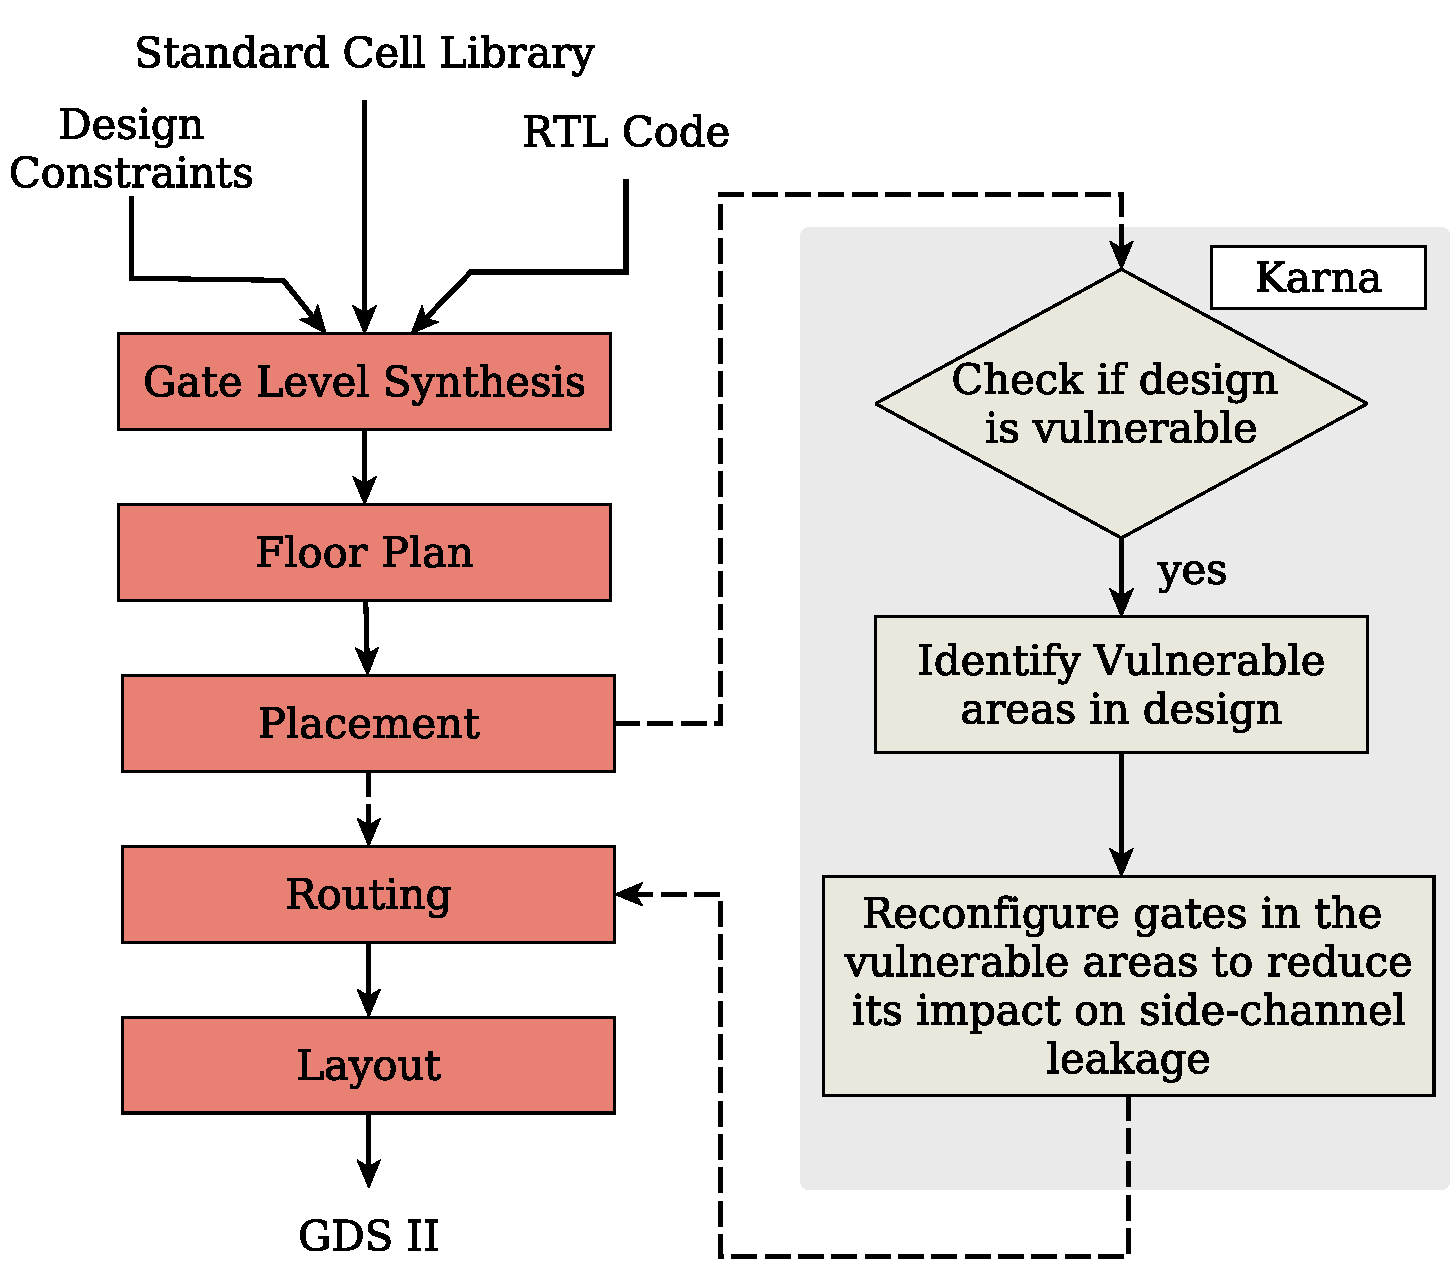
\includegraphics[scale=0.33]{Chapter4/karna.pdf}
  \caption{Figure showing the integration of {\sf Karna} into a standard EDA flow. The {\sf Karna} module inserted in the EDA flow is used to achieve side-channel security while still honoring the design's requirements in area, power, and performance.}
  \label{fig:vlsiflow}
  \vspace{-15pt}
\end{figure}

In this paper, we propose to address the side-channel security requirements of a design through the EDA flow, while still meeting other design requirements of area, power, and performance. We introduce a module called \textsf{Karna} in the EDA flow, that takes the user-specified security level as input and optimizes the parameters of the gates in the placed netlist until the desired side-channel security is achieved (Figure~\ref{fig:vlsiflow}). No specialized circuits to counter side-channel attacks are introduced during the process. The design of \textsf{Karna} is based on two critical observations. First, there are some regions in the design which contribute much more significantly to the side-channel leakage than other regions. It is sufficient to focus on these vulnerable regions in order to reduce side-channel leakage. Second, the gate-level parameters such as supply voltage, threshold voltage, and the gate size can influence the amount of side-channel leakage. 
Carefully selecting these gate-level parameters can therefore reduce side-channel leakage of the gate. 
At a high level, {\sf Karna} first identifies vulnerable regions in the design and then reconfigures the gate parameters present in these regions such that the overall side-channel leakage of the design is reduced. 
%{\sf Karna} is designed to not just achieve the security objectives of the design but also  achieve the other design objective such as area, power and performance.  


 In 2005, Tiri et al.~\cite{Verbauwhede:2005} also proposed changes to the EDA flow to prevent side-channel leakage. 
However, their scheme requires specialized gate libraries, that are not always supported by the foundry, and can considerably affect other device parameters. For example, the area of the side-channel protected AES design in~\cite{Verbauwhede:2005} increases by $3.4\times$, while the energy requirement increase by $5.9\times$. {\sf Karna}, on the other hand uses gates available in the standard cell library, and configures parameters like supply voltage, threshold voltage, and size of the vulnerable gates in order to reduce the side-channel leakage in the design phase thereby minimizing the overheads. In our work we demonstrate, using three cipher, that the area and performance and power consumption of the  designs passed through {\sf Karna} is not affected, while the side-channel leakage reduces.
The contributions of this paper are as follows.
\begin{itemize}[leftmargin=1pc]
\item We incorporate {\sf Karna} into the Synopsys design flow {M-2016 12-SP5-4} in order to pinpoint the regions in a placed netlist that contribute significantly to the side-channel leakage. 
\item We incorporate a gate-level power-optimization algorithm, which considers the side-channel security objectives of the design along with the standard design constraints such as area, power and delay.
\item {\sf Karna} provides a tunable parameter by which side-channel security can be traded off with design effort.
\item We test the efficacy of {\sf Karna} on three block cipher implementations: AES, PRESENT, and Simon. Each implementation is synthesized for a 28nm technology node. We demonstrate each design's side-channel resistance using the Test Vector Leakage Assessment (TVLA) metric~\cite{becker:2013} and show that the TVLA scores are less than 4.5 even after 100,000 measurements, while the original design requirements of power, area, and performance are unaffected.
 \end{itemize}

\noindent The outline of the paper is as follows: we introduce the necessary terminology in Section~\ref{sec:background}, motivate the need for {\sf Karna} in Section~\ref{sec:motivation} and describe it in Section~\ref{sec:proposed}. The experimental setup and results are presented in Section~\ref{sec:experiment}. The related work is discussed in Section~\ref{sec:related} and Section~\ref{sec:conclusion} concludes the paper by describing the future directions.









% \todo[inline]{can be moved to discussion section}
% Introducing security optimizations at the earlier stage of the design could cause the subsequent stages in the EDA flow to optimize or remove the changes and thereby render them useless~\cite{danger:2017}. We take into account these two constraints and integrate {\sf Karna} at the post-placement stage in the EDA flow where the delay, power and area of the design can be accurately estimated and also ensuring that the security changes are carried over into the manufactured device.


% Compared to contemporary  countermeasures~\cite{yang:2005,Singh:2017,Wang:2013,Yu:2015}, which ensure security of a manufactured device, our EDA based approach would enable fine-grained control by inserting countermeasures at the design stage itself. Further, unlike other countermeasures, which either require additional operations or new circuitry to be added, our EDA based approach would not have any such overheads. Our solution leverages the fact that EDA tools work at the gate level, which provides several tunable options like the gate's threshold voltage, size, supply voltage and load capacitance thereby enabling the design to meet a wider range of security objectives. 

%The motivation for using EDA tools for countering power analysis attacks is due to the observation that not all areas of the design contribute to the side-channel leakage. Thus, there is scope for EDA tools to optimize vulnerable regions for security. %should talk about observation
%As an example, consider Figure~\ref{fig:aes} which shows that not all areas of an AES design contribute equally to the side-channel leakage. 



%The methodology of using EDA tools to achieve side-channel security has been addressed in~\cite{Tiri:2005} where the authors introduce specialized libraries to mitigate side-channels. While this scheme efficiently eliminates side-channel leakage from the device it incurs a huge area overhead of 4$\times$~\cite{}. Our proposed scheme, on the other hand, uses the standard cell library and therefore does not incur any overheads. We achieve security by efficiently configuring the available gates.

% . The amount of effort required to characterize the library for security is very high. The points are
% \begin{itemize}
% \item Each gate is characterized for multiple corners and multiple modes so a secure library should be available for each corner and mode
% \item Number of gates increases with each node ( 330 in 32nm to 660 in 28nm).
% \item Area and delay overheads
% \item Library characterization places reliance on the foundry, no way to verify if the gate actually secures the design.
% \end{itemize}
% significant advantages over existing countermeasure techniques. 

%In this paper, we propose {\sf Karna}, a security aware module that reduces the side-channel leakage of a design. A user enables the module and specifies the desired level of security using a \texttt{security\_level} option. A high security level will cause the module to aggressively optimize the design for security. Thus a higher security level would imply a higher resistance to power analysis attacks.

%\textbf{Marked} typical EDA flow consists of several stages as shown in Figure~\ref{fig:vlsiflow}. Each stage in the flow has a specific objective to optimize one or more of the delay, power or area. The modules at each stage rely on timing and power models of the gates to achieve their objective. An EDA flow, which is security aware,  can address this objective in multiple stages. This choice can affect the other design constraints such as area, performance, and power. For example, countermeasures such as masking is incorporated in the stage 1, the high-level description stage, while gate level schemes on the other hand is incorporated in stage 2, the gate level synthesis level. Incorporating security at these stages might cause the design to incur delay and area overheads leading to the design not meeting the required area and timing constraints in the subsequent stages. Further, incorporating security in the early stages may get undone by subsequent stages. In this work, we therefore choose to introduce the {\sf Karna} module after the design is placed. At this stage, a realistic estimation of the interconnect delay and power density is known. Thus, in this stage, we can accurately gauge the impact of the proposed security based modifications on the area, delay, and performance of the device. 


%

%This security aware EDA flow is validated using an AES-128 netlist synthesized at 28nm technology. We verify the impact of our proposed flow on the area, power and delay constraints using the Synopsys Design Compiler.




%\section{Notations and Assumptions}
%\label{tbandit:notations}
\section{Background}
\label{sec:background}
In this section we first describe the metric we use to quantify side-channel leakage. We then give an overview of the power consumption of a gate and a typical EDA flow.

{\flushleft \bf Leakage Assessment:}
We use the TVLA metric as a tool to estimate side-channel leakage in {\sf Karna}. TVLA computation involves collecting two sets of power traces; one  with a fixed input and another with random inputs~\cite{becker:2013}. The statistical distance between the distributions of these two sets provides an indication of the leakage. The TVLA metric uses the Welsh t-score to compute this distance. A large magnitude of the TVLA score indicates significant side-channel leakage compared to a small magnitude of TVLA. While the prior works perform TVLA on a manufactured design, our proposed scheme integrates the TVLA methodology during the EDA flow. This enables us to perform a "white-box analysis" of the design. A device is said to pass the TVLA test if the TVLA score is less than 4.5. 



%we divide the floorplan into a $N\times N$ grid and compute the t-score for each grid. We then analyze the t-score for each grid and declare the design to be safe iff the t-scores for all the grids have an absolute value of $< 4.5$. We perform specific optimizations for the gates in the grids whose t-score is greater than 4.5.


 %However, this choice is made without taking into account the impact on the security of the design. 
%available particular configuration , at his disposal, a wide variety of configurations for the same gate. The designer chooses a particular configuration in order to meet one or more of area, performance and power requirements. The various choices for a particular gate are typically obtained by varying one of the gate parameters namely $V_t$, $V_{dd}$, load capacitance and the size of the gate. We list the impact of each parameter on the gate's power and delay consumption in Table~\ref{tab1}.




{\flushleft \bf Power Consumption of a Gate.} The  power consumption of a gate is the sum of its dynamic power $P_{dynamic}$ and static power $P_{static}$ consumption. These components are given by the following equations:
\begin{equation*}
P_{dynamic} = \alpha C_{load} V_{dd}^{2} F 
\hspace{15pt}
P_{static} =  V_{dd}\bigg( k e^{-q\frac{V_{t}}{ak_{a}T}}\bigg)\enspace. 
\end{equation*}

The dynamic power consumption of the gate is dependent on the activity factor $\alpha$, the supply voltage $V_{dd}$, the load capacitance $C_{load}$, and the operating frequency $F$. The static power consumption of the gate is dependent on the threshold voltage $V_{t}$, temperature $T$ and constants $k,q$, and $k_{a}$. The operating frequency $F$ is a parameter specified by the user in the EDA flow as a constraint, while $T$, $k,q$, and $k_{a}$ are constants. These parameters cannot be modified by the tool. On the contrary, the tool can modify $V_{dd}$, $V_{t}$, $C_{load}$, and gate size which will have an impact on the area, power, and delay of a design. 


%Modifying the other parameters will have an impact on the overall power consumption of the gate and consequently its impact on the side-channel leakage. In {\sf Karna}, for each gate we select a $V_{dd}$, $V_t$ and size value such that the TVLA is within a specified threshold. We perform this optimization while ensuring that the other design constraints like power, area and delay are not violated. \\




{\flushleft \bf Electronic Design Automation (EDA) Flow.}
A typical EDA flow consists of several stages as seen in Figure~\ref{fig:vlsiflow}. Each stage has a specific objective to optimize one or more of the delay, power or area of the design. The modules at each stage rely on timing and power models of the gates to achieve their objective. %This choice can affect the  area, delay, and power of the design. 
Current EDA flows, however, do not account for the impact of these optimizations on the security of the design. 


 In a typical EDA flow, the tool chooses a configuration for each gate from several choices that are made available by the foundry in the standard cell library. The choice is made such that the selected gate configurations meet the design requirements of area, power, and delay. Each gate configuration can be obtained by varying one or more of the supply voltage $V_{dd}$, threshold voltage $V_{t}$ and the gate $size$. For example, each gate in our 28nm standard cell library has 90 choices. Each choice can be represented using the tuple ($V_{dd}$,$V_{t}$,$size$). There are 3 choices for $V_{dd}$, 3 for $V_{t}$, and 10 choices for the $size$. Modifying one or more of these parameters may have an impact on the overall delay, power and area of the design.

To select a gate configuration, the EDA tool uses several metrics such as slack and ratio of change in power to change in delay~\cite{hu:12}. In our work, we use {\em slack}, which is defined as the difference in the required arrival time of a signal and the actual arrival time of the signal at the output of a gate. A positive slack implies that the gate has room for optimization while a negative slack implies that the timing constraint at the particular gate is violated. 

%based on the constraints specified by the designer. This choice can affect the  area, delay, and power of the design. 









%For example, countermeasures such as masking is incorporated in the stage 1, the high-level description stage, while gate level schemes on the other hand is incorporated in stage 2, the gate level synthesis level. Incorporating security at these stages might cause the design to incur delay and area overheads leading to the design not meeting the required area and timing constraints in the subsequent stages. Further, incorporating security in the early stages may get undone by subsequent stages. In this work, we therefore choose to introduce the {\sf Karna} module after the design is placed. At this stage, a realistic estimation of the interconnect delay and power density is known. Thus, in this stage, we can accurately gauge the impact of the proposed security based modifications on the area, delay, and performance of the device. 




%A typical EDA flow consists of several stages as shown in Figure~\ref{fig:vlsiflow}. Each stage in the flow has a specific objective -- optimize one or more of the delay, power or area. The modules at each stage rely on timing and power models of the gates to estimate the impact of the optimizations. %An EDA flow, which is security aware,  can address this objective in multiple stages. This choice can affect the other design constraints such as area, performance, and power. For example, countermeasures such as masking is incorporated in the stage 1, the high-level description stage, while gate level schemes on the other hand is incorporated in stage 2, the gate level synthesis level. Incorporating security at these stages might cause the design to incur delay and area overheads leading to the design not meeting the required area and timing constraints in the subsequent stages.




%mention impact of V_t, size and V_dd.
%mention how designer has freedom but that again becomes disadvantageous.


%bring out delay area and security (TVLA).

%use graph. have 3 graphs 

% \begin{table*} %add area numbers to reinforce size.
% \centering
% \begin{tabular}{|c|c|c|c|c|c|c|c|c|c|c|}
% %\toprule
% %\textbf{Treatments} & \textbf{Response 1} & \textbf{Response 2}\\
% \hline
% $V_t/ size$ & $0$ & $1$ & $2$ & $3$ & $4$ & $5$ & $6$ & $7$ & $8$ & $9$ \\ \hline
% %\midrule
% $HV_t (V_t=2)$ & 1 & 2 & 3 & 4 & 6 & 8 & 16 & 32 & 64 & 128 \\ \hline
% $RV_t (V_t=1)$ & 4 & 8 & 12 & 16 & 24 & 32 & 64 & 128 & 256 & 512 \\ \hline
% $LV_t (V_t=0)$ & 16 & 32 & 48 & 64 & 96 & 128 & 256 & 512 & 1024 & 2048 \\ \hline
% %\bottomrule


% \end{tabular}
% \caption{Table showing the variation of leakage power with $V_t$ and $size$ for an inverter.}
% \label{tab1}
% \end{table*}





%\section{Problem Definition}
%\label{tbandit:probDef}
\section{Motivation for Integrating Security requirements into an EDA Flow}
\label{sec:motivation}

%In this section, we provide a concrete example that highlights the fact that existing EDA optimizations indeed have an effect on the security of the device. 
%need for a security-aware EDA flow that optimizes security along with the typical requirements. We take an AES-128 design and synthesize it to generate six different netlists each of which is optimized to meet a different objective such as low power, high performance \& smaller area, low power \& smaller area, and high performance \& low power. % as shown in Table~\ref{tab:design}. 
%The design configurations with their area, delay, and power numbers are shown in Table~\ref{tab:design}. We then analyze the side-channel resistance of each netlist using the Mean Traces to Leak (MTL) metric defined in Section~\ref{}. %The number of power traces needed to guess the key, called mean time for disclosure (MTD), is shown in the fourth column of Table~\ref{tab:design}. A higher MTD value indicates that the attacker needs to collect large number of samples in order to guess the AES key and a smaller MTD value indicates that the device can be easily exploited via the power side-channel.

% \todo[inline]{table 1 hardly makes sense! out of 6 designs on the 3rd one actually serves the purpose.}
\begin{table}[t!]
\scriptsize
\centering

\caption{Impact of design requirements on Area, Power, Delay and the magnitude of TVLA score at the end of 4000 traces for an AES design.  }
\begin{tabular}{|c|c|c|c|c|c|}

\hline

\textbf{\begin{tabular}[c]{@{}c@{}}Design \\ Choices\end{tabular}} & \textbf{Area} & \textbf{\begin{tabular}[c]{@{}c@{}}Delay \\ (ns)\end{tabular}} & \textbf{\begin{tabular}[c]{@{}c@{}}Static\\  Power ($\mu W$)\end{tabular}} & \textbf{TVLA}\\ \hline
I -- Area $\downarrow$ Power $\downarrow$ &       78883        &                  0.48                                              &                            492.4                                  & 11.077                                                                          \\ \hline
II  -- Area $\downarrow$        &        58439       &                 0.48                                               &    602.42             &  11.41                                                                                                            \\ \hline
III -- Area $\downarrow$ Delay $\downarrow$      &       82545        &               0.47                                                 &    513.40               & 8.22  \\ \hline
IV -- Power $\downarrow$ Delay $\downarrow$     &     102256          &             0.47                                                   &               683.41     & 10.65 \\ \hline
V --    Power $\downarrow$ &    79097           &             0.48                                                   &     482.80              &   9.95\\ \hline
VI -- Delay $\downarrow$    &        91822       &        0.32                                                        &     2105.8                  &  13.97       

\\ \hline

\end{tabular}
\label{tab:design}
\end{table}
\begin{figure}[t!]
\centering
  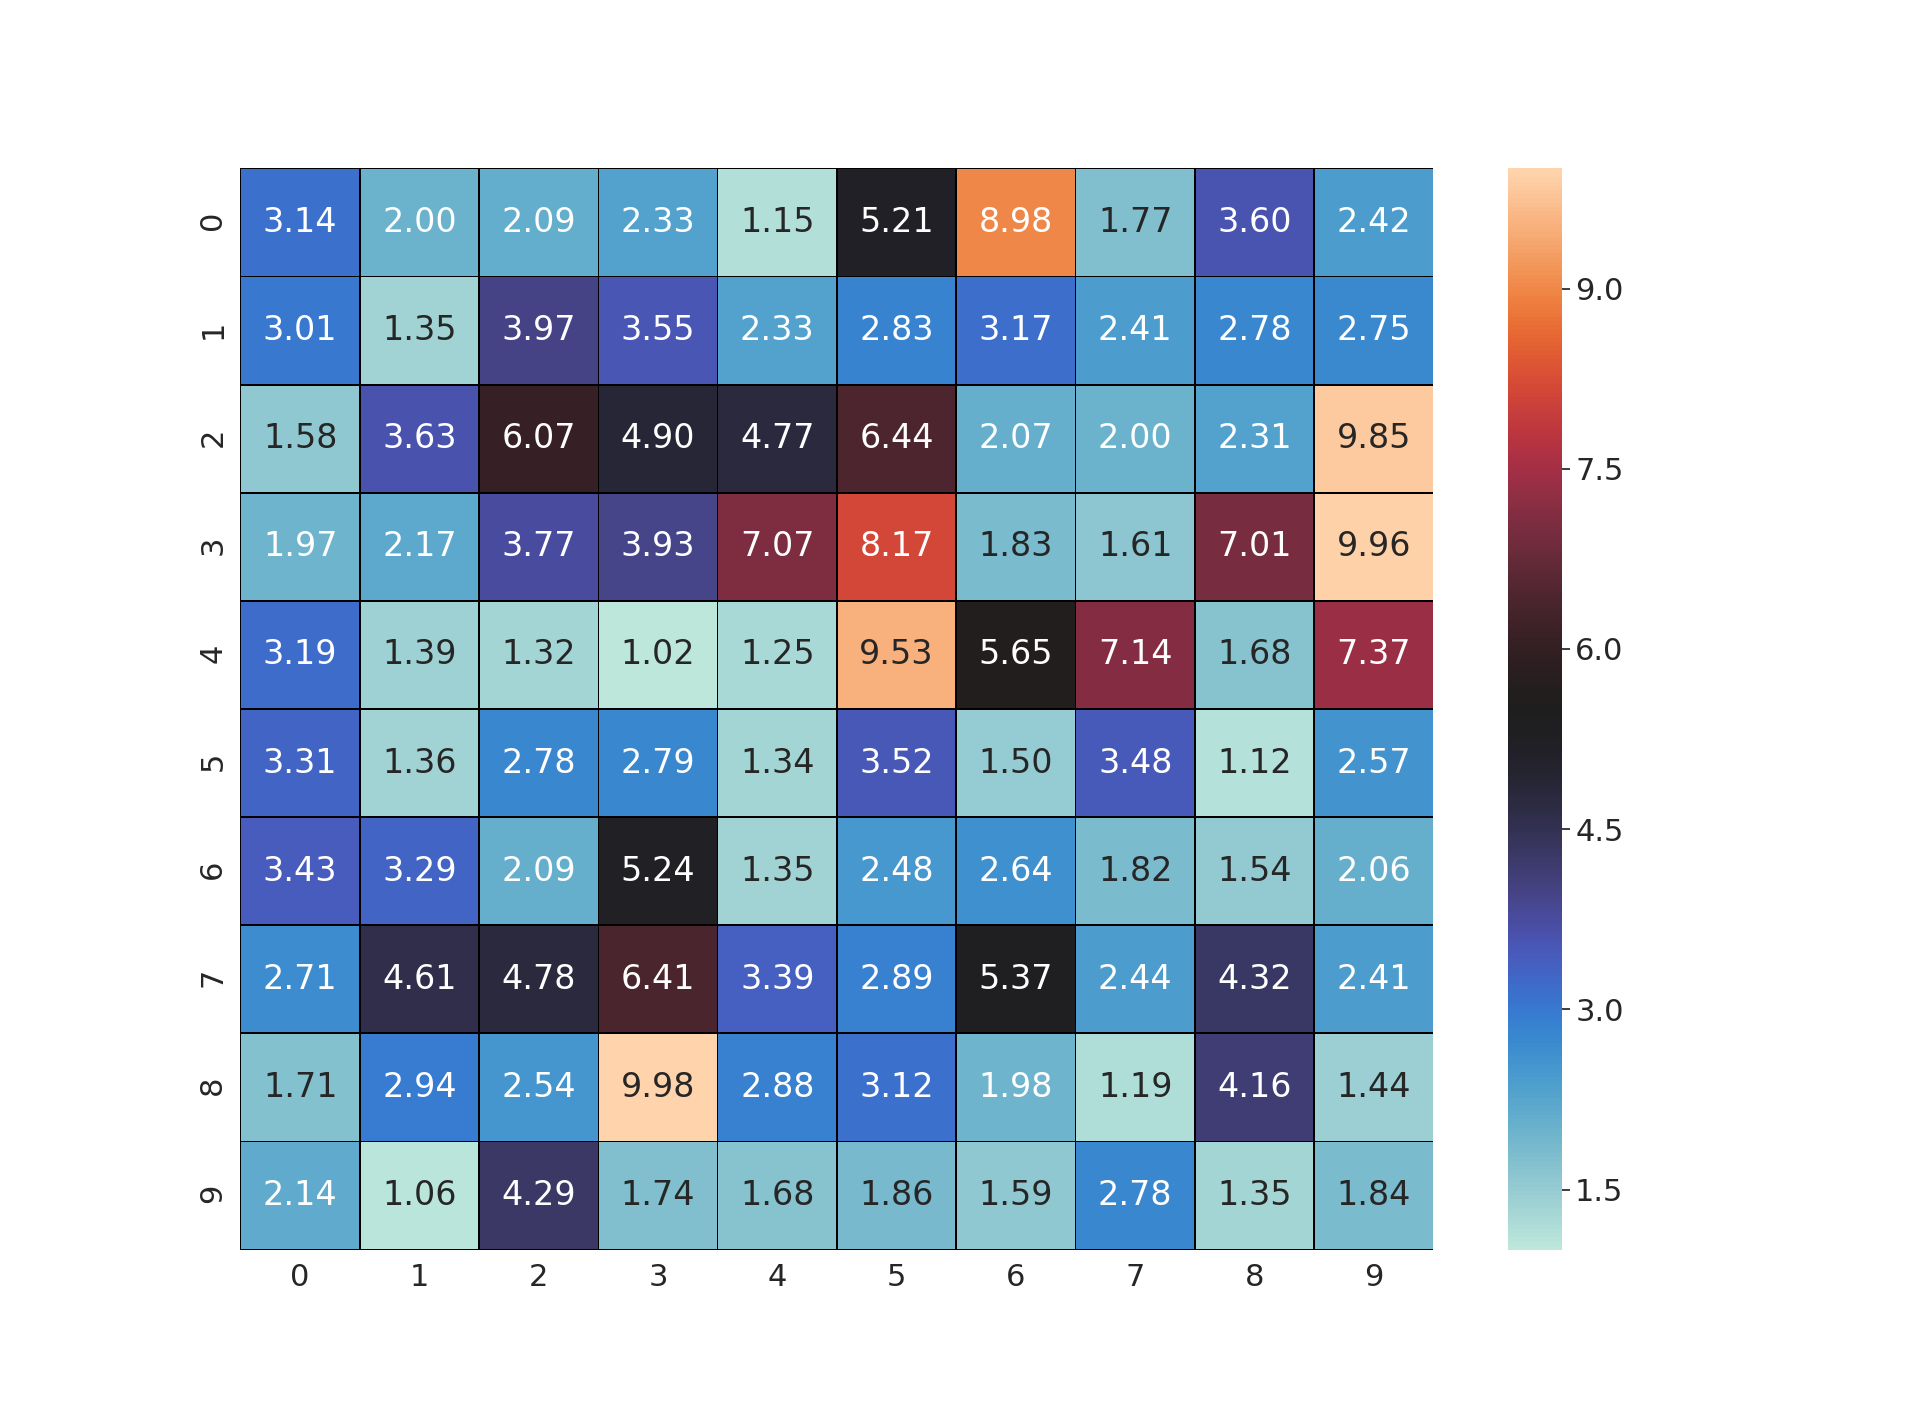
\includegraphics[scale=0.20]{Chapter4/fig/aes_before.png}  
\caption{The TVLA profile of the AES design, with the design divided into a $10\times 10$ grid and the TVLA score of each cell calculated independently. Of the 100 cells, 21 have a TVLA score greater than 4.5. The overall TVLA score of the netlist is 8.22. }
\label{fig:aesopt}
\end{figure}

In this section, we use three critical observations to motivate the use of EDA tools to achieve side-channel security.

\begin{namedthm}{Observation}
EDA algorithms influence the side-channel security of a design.
\end{namedthm}

{\flushleft We} synthesized an AES cipher to meet various design objectives. Table~\ref{tab:design} shows the area, delay, power, and security (TVLA score) of six (I to VI) different netlists. Each netlist was synthesized using the same AES design and used the same EDA tool (Synopsis Design Compiler). The EDA tool was configured with different design requirements for each synthesis. For example, netlist II was synthesized with the objective to reduce area, while netlist IV was synthesized to reduce both power and delay.
For each design, we computed the TVLA score from 4000 pairs of simulated power traces. As seen in the table, we obtain different TVLA scores for each netlist. We thus conclude that design requirements used by an EDA tool have an impact on the overall security of the final device. This experiment corroborates the observations made in~\cite{Verbauwhede:2005, danger:2017, yang:2005}. 
\begin{figure}[t!]
\centering
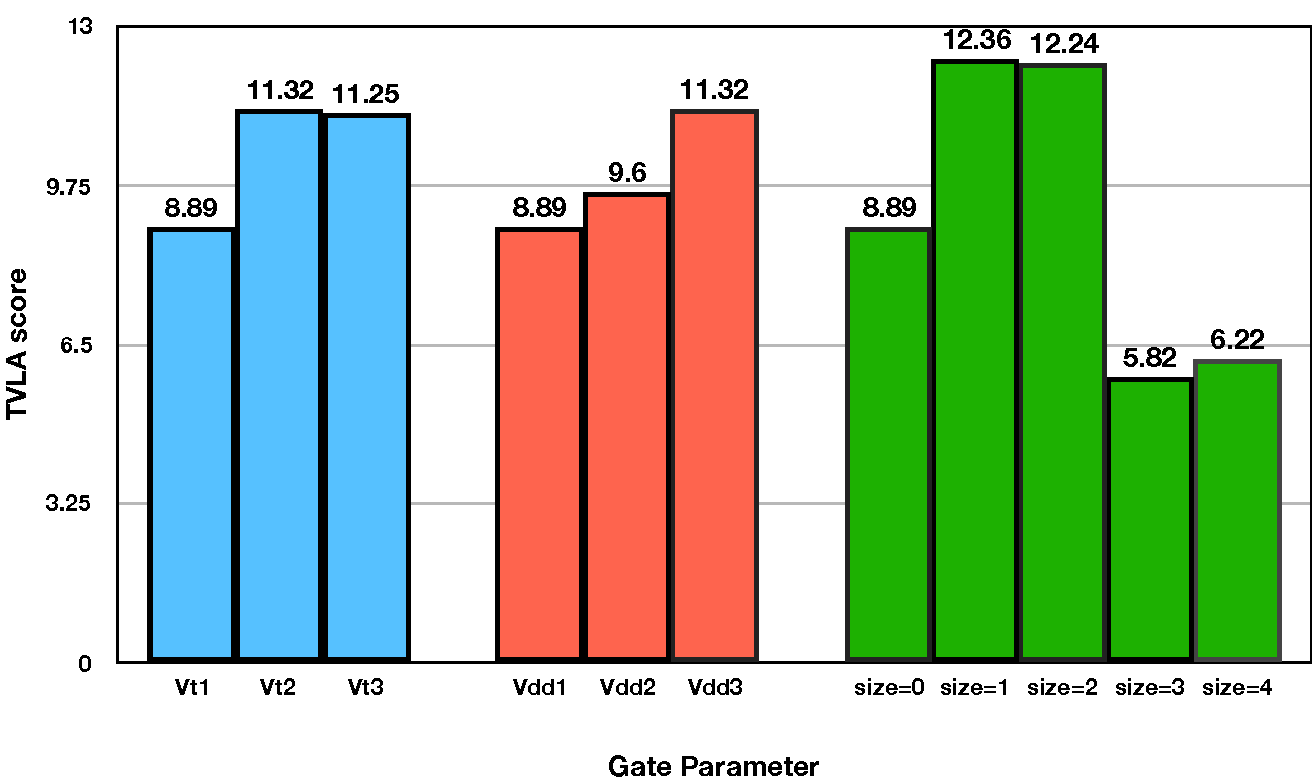
\includegraphics[scale=0.35]{Chapter4/fig/tvla_gate.pdf}
\caption{Variation of TVLA score with $V_{t}$,$V_{dd}$ and $size$ for an AND tree design.}
\label{fig:gateparam}
%\vspace{-15pt}
\end{figure}


% \begin{figure*}[ht!]
% \centering
% \begin{subfigure}{.5\textwidth}
%   \centering
%   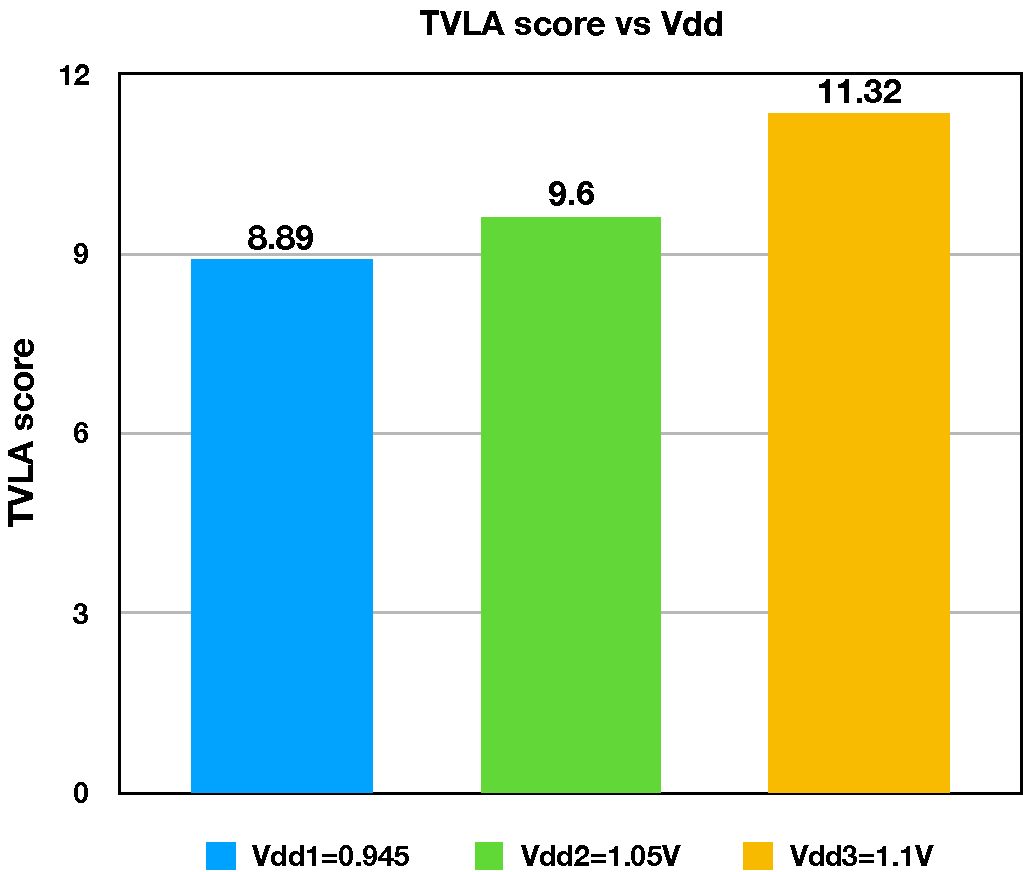
\includegraphics[width=10cm,height=5cm,keepaspectratio]{fig/tvla_vdd.pdf}
%   \caption{Variation of TVLA score with $V_{dd}$.}
%   \label{fig:sub1}
% \end{subfigure}%
% \begin{subfigure}{.55\textwidth}
%   \centering
%   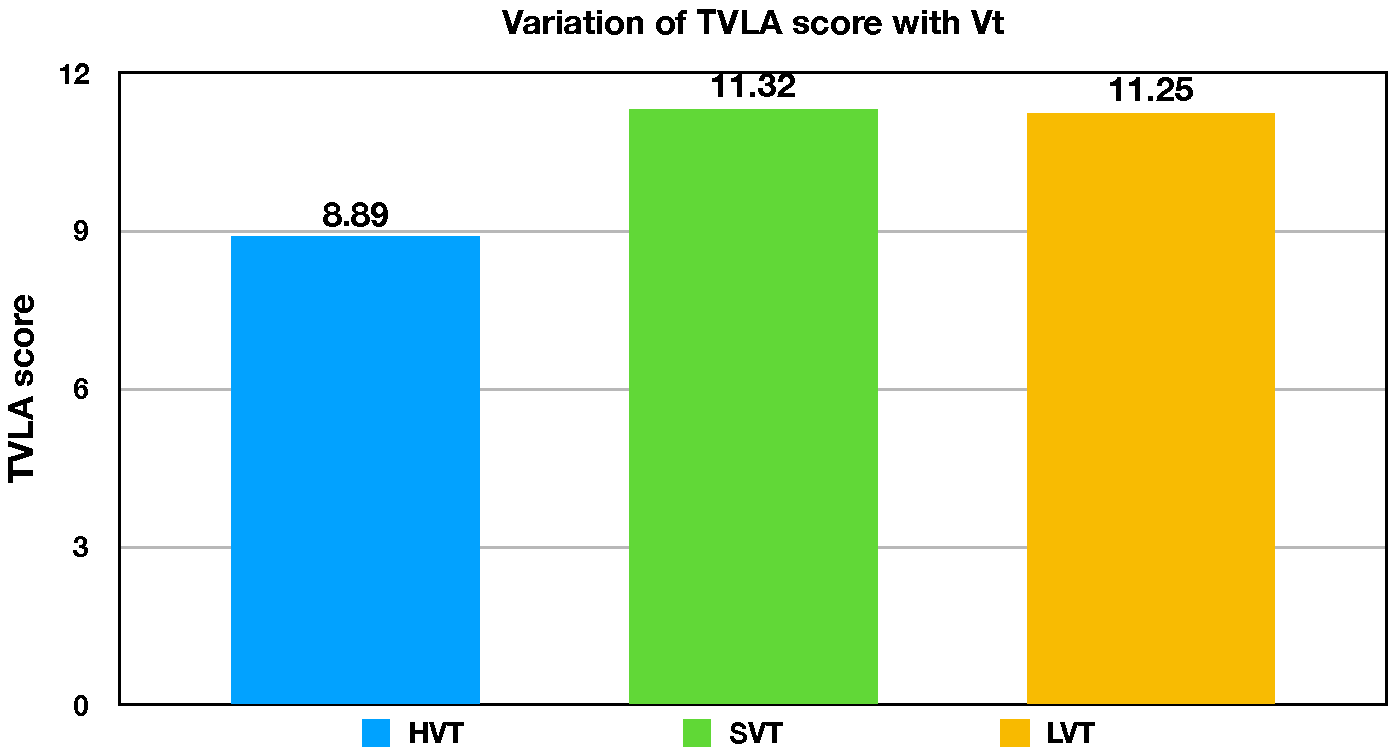
\includegraphics[width=8cm,height=5cm,keepaspectratio]{fig/tvla_vt.pdf}
%   \caption{Variation of TVLA score with $V_{t}$. }
%   \label{fig:sub2}
% \end{subfigure}
% \begin{subfigure}{.75\textwidth}
%   \centering
%   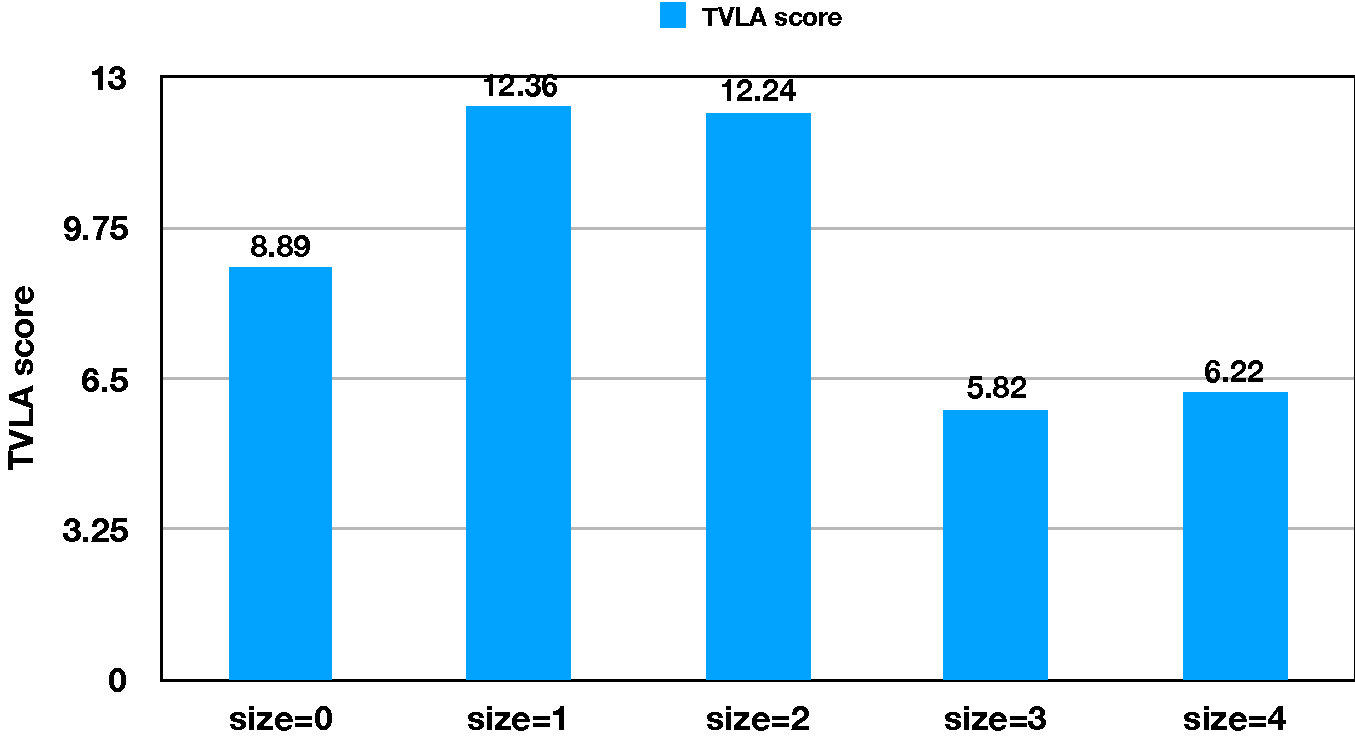
\includegraphics[width=8cm,height=5cm,keepaspectratio]{fig/tvla_size.pdf}
%   \caption{Variation of TVLA score with size. }
%   \label{fig:sub3}
% \end{subfigure}
% % \begin{subfigure}{.75\textwidth}
% %   \centering
% %   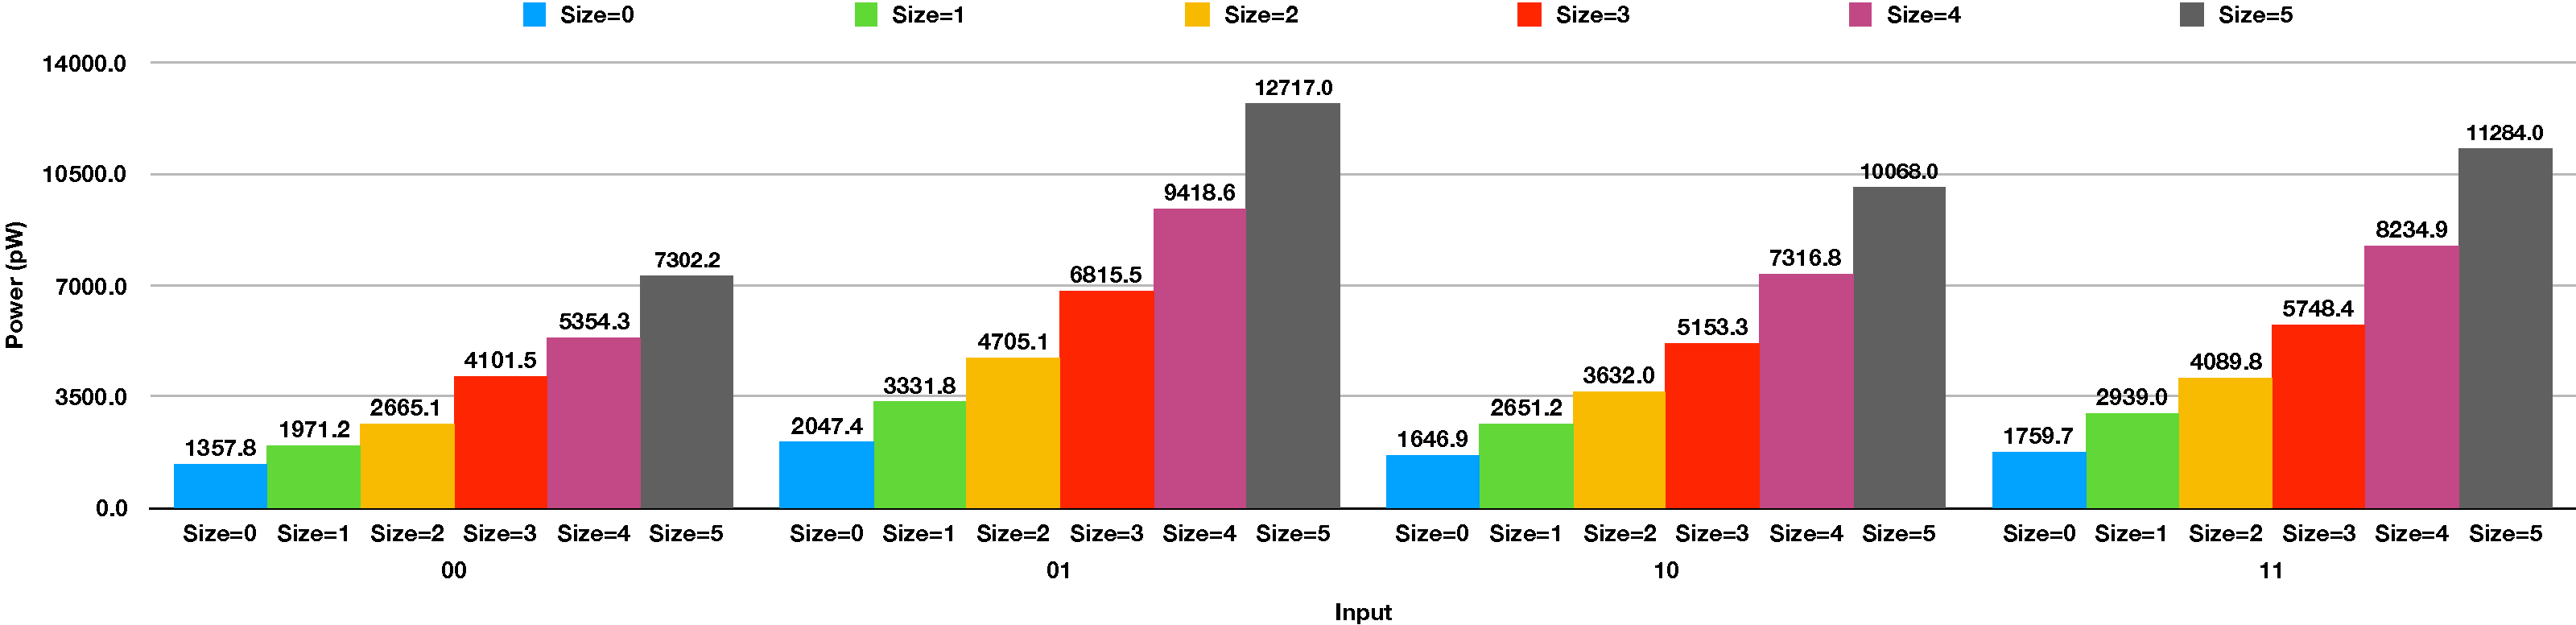
\includegraphics[width=14cm,height=5cm]{fig/sizevsinput.pdf}
% %   \caption{Variation of dynamic power of an AND gate with $size$ and logic level}
% %   \label{fig:sub3}
% % \end{subfigure}%
% % \caption{Figure showing variation of dynamic power of an AND gate with $V_{dd}$, $V_{t}$ and $size$.}
% \label{fig:power}
% \end{figure*}

% \begin{figure*}[ht!]
% \centering
% \begin{subfigure}{.5\textwidth}
%   \centering
%   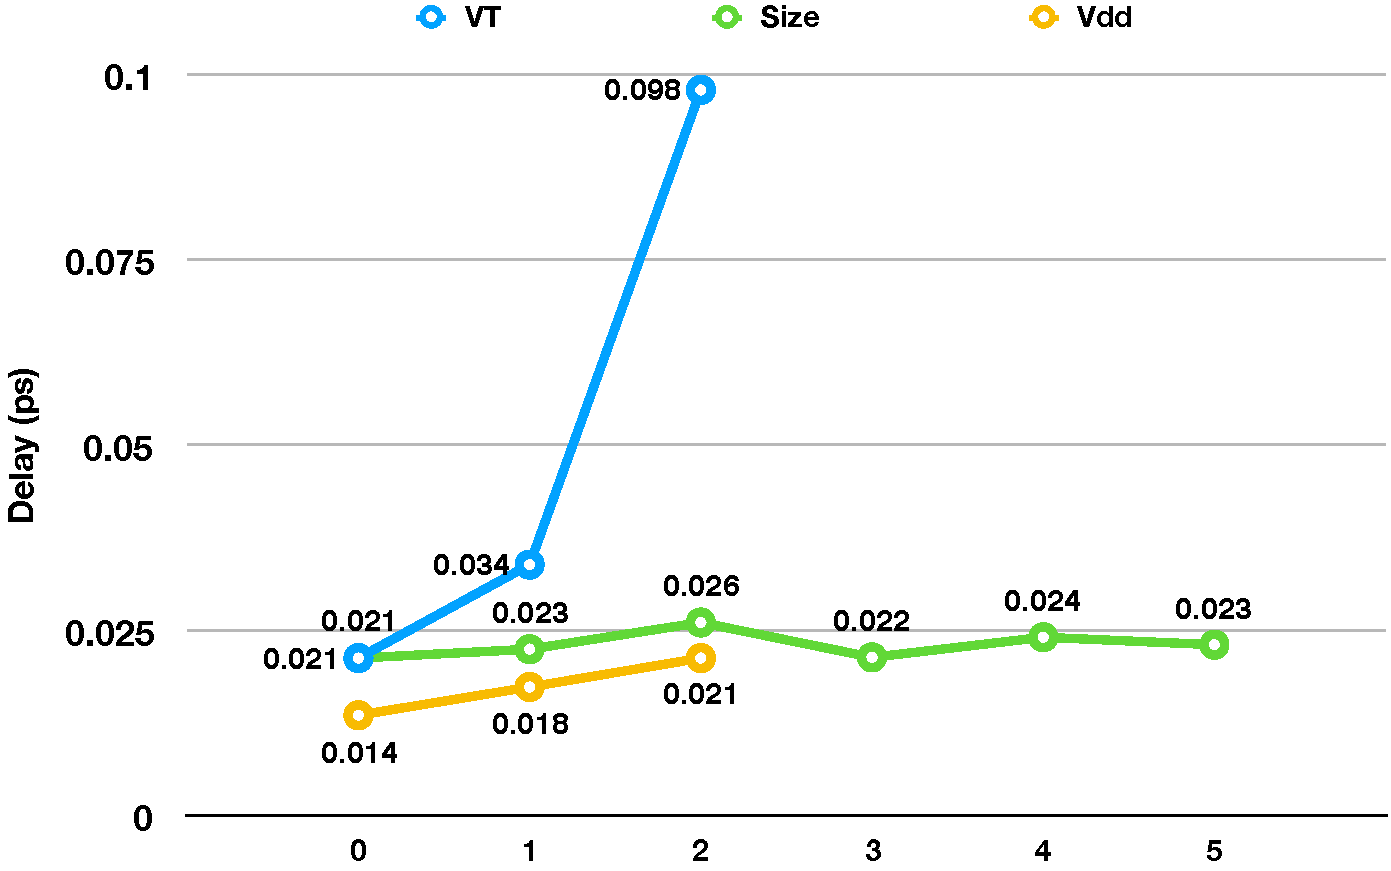
\includegraphics[width=10cm,height=5cm]{fig/delayvariation.pdf}
%   \caption{Variation of delay of an AND gate with $V_{dd}$,$V_{t}$ and $size$.}
%   \label{fig:delay1}
% \end{subfigure}%
% \begin{subfigure}{.55\textwidth}
%   \centering
%   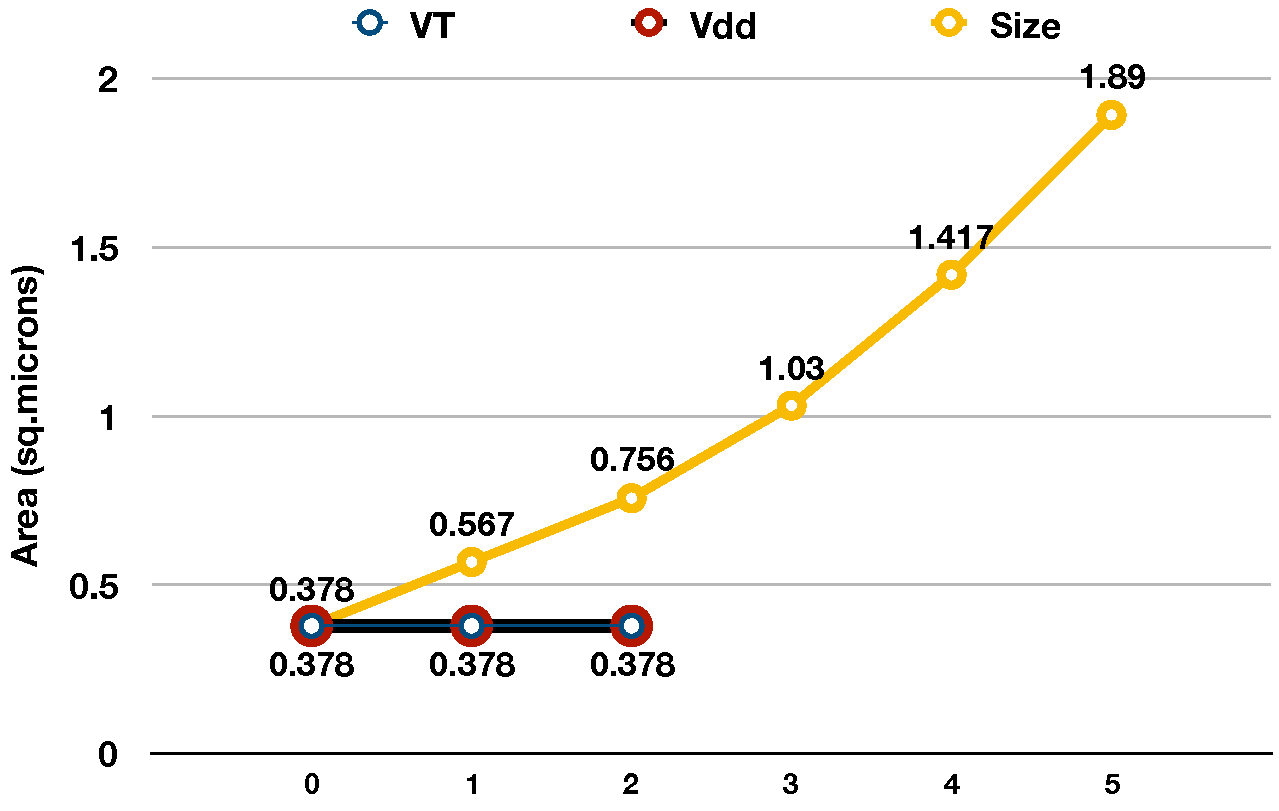
\includegraphics[width=8cm,height=5cm]{fig/areavariation.pdf}
%   \caption{Variation of area of an AND gate with $V_{dd}$, $V_{t}$ and $size$. }
%   \label{fig:delay2}
% \end{subfigure}
% \caption{Figure showing variation of delay and area of an AND with respect to $V_{dd}$, $V_{t}$ and $size$. It can be seen that delay increases with increase in $V_{dd}$, $V_{t}$ and size while area remains constant for $V_{dd}$ and $V_{t}$ scaling and increases with increase in size}
% \label{fig:delay}
% \end{figure*}


\begin{namedthm}{Observation }
Not all regions of the synthesized design contribute equally to the leakage.
\end{namedthm}
{\flushleft There} are certain areas in the design that have a higher leakage compared to other areas. In order to evaluate this, we divided the netlist into a $10 \times 10$ grid and computed the TVLA score for each region independently, thus obtaining 100 different TVLA scores corresponding to various regions in the  netlist. Figure~\ref{fig:aesopt} shows the variations in the TVLA score calculated for netlist III. 
{\sf Karna}, reconfigures the units where leakage is high, so as to reduce the overall side-channel leakage of the design without compromising the other design requirements. 


\begin{namedthm}{Observation }
The side-channel leakage from a gate depends on its  parameters.
\end{namedthm}
In order to observe the impact of each gate configuration on the side-channel leakage, we synthesized an AND-tree design with 16-bit input and 1-bit output, multiple times with different gate configurations. Each synthesis run was done with a different gate configuration. Figure~\ref{fig:gateparam} shows the TVLA scores obtained from 2000 pairs of simulated power traces for each run. It can be seen that changing 
$V_{dd}$, $V_t$ or $size$ options for a gate has an impact on the side-channel leakage of the design.

%Hence, it is important to select gate configurations that meet the design requirements but do not impact the security constraint.
%As mentioned earlier, the EDA tool optimizes the $V_{dd}$, $V_{t}$ and  size of each gate in the design in order to meet a given constraint.We now examine the impact of modifying the design choices by using an AND gate as an example. Figure~\ref{fig:power} shows the variation of dynamic power of an AND gate when the supply voltage $V_{dd}$ and threshold voltage $V_{t}$ are varied. It can be seen that increasing the supply voltage will cause the power consumed by the gate to increase by $\approx5\times-20\times$. We can also observe that the power consumed for different inputs (i.e, $00$, $01$, $10$, and $11$) is different. For example, the difference in the power consumed for inputs $11$ and $01$ at $V_{dd}=1.1V$ is $288$ pW, whereas the difference is $3.5$ pW at $V_{dd}=0.945V$. Such differences can be leveraged to distinguish between the inputs provided at the AND gate and may affect the overall security of the design. A similar observation can be made in figure~\ref{fig:sub2} for $V_{t}$ and figure~\ref{fig:sub3} for varying the gate size. 

A na\"ive approach to achieve security would be to choose gate configurations that provide highest security. However,  na\"ively choosing such gate configurations may violate other design requirements such as delay and power. 
Therefore, there is a need for a careful strategy to vary the gate parameters such that the overall security of the design improves while still meeting the desired design requirements.  
\vspace{-3pt}
% Motivation for post-placement
%It is important to note that the security countermeasures incorporated at any given stage should remain persistent throughout the other stages in the flow. For example, incorporating security at a post-synthesis stage might cause the design to violate area requirements in the placement stage thus requiring re-synthesis. Another consequence is that the tool could optimized out the proposed countermeasures thereby rendering them ineffective. 
%In this work, we therefore choose to introduce the {\sf Karna} module which selects the appropriate gate configuration for each after the design is placed. At this stage, a realistic estimation of the interconnect delay and power density is known. Thus, in this stage, we can accurately gauge the impact of the proposed security based modifications on the area, delay, and performance of the device. 

% a gate $g_{i}$ to be in the critical path of a design iff }




%The problem of securing devices against power side channel attacks has been explored since \cite{} and \cite{}. Techniques like \cite{} and \cite{} have explored software level and device level techniques to address this issue. However, software level techniques only alleviate the symptoms but fail to address the root cause of such vulnerabilities. Device level techniques rely on modifying the physical traits of the device either at gate level as in \cite{}. In this work we explore an alternative idea of mitigating power side-channels at the design level. We motivate the need for such a technique in this section. %This is what disconnected writing gets you, you idiot!

%\indent A power side-channel is said to occur when the device under test consumes drastically different power for a specific input vector than for other random inputs. Mitigating this problem would mean producing a configuration for the device such that it consumes constant or near constant amount of power for any input thereby reducing the statistical variation between the power signature for a fixed input. In device terms this would mean assigning each gate in the device a configuration such that the overall power consumption is fairly constant. 

%\indent In a typical VLSI design flow, the device typically undergoes several optimizations, each with its own objective. The primary of these requirements is performance. The recent power wall and the need for compact devices has led to the emergence of power and area as additional requirements. However, it should be noted that power and area are optimized only if the primary objective is satisfied. 

%\textbf{Observation 1: This drive for a performance optimized design cause the designers to pick gate configurations that, while making the design efficient, might make it compromise the security of the device.}

%It can be seen that while the various algorithms in the EDA flow optimize the design for one or more of performance,area or power, none of them consider the impact on the overall security of the device. This causes the algorithms to pick gate configurations that, while making the design optimal with respect to its requirements, lower the MTD of the device. 





% \indent When we observe the overall power consumption of the device, it can be divided into two components viz. static and dynamic power consumption. Static power is the power that the device consumes during the idle stage and is influenced by temperature, Threshold voltage ($V_t$) and the size of the gate ($g^i_s$). Dynamic power, is the power that is consumed when the device performs some computation, and is affected by the load capacitance ($C_i$), supply voltage $V_(dd)$, and the operating frequency ($F$). It is interesting to see the impact of modifying one or more of these device parameters on the power side-channel of the device.

% \indent Table~\ref{tab2} and~\ref{tab3} shows the leakage power and dynamic power of an inverter. It can be seen that varying $V_t$, $size$, $V_(dd)$ and load capacitance of a gate has an impact on the amount of power that the gate finally consumes. 
% \begin{table}[!ht]
% \begin{tabular}{|c|c|c|c|}
% \hline
% \textbf{Logic Level} & \textbf{$V_{(dd)_1}$} & \textbf{$V_{(dd)_2}$} & \textbf{$V_{(dd)_3}$} \\ \hline
% 00                   &               &               &               \\ \hline
% 01                   &               &               &               \\ \hline
% 10                   &               &               &               \\ \hline
% 11                   &               &               &               \\ \hline
% \end{tabular}
% \label{tab2}
% \caption{Table showing the impact of $V_(dd)$ on the power consumed.}
% \end{table}

% \begin{table}[!ht]
% \begin{tabular}{|c|c|c|c|}
% \hline
% \textbf{Logic Level} & \textbf{$V_{t_1}$} & \textbf{$V_{t_2}$} & \textbf{$V_{t_3}$} \\ \hline
% 00                   &               &               &               \\ \hline
% 01                   &               &               &               \\ \hline
% 10                   &               &               &               \\ \hline
% 11                   &               &               &               \\ \hline
% \end{tabular}
% \label{tab3}
% \caption{Table showing the impact of $V_t$ on the power consumed.}
% \end{table}
% It can be seen that varying $V_t$, $size$, $V_(dd)$ has an impact on the amount of power a gate consumes and thereby it also impacts the power side channel of the entire device. Hence there exists the need for a optimization scheme that takes into account the security of the device. In the next section we introduce Karna, a security aware power optimization scheme.




% %\indent Table~\ref{tab4} shows the various requirements that are addressed during the design manufacturing, it can be noted that security is never viewed as an objective during these stages. This is because quantifying the security or degree of "trust" in a chip is a hard problem to solve in itself. It is harder to quantify the "change" in the degree of trust due to an optimization. Figures~\ref{fig1} and ~\ref{fig2} represent two different optimization choices performed on the same design. It can be seen that 

% %\textbf{Observation 3: There exists a need to reliably quantify the impact of a design optimization on the security of the device.}

% %It can be seen that there exists a need for a design level solution that is able to quantify the impact of design optimizations on security. This will enable designers to explore security aware design optimizations such that performance goals can be achieved while minimizing the vulnerability of the device. In the next section, we will explore how existing metrics can be translated %find a better word
% %into design level requirements and a security aware power minimization scheme. 




%section{Motivation}
%\label{tbandit:motivation}
\begin{table}[t!]
\scriptsize
\centering
\caption{Design delay, area and power numbers with and without {\sf Karna} for achieving a security ($\tau$) of 4.5.}
\label{tab:tvla}
\begin{tabular}{|p{1.2cm}|p{0.8cm}|p{0.8cm}|p{0.8cm}|p{0.8cm}|p{0.8cm}|p{0.8cm}|}
\hline
\multicolumn{1}{|l|}{\multirow{2}{*}}                              & \multicolumn{2}{c|}{\textbf{AES}}     & \multicolumn{2}{|c|}{\textbf{PRESENT} }  & \multicolumn{2}{|c|}{\textbf{Simon}}  \\ \cline{2-7} 
\multicolumn{1}{|l|}{}                                               & \textbf{\begin{tabular}[l]{@{}l@{}}Without \\ {\sf Karna}\end{tabular}} & \textbf{\begin{tabular}[l]{@{}l@{}}With\\ {\sf Karna}\end{tabular}} & \textbf{\begin{tabular}[l]{@{}l@{}}Without \\ {\sf Karna}\end{tabular}} & \textbf{\begin{tabular}[l]{@{}l@{}}With\\ {\sf Karna}\end{tabular}} & \textbf{\begin{tabular}[l]{@{}l@{}}Without \\ {\sf Karna}\end{tabular}} & \textbf{\begin{tabular}[l]{@{}l@{}}With\\ {\sf Karna}\end{tabular}}  \\ \hline
\textbf{Delay (ns)}                                                  & 0.5                                                                      & 0.5                                                                    & 0.3                                                                     & 0.3                                                                     & 1.12                                                                     & 1.12                                                                   \\ \hline
\textbf{\begin{tabular}[l]{@{}l@{}}Leakage\\Power($\mu$W)\end{tabular}}                                           & 492.4                                                                    & 236.65                                                                 & 5.62                                                                    & 0.418                                                                   & 3.70                                                                     & 0.16                                                                   \\ \hline
\textbf{\begin{tabular}[l]{@{}l@{}}Area\\  Utilization\end{tabular}} & 60\%                                                                     & 80\%                                                                   &          60\%                                                               &        81.8\%                                                                 &                             60\%                                             &        64.67\%                                                                \\ \hline 
\textbf{\#Gates}                                                     & 149943 & 149943                                                                                                                      & 1520 & 1520                                                                                                                         & 622  & 622                                                                                                                        \\ \hline
\textbf{Total Area (sq.microns)}  & 99651.67  &  99651.67 & 1596.9 & 1596.9 & 1240.3 & 1240.3 \\ \hline
\textbf{TVLA}                                                        & 8.22                                                                     & 3.7                                                                    & 12.28                                                                   & 4.06                                                                    & 20.799                                                                   & 4.48                                                                   \\ \hline
%\textbf{#Grids} &  & 100 &   & 1 &  & 1 \\ \hline

\end{tabular}
\vspace{-10pt}
\end{table}
\section{Implementation and Results}
\label{sec:experiment}
We use implementations of the AES\footnote{$https://opencores.org/projects/tiny\_aes$}, PRESENT\footnote{$https://opencores.org/projects/present$} and Simon\footnote{$https://opencores.org/projects/simon\_core$} ciphers to evaluate {\sf Karna} algorithm. For AES we set the grid size to $10\times 10$. PRESENT and Simon are very small designs, therefore a grid size of $1\times 1$ suffices.
The designs are synthesized using a 28nm standard cell library, which offers 3 $V_{dd}$ choices, 3 $V_t$ choices and 10 $size$ choices, thus a total of 90 configurations for every gate. We synthesize the designs for maximum performance using Synopsys design compiler version \texttt{M-2016.12-SP5-4} and use the Cadence innovus tool \texttt{v16.21-s078\_1} to place and route the design by setting the area utilization at 60\%. 

 The {\sf Karna} algorithm is implemented in C++. The implementation uses boost graph library version 1.58 to represent the netlist as a graph and the standard cell library to annotate the various power, delay and area information to each node. {\sf Karna} uses the power traces obtained from Synopsys PrimeTime \texttt{M-2017.06-SP2} to compute the TVLA. Each TVLA computation uses 4000 pairs of power traces for fixed and random test inputs. Based on the TVLA scores, the implementation identifies vulnerable gates and reconfigures them. It then invokes OpenTimer~\cite{Opentimer} to validate each reconfiguration.

 Table~\ref{tab:tvla} shows the properties of the synthesized netlist with and without {\sf Karna}. {\sf Karna} is able to achieve the desired level of security ($\tau=4.5$) in all three designs without any impact on delay, leakage power and the number of gates. While the total area of the chip remains the same, the area utilization increases by about 20\% for AES and PRESENT; and is negligible  for Simon. Figure~\ref{fig:aesfinal} shows the TVLA scores for various regions in the AES layout optimized for security using  {\sf Karna} after 100,000 power trace measurements.  Unlike the unoptimized AES layout (Figure~\ref{fig:aesopt}), we find no region having a TVLA score greater than 4.5.
 
The run time for the EDA flow with {\sf Karna} enabled is 3 days for AES and around 6 hours each for PRESENT and Simon on a 4-core Intel Xeon E5-1620 processor with 32 GB RAM. Almost 96\% of the time is taken up in collecting power traces for TVLA computation.
This is mainly because the TVLA computation in each iteration requires 8000 power traces to be simulated with different test vectors. This time  can be reduced by parallelizing trace collection.
%\vspace{-3pt}


%The EDA runtime depends considerably on the user specified security level $\tau$. A low value implies that the design is expected to meet strict security standards. This implies more regions in the netlist fail and consequently the module has to reconfigure a lot more gates. Figure~\ref{fig:tvla} shows that the number of grids that fail increases considerably as $\tau$ reduces. Thus for a small value of $\tau$, the algorithm will take longer to complete. 

%{\flushleft \bf Limitations of {\sf Karna}} The algorithm depends on the power traces to identify the vulnerable regions in each iteration. This trace collection drastically increases the runtime of the algorithm. For example, for the AES design, 73 minutes were spent in the EDA flow and 87 minutes were spent in the reconfiguration, however the trace collection took 3 days. In our future we explore methods to reduce this large time.



%Since, {\sf Karna} only reconfigures the gates in the netlist the overall gate count also remains constant. 


%The command allows for varying the granularity at which the dynamic power is calculated, and hence the TVLA analysis can be performed at any level the designer prefers. We set the security level to 4.5 and use a grid size of 100. 




% We use boost graph library. Each node in the graph has the following properties: node id, node type which could be a primary input/output or cell type, node slack, arrival time, output capacitance, number of gates driven by the particular node (fanouts), number of gates driving the particular node, $V_{dd}$, $V_t$, $size$, TVLA score. A node is marked unsafe if it belongs to a grid that has a high TVLA score and safe otherwise. A node is marked critical if it has timing violations or if it cannot be optimized further i.e, reconfiguring the node could lead to timing, slew or capacitance violations. The values of delay, leakage power and dynamic power are calculated based on the node type,$V_{dd}$, $V_t$ and $size$. %\cite{OpenTimer} has options for performing both full and incremental static timing analysis. We use the full STA option for our experiments. 

% The TVLA calculation was run on a 128-thread, 32-core dual socket AMD EPYC 7601 32-Core Processor. We sped up the trace collection by using the set\_host\_options command in primetime. 



% %describe the experimental setup.
% The AES netlist is synthesized using the 28nm netlist. Synopsys dc compiler version M-2016.12 was used to synthesize the netlist. The netlist has 150,000 gates The \textit{set\_max\_delay} option was used to ensure that the design is timing optimized. The target frequency was set at 0.5ns. The device is then placed and routed using innovus tool from cadence. 

% Around 40,000 traces are generated for the fixed and the varying inputs. The dynamic power calculation was done using synopsys primetime. The sampling was done using the \textit{read\_vcd} command in primetime. The command allows for varying the granularity at which the dynamic power is calculated, and hence the TVLA analysis can be performed at any level the designer wishes. The samples were collected using the experimental procedure described in \cite{}. 

%\section{Results}
% \todo{
% Include Present and Simon speck results. 
% }
\label{sec:results}

% We tested the {\sf Karna} algorithm on the following ciphers AES-128, Simon and PRESENT. Table~\ref{tab:tvla} shows the impact of {\sf Karna} algorithm on the design requirements such as Delay, Power and Area. It can be seen that overall 
% Figure~\ref{tvla} shows the variation in t-score with sample sizes. X-axis represents the number of samples while the Y-axis represents the t-score. It can be seen that the t-score crosses 4.5 even with 1000 samples. Figure~\ref{fig2} shows the t-score for each grid with 1000 samples. It can be seen that 21 grids fail out of the 100 grids. The gates belonging to these grids are considered for the optimization stage. Table ~\ref{tab:tvla} shows the variation in leakage power, delay, area of the netlist before and after optimization. 
% Please add the following required packages to your document preamble:
% \usepackage{graphicx}
% Please add the following required packages to your document preamble:
% \usepackage{multirow}






% Please add the following required packages to your document preamble:
% \usepackage{multirow}









% \begin{table*}[t!]
% \centering
% \caption{Table showing the delay, area and power numbers before and after optimization. While the area of the netlist increases, the total die area remains the same and hence the overall area of the manufactured device remains the constant.}
% \label{tab:tvla}

% \begin{tabular}{|c|c|c|}
% \hline
% \textbf{Parameter} & \textbf{\begin{tabular}[c]{@{}c@{}}Unoptimized \\ Netlist\end{tabular}} & \textbf{\begin{tabular}[c]{@{}c@{}}Optimized\\ Netlist\end{tabular}} \\ \hline
% \textbf{Delay(ns)} & 0.5 & 0.5 \\ \hline
% \textbf{Area(sq.microns)} & 59791 & 101502   \\ \hline
% \textbf{Static Power($\mu$W)} & 492.4  &  236.65  \\ \hline
% \textbf{TVLA score} & 8.22 & 3.7 \\ \hline
% %\textbf{Dynamic Power (mW)}
% \textbf{Total Number of Gates} &\multicolumn{2}{|c|}{149943} \\ \hline
% \end{tabular}%
% \end{table*}
%\subsection{Runtime Optimizations of {\sf Karna}}
% As mentioned in Section~\ref{sec:proposed}, the number of STA calls can have an impact on the overall runtime of the algorithm. In order to reduce the number of STA calls, we use an adaptive gate replacement policy used in~\cite{MLtimer} in order to speed up the {\sf Karna} module. Figure~\ref{fig:runtime} shows the speedup achieved by employing this gate replacement policy. It can be seen that adaptive window sizing policy is $\approx5\times$ faster than the greedy replacement policy. This is because the order in which the gates get replaced remains fairly constant for most of the iterations, an observation which we leverage to converge to an optimal solution faster.

\begin{figure}[t!]
\centering
  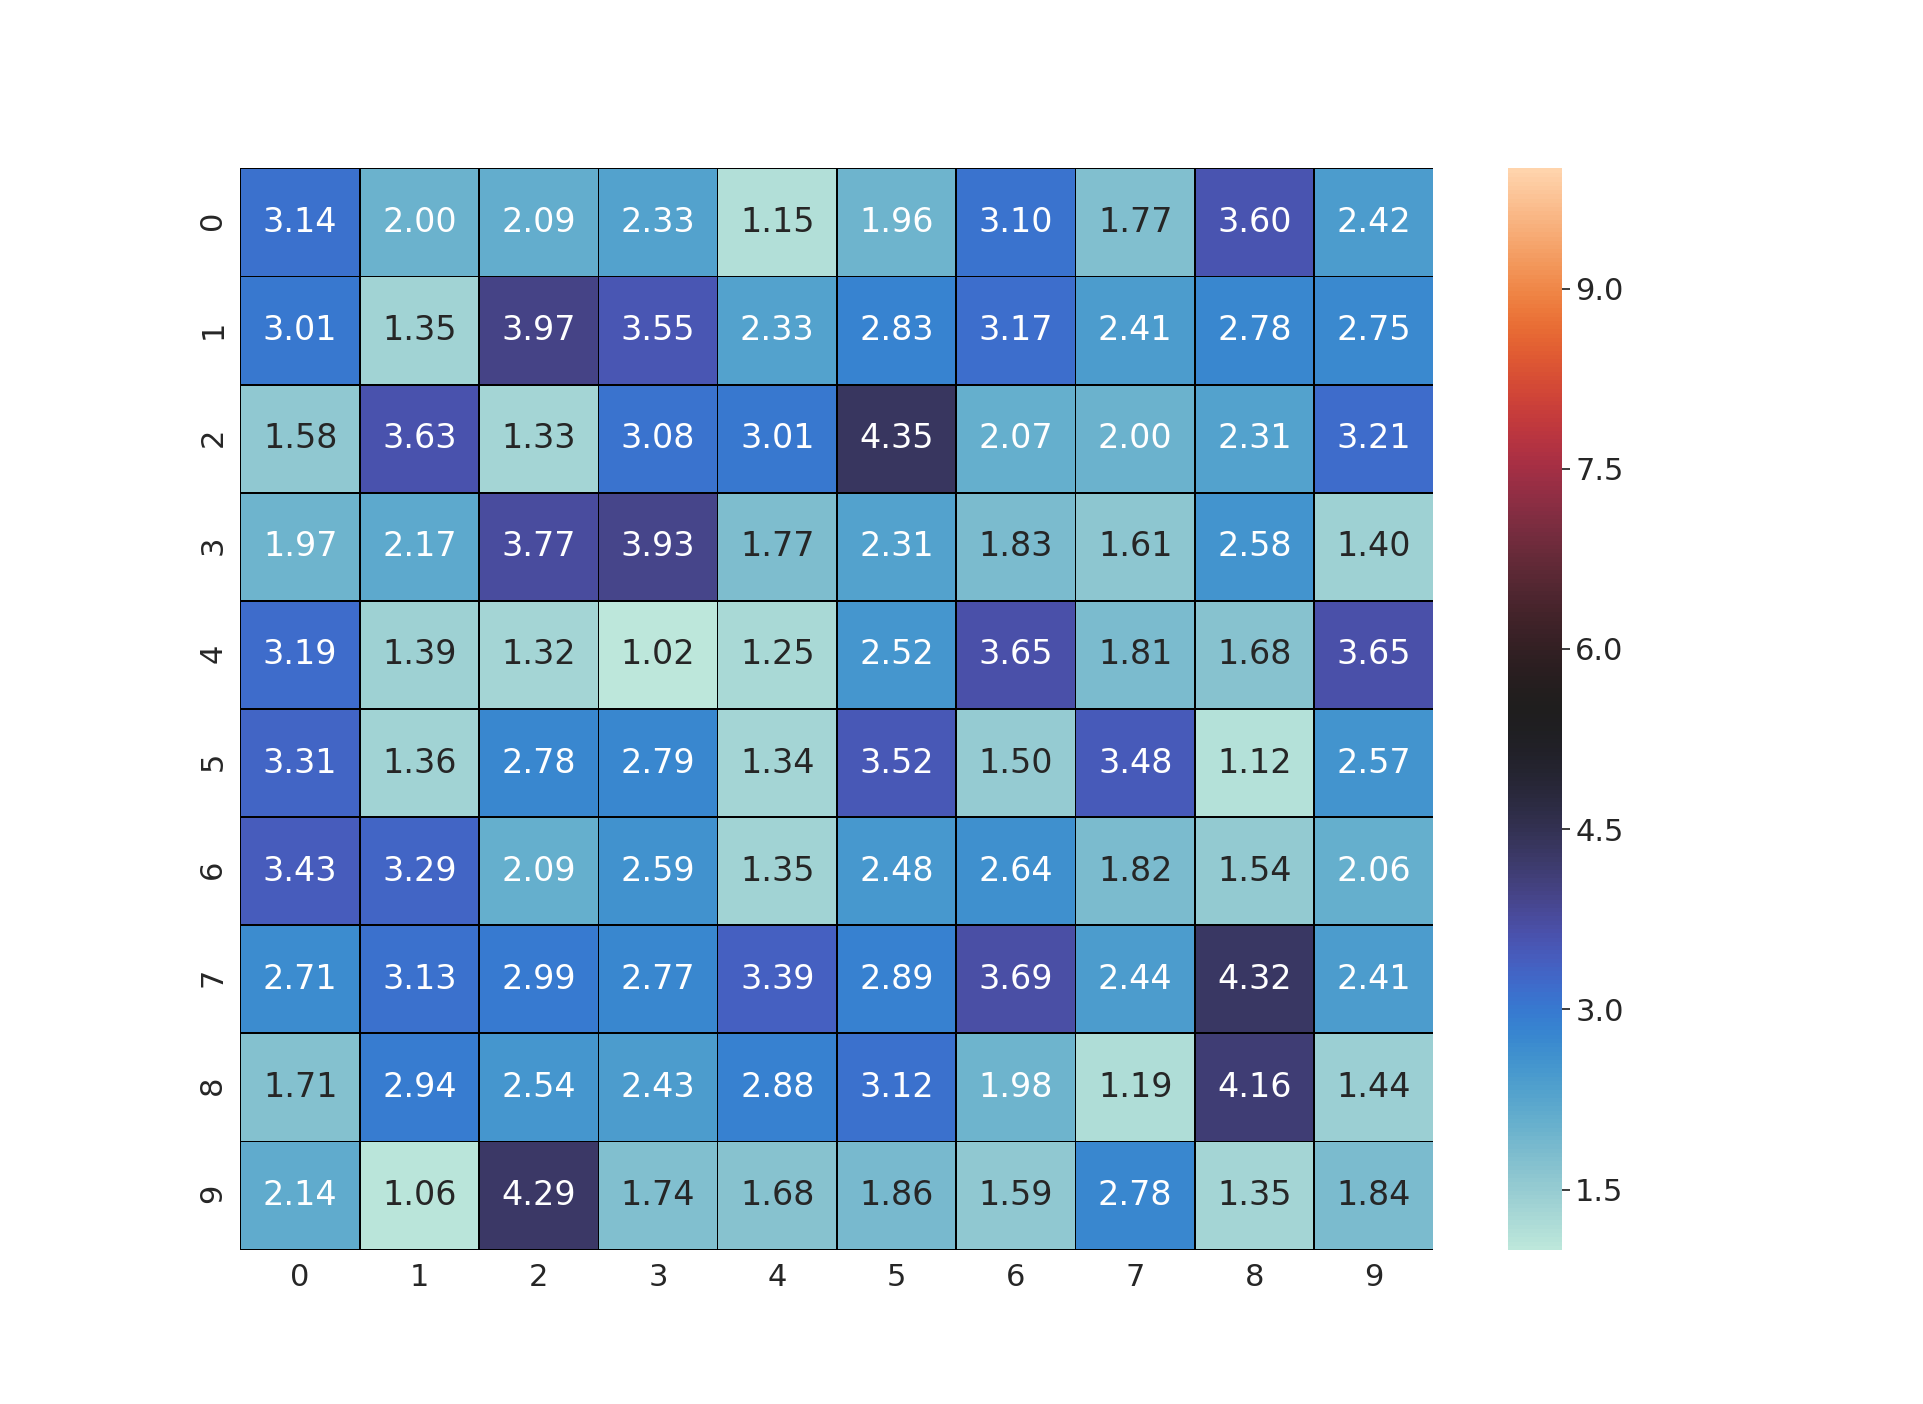
\includegraphics[scale=0.20]{Chapter4/fig/aes_final.png}  
\caption{The TVLA profile of the AES-128 design, with the design divided into a $10\times 10$ grid after {\sf Karna} optimization. }
\label{fig:aesfinal}
\vspace{-10pt}
\end{figure}


% \begin{figure}[t!]
% \centering
% 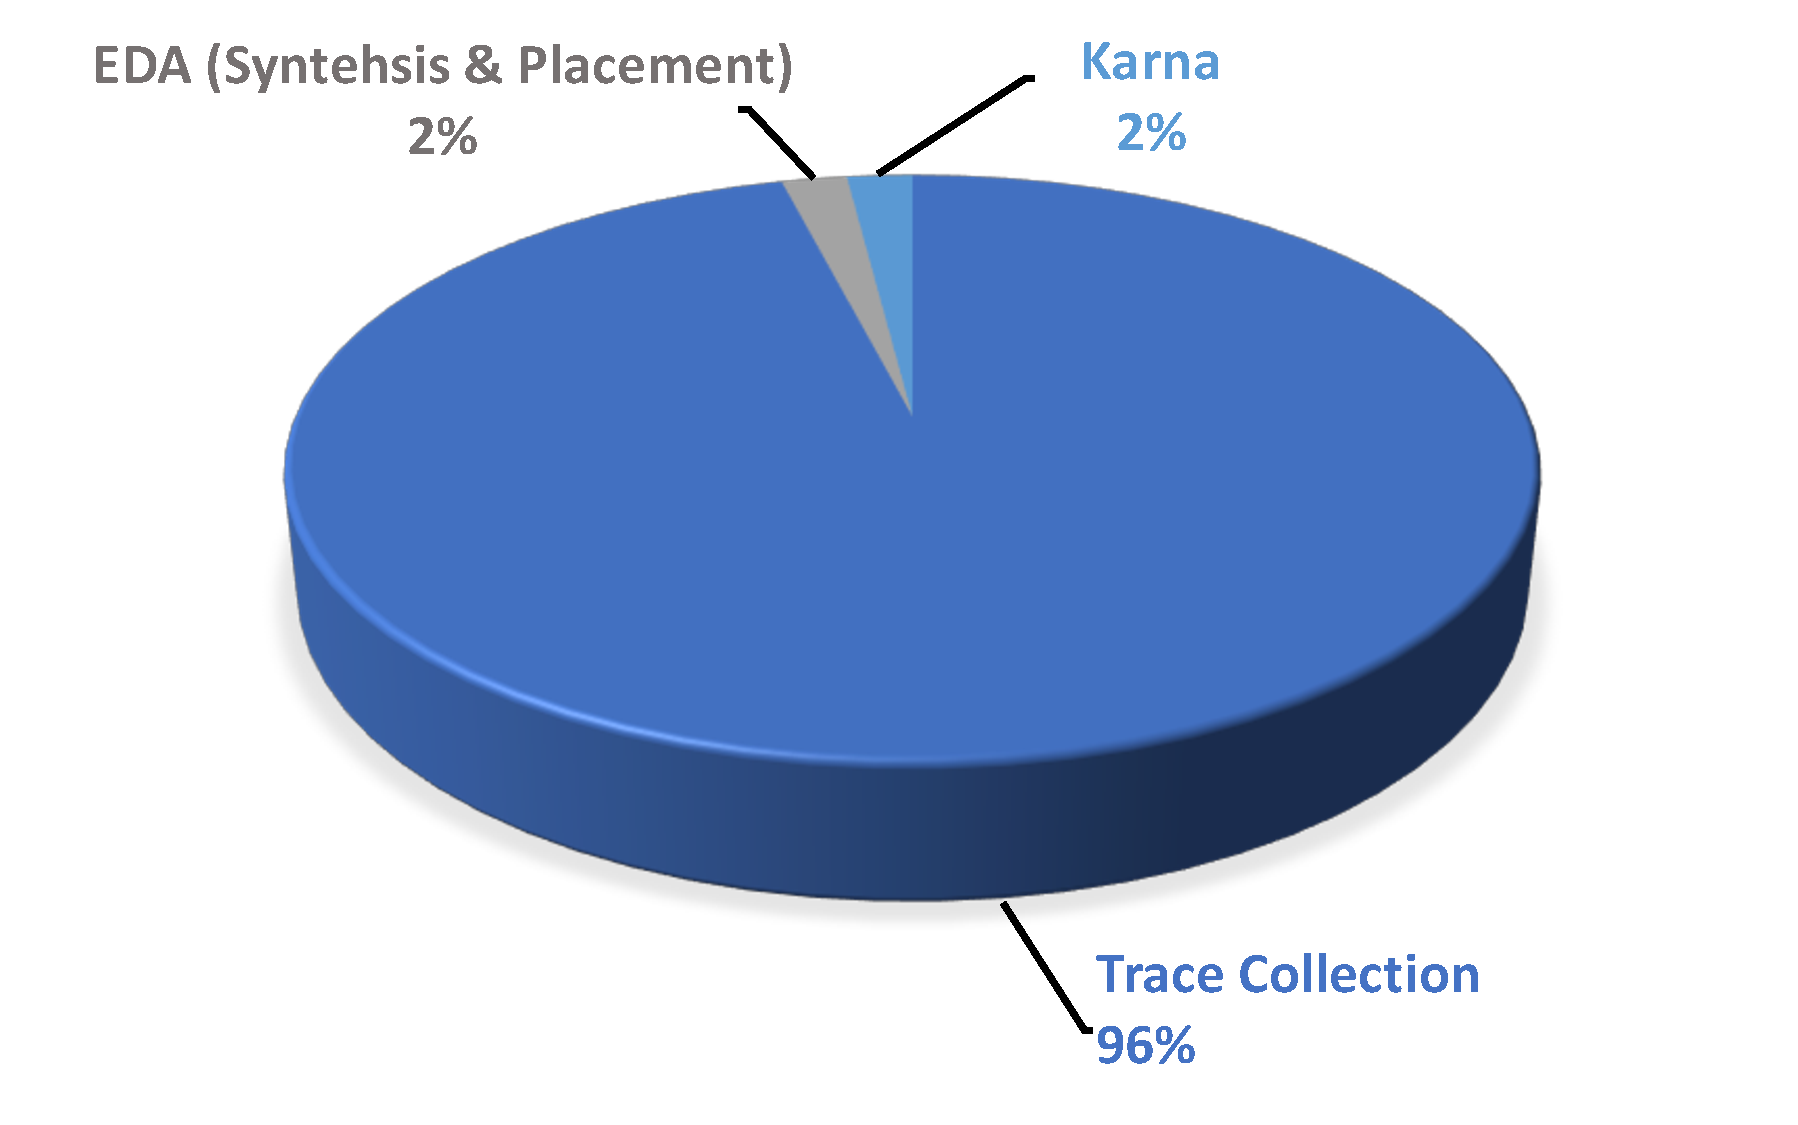
\includegraphics[scale=0.20]{fig/aespie.pdf}
% \caption{Distribution of run time for the AES design}
% \label{fig:aespie}
% \vspace{-15pt}
% \end{figure}


% \begin{figure}[ht!]
% \centering
% 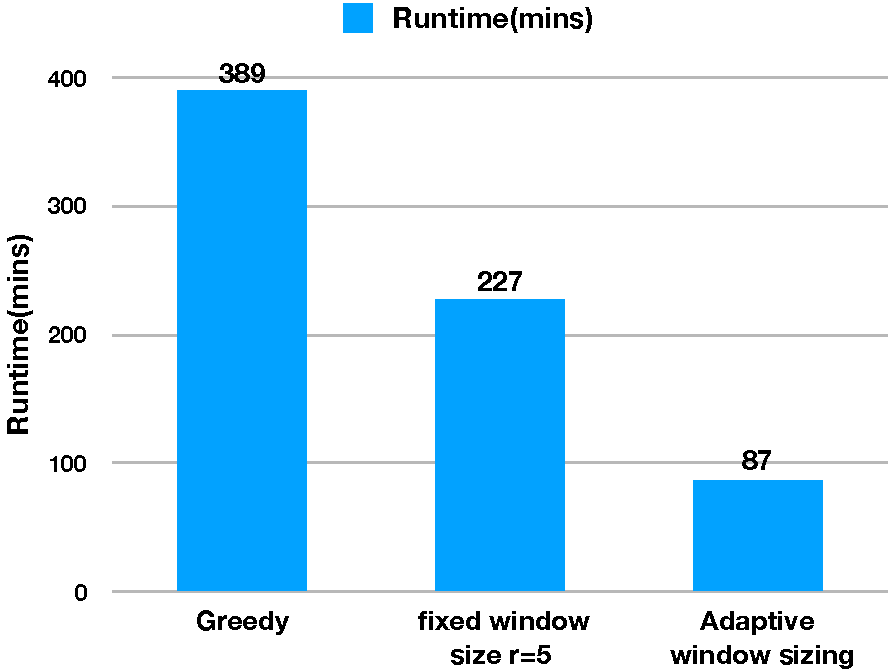
\includegraphics[scale=0.45]{fig/runtime.pdf}
% \caption{Figure showing the variation of runtime with different optimization.}
% \label{fig:tvla}
% \end{figure}





% \section{Discussion}
% \todo[inline]{Convergence of the Karna algorithm with CMOS technology}
% \todo[inline]{The effect of grid size}
% In this section, we discuss the various factors that could affect the convergence of {\sf Karna} algorithm to an optimal solution. 

% \subsection{Number of grids $N_{grids}$} 
 

% \subsection{Standard cell library Technology scaling} 
% The number of $V_{dd}$, $V_{t}$ amd size options influence the overall solution quality and runtime. If the number of options are limited it restricts the ability of the {\sf Karna} algorithm to converge to an optimal solution. However, limiting the number of options will speed up the algoritm as for every gate the number of options that need to be considered are lesser. For example, limiting the number of 
% \subsection{Initial TVLA score}
%It should be noted that the


%\section{Related Work in Pure Exploration Problem}
%\label{tbandit:prevRes}
\begin{figure}[t]
  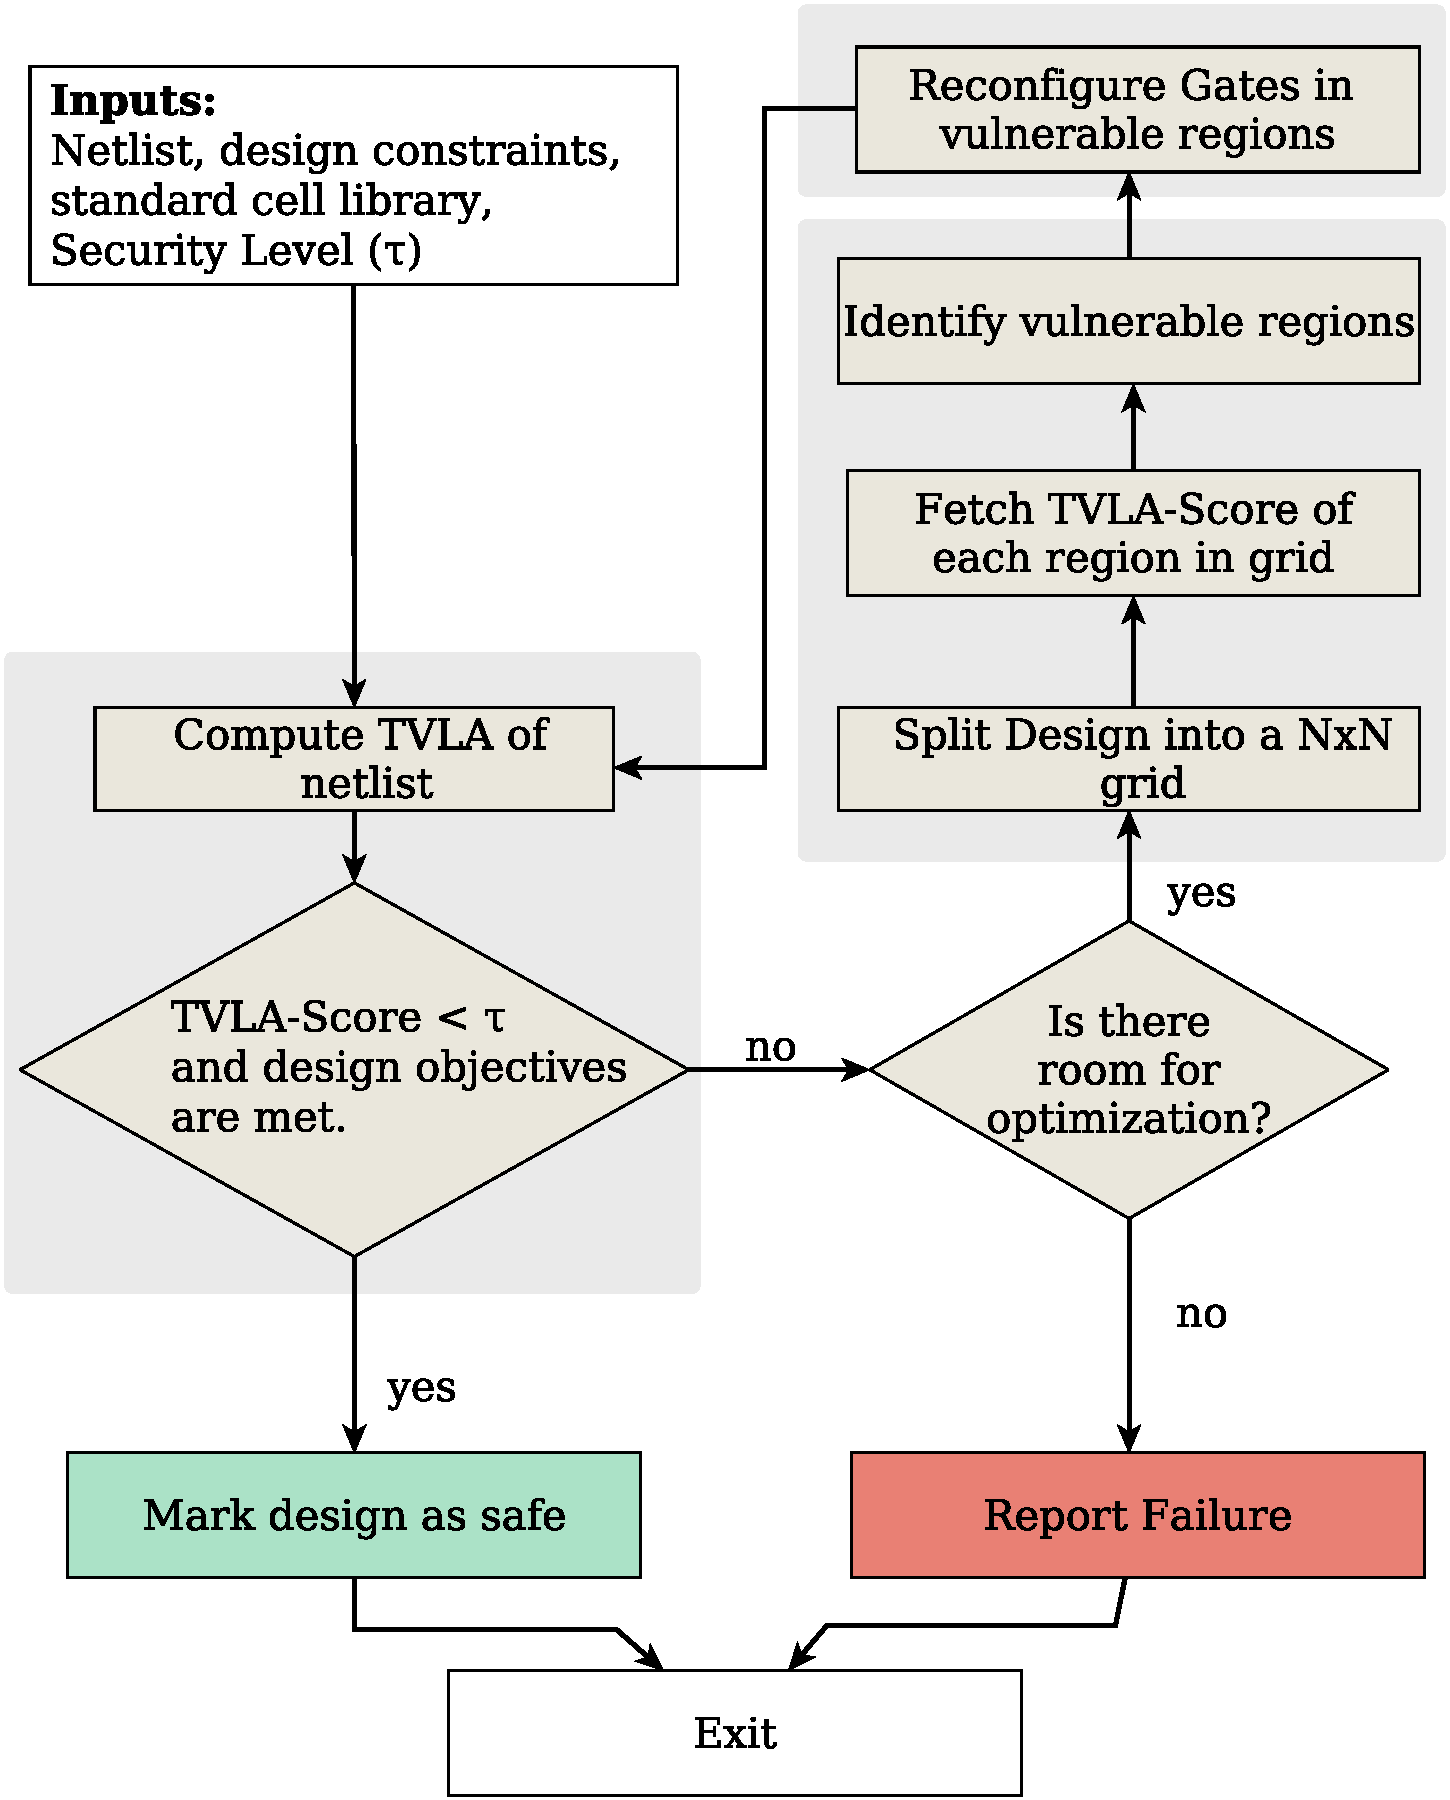
\includegraphics[scale=0.28]{Chapter4/karnamodule}
  \caption{Given a placed netlist, {\sf Karna} tries various configurations for gates present in the standard cell library until the required security $\tau$ is obtained.}
  \label{fig:proposed}
%  \vspace{-15pt}
\end{figure}

\section{{\sf Karna}: AN EDA Module to Reduce Side-Channel Leakage}
\label{sec:proposed}
The {\sf Karna} module (shown in Figure~\ref{fig:proposed}) is executed after the placement stage and before the routing stage in the EDA flow. {\sf Karna} takes as input the placed gate-level netlist represented as a directed acyclic graph $\mathbb C$, where the vertices are the gates and the edges represent interconnects. The various timing, power and area related information, obtained from the standard cell library, is then annotated to each node. Other inputs include $\mathbb P_{g}$, the set of all available choices for every gate type in the standard cell library, the target delay for the design D, and the user-specified security level specified as a desired TVLA score $\tau$.  

{\sf Karna} works in three steps. It first checks if the design meets the desired level of security $\tau$. If $\tau$ is not met, then {\sf Karna} divides the design into an $N \times N$ grid in order to identify the vulnerable regions in the grid. The algorithm then reconfigures the gates in these vulnerable regions until the desired level of security is achieved. We now discuss the implementation of the {\sf Karna} module in further detail. A detailed description is also specified in  Algorithm~\ref{alg:naive}.

{\flushleft \bf Estimating the side-channel security from the netlist.}
{\sf Karna} first estimates if the design meets the user-specified security level by performing the Test Vector Leakage Assessment~\cite{becker:2013} on the gate-level netlist (Line 1 in Algorithm~\ref{alg:naive}). For this, we select the input vectors as per the setup described in~\cite{becker:2013} and perform gate level simulation. The resultant switching information is recorded in a value change dump (VCD) file, that, along with the netlist, is given as an input to the power analysis tool available in the EDA flow. The tool  records the dynamic power traces for each gate in the netlist over a period of time. These traces can be used to compute the TVLA of the entire netlist as well as for specific regions in the netlist. If the TVLA of the design is less than $\tau$, the design passes the check and the algorithm exits successfully, otherwise {\sf Karna} proceeds to identify the vulnerable regions in the design.

{\flushleft \bf Identifying vulnerable regions.}
 {\sf Karna} uses Observation 2 (in Section~\ref{sec:motivation}) that, not all regions of the netlist contribute equally to the side-channel leakage. Hence, in order to reduce  side-channel leakage of a given design, it is sufficient for {\sf Karna}  to identify and optimize vulnerable regions in the netlist. Lines 2 to 12 in Algorithm~\ref{alg:naive} identify the vulnerable regions in the netlist. In order to do this, {\sf Karna} divides the netlist into an $N\times N$ grid and uses the dynamic power traces obtained in the previous step to compute the TVLA for each region $R$ in the grid. If the TVLA score for the region is greater than $\tau$, {\sf Karna} identifies gates that can be optimized by iterating through each gate in the selected region and adding them to a list $\mathbb W$. 
 A gate can be optimized if it meets the following conditions: {\em (i)} it can be replaced with its next low-power configuration {\em i.e.} if it has sufficient positive slack and, {\em (ii)} the gate is not critical. We define a gate to be critical if it cannot undergo any more reconfigurations. If there are no gates available, $\mathbb W = \emptyset$ (Line 13 in Algorithm~\ref{alg:naive}), and the algorithm reports failure and exits, otherwise, {\sf Karna} moves to the next step to reconfigure the vulnerable gates.
 
 




% \begin{framed}
% 1. Start with the flowchart and explain what each step is \\
% 	Explain the TVLA calculation step and how grid level tvla ties to the overall tvla score.\\
%     Explain that the grid can be customized. Explain why you divide into the grid \\
% 2. Explain the leakage optimization algorithm
% 3. Explain the optimization for placement (Need and algorithm)


% \end{framed}




\begin{algorithm}[!t]
%\algsetup{linenosize=\tiny}
  \scriptsize
  %\small
 \LinesNumbered
 \title{The {\sf Karna} algorithm}
 \caption{The {\sf Karna} algorithm}
 \label{alg:naive}
 \KwIn{The design $\mathbb C$ represented as a Directed Acyclic Graph, $\mathbb W$: the set of gates to be reconfigured,
 $\mathbb P_{g}$: the list of all possible configurations for gate g in increasing order of power, D: the delay constraint for the design and $\tau$: the user-specified security level.}
 
%\KwIn{Netlist of the given design C represented as a Directed Acyclic Graph (DAG), initial window size ($r_{init}$), upper bound on window size ($ry_{high}$), set of $V_t$,$V_{dd}$ and size for every gate sorted in increasing order of power, an array A containing the set of gates sorted by the TVLA score. }
\KwOut{Modified $\mathbb C$ so that the overall TVLA score is less than $\tau$.}

\While{$TVLA(\mathbb C) > \tau$}{
  \tcc{Identifying vulnerable regions}

$\mathbb W \leftarrow \emptyset $ \\
Divide the netlist $\mathbb C$ into $N\times N$ regions \\
%$\mathbb R_{regions} \leftarrow$ set of all regions \;
\For{each region $R$ in the  $N \times N$ grid}{
\If{$TVLA(R) > \tau$}{
\For{each gate $g$ in $R$}{
\If{$slack(g) > 0 $ and $g$ is not critical}{
$\mathbb W = \mathbb W \cup \{g\}$
}
}
}
}
\tcc{Reconfiguring vulnerable gates.}

\If{$\mathbb{W} \neq \emptyset$}{
Sort gates in $\mathbb{W}$ based on TVLA scores\\
\For{ each gate $g$ in $\mathbb W$} {
Let $\mathbb P_{g}[j]$ denote the current configuration of gate $g$\\
Let $\mathbb P_{g}[j-1]$ denote the next low power configuration of $g$\\

\If{$j==0$}{Mark $g$ as critical\\ \Continue}

\If{ $slack(P_{g}[j]) \geq delay(\mathbb P_{g}[j-1])-delay(\mathbb P_{g}[j])$  } {
Reconfigure g from $\mathbb P_{g}[j]$ to $\mathbb P_{g}[j-1]$ }
\Else { 
    Mark $g$ as critical\\
    \Continue }
Perform STA on $\mathbb C$ \\
\If{ $delay(\mathbb{C}) > D$}
{undo the reconfiguration done in Line 23\\
Mark $g$ as critical\\
\Continue
}
}
%Detect and fix slew and capacitance violations\;

}
\Else{
Report Failure and exit\;
}
}
%\If{$TVLA(\mathbb C) < \tau$}{
Report Success and exit\\
%Report Failure and quit\;
%}
% \If{No area violations}{
% Report Success and exit\;
 %
%
%
%
%

%%   $r = r_{init}$\; 
%   $state\leftarrow S_{11}$\;
%  $N \leftarrow gate\ count$\;
%   Run STA and compute slack for each gate\;
% % $sensitivity = $\nicefrac{ $\delta leakage \times slack $ }{$\delta delay \times paths$}$ $\;
%  A $\leftarrow$ list of gates whose TVLA score is greater \texttt{-security\_level} and have positive slack, sorted in descending order of sensitivity\; 
% %  \tcc{Note that all gates have slack value $\ge$ 0} 
%   \While{$A.size \ne 0$}  {
%     Take the top $r$ gates ($g_{k_1}, g_{k_2} \ldots g_{k_r}$) in $A$ \;
% %  \tcc{Local validation}
%      For each $g_{k_j}$ ($1 \le j \le r$), check if the increase in delay due to downsizing or upscaling of with its next $V_{dd}$, $V_t$ or $size$
%      version higher to its current version is lesser than its slack. If it is so, replace \;
% %  \tcc{Global validation}
%       Perform a full STA on C \;
%       If delay violation, undo all the reconfigurations done in step 8 \;
%       If $r=1$ mark gate $g$ as critical\;
%       Update the state as per Figure~\ref{fig:state-machine-window-sizing} \;
%       Update the value of $r$ as per Table~\ref{tab:window-sizing-strategy}, for the new value of state \;
%       Mark all the $r$ gates as replaced and remove from A\;
  %  }
 \end{algorithm}
% \begin{table*}[!ht]
%  \begin{minipage}{0.45\textwidth}
%  %\begin{center}
%  \centering

 %\scalebox{0.9}{

%  \begin{tabular}{|c|c|c|p{4cm}|c|}
%  \hline
%  State & $v_{i-1}$ &$v_i$ &Description &$r(i+1)\textsuperscript{*}$ \\
%  \hline
%  $S_{00}$ &0 &0 &Timing violation in the last two iterations& $1$ \\
%  \hline
%  $S_{01}$ &0 &1 &Timing violation in $(i-1)^{th}$ iteration and no timing violation in $i^{th}$ iteration& $(r(i))*2$ \\
%  \hline
%  $S_{10}$ &1 &0 &No timing violation in $(i-1)^{th}$ iteration and timing violation in $i^{th}$ iteration& $r(i) + \alpha$ \\
%  \hline
%  $S_{11}$ &1 &1 &No timing violation in the last two iterations& $r(i)^2$ \\
%  %\scalebox{0.9}{

%  \hline

%  \end{tabular}%}
%  \caption{The 2-bit prediction-based window sizing strategy adopted by {\it HALTimer}}
%  \label{tab:window-sizing-strategy}
%  %\end{center}
%  \end{minipage}\hfill
% %\begin{figure}[!ht]
% \begin{minipage}{0.35\textwidth}
%  \begin{center}
%  \includegraphics[scale=0.4]{fig/state_machine_window_sizing}
%  \captionof{figure}{Transition diagram for the 2-bit prediction scheme adopted by {\it HALTimer}}
%  \label{fig:state-machine-window-sizing}
%  \end{center}
% \end{minipage}
% \end{table*}






%{\sf Karna} works in three steps. First, it checks if the design meets the security requirement. If no, then it identifies the vulnerable regions and reconfigures the gate configurations in these regions. This process continues until the desired level of security is achieved. {\sf Karna} fails when either all gate configurations have been tried out or there is no more room for optimization. In this section we discuss the details of this process.

%\todo[inline]{fig 4. is it "Mark placement as safe" or "Mark netlist as safe"}

%takes as inputs the gate level representation of the design (gate-level netlist), the user specified security level, the standard cell library files, and $N_{grids}$. The parameter $N_{grids}$ specifies the number of grids the netlist must be divided into.  We now describe each steps in detail.
% \begin{figure}[!ht]
%  \centering
%   \includegraphics[scale=0.5]{fig/flow2.pdf}
%   \caption{The proposed flow. }
%   \label{fig:sub4}
% \end{figure}

%{\flushleft \bf Estimating the Side-Channel Security from the Netlist.} 
%For several input test vectors, {\sf Karna} performs a gate level simulation. The resulting switching information, stored in a value change dump (VCD) file, along with the gate-level netlist is given as an input to a power analysis tool, which records the dynamic power traces of each gate in the netlist over a period of time. These traces are then used to compute the TVLA~\cite{becker:2013} for the netlist. 
%If the TVLA score is less than $\tau$ then {\sf Karna} marks the netlist as safe and successfully exits. Otherwise, the next step is invoked which identifies the vulnerable regions in the design, 

%we divide the netlist into grid and use the power trace information to compute the TVLA score for each grid.
%Side-channel leakage of the design can be measured using a metric such as Test Vector Leakage Assessment (TVLA~\cite{becker:2013}). The required security level translates into the permitted TVLA score. If the TVLA score of the design  



%If the leakage from a particular grid is not within the limits specified by the user, the gates belonging to that grid are then reconfigured so as to reduce side-channel leakage. Subsequently, each gate in the vulnerable grid is reconfigured by optimizing one or more of the gate parameters such as supply voltage ($V_{dd}$), threshold voltage ($V_{th}$), load capacitance ($C_{load}$), and gate size. Modifying one or more of these gate-level parameters would impact the other design constraints. Therefore, we also verify that the area, power, and delay constraints are met. These operations are iteratively performed until the TVLA of every vulnerable grid in the design is within acceptable limits.

%The {\sf Karna} module takes as inputs the synthesized netlist which is a gate-level representation of the original design realized as per the design requirements realized at the synthesis step. In order to accurately esitmate the impact on the area constraint, the floorplan information, containting the location of each gate is passed via the def file. The module also takes as inputs the standard cell library which contains the power and delay information for each gate. The {\sf Karna} module lets the user specify the desired by the user by using the \texttt{-security\_level} option. The option specifies the TVLA score that the design is expected to meet. A lower TVLA score implies that the design is expected to meet strict security requirements while a higher score relaxes the security constraint for the design. 

%As mentioned in the previous section, the occurrence of side channel leakage is due to the presence of gates in the chip that perform differently when compared to that of a random input. The first step of the framework is to identify these vulnerable gates. The framework takes as inputs, the synthesized and placed verilog netlist, the floor-plan information and the library file. 

%We first check the post-placed netlist for the presence of side-channel leakage using the TVLA metric described in the Section~\ref{sec:background}.  If the netlist has an acceptable TVLA score, we stop the evaluation else if the netlist has the required TVLA score as specified by the \texttt{security\_level} option. If the design passes the module terminates and we proceed to the next step of the EDA flow. If a design fails to meet the desired level of security we then pass it to the next stage where the {\sf Karna } module identifies the vulnerable gates.


%\item 
% {\flushleft \bf Identifying vulnerable regions in the netlist.} 
%  This step uses the floorplan to divide the netlist into an $N\times N$ grid. {\sf Karna} then computes the TVLA score for each region in the grid using the same power traces estimated in the previous step. This is possible because \todo{fill up} If the TVLA score for a region exceeds the specified security level $\tau$ then that region is marked as unsafe. {\sf Karna} extracts all the gates in these unsafe regions that have a positive slack. The positive slack indicates that the gates can be reconfigured without affecting the delays of the design.  {\sf Karna} sorts these gates based on their TVLA and adds them to a list $\mathbb W$. It then reconfigures gates in the list {$W$}. This reconfiguration is discussed in the  next part of this section.
 
 
{\flushleft \bf Reconfiguring gates in unsafe regions.}
% \begin{itemize}
%     \item How we reconfigure gates such that power, delay, and area are not influenced. 
% \end{itemize}
We leverage Observation 3 (Section~\ref{sec:motivation}) that changing gate parameters has an impact on the overall side-channel leakage. {\sf Karna} optimizes gate parameters such that the overall security of the design improves while the design requirements like area, power, and delay remain unaffected. This reconfiguration is done in Lines 13 to 36 in Algorithm~\ref{alg:naive} by using a list $\mathbb P_{g}$ which contains all the possible configurations for gate $g$, sorted in the increasing order of power.
For each gate in $\mathbb W$, {\sf Karna} attempts to reconfigure it from its current configuration ($\mathbb P_g[j]$) to its next low power equivalent ($\mathbb P_g[j-1]$). However, doing so might compromise the design's delay constraint $D$. Hence, {\sf Karna} performs two validations: {\em (i)} a local validation, by checking if the reconfiguration does not violate the slack of the gate (Line 22) and {\em (ii)} a global validation by performing Static Timing Analysis (STA) for the entire design and checking if the arrival times at the outputs of the design do not violate the overall target delay  of the design $D$ (Line 30). The STA routine also checks for slew and capacitance violations and fixes them. If any of these constraints are violated, {\sf Karna} marks the gate as critical. A gate that is marked as critical is barred from taking part in any subsequent reconfiguration in the algorithm. 
The algorithm continues until the TVLA score drops below  $\tau$. This is a success and the result is a netlist $\mathbb C$, with gates suitably configured to meet the side-channel requirements of the design. The algorithm terminates with a failure if there is no room left for optimization. 


{\flushleft \bf An example with Simon.} 
A bit-serial implementation of the Simon block cipher\footnote{$https://opencores.org/projects/simon\_core$} requires 622 gates using a standard cell 28nm library. We identify the best possible delay of the design at 1.12ns and set it as the target delay $D$   and the desired security level $\tau$ is 4.5. We use 8000 inputs to perform TVLA analysis for the netlist $\mathbb C$, which we represent as a directed acyclic graph. In the first iteration of {\sf Karna}, the TVLA of the design is at 20.799 (Table~\ref{tab:simon}). 130 gates are identified as vulnerable as they belong to regions that have high TVLA ($< 4.5$). These gates are added to $\mathbb W$ as per Lines 4 to 12 in Algortihm~\ref{alg:naive}. The algorithm then attempts to reconfigure these gates as per the steps described in Lines 14 to 36. For the 28nm library used, each gate has 90 possible configurations. {\sf Karna} chooses suitable gates and then checks if the design meets $\tau$ by performing a second TVLA analysis. It can be seen that, after the first iteration, the TVLA of the design decreases to 10.83. This is still greater than $\tau$, which prompts  another iteration. The second iteration finds 102 vulnerable gates, which are  added to $\mathbb W$. Upon reconfiguring the gates {\sf Karna} once again, the TVLA score reduces to 4.48 which is less than $\tau$. The algorithm then exits successfully. 

\begin{table}[t!]
\scriptsize
\caption{Table showing the variation of TVLA, $\mathbb C$, $\mathbb W$, Delay and Power for the Simon cipher implementation in each iteration of Algorithm~\ref{alg:naive}. }
\label{tab:simon}
\centering
\begin{tabular}{|c|c|c|c|}
\hline
\textbf{}                                            & \textbf{\begin{tabular}[c]{@{}c@{}}$1^{st}$\\ Iteration\end{tabular}} & \textbf{\begin{tabular}[c]{@{}c@{}}$2^{nd}$\\ Iteration\end{tabular}} & \textbf{\begin{tabular}[c]{@{}c@{}}$3^{rd}$\\ Iteration\end{tabular}} \\ \hline
\begin{tabular}[c]{@{}c@{}}Delay\\ (ns)\end{tabular} & 1.12                                                                     & 1.12                                                             & 1.12                                                             \\ \hline
Power (uW)                                           & 3.70                                                                     & 2.61                                                             & 0.16                                                             \\ \hline
TVLA                                                 & 20.799                                                                   & 10.83                                                            & 4.48                                                             \\ \hline
$\mathbb C$ & \multicolumn{3}{|c|}{622}  \\ \hline
$\tau$ & 4.5 & 4.5 & 4.5 \\ 
\hline
$\mathbb W$ &       130 & 102 & 0 \\ \hline

\end{tabular}
\vspace{-10pt}
\end{table}

{\flushleft \bf Impact of {\sf Karna} on the other design requirements.}
{\sf Karna}, by design, does not violate the power and delay constraints. While the delay constraints are verified at multiple instances in the Algorithm~\ref{alg:naive} (Line 22 and Line 30), the power constraint is inherently met. This is because, {\sf Karna} attempts to replace each gate with its low power equivalents. Thus, the overall power consumption of the design will not increase.

While {\sf Karna} increases the area utilization of the device, it is unlikely to increase the  device size. The reason being, {\sf Karna} never adds any extra gates to the design but only reconfigures a targeted subset of the gates in the entire design. 
Not all the reconfigurations of these gates have an impact on the size. Further, the overall area would only increase if the gates lying at the periphery undergo an increase in size. There is low likelihood of this happening.


{\flushleft \bf Analysis of {\sf Karna}. }
We evaluate {\sf Karna} with respect to success and runtime.

{\flushleft \em Success Analysis.}
The success of {\sf Karna} depends on the value of $\tau$, the target delay of the design $D$, and the number of configurations available for each gate $|\mathbb P_g|$. A high value of $D$ implies that the slack at each gate will be high, thus, fewer gates will be marked critical. Consequently the number of gates taking part in the optimization process increases. Similarly, larger number of configurations available for a gate, will increase the chances that {\sf Karna} will find a gate which can achieve the desired security. A lower value of $\tau$ on the other hand, increases the effort that {\sf Karna} has to put in to achieve  security requirements. This may lead to an infeasible solution. 

\begin{figure}[t!]
\centering
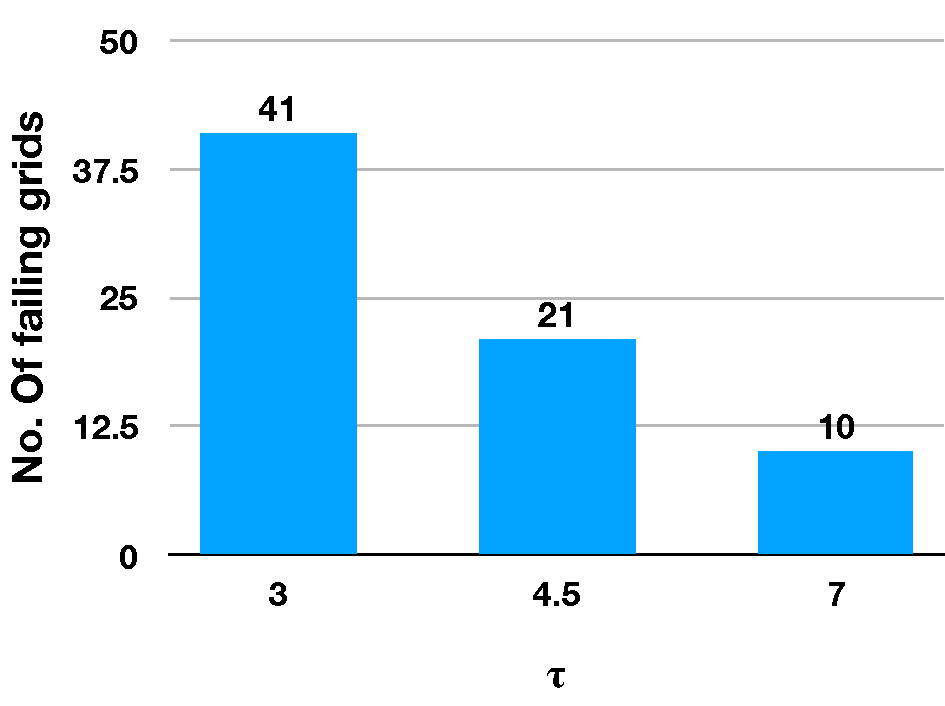
\includegraphics[scale=0.35]{Chapter4/fig/tvla.pdf}
\caption{Figure showing the number of failing regions with respect to $\tau$. It can be seen that it varies inversely with $\tau$.}
\label{fig:runtime}
%\vspace{-10pt}
\end{figure}

{\flushleft \em Runtime Analysis.} Each iteration of the {\em while} loop requires one trace collection step  to compute the TVLA in Line 1 and Line 5 of the algorithm. This trace collection takes up major portion of the run time. Besides this, the run time for the rest of {\sf Karna} is considerably small and is influenced mainly by the size of $\mathbb W$, the number of regions, and the security parameter $\tau$. 
A large value of the target delay $D$ implies that a large number of gates get added to $\mathbb W$ in Line 7 of Algorithm~\ref{alg:naive}. Similarly, a small value of $\tau$ indicates more number of regions failing (as seen in Figure~\ref{fig:runtime}), which in turn increases the size of $\mathbb W$. 
A  large value of the grid size will increase the run time as the number of regions that need to be checked in Line 4-5 of Algorithm~\ref{alg:naive} increases. 

Other factors that influence the run time are the number of local and global validations performed in Algorithm~\ref{alg:naive}. For each global validation, an STA call is made in Line 29 of Algorithm~\ref{alg:naive}. A full blown STA would have a run time complexity of $\mathcal{O} ( G^{2})$ where $G$ is the total number of gates in the design. In order to reduce the rum time, incremental Static Timing Analysis models such as the one used in~\cite{hu:12} or adaptive lazy timing analysis techniques like~\cite{MLTimer} can be employed. 

%\vspace{-3pt}
%The size of $\mathbb W$ also determines the termination 






%\todo{Factors influencing solution quality, runtime and factors influencing termination}
%which would cause only a minimal increase in the area. From our experiments, we observed that while the overall area remained constant, the area utilization increased.


%However, reconfiguring each gate with its low power equivalent will increase the delay of that particular gate. {\sf Karna} ensures that the reconfiguration doesn't violate the delay constraint by first checking if the gate has sufficient positive slack to undergo the reconfiguration (Line 22) and also perform Static Timing Analaysis on the design to ensure that the arrival time and required time constraints at all end-points are met (Line 30). It should be noted that though this timing analysis is a costly procedure, it ensures that the delay constraints are not violated. 

%The next configuration for each gate is chosen from the list P which consists of all the possible configurations sorted in increasing order. The algorithm traverses this list from right to left iteratively 
% We make use of Observation 3  (Section~\ref{sec:motivation}), i.e.,
% tuning gate parameters such as $V_{dd}$, $V_t$, and size can influence the side-channel leakage from the gate.
% In this step, we focus on optimizing the gate parameters such that the overall security of the design improves while the design parameters like area, power and delay remain unaffected.
% We use the Algorithm~\ref{alg:naive} for optimizing these gate parameters. The algorithm takes as input the synthesized netlist, the target frequency $F$ and, a standard cell library containing multiple cells with different $V_{dd}$, different threshold voltages $V_t$ and sizes for every gate. The netlist is represented as a Directed Acyclic Graph where the gates are represented by the nodes in the graph and the edges represent interconnects. The set of gates belonging to the vulnerable grids are stored in an array A.

% The algorithm works as follows, the gates are sorted in descending order based on their TVLA scores. The gate with the highest score i.e, the gates that are the most vulnerable in the design are the beginning of the list and the gates that are least vulnerable are the end. The algorithm then iteratively tries to optimize the $V_{dd}$, $V_{t}$ and size of each gate. The algorithm then checks for delay violations and commits the change if the proposed optimization doesn't violate the available delay budget of the gate. We then run a timing analysis to check if the proposed change causes any timing violations and undo the change if there are any such violations.

% It should be noted that this method is expensive in terms of runtime as the timing analysis procedure needs to be run for each and every gate in the array A. In order to speedup the optimization process we use the procedure reported in~\cite{MLtimer}. We define the set of gates that can be replaced in each iteration as the gate\_reconfiguration\_window $r$. Figure~\ref{fig:state-machine-window-sizing} and the value of $r$ at the end of every timing update is given in Table~\ref{tab:window-sizing-strategy}. It can be observed from this transition diagram that $state$ in timing update $i$ can be represented as $S_{v_{i-1}},v_i$, where $v_{i-1}$ and $v_i$ are binary digits that denote the stats of $(i-1)^{th}$ and $i^{th}$ timing updates respectively. A status of $v=0$ indicates a timing violation while a $1$ denotes a successful timing update. 
% We initialize $r$ to 2 and incrementally update the value of $r$ depending on the $state$ of the timing update. We limit the maximum value of $r$ to $\frac{N}{2}$, where $N$ stands for the total number of gates in the design. For example, if there is a timing violation in iterations $(i-1)$ and $i$ then the value of $r$ is set to 1 and the $state$ is set to 00, and only one gate is updated in the next iteration $(i+1)$, and if in the $(i+1)^{th}$ iteration there is no timing violation then the $state$ variable is updated to 01 and the value of $r$ is set to $r(i)*2$ ( 2 in this case as only one gate was replaced in the $i^{th}$ iterataion) and $r(i)*2$ gates are analyzed in the current iteration. Thus, the algorithm adaptively varies the window size depending on the $state$ variable.
% We sum up each iteration of the algorithm in the following steps.
% \begin{itemize}
 

% \item For each gate in the list A sort the gates based on the TVLA scores.

% \item For the first $r$ choices of A\; perform the following steps\;
% 	\begin{itemize}
%       \item if the gate has sufficient positive slack, we then replace the gate with the next configuration.
%     \end{itemize}

% \item We then check for any timing violations by running Static Timing Analysis. 

% \item If there is any delay violation, undo all reconfigurations.
% \begin{itemize}
% \item if $r$ is 1, then mark the corresponding gate as critical so that it cannot participate in any further timing optimizations.
% \item Update state and compute the new value of $r$.
% \end{itemize}
% \item  If timing evaluation is successful
% \begin{itemize}
% 	\item Run TVLA estimation, sort the gates based on updated TVLA values.
%     \item Update $state$ and compute the new value of $r$.
%     \item if value of $r$ is greater than A, the we resize $r$ to $\frac{A.size}{2}$.
% \end{itemize}

% \end{itemize}

%\item
%At the end of each iteration, {\sf Karna} checks the netlist for slew and capacitance violations. We incrementally upsize each gate in order to fix them. %Figure~\ref{fig:karna}
%shows the working of the {\sf Karna} module. 
%\end{itemize}
 
 
%Figure~\ref{fig:aesopt} showed that not all regions in the chip have a uniform TVLA value. In this step, we identify and optimize the gates in such vulnerable regions of the netlist. %It can be seen that for any given input, the amount of switching activity is different for different areas of the design. The side-channel leakage could be due to some areas of the design switching at a different rate for a specific input when compared to a random input.%Hence, in order to reduce the side-channel leakage  the gates belonging to these vulnerable areas need to be optimized. 
%In this step, we identify and optimize the gates in such vulnerable regions of the netlist.


 
 
 
 
% {\sf Karna} tries to achieve security without violating the design requirements. However, as mentioned earlier choosing gate configurations that favour security might violate the delay or area constraint. Hence, {\sf Karna} tries to balance between these two requirements.  It should be noted that the size of a region determines the nature of optimizations performed by {\sf Karna}. For example, consider the scenario where the value of $N$ is set such that there is only one gate per region. In this scenario {\sf Karna} would be able to identify uniquely the set of gates violating the secuirty constraints and change their configuration. This might cause the algorithm to select choices that are locally optimal i.e, they improve the overall security of the design but 
 
 
 
% While a high value of $N$ aggressively optimizes the design for security even at the cost of area and delay, a very low value would perform a lazy security optimization. For instance, when $N_{grids}=1$, the entire design is considered as a whole during the optimization process. This means that the algorithm might select gates that 
 
 
 %assessed for TVLA compliance. If it fails the TVLA test, all the gates belonging to the design are added to the working set of gates that needs to be optimized. This may lead to performance issues for designs that have a large number of gates. On the contrary, when $N_{grids}$ is equal to the number of gates in the design, each gate is checked for TVLA compliance and only the vulnerable gates are optimized. While this approach reduces the number of gates in the working set, this is also sub-optimal since the TVLA test has to be run for every gate in the design. More importantly, the algorithm may disregard placement dependencies between grids (i.e., delay and area budget of the design as a whole) since each grid is optimized in an isolated manner. Therefore, there is a need to select an optimal value of $N_{grids}$.

%A very high value of $N_{grids}$ will perform a fine-grained security analysis on the design while a low value of $N_{grids}$ will perform a coarse-grained analysis. For instance, setting $N_{grids}$ to the number of gates in the design will calculate the TVLA score for each gate in the netlist and identify if it is vulnerable, while a value of 1 will analyze the entire design as a whole and add all the gates to the vulnerable list. Thus the value of $N_{grids}$, much like the \texttt{-security\_level} option lets the designer specify the level of security expected from the design. A high value of $N_{grids}$ coupled together with a very low TVLA threshold would set extremely high security constraints on the design. Once the netlist is divided, the TVLA score is then calculated for each grid in the netlist. All the grids that do not comply with the TVLA score specified in the \texttt{-security\_level} option are marked as \textbf{unsafe} and the gates that belong to these grids are added to a working set. We then carefully tune the gate parameters of all the gates in this set in the next step, in order to improve the security of the design.


%{\flushleft \bf Reconfiguring the unsafe areas}


%\section{TBP Connection to Pure Exploration Problem}
%\label{tbandit:connection}
\section{Related Work}
\label{sec:related}
% \todo[inline]{
% Organize related work as follows:

% Side-channel countermeasures can be applied at either the algorithm level, system level, or device level.

% Algorithm level countermeasures include masking, threshold implementations, rekeying.

% System level countermeasures include all the power noise aspects.

% Ours is most close to 
% Device level include WDDL, SABL, etc.
% }
%\subsection{Related Work:}
Side-channel attack countermeasures can be categorized as algorithmic, physical, or system-level. Algorithmic countermeasures insert additional operations that mask~\cite{akkar:2001} or split~\cite{Bilgin:2014} the sensitive computation. System-level countermeasures, such as~\cite{Wang:2013,tokunaga:2009,singh:2015,mathew:2018}, use the device's power supply to  normalize or randomize the overall power consumption. Physical countermeasures like ~\cite{Kim2017,Tiri:2004} use custom gates that consume power independent of the gate's switching. While  algorithmic and system-level countermeasures require additional circuitry, {physical countermeasures} use custom logic design methodologies to tackle the leakage. {\sf Karna} on the other hand requires no additional circuitry nor custom logic therefore has much lower overheads.  
{\sf Karna} in principle, is similar to ~\cite{Tiri:2004}, where side-channel resistant gates are realized by combining multiple standard cell gates. However, the size of each compound gate is considerably larger, resulting in a 4$\times$ increase in area. {\sf Karna} on the other hand, simply reconfigures gates in the design. Thus the area is not affected. Gate reconfigurations during the EDA flow have been used in the past to ensure low-power design~\cite{hu:12,flach:2014} and high-performance~\cite{ozdal:2012}. To the best of our knowledge, {\sf Karna} is the first to use gate reconfiguration to address side-channel leakage.

%The EDA flow is responsible for translating the design specified in a high level language like Verilog into actual hardware. Gate sizing algorithms attempt to select the best possible configuration of the gate such that the objectives at the corresponding stage are achieved. Works like~\cite{hu:12, ozdal:2012,reimann:13,li:2012,flach:2014} propose a sizing algorithm that focuses on varying the threshold voltage $V_t$ and the size of the gate in order to reduce the power consumption of the design.  While~\cite{hu:12,reimann:13} use heuristics like simulated annealing to reconfigure the gates, \cite{ozdal:2012,li:2012,flach:2014} use analytical techniques to solve the problem. However, none of the prior works attempt to leverage the EDA flow in order to counter the power side-channel. To the best of our knowledge ours is the first work try and use the gate sizing techniques to mitigate power side-channels.
%\vspace{-3pt}
\section{Conclusion and Future Work}
\label{sec:conclusion}
{\sf Karna} demonstrates that side-channel security of a device can be improved by reconfiguring the vulnerable gates in the design. This allows security constraints to be elegantly integrated into any EDA flow permitting designers to achieve design security with minimal overheads. {\sf Karna} works on a post placed netlist and is tested successfully on three popular cipher implementations and meets the desired security level (4.5) with minimal impact on area,power and delay. Our current results show drastic increase in EDA design time, mainly due to power trace collection needed for TVLA computation. In the future we plan to optimize this step by parallelization and with better side-channel metrics. Another direction of work is to evaluate {\sf Karna} to address other side-channel attacks like fault injection and timing. 


%In our proposed flow, we investigate the impact of various design optimizations on the security of the device using the metric proposed in~\cite{becker:2013}. We identify potential regions in the netlist that are vulnerable and use a gate sizing scheme to reconfigure the $V_{dd}$, $V_t$ and $size$ values in the netlist such that the overall t-score of the netlist falls under the prescribed limits. 



% \begin{itemize}
% \item \textbf{Prior Survey}: \cite{Yang2017}:Hardware Designs for Security in Ultra-Low-Power IoT Systems: An Overview and Survey; \cite{Duarte2009}: A note on the security of M ST 3; \cite{Diehl2018}: Comparing the cost of protecting selected lightweight block ciphers against differential power analysis in low-cost FPGAs; 

% \item \textbf{Attacks}: \cite{Moradi2014}:Side channel attack using static power;\cite{Alioto2010}: Leakage Power attacks; \cite{Wei2018}: I Know What You See: Power Side-Channel Attack on Convolutional Neural Network Accelerators
% \cite{Singh2017}: Improved power side channel attack resistance of a 128-bit AES engine with random fast voltage dithering.
% \item \textbf{Analysis on SideChannel Attacks}: \cite{Moos}:Static Power Side-Channel Analysis of a Threshold Implementation Prototype Chip;  \cite{Reparaz2017}: Dude, is my code constant time?; \cite{Goodwill2011}: A Testing Methodology for Side-Channel Resistance Validation;  \cite{Roy2015}:From theory to practice of private circuit: A cautionary note (This paper talks about leakage detection tests, more of an analysis than a metric, could be a section after discussing attacks); \cite{Moosa}: Glitch-Resistant Masking Revisited or Why Proofs in the Robust Probing Model are Needed; \cite{Zoni2018}: A Comprehensive Side-Channel Information Leakage Analysis of an In-Order RISC CPU Microarchitecture; \cite{Brier2004}: Correlation Power Analysis with a Leakage Model; \cite{Bache2018}: Confident Leakage Assessment -A Side-Channel Evaluation Framework based on Confidence Intervals

% \item \textbf{Metric}: \cite{Veyrat-charvillon2013}: Certify leakage of a chip; \cite{Schneider2016}:Leakage assessment methodology; \cite{Federal2017}: A Platform to Evaluate the Fault Sensitivity of Superscalar Processors; \cite{Standaert2017}: How (not) to Use Welch's T-test in Side-Channel Security Evaluations; \cite{Corre}: Micro-Architectural Power Simulator for Leakage Assessment of Cryptographic Software on ARM Cortex-M3 Processors
% \cite{Mather}: Does My Device Leak Information? An a priori Statistical Power Analysis of Leakage Detection Tests; \cite{Zhang}: Towards Sound and Optimal Leakage Detection Procedure; \cite{Reparaz}:Fast Leakage Assessment; \cite{Sadhukhan2017}: An Evaluation of Lightweight Block Ciphers for Resource-Constrained Applications: Area, Performance, and Security; \cite{Barenghi2018}: Side-channel security of superscalar CPUs Evaluating the Impact of Micro-architectural Features;

% \item \textbf{Model Using some metric to avoid attacks}: \cite{Leiserson2014}: Gate-Level Masking under a Path-Based Leakage Metric; 

% \item \textbf{Models to provide security against attacks}: \cite{DeCnudde2016}: Masking AES with $d + 1$ shares in hardware; \cite{Ghoshal2017}: Several masked implementations of the boyar-peralta AES S-Box; \cite{DeCnudde2017}: Securing the PRESENT Block Cipher Against Combined Side-Channel Analysis and Fault Attacks; \cite{Kar2018}: Reducing Power Side-Channel Information Leakage of AES Engines Using Fully Integrated Inductive Voltage Regulator; \cite{Wegener}: A First-Order SCA Resistant AES without Fresh Randomness; \cite{DeCnudde2017}: Securing the PRESENT Block Cipher Against Combined Side-Channel Analysis and Fault Attacks; \cite{Seuschek2017}: Side-channel leakage aware instruction scheduling;  \cite{Kim2017}: STBC: Side Channel Attack Tolerant Balanced Circuit with Reduced Propagation Delay; \cite{Patranabis2016}: Shuffling across rounds: A lightweight strategy to counter side-channel attacks ; \cite{Judd2016}: Proteus; \cite{Gross2018}: Generic Low-Latency Masking in Hardware;\cite{Ghoshal2018}: Lightweight and Side-channel Secure 4 × 4 S-Boxes from 
% Cellular Automata Rules; \cite{Agosta2015}:The MEET Approach: Securing Cryptographic Embedded Software Against Side Channel Attacks; 

% \item \textbf{Miscellaneous}: \cite{Levi2017}CPA Secured Data-Dependent Delay- Assignment Methodology;  \cite{Profile2014}: Optimum Leakage Recovery using Synopsys Primetime ECO Leakage Recovery Flow; \cite{Gross2018a}: Generic Low-Latency Masking in Hardware; \cite{Gierlichs2008}: Mutual Information Analysis; \cite{Peng2018}: Framework for efficient SCA resistance verification of IoT devices

% \end{itemize}




% \section{Related Work in Thresholding Bandits}
% \label{tbandit:prevResAPT}
% \input{Chapter4/prevResAPT}


\section{Summary}
%\label{tbandit:conc}
%\input{Chapter4/conc}


%%%%%%%%%%%%%%%%%%%%%%%%%%%%%%%%%%%%%%%%%%%%%%%%%%%%%%%%%%%%%%%




%%%%%%%%%%%%%%%%%%%%%%%%%%%%%%%%%%%%%%%%%%%%%%%%%%%%%%%%%%%%%%%
\clearemptydoublepage
% \chapter{Augmented UCB for Thresholding Bandit Problem}
% \label{chap:tbandit2}

% \section{Introduction}
% \label{tbandit:intro2}
% One of the significant moments that has shaped human history was the invention of the computer. What essentially started out as an attempt to replace and replicate simple arithmetic functions now surrounds us on a day-to-day basis taking care of our transport, health, finance and ingratiating itself into our daily lives more and more. 

This evolution has largely been made possible due to the invention of the transistor by Bell & Schokley in 1951 which caused computers to go from the size of an airplane hangar to tiny microscopic devices.  The invention of the transistors enabled chip designers to meet the ever increasing user requirements by halving the size of the transistors and thereby doubling the number of transistors that could be packed into the same area. This phenomenon also dubbed as Moore’s law has enabled chip designers meet the exponentially increasing functionality requirements.

In addition to increasing functionality, digital devices are also expected to meet additional constraints which can be enumerated using the tuple {Power, Area and Delay}. Depending on the platform in which it gets deployed, the chip designer might have to optimize the same design to meet  two orthogonal constraints. For example, when building a server, the processor is expected to be fast while the power and area requirements are relaxed but on the other hand if the same processor is to be used on a IoT device, the designer might have to optimise the design for low power, smaller area while the device might not be expected to perform at the same speed as the server. **{ Can we rewrite it with a better example?}

We now discuss the three key objectives that a given digital design is expected to meet. 
\begin{enumerate}
    \item \textbf{Delay} With each passing generation 
\end{enumerate}





%Computers have evolved from being simple calculators to devices that can perform complex operations that are employed in various aspects of our day-to-day lives.  
%This evolution has been 

%For the last 70 years, chip designers have been able to meet this expectation by leveraging Moore's law and adding more transistors.  

%Today digital devices can be broadly classified into three different classes \begin{enumerate}
 %   \item Embedded devices: These devices are expected to interact with various aspects of a user's environment such as temperature, motion etc. and make decisions on the fly. The emergence of Internet of Things as a popular networking paradigm in the last 3 years has led to an increase in the demand for such devices. These class of devices typically application specific and perform either "send and send" or lightweight computation at the
%\end{enumerate}

%In this evolution, the expectations of the end-user from each generation has been increasing. While initial generations were expected to merely speed-up arithmetic operations, the development of commercial compute devices starting with Intel's 4004 processor has led to these devices perform complex mathematical functions at a faster rate, on a smaller device by using a little energy as possible. 












% In today's world, artificial intelligence has proved to be a game-changer in designing agents that interact with an evolving environment and make decisions on the fly. The main goal of artificial intelligence is to design artificial agents that make dynamic decisions in an evolving environment. In pursuit of these, the agent can be thought of as making a series of sequential decisions by interacting with the dynamic environment which provides it with some sort of feedback after every decision which the agent incorporates into its decision-making strategy to formulate the next decision to be made. A large number of problems in science and engineering, robotics and game playing, resource management, financial portfolio management, medical treatment design, ad placement, website optimization and packet routing can be modeled as sequential decision-making under uncertainty. Many of these real-world interesting
% sequential decision-making problems can be formulated as reinforcement learning (RL) problems (\citep{bertsekas1996neuro}, \citep{sutton1998reinforcement}). In an RL problem, an agent interacts with a dynamic, stochastic, and unknown environment, with the goal of finding an action-selection strategy or policy that optimizes some long-term performance measure. Every time when the agent interacts with the environment it receives a signal/reward from the environment based on which it modifies its policy. The agent learns to optimize the choice of actions over several time steps which is learned from the sequences of data that it receives from the environment. This is the crux of online sequential learning. 

%     This is in contrast to supervised learning methods that deal with labeled data which are independently and identically distributed (i.i.d.) samples from the considered domain and train some classifier on the entire training dataset to learn the pattern of this distribution to predict the labels of future samples (test dataset) with the assumption that it is sampled from the same domain. In contrast to this, an RL agent learns from the samples that are collected from the trajectories generated by its sequential interaction with the system. For an RL agent, the trajectory consists of a series of sequential interactions whereby it transitions from one state to another following some dynamics intrinsic to the environment while collecting the reward till some stopping condition is reached. This is known as an episode. Here, for an action $i_t$ taken by the agent at the $t$-th timestep, the agent transitions from its current state denoted by $S_{i,t}$ to state $S_{i,t+1}$ and observes the reward $X_{i,t}$. An illustrative image depicting the reinforcement learning scenario is shown in Figure \ref{fig:rl}.

% \begin{figure}[!th]
% \includegraphics[scale=0.45]{Chapter1/img/RL1.png}
% \caption{Reinforcement Learning}
% \label{fig:rl}
% \end{figure}


    
    
% %To express an RL problem more formally, we have to define the idea of Markov Decision Process (MDP) which consists of states, actions, transition probabilities, and rewards which in turn helps in deciding the strategy to be followed by the agent. 

% %An MDP consists of states



% \section{Our Contributions}
% \label{tbandit:contribution}
% The main contributions of the thesis are as follows:-
\begin{enumerate}
\item We propose the MLTimer alogrithm that uses gate-sizing for reducing the leakage power consumption of a digital design. We propose a smart one-pass tool that can leverage the right optimization technique at the appropriate stage of the flow thereby improving design productivity. A key observation reported in MLTimer is that there exists significant correlation between the timing slacks of gates in the current iteration to the gate replacements in successive iterations. MLTimer leverages this observation to reduce the number of STA runs thereby reducing the overall time taken for optimization.

\item We propose the Karna algorithm which uses gate-sizing for reducing the information leakage via the power side-channel of a digital design. We show that each region in a given design leaks information differently. Thus, it is sufficient to optimize gates in the highly sensitive regions to reduce information leakage. Karna leverages this observation and optimizes gates in these sensitive regions to reduce the power side-channel vulnerability. 

%\item We proposed a general framework of bandit algorithms that combines change-point detection algorithm with aggregation of expert strategies in order to define efficient pulling strategies in the context of the piecewise stochastic distributions. The algorithms that we proposed for the piecewise stochastic setting are actively adaptive algorithms which perform very similarly to the oracle algorithm which has access to the changepoints and suffers no additional delay in adapting to the changing environment. 
\end{enumerate}
 


% \section{Augmented-UCB Algorithm}
% \label{tbandit:algorithm}
% \input{Chapter5/algo}


% \section{Theoretical Results}
% \label{tbandit:results}
% \section{Results}
\label{sec:results}
% \begin{table}[!ht]
% \centering
% \caption{My caption}
% \label{my-label}
% \begin{tabular}{|p{1.2cm}|l|l|l|l|l|l|}
% \hline
% \multirow{2}{*}{\begin{tabular}[c]{@{}c@{}}Feature \\ Name\end{tabular}} & \multicolumn{2}{c}{Vt Classifier}                                       & \multicolumn{4}{|c|}{Size classifier}                                                                                                   \\ \cline{2-7} 
%                                                                          & \multicolumn{1}{c|}{1} & \multicolumn{1}{c|}{2} & \multicolumn{1}{c|}{ 1} & \multicolumn{1}{c|}{ 2} & \multicolumn{1}{c|}{3} & \multicolumn{1}{c|}{4} \\ \hline
% Sub-circuit                                                              & \multicolumn{1}{l|}{}        &                               &                               &                               &                              &                              \\ \hline
% Gate Type                                                                & \multicolumn{1}{l|}{}        &                               &                               &                               &                              &                              \\ \hline
% LNS                                                  & \multicolumn{1}{l|}{}        &                               &                               &                               &                              &                              \\ \hline
% \#Fanins                                                                 & \multicolumn{1}{l|}{}        &                               &                               &                               &                              &                              \\ \hline
% \#Fanouts                                                                & \multicolumn{1}{l|}{}        &                               &                               &                               &                              &                              \\ \hline
% \begin{tabular}[c]{@{}l@{}}\#Negative \\ Slack Paths\end{tabular}                                          & \multicolumn{1}{l|}{}        &                               &                               &                               &                              &                              \\ \hline
% Slack                                                                    & \multicolumn{1}{l|}{}        &                               &                               &                               &                              &                              \\ \hline
% \end{tabular}
% \end{table}
% \begin{table*}[!ht]
% \centering
% \caption{result3}
% \label{results3}
% \begin{tabular}{|l|c|l|l|l|l|l|l|l|l|l|l|}
% \hline
% \multicolumn{1}{|c|}{\begin{tabular}[c]{@{}c@{}}Benchmark \\  Name\end{tabular}} & \begin{tabular}[c]{@{}c@{}}Number \\ Of gates\end{tabular} & \multicolumn{1}{c|}{\begin{tabular}[c]{@{}c@{}}Target \\ Delay\end{tabular}} & \begin{tabular}[c]{@{}l@{}}Inital \\ Delay\end{tabular} & \multicolumn{2}{c|}{SVM}                                         & \multicolumn{2}{c|}{Final}                                      & \multicolumn{2}{c|}{Igor Markov}                               & \multicolumn{2}{c|}{Flach}                                     \\ \hline
% \multicolumn{1}{|c|}{}                                                           &                                                            & \multicolumn{1}{c|}{}                                                        & \multicolumn{1}{c|}{}                                   & \multicolumn{1}{c|}{Delay (ns)} & \multicolumn{1}{c|}{Power (W)} & \multicolumn{1}{c|}{Delay (ns)} & \multicolumn{1}{c|}{Power(W)} & \multicolumn{1}{c|}{Delay(ns)} & \multicolumn{1}{c|}{Power(W)} & \multicolumn{1}{c|}{Delay(ns)} & \multicolumn{1}{c|}{Power(W)} \\ \hline
% DMA\_fast                                                                        & 25.3K                                                      &                                                                              &                                                         &                                 &                                &                                 &                               &                                &                                                0.299    &       &                               \\ \hline
% DMA\_slow                                                                        & 25.3K                                                      &                                                                              &                                                         &                                 &                                &                                 &                               &                                &                                                       0.145   &     &                               \\ \hline
% pci\_fast                                                              & 33.2K                                                      &                                                                              &                                                         &                                 &                                &                                 &                               &                                &                                                     0.183     &     &                               \\ \hline
% pci\_slow                                                              & 33.2K                                                      &                                                                              &                                                         &                                 &                                &                                 &                               &                                &                                                  0.111         &    &                               \\ \hline
% des\_perf\_fast                                                                  & 111K                                                       &                                                                              &                                                         &                                 &                                &                                 &                               &                                &                                                         1.842   &   &                               \\ \hline
% des\_perf\_slow                                                                  & 111K                                                       &                                                                              &                                                         &                                 &                                &                                 &                               &                                &                                                          0.614   &  &                               \\ \hline
% vga\_lcd\_fast                                                                   & 165K                                                       &                                                                              &                                                         &                                 &                                &                                 &                               &                                &                                                            0.471  & &                               \\ \hline
% vga\_lcd\_slow                                                                   & 165K                                                       &                                                                              &                                                         &                                 &                                &                                 &                               &                                &                                                            0.351  & &                               \\ \hline
% b19\_fast                                                                        & 219K                                                       &                                                                              &                                                         &                                 &                                &                                 &                               &                                &                                                           0.771   & &                               \\ \hline
% b19\_slow                                                                        & 219K                                                       &                                                                              &                                                         &                                 &                                &                                 &                               &                                &                                                             0.583 & &                               \\ \hline
% leon3mp\_fast                                                                    & 649K                                                       &                                                                              &                                                         &                                 &                                &                                 &                               &                                &                                                             1.487 & &                               \\ \hline
% leon3mp\_slow                                                                    & 649K                                                       &                                                                              &                                                         &                                 &                                &                                 &                               &                                &                                                            1.341  & &                               \\ \hline
% netcard\_fast                                                                    & 959K                                                       &                                                                              &                                                         &                                 &                                &                                 &                               &                                &                                                            1.861  & &                               \\ \hline
% netcard\_slow                                                                    & 959K                                                       &                                                                              &                                                         &                                 &                                &                                 &                               &                                &                                                           1.770  &  &                               \\ \hline
% \end{tabular}
% \end{table*}


% Please add the following required packages to your document preamble:
% \usepackage{multirow}
% Please add the following required packages to your document preamble:
% \usepackage{multirow}
% \begin{table}[]
% \centering
% \caption{My caption}
% \label{my-label}
% \begin{tabular}{|l|l|l|l|l|l|}
% \hline
% \multirow{3}{*}{Benchmark} & \multicolumn{5}{c|}{Runtime}                                                            \\ \cline{2-6} 
%                            & \multirow{2}{*}{Igor Markov} & \multirow{2}{*}{Flach} & \multicolumn{3}{c|}{\textit{MLTimer}} \\ \cline{4-6} 
%                            &                              &                        & SVM  & Delay Recovery  & Total  \\ \hline
% DMA\_fast                  &                              &                        &      &                 &        \\ \hline
% DMA\_slow                  &                              &                        &      &                 &        \\ \hline
% pci\_fast        &                              &                        &      &                 &        \\ \hline
% pci\_brdige32\_slow        &                              &                        &      &                 &        \\ \hline
% vga\_lcd\_fast             &                              &                        &      &                 &        \\ \hline
% vga\_lcd\_slow             &                              &                        &      &                 &        \\ \hline
% des\_perf\_fast            &                              &                        &      &                 &        \\ \hline
% des\_perf\_slow            &                              &                        &      &                 &        \\ \hline
% b19\_fast                  &                              &                        &      &                 &        \\ \hline
% b19\_slow                  &                              &                        &      &                 &        \\ \hline
% leon3mp\_fast              &                              &                        &      &                 &        \\ \hline
% leon3mp\_slow              &                              &                        &      &                 &        \\ \hline
% netcard\_fast              &                              &                        &      &                 &        \\ \hline
% netcard\_slow              &                              &                        &      &                 &        \\ \hline
% \end{tabular}
% \end{table}


% Please add the following required packages to your document preamble:
% \usepackage{multirow}
% Please add the following required packages to your document preamble:
% \usepackage{multirow}
% Please add the following required packages to your document preamble:
% \usepackage{multirow}
\begin{table*}[!t]
\caption{Leakage power and Runtime comparisons between the baseline greedy algorithm and the \textit{MLTimer} algorithm on the ISPD 2012 benchmarks. Implementation 1 is the baseline implementation(non-SVM,non-adaptive timing analysis), Implementation 2 is with SVM and non-adaptive timing analysis, Implementation 3 is with non-SVM and adaptive timing analysis and Implementation 4 is with SVM and adaptive timing analysis. It can be seen that using just SVM improves the solution quality greatly, while using just the adaptive timing analysis improves the runtime. A combination of both improves the runtime and solution qualtiy.}
\label{tab:tab5}

\begin{tabular}{|l|l|l|l|l|l|l|l|l|l|}
\hline
\multirow{2}{*}{Benchmarks} & \multirow{2}{*}{\#Gates} & \multicolumn{2}{l|}{Implementation 1}                                                                                                         & \multicolumn{2}{l|}{Implementation 2}                                                                                                           & \multicolumn{2}{l|}{Implementation 3}                                                                                                        & \multicolumn{2}{l|}{Implementation 4}                                                                                                        \\ \cline{3-10} 
                            &                          & \begin{tabular}[c]{@{}l@{}}Run-\\ time \\ (mins)\end{tabular} & \begin{tabular}[c]{@{}l@{}}Leakage \\ Power\\ (W)\end{tabular} & \begin{tabular}[c]{@{}l@{}}Run-\\ time\\ (mins)\end{tabular} & \begin{tabular}[c]{@{}l@{}}Leakage \\ Power\\ \\ (W)\end{tabular} & \begin{tabular}[c]{@{}l@{}}Run-\\ time\\ (mins)\end{tabular} & \begin{tabular}[c]{@{}l@{}}Leakage\\  Power\\ (W)\end{tabular} & \begin{tabular}[c]{@{}l@{}}Run-\\ time\\ (mins)\end{tabular} & \begin{tabular}[c]{@{}l@{}}Leakage \\ Power\\ (W)\end{tabular} \\ \hline
DMA\_fast                   & 23,000                   & 16                                                            & 0.79                                                           & 14.00                                                        & 0.30                                                              & 14.00                                                        & 0.79                                                           & 13.00                                                        & 0.30                                                           \\ \hline
pci\_bridge32\_fast         & 30,000                   & 37                                                            & 0.25                                                           & 17.00                                                        & 0.14                                                              & 17.00                                                        & 0.24                                                           & 17.00                                                        & 0.14                                                           \\ \hline
des\_perf\_fast             & 102,000                  & 219                                                           & 1.73                                                           & 164.00                                                       & 1.80                                                              & 190.00                                                       & 1.73                                                           & 130.00                                                       & 1.80                                                           \\ \hline
vga\_lcd\_fast              & 148,000                  & 384                                                           & 2.80                                                           & 139.00                                                       & 0.47                                                              & 207.00                                                       & 2.72                                                           & 77.00                                                        & 0.47                                                           \\ \hline
b19\_fast                   & 213,000                  & 547                                                           & 2.13                                                           & 239.00                                                       & 0.75                                                              & 366.00                                                       & 2.13                                                           & 174.00                                                       & 0.75                                                           \\ \hline
leon3mp\_fast               & 540,000                  & 2,046                                                         & 4.00                                                           & 875.00                                                       & 1.49                                                              & 716.00                                                       & 4.00                                                           & 639.00                                                       & 1.49                                                           \\ \hline
netcard\_fast               & 861,000                  & 1,033                                                         & 2.09                                                           & 519.00                                                       & 1.77                                                              & 609.00                                                       & 2.07                                                           & 306.00                                                       & 1.77                                                           \\ \hline
\end{tabular}
\end{table*}

\begin{table*}[!ht]
%\centering
\caption{Leakage power comparisons with ISPD 2012 contest winners and other state of the art works. We use geometric mean to calculate the efficiency of our proposed solution. We exclude the infeasible solutions in our mean calculation. All the solutions reported below have no timing violations.}
\label{tab:tab6}

    \begin{tabular}{|l|l|l|p{1.2cm}|p{1.6cm}|p{1.6cm}|p{1cm}|l|p{1.2cm}|}
\hline
\multirow{2}{*}{Benchmark} & \multirow{2}{*}{\begin{tabular}[c]{@{}l@{}}Number \\ of gates\end{tabular}} & \multicolumn{5}{c|}{Leakage Power (W)} & \multicolumn{2}{c|}{Runtime (mins)}\\ \cline{3-9} 
    &  & \cite{hu:12}  & NTUgs & UFRGSgs & Powervalve & \textbf{Ours} & \cite{hu:12} & \textbf{Ours}\\ \hline
    \texttt{DMA\_fast} & 23,000 & 0.30  & 0.51 & 0.32 & 0.31 & 0.30 & 13.90 & 13.30\\ \hline
    \texttt{DMA\_slow} & 23,000  & 0.15  & 0.21 & 0.16 & 0.15 & 0.14 & 9.90 & 7.51 \\ \hline
    \texttt{pci\_fast} & 30,000 & 0.18  & 0.51 & 0.17 & 0.23 & 0.14 & 13.00 & 17.10
     \\ \hline
    \texttt{pci\_slow} & 30,000 & 0.11   & 0.20 & 0.12 & 0.12 & 0.09 & 10.20 & 9.32 \\ \hline
    \texttt{des\_perf\_fast} & 102,000 & 1.84 & 2.39 & 3.52 & 2.32 & 1.80  & 82.70 & 130.40 \\ \hline
    \texttt{des\_perf\_slow} & 102,000 & 0.61 & 0.67 & 0.88 & 0.70 & 0.64 & 70.10 & 43.50 \\ \hline
    \texttt{vga\_lcd\_fast} & 148,000 & 0.47 & 0.76 & 0.58 & 0.77 & 0.47 & 45.60 & 77.32\\ \hline
    \texttt{vga\_lcd\_slow} & 148,000 & 0.35 & 0.42 & 0.38 & 0.39 & 0.37 & 87.50 & 50.40 \\ \hline
    \texttt{b19\_fast} & 213,000 & 0.77 & 2.71 & - & 4.49 & 0.75 & 206.50 & 174.11 \\ \hline
    \texttt{b19\_slow} & 213,000 & 0.58 & 0.63 & 0.61 & 0.74 & 0.61 & 213.90 & 102.20\\ \hline
    \texttt{leon3mp\_fast} & 540,000 & 1.49 & -&  - & 4.94 & 1.49 & 1,323.20 & 639.40\\ \hline
    \texttt{leon3mp\_slow} & 540,000 & 1.34 & 1.42 & 1.79 & 2.96 & 1.30 & 1,274.20 & 325.13  \\ \hline
    \texttt{netcard\_fast} & 861,000 & 1.86 & 2.01 & 2.30 & 2.97 & 1.86 & 1,096.90 & 306.57\\ \hline
    \texttt{netcard\_slow} & 861,000 & 1.77 & 1.77 & 1.97 & 1.94 & 1.77 & 299.90 & 164.14\\ \hline
Geometric mean &  & $1.03\times$ & $1.52\times$ & $1.13\times$ & $1.57\times$ &   & $1.44\times$ & \\ \hline
\end{tabular}
\end{table*}

% Please add the following required packages to your document preamble:
% \usepackage{multirow}
\begin{table*}[!ht]
\centering
\caption{Leakage power comparisons with \cite{hu:13} on the  ISPD 2013 contest benchmark. All the solutions reported below are violation free. It can be observed that \texttt{MLTimer} outperforms \cite{hu:13} both with respect to leakage power and runtime on the larger benchmarks. The detailed results for other benchmarks were not reported in \cite{hu:13}.}
\label{tab:tab34}
\begin{tabular}{|l|l|l|l|l|l|}
\hline
\multirow{2}{*}{Benchmark} & \multirow{2}{*}{Gates} & \multicolumn{2}{l|}{\texttt{MLTimer}}                                                                                                  & \multicolumn{2}{l|}{\cite{hu:13}}                                                                                                  \\ \cline{3-6} 
                           &                        & \begin{tabular}[c]{@{}l@{}}Run-\\ time\\ (mins)\end{tabular} & \begin{tabular}[c]{@{}l@{}}Leakage\\ Power\\ (mW)\end{tabular} & \begin{tabular}[c]{@{}l@{}}Run-\\ time\\ (mins)\end{tabular} & \begin{tabular}[c]{@{}l@{}}Leakage \\ Power\\ (mW)\end{tabular} \\ \hline
usb\_phy\_fast             & 510                    & 0.48                                                         & 2.03                                                           & \textbf{0.21}                                                & \textbf{1.56}                                                   \\ \hline
usb\_phy\_slow             & 510                    & \textbf{0.11}                                                & 1.13                                                           & 0.17                                                         & \textbf{1.07}                                                   \\ \hline
pci\_bridge32\_fast        & 28,000                 & 20.83                                                        & 116.87                                                         & \textbf{12.00}                                               & \textbf{101.90}                                                 \\ \hline
pci\_bridge32\_slow        & 28,000                 & 6.78                                                         & 58.91                                                          & \textbf{5.39}                                                & \textbf{58.83}                                                  \\ \hline
fft\_fast                  & 31,000                 & 40.00                                                        & 320.37                                                         & \textbf{32.58}                                               & \textbf{305.29}                                                 \\ \hline
fft\_slow                  & 31,000                 & 25.00                                                        & 96.69                                                          & \textbf{17.40}                                               & \textbf{93.10}                                                  \\ \hline
cordic\_slow               & 42,000                 & \textbf{94.40}                                               & \textbf{397.81}                                                & 98.39                                                        & 511.91                                                          \\ \hline
des\_perf\_slow            & 104,000                & 88.18                                                        & 386.41                                                         & \textbf{62.30}                                               & \textbf{375.80}                                                 \\ \hline
edit\_dist\_fast           & 121,000                & \textbf{163.10}                                              & \textbf{572.12}                                                & 170.60                                                       & 619.30                                                          \\ \hline
edit\_dist\_slow           & 121,000                & \textbf{56.34}                                               & \textbf{423.50}                                                & 107.20                                                       & 465.60                                                          \\ \hline
matrix\_mult\_slow         & 153,000                & \textbf{139.80}                                              & \textbf{482.23}                                                & 212.60                                                       & 499.90                                                          \\ \hline
netcard\_fast              & 884,000                & \textbf{372.70}                                              & \textbf{5,157.93}                                              & 716.80                                                       & 5271.80                                                         \\ \hline
netcard\_slow              & 884,000.               & \textbf{297.12}                                              & \textbf{5,102.25}                                              & 439.60                                                       & 5183.89                                                         \\ \hline
GEOMETRIC MEAN             &                &                                               &                                               & 1.005                                                       & 1.005                                                         \\ \hline

\end{tabular}
\end{table*}

% \begin{table*}[!ht]
% \begin{center}
% \label{results3}
% \begin{tabular}{|p{2.1cm}|p{2cm}|p{2cm}|p{2cm}|p{2cm}|p{1.5cm}|}
% \hline
% Benchmark & $\#$ gates & %\multicolumn{2}{|c|}
% {\textit{MLTimer}} &%\multicolumn{2}{|c|} 
% {Igor Markov} ~\cite{hu:12} & Improvement \\
% \hline
%   &  & Leakage Power (W)      %& Running Time    
%   & Leakage Power (W) & \\% & Running Time \\ 
 
% \hline
% %USB\_PHY &536 &$<$1s &$<$1s & - \\
% \hline
% DMA\_fast & 25.3K & 0.08W %& 17m
% & 0.299W & 73\% \\ %& 13m\\
% \hline
% %DMA\_slow & 25.3 & 0.134W %& 1m44s
% %& 0.145W & 7\%  \\% & 9.9m\\
% %\hline
% pci\_bridge	&	33.2K	&	0.1331W %&	1m29s
% &	0.183W & 27\%\\%	&	13m \\
% \hline
% %pci\_bridge\_slow	&	33.2K	&	0.07W	%&	8m
% %&	0.111W & 36\% \\%	&	11m \\
% %\hline 
% b19	&	219K  &		.58W	%&	9h
% &	0.771W & 24\% \\%	&	206m \\
% \hline
% %b19\_slow 	&	219K &		0.486W%	&	9h	
% %&	0.583W & 19.21\% \\	%&	213m \\
% %\hline
% Des\_perf & 165K & .546W %& 1331m       
% & .471W & \-15.3\% \\%    & 45m \\
% \hline
% netcard & 959k & 1.8W %& 2046m 
% & 1.861W & 6.01 \% \\% & 1096m \\
% \hline
% leon3mp & 649K & 2W %&  2816m 
% & 1.487W & \-34.5\% \\ %& 1323.2 \\
% \hline
% Average & & & & 21.37\% \\ \hline
% %leon3mp\_slow & 649K & 2W &  2816m & 1.487W & 1323.2 \\
% %\hline
% \end{tabular}
% \caption{Leakage and Running Time Comparisons for ISPD benchmarks between \textit{MLTimer} and Igor Markov. In the table, {\bf h}, {\bf m} and {\bf s} stand for hours, minutes and seconds respectively.}


% \end{center}
% \end{table*}
\subsection{Comparisons with state-of-the-art}

The performance of our proposed algorithm is shown in Table~\ref{tab:tab5}. A simple greedy algorithm, implemented for obtaining the final $V_t$ and $size$ values, serves as the baseline algorithm. It can be seen that our \textit{MLTimer} implementation outperforms the baseline algorithm by 46\% in terms of solution quality. It can also be seen that the SVM module improves the solution quality and the adaptive timing analysis module improves the runtime. 

We compare the performance of our algorithm with ~\cite{hu:12} which is the best performing heuristic based algorithm reported so far in the literature. We use the ISPD 2012 benchmark set and SHAKTIC to quantify the performance our algorithm. In comparing with the state-of-the-art techniques we make the following observations:
\begin{itemize}
\item Our solution outperforms the top 3 submissions of the ISPD 2012 contest NTUgs, UFRGSgs and Powervalve by 52\%,13\% and 57\% respectively.
\item Our solution outperforms \cite{hu:12} both in terms of average runtime and solution quality by 44\% and 3\% respectively. Table~\ref{tab:tab6} highlights the performance of \textit{MLTimer} algorithm in terms of runtime and solution quality. This is because as most of the circuits share a large  number of repeating sub-circuits whose value is accurately predicted by the SVM engine and hence these gates do not undergo delay and power recovery algorithm leading to savings in runtime. 
\item It can be seen from Table~\ref{tab:tab34} that our tool outperforms \cite{hu:13} which is an extension of \cite{hu:12}. It can be observed that while \textit{MLTimer} underperforms for the smaller benchmarks, it significantly outperforms \cite{hu:13} on the larger benchmarks. Although the overall improvement in solution quality is around 0.004\%, the improvement in the larger benchmarks is around 53\% for the runtime and 10\% for solution quality.
\item In Table~\ref{tab:tab9} we compare our implementation with a commercial synthesis tool and our implementation of \cite{hu:12}. It can be observed our proposed solution performs significantly better than the commercial tool in terms of leakage power. 
\end{itemize}

\begin{table}[!t]
    \caption{The Table comparing the performance of \textit{MLTimer} versus a commercial synthesis tool on SHAKTIC. We see that the solution quality is 57\% better than that of the tool.}
    \label{tab:tab9}

    \centering
    \begin{tabular}{|l|l|l|l|l|l|l|}
        \hline
        \textbf{Metric}           & \multicolumn{2}{c|}{Commercial Tool}                                                                                     &        &            & \multicolumn{2}{c|}{Percentage Improvement} \\ \hline
                         & \begin{tabular}[c]{@{}l@{}}$LV_t$\\  synthesis\end{tabular} & \begin{tabular}[c]{@{}l@{}}Mixed $V_t$ \\ synthesis\end{tabular} & \cite{hu:12} & \textit{MLTimer} & Tool              & \cite{hu:12}       \\ \hline
                    %         \textbf{Runtime (mins)}    & 38                                                       & 14                                                            & 87     & 64         & -78.12           &  26.44       \\ \hline
                             \textbf{Leakage power (W)} & 5                                                        & 1                                                             & 0.59  & 0.43       & 57        & 27        \\ \hline
    \end{tabular}

\end{table}


\subsection{Analysis of the Learning Module}


\begin{table}[!t]
\caption{Table showing the weights assigned to each feature at each stage of the $V_t$ and $size$ classifiers. An extremely low magnitude implies that the corresponding feature does not contribute significantly to the output and can thus be discarded. However it can be seen that none of the features chosen fall into that category.}
\label{tab:tab7}

    \centering

\begin{tabular}{|l|l|l|l|l|l|l|l|}
\hline
    \multirow{2}{*}{\textbf{Feature}}       & \multicolumn{2}{c|}{$\mathbf{V_t}$} & \multicolumn{5}{c|}{\textbf{size}}             \\ \cline{2-8} 
                               & 1          & 2          & 1     & 2     & 3     & 4     & 5     \\ \hline
    \textbf{Sub-circuit}                    & -0.88      & -0.43      & -0.58 & 1.32  & -0.08 & 0.44  & 0.16  \\ \hline
    \textbf{Gate type}                      & -0.19      & -0.43      & -0.96 & -0.81 & 0.42  & -0.40 & 0.29  \\ \hline
    \textbf{LNS}                            & 1.09       & 0.33       & -0.07 & -0.11 & 0.76  & 0.76  & 0.08  \\ \hline
    \textbf{Number of Fanins}               & 2.64       & 0.04       & 3.27  & -2.38 & -1.10 & -0.34 & -1.26 \\ \hline
    \textbf{Number of Fanouts}              & -2.92      & -0.29      & -4.08 & -0.53 & 1.82  & 0.50  & -1.07 \\ \hline
    \textbf{Number of Negative Slack Paths} & 0.33       & -0.16      & 0.50  & 0.40  & -0.22 & 0.21  & -0.68 \\ \hline
    \textbf{Slack}                          & 1.89       & 0.35       & 1.22  & -3.20 & -1.64 & -1.41 & 0.37  \\ \hline
\end{tabular}

\end{table}


The learning module forms a critical component of our framework as it serves to reduce the runtime by using a simple SVM model that uses seven features.  A complex ML model with large number of redundant features might cause runtime overheads due to i) complex training procedure ii) complicated inference procedure, and; iii) reduced interpretability of the ML model. Hence there is a need to eliminate the redundant features in order to simplify the learning module. Logistic regression was performed to estimate the importance of the chosen features. The Logistic Regression model was initially trained on the set of chosen features and the importance of each feature,  obtained via the coefficient assigned by the model,  is quantified in Table~\ref{tab:tab7}.  It can be observed that none of the feature weights have extremely low value and hence cannot be eliminated.


%As mentioned earlier, an improperly trained learning engine could initialize the netlist to a sub-optimal configuration leading to more delay and power recovery cycles than necessary thereby increasing the runtime overhead. The thresholding function plays an important role in predicting the final choice ($V_t$/$size$) for a given cell. We use the b19\_fast benchmark to show the impact of varying the thresholding function on the solution quality of the SVM engine. We show the impact of the thresholding function in table ~\ref{results4}. We see that as the thresholding function increases the runtime goes up. This is because the number of gates that are marked unsure increases causing more delay and power optimizations. We us class probability to determine the class label ($V_t$/$size$). We use a thresholding value of $0.75$ for both the $V_t$ classifiers while we use a thresholding value of x and y for the $size$ classifiers. 





% \begin{table*}[!t]
% \parbox{.3\linewidth}{
% \begin{center}

% \begin{tabular}{|p{3cm}|p{1.3cm}|}
% \hline
% Metric & Number \\ \hline
% Total gates & 333\\
% \hline
% Combinational gate types &  11 \\ \hline
% Sequential gates & 1 \\ \hline
% $V_t$ choices & 3 \\ \hline
% $size$ choices & 10 \\ \hline
% $V_{cc}$ and $gnd$ cells & 2 \\ \hline
% %leon3mp\_slow & 649K & -6401 &  -6479 & 1W & 47s \\
% %\hline
% \end{tabular}
% \caption{Library statistics}
% \label{tab:lib}
% \end{center}
% %\end{table*}
% }
% \hfill
% \parbox{.6\linewidth}{
% %\begin{table*}[!t]
% \begin{center}

% \begin{tabular}{|p{2cm}|p{1cm}|p{1cm}|p{1.6cm}|p{1.6cm}|p{1.6cm}|}
% \hline
% Benchmark & \#Input & \#Output & \#Comb cell & \#Seq cell & \#Total cell \\
% \hline
% DMA &  683 & 276 & 23109 & 2192 & 25301\\ \hline
% pci & 160 & 201& 29844& 3359& 33203\\ \hline
% des\_perf &  234 & 140 & 102427 & 8802& 111229\\ \hline
% vga\_lcd &  85 & 99 &  147812 & 17079 & 164891\\ \hline
% b19 &  22 & 25 &  212674 & 6594 & 219268\\ \hline
% leon3mp & 254 & 79 & 540352 &  108839 & 649191\\ \hline
% netcard &  1836 & 10 & 860949 & 97831 & 958780\\ \hline

% %leon3mp\_slow & 649K & -6401 &  -6479 & 1W & 47s \\
% %\hline
% \end{tabular}
% \caption{Benchmark statistics}
% \label{tab:benchmark}
% \end{center}
% }
% \end{table*}


% Please add the following required packages to your document preamble:
% \usepackage{booktabs}
% \usepackage{multirow}
% Please add the following required packages to your document preamble:
% \usepackage{multirow}
% Please add the following required packages to your document preamble:
% \usepackage{multirow}
% Please add the following required packages to your document preamble:
% \usepackage{multirow}

% \begin{table*}[!t]
% \parbox{.5\linewidth}{
% \begin{center}

% \label{tab:log}
% \begin{tabular}{|p{2.5cm}|p{3cm}|}
% \hline
% Feature & Weight \\
% \hline
% Gate footprint &-0.8832794232852276 \\ \hline
% Gateid & -0.1914242984939835 \\ \hline
% Local negative slack & 1.090781658200261 \\ \hline
% \#Fanins & 2.642338600894165  \\ \hline
% \#Fanouts & -2.92081747517804  \\ \hline
% \#Negative slack paths & 0.3349856667382776  \\ \hline
% Slack & 1.894864001133556 \\ \hline

% %leon3mp\_slow & 649K & -6401 &  -6479 & 1W & 47s \\
% %\hline
% \end{tabular}
% \caption{Feature Weights for the first $V_t$ classifier }
% \end{center}
% %\end{table*}
% }
% \hfill
% %\begin{table*}[!h]
% \parbox{.5\linewidth}{
% \begin{center}

% \label{tab:log2}
% \begin{tabular}{|p{2.5cm}|p{3cm}|}
% \hline
% Feature & Weight \\
% \hline
% Gate footprint & 0.03119793516364029
% \\ \hline
% Gateid &  0.346427255804566\\ \hline
% Local negative slack & -0.01019723367101055\\ \hline
% \#Fanins & -0.007490175140922838 \\ \hline
% \#Fanouts & -0.2180352793079041 \\ \hline
% \#Negative slack paths & -0.06062286295401311  \\ \hline
% Slack & 0.663389798807628 \\ \hline

% %leon3mp\_slow & 649K & -6401 &  -6479 & 1W & 47s \\
% %\hline
% \end{tabular}
% \caption{Feature Weights for the second stage $V_t$ classifier }
% \end{center}
% }
% \end{table*}

The efficiency of the SVM engine is analyzed in Table~\ref{tab:tab8}. We see that on an average the SVM engine is able to recover a significant amount of power in a short amount of time. However, It can be observed that the solution provided by the SVM engine is not optimal hence  the delay and leakage power recovery steps are used to further optimize the solution provided by the learning step.

 \begin{table*}[!t]
  \caption{Leakage and Running Time Comparisons for ISPD benchmarks and ShaktiC with just SVM. In the table, {\bf h}, {\bf m} and {\bf s} stand for hours, minutes and seconds respectively. It can be seen that with the exception of leon3mp our SVM implementation is able to recover significant delay and power.} \
\label{tab:tab8}

     \begin{center}
 \begin{tabular}{|p{4.2cm}|p{2cm}|p{2.2cm}|p{2cm}|p{2cm}|p{2cm}|}
 \hline
    \textbf{Benchmark} & \textbf{Gate count} & \textbf{Initial Worst Negative Slack (WNS)} & \multicolumn{3}{|c|}{ \textit{MLTimer}}  \\
 \hline
   &   & & WNS (ps) &  Leakage Power (W)      & Running Time          \\
 \hline
     \texttt{ DMA\_fast} & 25,300&  -1485 & -774 &0.09  & 3s \\
 \hline
     \texttt{pci\_bridge32\_fast}	& 33,200& -1881 & -2284	&	0.18   &	3s	 \\
 \hline
     \texttt{des\_perf\_fast} &  102,000 & -669 & -1029 &.316 & 1m        \\
 \hline
     \texttt{vga\_lcd\_fast} & 148,000 & -1254 & -2964 &.29 & 1m          \\
\hline

     \texttt{b19\_fast}	&	219,000 & -2835 & -1738	&	1.6 	&	15s	\\ \hline
     \texttt{leon3mp\_fast} & 649,000 & -6401 & -3913 & 21 &  47s \\
 \hline

     \texttt{netcard\_fast} & 959,000 & -4102 &-3268 & 8 & 1m  \\ \hline
     \texttt{ShaktiC} & 174,756 & -5199 & -1067 & 0.67 & 1m \\ 
 \hline
 \end{tabular}
 \end{center}

 \end{table*}
\section{Conclusion}
\label{sec:conclusion}
Leakage optimization  techniques have been studied extensively for more than a decade.  However, the lack of a robust algorithm that is optimal in terms of both execution time and solution quality motivates research in this area. It is seen that varying window size adaptively according to the status of the timing updates produces faster solutions than for a fixed window size. The proposed \textit{MLTimer} algorithm improves the running-time considerably while still retaining the solution quality of a greedy heuristic. It is observed that for large circuits \textit{MLTimer} with initial configuration provided by SVM performs significantly better than when used with power optimal configuration as initial solution.  Extending the concepts involved in the construction of \textit{MLTimer} to other steps of EDA including placement and routing is an interesting direction for future work.
% * <sristisravan@gmail.com> 2017-06-28T10:13:29.636Z:
% 
% Check "... the lack of a robust heuristic that optimal in terms of both.... "
% 
% ^.

%\begin{table*}[t]
% \begin{center}
% \caption{Leakage and Running Time Comparisons for ISPD benchmarks with just SVM and delay recovery. In the table, {\bf h}, {\bf m} and {\bf s} stand for hours, minutes and seconds respectively.}
% \label{results2}
% \begin{tabular}{|p{1.7cm}|p{2cm}|p{2cm}|p{2cm}|p{2cm}|}
% \hline
% Benchmark & $\#$ gates & \multicolumn{3}{|c|}{\textit{MLTimer}}  \\
% \hline
%   &  & Delay(ps) &  Leakage Power (W)      & Running Time          \\
% \hline
% %USB\_PHY &536 &$<$1s &$<$1s & - \\
% \hline
% DMA_fast & 25.3K & &0.08W & 17m \\
% \hline
% DMA_slow & 25.3 & &0.134W & 1m44s \\
% \hline
% pci_bridge_fast	& 33.2K&	&	0.1331W &	1m29s	 \\
% \hline
% pci_bridge_slow	& 	33.2K&	&	0.07W	&	8m	\\
% \hline 
% b19_fast	&	219K  &	&	.58W	&	9h	\\
% \hline
% b19_slow 	&	219K & &		0.486W	&	9h	 \\
% \hline
% Des_perf_fast &  165K & &.546W & 1331m        \\
% \hline
% Des_perf_slow &  165K & & .546W & 1331m         \\
% \hline
% vga_lcd_slow & 165K & & .546W & 1331m          \\
% \hline
% vga_lcd_slow & 165K &  &.546W & 1331m          \\
% \hline
% netcard_fast & 959k & & 1.8W & 2046m  \\
% \hline
% netcard_slow & 959k & & 1.8W & 2046m \\
% \hline
% leon3mp_fast & 649K & & 2W &  --- \\
% \hline
% leon3mp_slow & 649K & & 2W &  --- \\
% \hline
% \end{tabular}
% \end{center}
%\end{table*}







% \section{Numerical Experiments}
% \label{tbandit:expt}
% \input{Chapter5/expt}


% \section{Summary}
% \label{tbandit:conclusion}
% \input{Chapter5/conclusion}



%%%%%%%%%%%%%%%%%%%%%%%%%%%%%%%%%%%%%%%%%%%%%%%%%%%%%%%%%%%%


%%%%%%%%%%%%%%%%%%%%%%%%%%%%%%%%%%%%%%%%%%%%%%%%%%%%%%%%%%%%
%\chapter{Improved Changepoint Detection for Piecewise Stationary Distributions}
%\label{chap:psbandit}
%
%\section{Introduction}
%\label{psbandit:intro}
%One of the significant moments that has shaped human history was the invention of the computer. What essentially started out as an attempt to replace and replicate simple arithmetic functions now surrounds us on a day-to-day basis taking care of our transport, health, finance and ingratiating itself into our daily lives more and more. 

This evolution has largely been made possible due to the invention of the transistor by Bell & Schokley in 1951 which caused computers to go from the size of an airplane hangar to tiny microscopic devices.  The invention of the transistors enabled chip designers to meet the ever increasing user requirements by halving the size of the transistors and thereby doubling the number of transistors that could be packed into the same area. This phenomenon also dubbed as Moore’s law has enabled chip designers meet the exponentially increasing functionality requirements.

In addition to increasing functionality, digital devices are also expected to meet additional constraints which can be enumerated using the tuple {Power, Area and Delay}. Depending on the platform in which it gets deployed, the chip designer might have to optimize the same design to meet  two orthogonal constraints. For example, when building a server, the processor is expected to be fast while the power and area requirements are relaxed but on the other hand if the same processor is to be used on a IoT device, the designer might have to optimise the design for low power, smaller area while the device might not be expected to perform at the same speed as the server. **{ Can we rewrite it with a better example?}

We now discuss the three key objectives that a given digital design is expected to meet. 
\begin{enumerate}
    \item \textbf{Delay} With each passing generation 
\end{enumerate}





%Computers have evolved from being simple calculators to devices that can perform complex operations that are employed in various aspects of our day-to-day lives.  
%This evolution has been 

%For the last 70 years, chip designers have been able to meet this expectation by leveraging Moore's law and adding more transistors.  

%Today digital devices can be broadly classified into three different classes \begin{enumerate}
 %   \item Embedded devices: These devices are expected to interact with various aspects of a user's environment such as temperature, motion etc. and make decisions on the fly. The emergence of Internet of Things as a popular networking paradigm in the last 3 years has led to an increase in the demand for such devices. These class of devices typically application specific and perform either "send and send" or lightweight computation at the
%\end{enumerate}

%In this evolution, the expectations of the end-user from each generation has been increasing. While initial generations were expected to merely speed-up arithmetic operations, the development of commercial compute devices starting with Intel's 4004 processor has led to these devices perform complex mathematical functions at a faster rate, on a smaller device by using a little energy as possible. 












% In today's world, artificial intelligence has proved to be a game-changer in designing agents that interact with an evolving environment and make decisions on the fly. The main goal of artificial intelligence is to design artificial agents that make dynamic decisions in an evolving environment. In pursuit of these, the agent can be thought of as making a series of sequential decisions by interacting with the dynamic environment which provides it with some sort of feedback after every decision which the agent incorporates into its decision-making strategy to formulate the next decision to be made. A large number of problems in science and engineering, robotics and game playing, resource management, financial portfolio management, medical treatment design, ad placement, website optimization and packet routing can be modeled as sequential decision-making under uncertainty. Many of these real-world interesting
% sequential decision-making problems can be formulated as reinforcement learning (RL) problems (\citep{bertsekas1996neuro}, \citep{sutton1998reinforcement}). In an RL problem, an agent interacts with a dynamic, stochastic, and unknown environment, with the goal of finding an action-selection strategy or policy that optimizes some long-term performance measure. Every time when the agent interacts with the environment it receives a signal/reward from the environment based on which it modifies its policy. The agent learns to optimize the choice of actions over several time steps which is learned from the sequences of data that it receives from the environment. This is the crux of online sequential learning. 

%     This is in contrast to supervised learning methods that deal with labeled data which are independently and identically distributed (i.i.d.) samples from the considered domain and train some classifier on the entire training dataset to learn the pattern of this distribution to predict the labels of future samples (test dataset) with the assumption that it is sampled from the same domain. In contrast to this, an RL agent learns from the samples that are collected from the trajectories generated by its sequential interaction with the system. For an RL agent, the trajectory consists of a series of sequential interactions whereby it transitions from one state to another following some dynamics intrinsic to the environment while collecting the reward till some stopping condition is reached. This is known as an episode. Here, for an action $i_t$ taken by the agent at the $t$-th timestep, the agent transitions from its current state denoted by $S_{i,t}$ to state $S_{i,t+1}$ and observes the reward $X_{i,t}$. An illustrative image depicting the reinforcement learning scenario is shown in Figure \ref{fig:rl}.

% \begin{figure}[!th]
% \includegraphics[scale=0.45]{Chapter1/img/RL1.png}
% \caption{Reinforcement Learning}
% \label{fig:rl}
% \end{figure}


    
    
% %To express an RL problem more formally, we have to define the idea of Markov Decision Process (MDP) which consists of states, actions, transition probabilities, and rewards which in turn helps in deciding the strategy to be followed by the agent. 

% %An MDP consists of states

%
%\section{Notations, Assumptions and Definitions}
%\label{psbandit:notations}
%\input{Chapter6/notations}
%
%\section{Problem Definitions}
%\label{psbandit:probDef}
%\input{Chapter6/probDef}
%
%\section{Related Works}
%\label{psbandit:related}
%\section{Related Work}
\label{sec:related}
% \todo[inline]{
% Organize related work as follows:

% Side-channel countermeasures can be applied at either the algorithm level, system level, or device level.

% Algorithm level countermeasures include masking, threshold implementations, rekeying.

% System level countermeasures include all the power noise aspects.

% Ours is most close to 
% Device level include WDDL, SABL, etc.
% }
%\subsection{Related Work:}
Side-channel attack countermeasures can be categorized as algorithmic, physical, or system-level. Algorithmic countermeasures insert additional operations that mask~\cite{akkar:2001} or split~\cite{Bilgin:2014} the sensitive computation. System-level countermeasures, such as~\cite{Wang:2013,tokunaga:2009,singh:2015,mathew:2018}, use the device's power supply to  normalize or randomize the overall power consumption. Physical countermeasures like ~\cite{Kim2017,Tiri:2004} use custom gates that consume power independent of the gate's switching. While  algorithmic and system-level countermeasures require additional circuitry, {physical countermeasures} use custom logic design methodologies to tackle the leakage. {\sf Karna} on the other hand requires no additional circuitry nor custom logic therefore has much lower overheads.  
{\sf Karna} in principle, is similar to ~\cite{Tiri:2004}, where side-channel resistant gates are realized by combining multiple standard cell gates. However, the size of each compound gate is considerably larger, resulting in a 4$\times$ increase in area. {\sf Karna} on the other hand, simply reconfigures gates in the design. Thus the area is not affected. Gate reconfigurations during the EDA flow have been used in the past to ensure low-power design~\cite{hu:12,flach:2014} and high-performance~\cite{ozdal:2012}. To the best of our knowledge, {\sf Karna} is the first to use gate reconfiguration to address side-channel leakage.

%The EDA flow is responsible for translating the design specified in a high level language like Verilog into actual hardware. Gate sizing algorithms attempt to select the best possible configuration of the gate such that the objectives at the corresponding stage are achieved. Works like~\cite{hu:12, ozdal:2012,reimann:13,li:2012,flach:2014} propose a sizing algorithm that focuses on varying the threshold voltage $V_t$ and the size of the gate in order to reduce the power consumption of the design.  While~\cite{hu:12,reimann:13} use heuristics like simulated annealing to reconfigure the gates, \cite{ozdal:2012,li:2012,flach:2014} use analytical techniques to solve the problem. However, none of the prior works attempt to leverage the EDA flow in order to counter the power side-channel. To the best of our knowledge ours is the first work try and use the gate sizing techniques to mitigate power side-channels.
%\vspace{-3pt}
\section{Conclusion and Future Work}
\label{sec:conclusion}
{\sf Karna} demonstrates that side-channel security of a device can be improved by reconfiguring the vulnerable gates in the design. This allows security constraints to be elegantly integrated into any EDA flow permitting designers to achieve design security with minimal overheads. {\sf Karna} works on a post placed netlist and is tested successfully on three popular cipher implementations and meets the desired security level (4.5) with minimal impact on area,power and delay. Our current results show drastic increase in EDA design time, mainly due to power trace collection needed for TVLA computation. In the future we plan to optimize this step by parallelization and with better side-channel metrics. Another direction of work is to evaluate {\sf Karna} to address other side-channel attacks like fault injection and timing. 


%In our proposed flow, we investigate the impact of various design optimizations on the security of the device using the metric proposed in~\cite{becker:2013}. We identify potential regions in the netlist that are vulnerable and use a gate sizing scheme to reconfigure the $V_{dd}$, $V_t$ and $size$ values in the netlist such that the overall t-score of the netlist falls under the prescribed limits. 



% \begin{itemize}
% \item \textbf{Prior Survey}: \cite{Yang2017}:Hardware Designs for Security in Ultra-Low-Power IoT Systems: An Overview and Survey; \cite{Duarte2009}: A note on the security of M ST 3; \cite{Diehl2018}: Comparing the cost of protecting selected lightweight block ciphers against differential power analysis in low-cost FPGAs; 

% \item \textbf{Attacks}: \cite{Moradi2014}:Side channel attack using static power;\cite{Alioto2010}: Leakage Power attacks; \cite{Wei2018}: I Know What You See: Power Side-Channel Attack on Convolutional Neural Network Accelerators
% \cite{Singh2017}: Improved power side channel attack resistance of a 128-bit AES engine with random fast voltage dithering.
% \item \textbf{Analysis on SideChannel Attacks}: \cite{Moos}:Static Power Side-Channel Analysis of a Threshold Implementation Prototype Chip;  \cite{Reparaz2017}: Dude, is my code constant time?; \cite{Goodwill2011}: A Testing Methodology for Side-Channel Resistance Validation;  \cite{Roy2015}:From theory to practice of private circuit: A cautionary note (This paper talks about leakage detection tests, more of an analysis than a metric, could be a section after discussing attacks); \cite{Moosa}: Glitch-Resistant Masking Revisited or Why Proofs in the Robust Probing Model are Needed; \cite{Zoni2018}: A Comprehensive Side-Channel Information Leakage Analysis of an In-Order RISC CPU Microarchitecture; \cite{Brier2004}: Correlation Power Analysis with a Leakage Model; \cite{Bache2018}: Confident Leakage Assessment -A Side-Channel Evaluation Framework based on Confidence Intervals

% \item \textbf{Metric}: \cite{Veyrat-charvillon2013}: Certify leakage of a chip; \cite{Schneider2016}:Leakage assessment methodology; \cite{Federal2017}: A Platform to Evaluate the Fault Sensitivity of Superscalar Processors; \cite{Standaert2017}: How (not) to Use Welch's T-test in Side-Channel Security Evaluations; \cite{Corre}: Micro-Architectural Power Simulator for Leakage Assessment of Cryptographic Software on ARM Cortex-M3 Processors
% \cite{Mather}: Does My Device Leak Information? An a priori Statistical Power Analysis of Leakage Detection Tests; \cite{Zhang}: Towards Sound and Optimal Leakage Detection Procedure; \cite{Reparaz}:Fast Leakage Assessment; \cite{Sadhukhan2017}: An Evaluation of Lightweight Block Ciphers for Resource-Constrained Applications: Area, Performance, and Security; \cite{Barenghi2018}: Side-channel security of superscalar CPUs Evaluating the Impact of Micro-architectural Features;

% \item \textbf{Model Using some metric to avoid attacks}: \cite{Leiserson2014}: Gate-Level Masking under a Path-Based Leakage Metric; 

% \item \textbf{Models to provide security against attacks}: \cite{DeCnudde2016}: Masking AES with $d + 1$ shares in hardware; \cite{Ghoshal2017}: Several masked implementations of the boyar-peralta AES S-Box; \cite{DeCnudde2017}: Securing the PRESENT Block Cipher Against Combined Side-Channel Analysis and Fault Attacks; \cite{Kar2018}: Reducing Power Side-Channel Information Leakage of AES Engines Using Fully Integrated Inductive Voltage Regulator; \cite{Wegener}: A First-Order SCA Resistant AES without Fresh Randomness; \cite{DeCnudde2017}: Securing the PRESENT Block Cipher Against Combined Side-Channel Analysis and Fault Attacks; \cite{Seuschek2017}: Side-channel leakage aware instruction scheduling;  \cite{Kim2017}: STBC: Side Channel Attack Tolerant Balanced Circuit with Reduced Propagation Delay; \cite{Patranabis2016}: Shuffling across rounds: A lightweight strategy to counter side-channel attacks ; \cite{Judd2016}: Proteus; \cite{Gross2018}: Generic Low-Latency Masking in Hardware;\cite{Ghoshal2018}: Lightweight and Side-channel Secure 4 × 4 S-Boxes from 
% Cellular Automata Rules; \cite{Agosta2015}:The MEET Approach: Securing Cryptographic Embedded Software Against Side Channel Attacks; 

% \item \textbf{Miscellaneous}: \cite{Levi2017}CPA Secured Data-Dependent Delay- Assignment Methodology;  \cite{Profile2014}: Optimum Leakage Recovery using Synopsys Primetime ECO Leakage Recovery Flow; \cite{Gross2018a}: Generic Low-Latency Masking in Hardware; \cite{Gierlichs2008}: Mutual Information Analysis; \cite{Peng2018}: Framework for efficient SCA resistance verification of IoT devices

% \end{itemize}


%
%\section{Our Contribution}
%\label{psbandit:contribution}
%The main contributions of the thesis are as follows:-
\begin{enumerate}
\item We propose the MLTimer alogrithm that uses gate-sizing for reducing the leakage power consumption of a digital design. We propose a smart one-pass tool that can leverage the right optimization technique at the appropriate stage of the flow thereby improving design productivity. A key observation reported in MLTimer is that there exists significant correlation between the timing slacks of gates in the current iteration to the gate replacements in successive iterations. MLTimer leverages this observation to reduce the number of STA runs thereby reducing the overall time taken for optimization.

\item We propose the Karna algorithm which uses gate-sizing for reducing the information leakage via the power side-channel of a digital design. We show that each region in a given design leaks information differently. Thus, it is sufficient to optimize gates in the highly sensitive regions to reduce information leakage. Karna leverages this observation and optimizes gates in these sensitive regions to reduce the power side-channel vulnerability. 

%\item We proposed a general framework of bandit algorithms that combines change-point detection algorithm with aggregation of expert strategies in order to define efficient pulling strategies in the context of the piecewise stochastic distributions. The algorithms that we proposed for the piecewise stochastic setting are actively adaptive algorithms which perform very similarly to the oracle algorithm which has access to the changepoints and suffers no additional delay in adapting to the changing environment. 
\end{enumerate}
 
%
%\section{Changepoint Detection Algorithms}
%\label{psbandit:algorithm}
%\input{Chapter6/algo1}
%
%
%\section{Theoretical Results}
%\label{psbandit:results}
%\input{Chapter6/mainresult}
%
%
%\section{Numerical Experiments}
%\label{psbandit:expt}
%To be written
%%\input{Chapter6/expt}
%
%
%\section{Summary}
%\label{psbandit:conclusion}
%\input{Chapter6/conclusion}


%%%%%%%%%%%%%%%%%%%%%%%%%%%%%%%%%%%%%%%%%%%%%%%%%%%%%%%%%%%%

%%%%%%%%%%%%%%%%%%%%%%%%%%%%%%%%%%%%%%%%%%%%%%%%%%%%%%%%%%%%
\clearemptydoublepage
\chapter{Conclusions and Future Directions}
\label{ThesisConc}

\section{Conclusions}
\input{Chapter7/ThesisConc}

\section{Future Directions}
\input{Chapter7/ThesisDir}
%%%%%%%%%%%%%%%%%%%%%%%%%%%%%%%%%%%%%%%%%%%%%%%%%%%%%%%%%%%%

%%%%%%%%%%%%%%%%%%%%%%%%%%%%%%%%%%%%%%%%%%%%%%%%%%%%%%%%%%%%
% Appendices.

\appendix

%\chapter{APPENDIX}
\clearemptydoublepage
\chapter{Appendix on Concentration Inequalities}
\label{sec:app:Conc}
\input{Appendix/AppendixConc}

%\newpage

%\chapter{Appendix for EUCBV}
%\label{sec:app:EUCBV}
%\input{Appendix/AppendixEUCBV}

%%%%%%%%%%%%%%%%%%%%%%%%%%%%%%%%%%%%%%%%%%%%%%%%%%%%%%%%%%%%
% Bibliography.
\clearemptydoublepage
\begin{singlespace}
\bibliographystyle{iitm}
\bibliography{refs}
\end{singlespace}


%%%%%%%%%%%%%%%%%%%%%%%%%%%%%%%%%%%%%%%%%%%%%%%%%%%%%%%%%%%%
% List of papers

\clearemptydoublepage
\listofpapers

%\begin{enumerate}  
%\item Authors....  \newblock
% Title...
%  \newblock {\em Journal}, Volume,
%  Page, (year).
%\end{enumerate}  

%\begin{enumerate}
%\item Subhojyoti Mukherjee, K.P.~Naveen, Nandan Sudarsanam, and Balaraman Ravindran, ``\textit{Thresholding Bandit with Augmented UCB}'', \newblock{\em Proceedings of the Twenty-Sixth International Joint Conference on
%               Artificial Intelligence, {IJCAI} 2017, Melbourne, Australia, August
%               19-25, 2017,2515-2521}, main conference track.
%\item Subhojyoti Mukherjee, K.P.~Naveen, Nandan Sudarsanam, and Balaraman Ravindran, ``\textit{Efficient UCBV: An Almost Optimal Algorithm using Variance Estimates}'', \newblock{\em To appear in Proceedings of the Thirty-Second Association for the Advancement of Artificial Intelligence, {AAAI} 2018}, main conference track.
%\end{enumerate}

\begin{enumerate}
\item Subhojyoti Mukherjee, K.P.~Naveen, Nandan Sudarsanam, and Balaraman Ravindran, ``\textit{Thresholding Bandit with Augmented UCB}'', \newblock{\em Proceedings of the Twenty-Sixth International Joint Conference on
               Artificial Intelligence, {IJCAI} 2017, Melbourne, Australia, August
               19-25, 2017,2515-2521}.
\item Subhojyoti Mukherjee, K.P.~Naveen, Nandan Sudarsanam, and Balaraman Ravindran, ``\textit{Efficient UCBV: An Almost Optimal Algorithm using Variance Estimates}'', \newblock{\em To appear in Proceedings of the Thirty-Second Association for the Advancement of Artificial Intelligence, {AAAI} 2018, New Orleans, Louisiana, USA, February 2-7}.
\end{enumerate}

% Details of commettee members for MS/PhD candidates
\input{committee}

% Curriculum Vitae
\input{cv}



\end{document}
